% This is the default LaTeX template (default-1.17.0.2.tex) from the RMarkdown package, from:
% https://github.com/rstudio/rmarkdown/blob/master/inst/rmd/latex/default-1.17.0.2.tex
%

 % if the book is being rendered for print, force twoside option
\documentclass[11pt,twoside,]{book} 

\usepackage{lmodern}
\usepackage{amssymb,amsmath}
\usepackage{ifxetex,ifluatex}
\usepackage{fixltx2e} % provides \textsubscript
\ifnum 0\ifxetex 1\fi\ifluatex 1\fi=0 % if pdftex
  \usepackage[T1]{fontenc}
  \usepackage[utf8]{inputenc}
\else % if luatex or xelatex
  \ifxetex
    \usepackage{mathspec}
  \else
    \usepackage{fontspec}
  \fi
  \defaultfontfeatures{Ligatures=TeX,Scale=MatchLowercase}
\fi
% use upquote if available, for straight quotes in verbatim environments
\IfFileExists{upquote.sty}{\usepackage{upquote}}{}
% use microtype if available
\IfFileExists{microtype.sty}{%
\usepackage{microtype}
\UseMicrotypeSet[protrusion]{basicmath} % disable protrusion for tt fonts
}{}
 % LCR
\usepackage[paperwidth=170mm,paperheight=240mm]{geometry} % LCR %set to standard thesis size

 % LCR % if we've already invoked geometry
\geometry{left=2cm, right=2cm, top=2.50cm, bottom=2cm} %LCR % don't call usepackage again

 %LCR
\usepackage{hyperref}
\hypersetup{unicode=true,
            pdftitle={Organ allocation models in Eurotransplant},
            pdfauthor={Hans Christiaan de Ferrante},
            pdfborder={0 0 0},
            breaklinks=true}
\urlstyle{same}  % don't use monospace font for urls
\ifLuaTeX
\usepackage[bidi=basic]{babel}
\else
\usepackage[bidi=default]{babel}
\fi
\babelprovide[main,import]{english}
% get rid of language-specific shorthands (see #6817):
\let\LanguageShortHands\languageshorthands
\def\languageshorthands#1{}
\usepackage{graphicx}
\usepackage{longtable}
\usepackage{hyperref}
\usepackage{siunitx}
\usepackage{placeins}
\usepackage[numbers, compress, square, comma]{natbib}
\bibliographystyle{IEEEtranN}

\newcolumntype{L}[1]{>{\raggedright\let\newline\\\arraybackslash\hspace{0pt}}m{#1}}
\newcolumntype{C}[1]{>{\centering\let\newline\\\arraybackslash\hspace{0pt}}m{#1}}
\newcolumntype{R}[1]{>{\raggedleft\let\newline\\\arraybackslash\hspace{0pt}}m{#1}}

\def\Plus{\texttt{+}}

\renewcommand{\topfraction}{.85}
\renewcommand{\bottomfraction}{.7}
\renewcommand{\textfraction}{.15}
\renewcommand{\floatpagefraction}{.66}
\setcounter{topnumber}{3}
\setcounter{bottomnumber}{3}
\setcounter{totalnumber}{4}

% Use PT serif font.
\usepackage{fontspec}
\setmainfont{PT Serif}

% Avoid hyphenation
\usepackage[none]{hyphenat}

% Reduce spacing between caption an dtable
\usepackage[font=small]{caption}
\captionsetup[table]{skip=4pt}
\captionsetup[figure]{font=small}

% Reduce spacing between list items
\usepackage{enumitem}
\setlist[itemize]{itemsep=3pt, topsep=4pt}
\setlist[enumerate]{itemsep=3pt, topsep=4pt}

% New commands
\newcommand\T{{\hspace{-.25pt}\intercal}}


\usepackage{flafter}
\usepackage{booktabs}
\usepackage{longtable}
\usepackage{array}
\usepackage{multirow}
\usepackage{wrapfig}
\usepackage{float}
\usepackage{colortbl}
\usepackage{pdflscape}
\usepackage{tabu}
\usepackage{threeparttable}
\usepackage{threeparttablex}
\usepackage[normalem]{ulem}
\usepackage{makecell}
\usepackage{xcolor}
\usepackage{longtable,booktabs}
\IfFileExists{parskip.sty}{%
\usepackage{parskip}
}{% else
\setlength{\parindent}{0pt}
\setlength{\parskip}{6pt plus 2pt minus 1pt}
}
\setlength{\emergencystretch}{3em}  % prevent overfull lines
\providecommand{\tightlist}{%
  \setlength{\itemsep}{0pt}\setlength{\parskip}{0pt}}
\setcounter{secnumdepth}{5}
% Redefines (sub)paragraphs to behave more like sections
\ifx\paragraph\undefined\else
\let\oldparagraph\paragraph
\renewcommand{\paragraph}[1]{\oldparagraph{#1}\mbox{}}
\fi
\ifx\subparagraph\undefined\else
\let\oldsubparagraph\subparagraph
\renewcommand{\subparagraph}[1]{\oldsubparagraph{#1}\mbox{}}
\fi

% LCR: fix for new required cslreferences environment in pandoc
% from https://github.com/rstudio/rticles/blob/81bb6816a42797f66fbbc6d7c92ffd8216783ed3/inst/rmarkdown/templates/elsevier/resources/template.tex#L146-L177

%%% Use protect on footnotes to avoid problems with footnotes in titles
\let\rmarkdownfootnote\footnote%
\def\footnote{\protect\rmarkdownfootnote}

%%% This fixes a TexLive 2019 change that broke pandoc template. Will also be fixed in pandoc 2.8 %LCR
% https://github.com/jgm/pandoc/issues/5801
\renewcommand{\linethickness}{0.05em}

%%%%%%%%%%%%% BEGIN DOCUMENT %%%%%%%%%%%%%
\begin{document}

%% Page I: the half-title / "Franse pagina" %LCR
\frontmatter
\thispagestyle{empty}
\def\drop{.1\textheight}

\vspace*{\drop}
\begin{center}
\Huge \textsc{Organ allocation models in Eurotransplant}
\end{center}

%% Page II: Colophon %LCR
\clearpage
\thispagestyle{empty}
\begingroup % to change formatting only temporarily
\small
\setlength{\parskip}{\baselineskip} % add space between paragraphs
\setlength\parindent{0pt} % no indents
The work in this thesis is supported by Eurotransplant International Foundation
and the Dutch Research Council through Gravitation grant NETWORKS 024.002.003. 
\vspace{.5cm}
\begin{figure}[h]
    \centering
    \begin{minipage}{0.50\textwidth}
        \centering
        
\includegraphics[width=\textwidth]{figures/logo_eurotransplant.pdf}
    \end{minipage}
    \hfill
    \begin{minipage}{0.25\textwidth}
        \centering
        
\includegraphics[width=\textwidth]{figures/logo_networks.pdf}
      
    \end{minipage}

\end{figure}
\vfill
Copyright \copyright \ 2025 by H.C. de Ferrante
\\
\\
\\A catalogue record is available from the Eindhoven University of Technology Library. \\ISBN: 978-90-386-6419-4


An online version of this thesis is available at \url{https://hansdeferrante.github.io/thesis_eurotransplant/}, licensed under the Creative Commons Attribution 4.0 International License.
\\
\\
Cover design by H.C. de Ferrante. The geographic map featured on the cover of 
this thesis shows the member countries of Eurotransplant. The map's color 
scheme illustrates the local availability of organ donors relative to population
density. Dots indicate the locations of the 66 centers with active kidney transplant
programs (blue), and the 38 centers with active liver transplant programs (red). 
In total, more than 11,000 candidates currently await a transplant within these
programs.
\\
\\
This thesis was typeset using (R) Markdown, \LaTeX\ and the \verb+bookdown+ R-package, using the \href{https://lcreteig.github.io/amsterdown/}{amsterdown} template.\\

Printing: Gildeprint



\endgroup

\clearpage
\thispagestyle{empty}
\vspace*{\drop}
\begin{center}
\Huge\textbf{Organ allocation models in Eurotransplant}\par
\vfill % this space will be whatever is left on the page
\large \textsc{PROEFSCHRIFT}\par
\vspace{\baselineskip}
\linespread{1.3}{\normalsize ter verkrijging van de graad van doctor
aan de Technische\\Universiteit Eindhoven, op gezag van de rector magnificus prof.dr.  S.K. Lenaerts, 
\mbox{voor een
commissie aangewezen door het College voor Promoties,}\\
in het openbaar te verdedigen op donderdag 3 juli 2025 om 13.30 uur \\ }\par %
\vspace{\baselineskip}
{\large door}\par
\vspace{\baselineskip}
{\Large Hans Christiaan de Ferrante}\par
\vspace{\baselineskip}
{\large geboren te 's-Gravenhage}
\end{center}

%% Page IV: info on thesis committee %LCR
\clearpage
\thispagestyle{empty}
\noindent
Dit proefschrift is goedgekeurd door de promotoren en de samenstelling van de
promotiecommissie is als volgt:
\\
\\
\noindent\begin{tabular}{@{}lll}


Voorzitter:
& prof.dr.
M.T.
de Berg
 & \\

Promotor:
&  prof.dr. F.C.R. Spieksma & \\

Copromotor:
&  dr. B.M.L. Smeulders & \\

\\
Leden:
&  prof.dr. E.R. van den Heuvel & \\
&  prof.dr. M.J. Coenraad & (Leids Universitair Medisch Centrum)\\
&  prof.dr.med. K. Budde & (Charité -- Universitätsmedizin Berlin)\\
&  prof.dr. J.J. van de Klundert & (Universidad Adolfo Ibáñez)\\
&  dr. E. Spierings & (Universitair Medisch Centrum Utrecht)\\
\end{tabular}\\

\vfill
\noindent
Het onderzoek dat in dit proefschrift wordt beschreven is uitgevoerd in overeenstemming met de TU/e Gedragscode Wetenschapsbeoefening.
\pagebreak

%%%%%%%%%%%%%%%%%%


{
\setcounter{tocdepth}{1}
\tableofcontents
}
\mainmatter
\chapter*{Dankwoord}\label{dankwoord}
\addcontentsline{toc}{chapter}{Dankwoord}

\addcontentsline{toc}{chapter}{Dankwoord}
\markboth{Dankwoord}{Dankwoord}

Voordat we naar de inhoud gaan, eerst een woord van dank aan alle mensen
die het schrijven van dit proefschrift een stuk aangenamer hebben gemaakt.

Dit avontuur begon voor mij ongeveer vijf jaar geleden, toen ik de vacature voor
een PhD-positie bij Eurotransplant en de TU/e zag langskomen. Dat voelde meteen
goed: de analyse van een complex proces in de gezondheidszorg waarbij ook nog
eens data beschikbaar is. Om dat te checken belde ik met Roman, die een
masterthesis voor de TU/e schreef bij Eurotransplant. Roman,
veel dank daarvoor: het meest staat me bij dat je zei dat Eurotransplant
``een beetje de belastingdienst'' is. Om die vergelijking kunnen
de collega's van Eurotransplant gelukkig ook lachen.

Voor het sollicitatiegesprek wilde ik een witte muur als achtergrond,
dus verbouwde ik mijn studio van twintig vierkante meter in Amsterdam (Covid-19
bestond toen nog). Het gesprek verliep goed, hoewel
het lastig was Serge, Marieke, Bart en Frits te peilen via een scherm. Naderhand
ging ik naar Cyriel in Rotterdam, met een lege telefoon en zonder oplader. Daardoor
vernam ik het goede nieuws van Bart pas twee dagen later -- via een voicemail.
Gelukkig werd me dat niet nagedragen en is dit proefschrift er gekomen.

Bart, heel veel dank voor je begeleiding en je vertrouwen. In het begin van het
traject eindigde ik dikwijls in een rabbit hole, en dan spendeerde ik dagen aan
achteraf vrij futiele zaken. Het was fijn dat jij me daar uit kon trekken. Met je
scherpe blik wist je ook precies de zwakke plekken in mijn drafts en presentaties
aan te stippen. Frits, ook jij, heel erg bedankt: ik vond onze samenwerking
altijd plezierig. Je commentaar was meestal uitgebreid, en ik moet bekennen dat ik er
eenmaal licht gek van werd (toen ik een revisie weg wilde hebben voor mijn vakantie).
Maar de teksten werden er echt sterker van. Met jullie een PhD doen was een luxepositie!

Beste Edwin van den Heuvel, Minneke Coenraad, Klemens Budde, Joris van de Klundert,
Eric Spierings, heel veel dank voor het willen beoordelen van dit proefschrift.
Ik vind het heel speciaal dat jullie het proefschrift vanuit jullie verschillende
perspectieven hebben willen bekijken.

\newpage

Marieke, dank voor het mij op sleeptouw nemen binnen Eurotransplant (en de wereld daaromheen).
Ik keek uit naar ons wekelijks overleg op maandag, waar we niet alleen over serieuze
dingen konden praten maar ook grapjes konden maken. Een hoogtepunt was onze
week bij het ILTS-congres in Houston (waar wij beiden zo rood als een kreeft rondliepen,
en ik flauwviel bij videobeelden van een hepatectomie bij een levende donor).
Serge, ook zonder jou was dit proefschrift er niet gekomen. Wanneer jij een goed
woordje voor me deed gingen er vele deuren open.

In het begin van m'n PhD voelde ik me soms -- vrij cliché -- een impostor: wie was ik, als niet-arts, om iets te zeggen over hoe de toewijzing van organen moet verlopen.
Dat werd minder dankzij een
aantal mensen die zeer gul met hun tijd en kennis zijn geweest. Allereerst prof.
Nevens, Frederik, heel veel dank voor onze gesprekken over de indicaties voor
levertransplantatie en uw kritische blik op de leverallocatie. Dankzij u ging het
zaakje lopen met de BeLIAC, zag ik in dat MELD zo slecht nog niet is, en leerde
ik hoe de zaken aan de andere kant van de telefoon verlopen.
Marieke noemt me soms ``een halve hepatoloog'', en dat heb ik echt aan u te danken.
De projecten voor de nier begonnen dankzij het ETRL en Serge, eigenlijk met
het doel om het nadeel voor geïmmuniseerde patiënten op te lossen in ETKAS.
Frans, Sebastiaan, Geert, Marissa, Gonca en Cynthia, veel dank voor het delen van jullie
kennis over HLA, het AM-programma en eplets. Daar pluk ik nog steeds
de vruchten van.

Het leukst aan een paper schrijven is als die gelezen wordt, of zelfs
leidt tot een samenwerking. Prof.~Martin Wissing, Lissa,
ik vind het fijn om met jullie samen te werken voor KARMA, en ben jullie
zeer erkentelijk voor het delen van jullie perspectief op de allocatie als nefrologen.
Ilaria, I thoroughly enjoyed our coffees over benefits-based allocation and meeting
at ISCB in Milan. Friedrich, I'm hoping that the DCD simulations are going to
cause a stir in Germany. Alessandro, Sam, ik waardeerde het dat jullie me betrokken
bij het DynamITE project. Joris, Francisco, Valentina, I am looking forward to finish some
of the work we've started. Loren, I'm hopeful that we can
realize a transatlantic collaboration at some point.

Ineke, mijn dank aan jou is groot: het is altijd prettig het met jou over
de nierallocatie te praten en er zo de ruimte voor te krijgen binnen de ETKAC.
Jij was de aanstichter van de panelsessie bij de Annual Meeting in 2024 met
prof. Fischereder en prof. Budde, en ik kijk erop terug als een unaniem belachelijk
groot succes. Rocio, ik ben je erg dankbaar voor je analytische blik op
mijn ETKAC-presentaties en drafts. Ik kijk ernaar uit om het matchability-hoofdstuk
(wat dit proefschrift helaas niet meer haalde) verder met je uit te werken,
maar wel onder de strikte voorwaarde dat je het niet in het holst van de nacht
van commentaar voorziet.
Marit, Mando, Milou, Axel en Agita, jullie zijn fijne collega's, en ik hoop bij
Eurotransplant ook nog projecten met jullie te mogen ondernemen!

\newpage
De andere Eurotransplant-collega's wil ik hier ook bedanken: ondanks
het onrustige vaarwater van de afgelopen paar jaren heb ik me thuisgevoeld bij
jullie. Collega's van de allocatie, veel dank voor de gezellige lunches
en de bereidheid om mijn vragen over het allocatieproces beantwoorden. Lilian, dank
voor de aansporing om een presentatie te geven bij de Eurotransplant news update:
het was inderdaad een goed idee de collega's eens te vertellen waar ik me
mee bezig hield. Sophia en Shivani, heel veel dank voor jullie werk bij de registry.
Jullie doen allemaal onmisbaar werk
voor deze organisatie, en dat wordt niet altijd genoeg gezien.

De collega's van de TU/e ben ik ook dankbaar. Een fun fact is dat
Combinatorial Optimization (CO) niet alleen de vakgroep is waarbij ik deze
thesis schreef, maar ook het enige vak waarvoor ik tweemaal
een onvoldoende haalde. Dat belette me er niet van een fijne tijd te hebben
bij CO: de seminars, de PhD week, en vooral de collega's waren zeer aangenaam.
Danny, ik denk nog regelmatig terug aan onze Canadese koortsdroom. Jasper, ik
vond het een ontzettend toffe week in Kopenhagen! Antonina, Nils, Sten, het was
leuk het HANS-kantoor te zijn, ook al duurde die periode maar kort. Jasper, Sjanne,
Cédric, jullie waren ook fijne kantoorgenoten (en ik hou jullie niet verantwoordelijk
voor jullie voorletters). Ik wil Marieke en NETWORKS ook bedanken: het was mooi zoveel
andere PhD'ers te leren kennen tijdens de diners, de board games en het bowlen.

Leuke vrienden maken een promotieonderzoek ook gemakkelijker -- ook al zie je ze
te weinig. Jorg en Therese,
of het nu een verkleedfeestje, extreme kringloping, of de huishoudbeurs is, met
jullie zijn is altijd feest. Bo, Nol, Dara, Justin, jullie behoren ook tot de
crème van de crème de la crème en het is fijn met enige regelmaat met jullie te
roddelen. Louise en Robin, mevrouw Keeris en Fleur, ik geniet altijd enorm van
onze wandelweekenden (waarop nauwelijks meer gewandeld wordt). Samy, Lyna, Veerle,
Maartje, Linda en Laura, ons jaarlijkse vriendinnenweekend wil ik niet missen
(ongeacht de drama vooraf). Sjoerd, Roderick, Koen, Leon en Jens, het weekendje
weg naar een
rare uithoek van Nederland is een jaarlijks hoogtepunt (en niet alleen omdat ik
meer chips eet dan normaal in een jaar tijd). Lieke en Maureen, jullie waren de
highlight van econometrie. Kwankwan, oooo my goood, jou zie ik te weinig. Lina,
Sjoerd, Stefan, wij moeten ook nodig weer eens afspreken. Anne, pingpongen bij
Pacmed leidde tot niet alleen tot een extreem fijne vriendschap, maar ook een
racefiets en de marathon. Ooit hoop ik nog bij jouw slechtste marathontijd in
de buurt te komen. Purva,
thanks for forcing me to become friends and not just co-workers. Marit,
ik waardeer het enorm dat we al vanaf de derde klas bevriend zijn, ondanks dat ik
jou vanaf dat eerste moment vercorrumpeerd zou hebben. Yeshi,
Maarten, Fleur, Leon en Laura, ook met een theetje zijn onze laffe borrels
fijn! Dorien, het mag vaker sneeuwen als jij dan langskomt. Nico
and Dorien, I loved going spontaneously to DTRH with you last year (I suspect
Dorien picks her friends based on character flaws). Daphne en Jesse, ik ben zo
dankbaar dat ik jullie heb leren kennen op HKU. Rianna, Savannah, Jesse, spending time with
you is like spending time with family, even if it's just sitting on a rooftop
or walking circles in Utrecht. Rianna, I'm so grateful for the truly unhinged
birthday weekends we have had in Ibiza, Marbella and London, with Savannah,
Jesse and Suus, Grace, Michaela, Becky and Ben, Jamie, and Hamza and Ella. It's been
an absolute blast everytime and I
cannot wait to reunite at Glastonbury.

Als laatste dank ik mijn (schoon)familie. Ad en Hermien, het is altijd fijn
om met jullie te zijn, of we nu ergens een hapje gaan eten of een Sudoku-wedstrijd
houden. Char en Aldert, Til en Ruud, heel veel dank voor de gezellige weekenden in
Domburg. Ik vind het heel bijzonder jullie gezinnetjes van dichtbij te zien
opgroeien. Wat betreft mijn eigen bloed: veel dank gaat uit naar opa en oma,
en tante Loet. Jullie waren altijd eindeloos geïnteresseerd in waar Bram, ik,
Frits, Pieter en Lieske mee bezig waren, en dat was een enorme stimulans om
jezelf breed te ontwikkelen. Bram, Frits, Pieter en Lieske, ik vind het zo
ontzettend leuk hoe jullie allemaal je eigen pad bewandelen en daardoor zulke
geweldig leuke mensen met geweldig leuke partners (Huib, Romy, Rico) zijn geworden.

Lieve Soemintra, jij werd plots uit ons leven gerukt. De term ``oppasmoeder'' vind
ik ongemakkelijk, en dat komt omdat jij veel meer was: een tweede
moeder en een dierbare vriendin. Ik mis je enorm. Pap, mam en Noud, dit
alles was zonder jullie niet mogelijk geweest. Het blijft fijn om bij jullie
thuis te komen, hoe oud je ook wordt. Veel dank voor jullie interesse, het
meedenken, maar ook de ruimte om je eigen keuzes te maken. Zonder die ruimte
jezelf te ontplooien had ik niet zo'n leuke siblings gehad. Gestimuleerd om te denken werd er ook: pap, ik herinner me nog goed hoe je ooit aan
Bram en mij (toen nog twee kleuters) aan de keukentafel probeerde uit te leggen
dat een computer
alles met enen en nullen opslaat - net alsof je steeds ja of nee antwoordt op vragen. Wij waren sceptisch, dus stelden we heel veel ja/nee-vragen: is het een
mens? Is het een dier? Ruim vijfentwintig jaar later blijkt dat je met een
computer inderdaad best wat kunt.

Cyr, lieverd, jou heb ik het niet altijd makkelijk gemaakt. Een slecht moment
uit dit traject is dat ik je alleen het Nationaal Kustpad liet lopen,
omdat ik vond dat ik geen tijd had voor vakantie. Dankzij jouw geduld zijn we er
samen zo gelukkig uit gekomen: ik geniet van ons samenzijn, onze vakanties, onze uitjes, onze weekendrituelen, en het samen wagen van een dansje. Ik kijk heel
erg uit naar het volgende hoofdstuk op de Nicolaas Ruysch, en ben dankbaar dat je
doorziet dat
mijn geplaag en gekibbel ook een uiting van liefde is. Zoals de Duitsers zeggen:
``Was sich liebt, das neckt sich.'' En zo is het: ich liebe dich.

\chapter{Introduction}\label{CHintroduction}

\vspace*{-1em}

\section{Eurotransplant}\label{eurotransplant}

In the 1960s, it was observed that kidney transplantation outcomes were
improved when the donor and recipient were siblings with matching leukocyte antigens.
Anticipating that leukocyte-antigen compatibility would also improve the outcomes
of deceased-donor kidney transplantation, the Dutch immunologist Jon van Rood
proposed an international collaboration he named \emph{Eurotransplant}, in which kidneys
from deceased-organ donors would be allocated to kidney transplant candidates on the basis of
leukocyte-antigen matching \citep{vanRoodET1967}. In 1967, the first kidney was
transported internationally, by army helicopter from Leuven, Belgium, to Leiden,
the Netherlands, which represents the symbolic start of Eurotransplant \citep{jubileumboek}.
Over the decades that followed, the scope of Eurotransplant broadened beyond the
exchange of kidneys, starting with the allocation of livers in the 1970s,
followed by pancreases and hearts in the 1980s, lungs in 1988,
and intestines in 1999 \citep{Langer2012}.

In 2025, eight European countries participate in Eurotransplant: Austria, Belgium,
Croatia, Germany, Hungary, Luxembourg, the Netherlands and Slovenia. In
the 58-year history of Eurotransplant, more than 190,000 donors have been reported
to the organization \citep{etStatsLibrary3002P}. With the deceased-donor organs that
become available, some 6,000 transplantations are performed per year \citep{etStatsLibrary2082P}. However,
persistent donor shortages also mean that not all patients can be helped in time.
In fact, more than a thousand patients die each year while waiting for a
transplant \citep{etStatsLibrary4512P}.

When a donor is reported, Eurotransplant is responsible for
the allocation of the available organs. This means that Eurotransplant has to find
suitable recipients from the 13,500 candidates who wait for a transplant
in the 76 transplantation programs that are active in the region \citep{etStatsLibrary3002P}. Ideally, Eurotransplant
completes the allocation procedure prior to the explantation of the available organs, which can mean that Eurotransplant has to
find suitable recipients within six hours of the reporting of the donor. Completing the allocation
within this time window can be challenging, as most donors have multiple
organs available for transplantation, donors can be reported at any time of the day,
and the transplant centers frequently decline the organs that are offered to
their patients.

The central problem in organ allocation is to determine to which candidates the
available organs should be offered. In this thesis, we study this allocation
question for the allocation of the liver and the kidneys in Eurotransplant.
Eurotransplant's daily operations currently depend on allocation systems that
are the product of almost sixty years of scientific, legal, and ethical discussions
on allocation. In this first chapter, we describe the background of these systems,
and discuss how they have been shaped by objective medical criteria and considerations
of fairness.

\section{Objective medical criteria for organ allocation}\label{objective-medical-criteria-for-organ-allocation}

In the 1990s, the Netherlands, Belgium and Germany introduced legal frameworks
that govern the prioritization of candidates for transplantation. These frameworks
required that the allocation process is (i) transparent
and (ii) based on medical criteria, such as the medical urgency of the patient
and their prospects of transplant success \citep{HaaseKromwijk1999, Persijn2006}. To meet these
requirements, Eurotransplant updated its allocation systems in
the 1990s \citep{HaaseKromwijk1999}. In scoring these medical criteria,
Eurotransplant relies solely on ``objective'' medical criteria, which are
measurable clinical data such as laboratory results or leukocyte antigen matches.
Criteria that depend on individual clinical judgment are not used for allocation \citep{Persijn2006}.

These transplantation laws did not specify how these medical criteria ought to be
operationalized. In the transplantation literature, a distinction is often
made between three principles: medical urgency, medical utility,
and transplant benefit \citep{Schaubel2009}. Which principle is used
to prioritize candidates affects which candidates have access to transplantation,
as we illustrate in Figure \ref{fig:ch1fig1} for three hypothetical candidates:
candidate A, B, and C. For medical and historical reasons, the specific
principle that is used for allocation differs by organ.

The first principle, medical urgency (or medical need), gives priority
to the candidate who would be expected to die first without an organ transplantation.
In our hypothetical example, an allocation based on medical urgency would
prioritize candidate A because they die first without a transplant.
Eurotransplant uses this ``sickest-first'' principle to allocate livers, with
candidates ranked using Model for End-Stage Liver Disease (MELD) scores. These
MELD scores quantify a candidate's expected 90-day mortality risk based on
biomarkers measurable from
the candidate's blood. A potential concern about sickest-first allocation is that
organs could be allocated to candidates whose life expectancy
would remain short even with a transplant. For example, the transplantation of
candidate B may seem preferable to transplantation of candidate A, because
candidate B would live much longer with the transplant.

The second principle, which is referred to as ``medical utility'' in the
transplantation literature, allocates the organ to the patient who would live longest with the
transplant. Under this utilitarian principle, candidate
C would be prioritized over candidates A and B (see Figure \ref{fig:ch1fig1}).
Leukocyte-antigen matching in kidney allocation is motivated based on medical
utility, as this practice has positive effects on the
survival of the kidney graft and transplant recipient. A general concern about
ranking candidates based
on medical utility is that it can lead to the transplantation of relatively healthy
patients who have little need for a transplant. In our hypothetical example,
it could be argued that candidate B should be prioritized over candidate C,
since candidate B has a much greater need for transplantation.

\begin{figure}[h]

{\centering 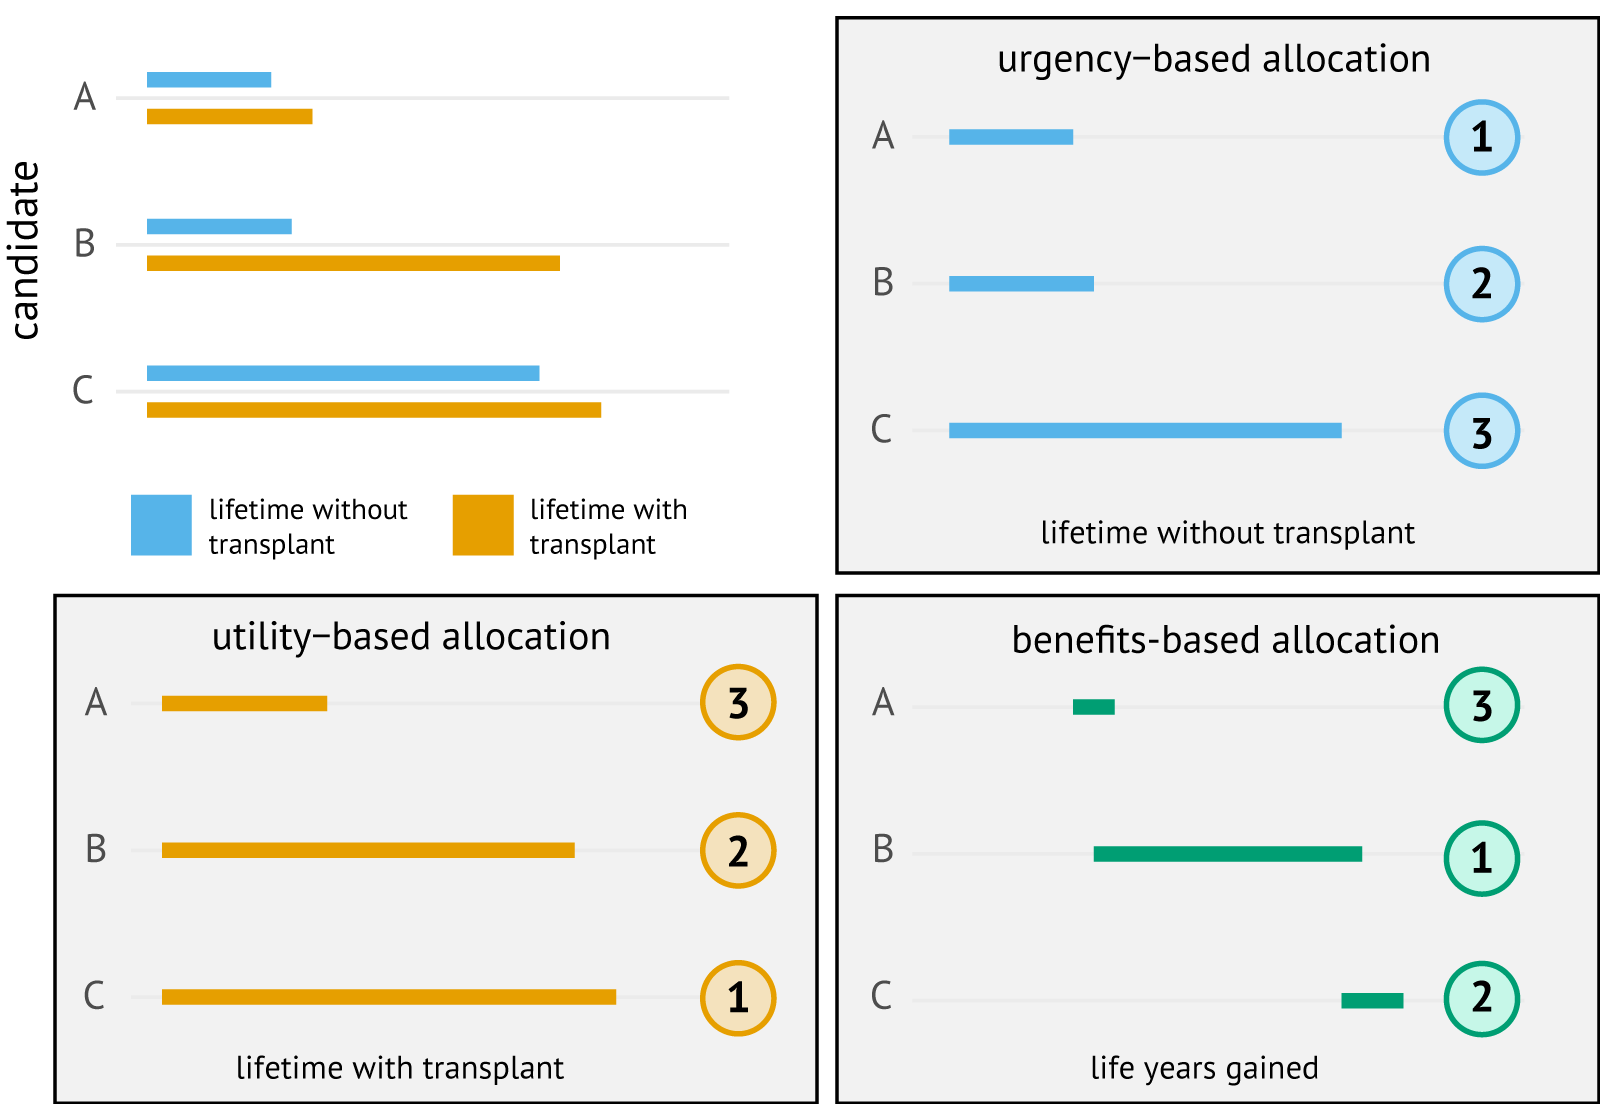
\includegraphics[width=0.95\linewidth]{figures/ch1//fig1-allocation_principles} 

}

\caption{Hypothetical scenario in which a choice has to be made between three
  transplant candidates: candidates A, B, or C. The numbers in circles
  are the ranks for the hypothetical candidates under urgency-based,
  utility-based, and benefits-based allocation.}\label{fig:ch1fig1}
\end{figure}

The third principle, transplant benefit, quantifies which candidate is expected
to benefit most from receiving the organ. Such benefit is typically operationalized
as a contrast between medical utility and medical urgency. For Figure \ref{fig:ch1fig1},
we defined transplant benefit as the number of life years gained by transplantation.
With this definition of benefit, candidate B would be selected for transplantation
by a benefits-based allocation, as they gain the most life years from
transplantation. An
advantage to such an allocation is that it may prevent the transplantation of candidates
who have a short life expectancy after transplantation (candidate A), while
also preventing the transplantation of candidates
who have little need for a transplant (candidate C). Within Eurotransplant, prioritization of candidates for lung transplantation is based on transplant benefit.

Although an allocation that is based on medical utility, medical urgency, or
transplant benefit is conceptually straightforward, applying these principles
for organ allocation is complex. One issue is that the lifetime of transplant
candidates with or without the transplant is not known to Eurotransplant. Allocation
therefore relies on statistical models that quantify a candidate's expected
survival.

\section{Fairness in organ allocation}\label{fairness-in-organ-allocation}

\vspace*{-1em}

Organs are thus allocated in Eurotransplant based on objective medical criteria.
However, prioritizing candidates by solely ranking them on these objective
medical criteria leads to unfair or unjust waiting list outcomes. For instance,
such an allocation would disadvantage candidates with blood group O, who rely on
blood group O donors for access to transplantation, while blood group AB patients
can accept organs from any blood group. With the aim of making allocation more fair,
Eurotransplant has implemented fairness mechanisms in its allocation systems.

One type of fairness mechanisms are the balancing mechanisms that regulate the
international exchange of organs among Eurotransplant's member countries. These
balancing mechanisms were introduced after it was observed that the kidney procurement
and kidney transplant rates were \emph{``totally out of balance''} between Eurotransplant's
member countries, which was deemed unfair to countries with high organ donation rates
\citep{persijnEurotransplantKidneyAllocation2000}. Their continued importance
is underscored by the fact that donor procurement rates still
vary widely between the member countries. For example, Belgium reported
approximately 30 deceased-organ donors per million people per year over the last decade,
while Germany reported only 10 \citep{et_donor_pmp}.
It is deemed just that Belgian patients benefit from the high Belgian donation rate,
and Eurotransplant is even legally required under the Belgian transplantation law
to guarantee a ``reasonable balance'' in the number of organs imported to and exported
from Belgium \citep{BelgischeWet1986}. Such a reasonable balance is ensured by the
balancing mechanisms.

Other fairness mechanisms were implemented to ensure access to transplantation
for specific patient groups \citep{DeMeester1999}. For example, Eurotransplant's liver
allocation system includes ABO blood group rules which give patients access to
roughly the same number of potential donors, regardless of their ABO blood group. This ensures
that no patients are disadvantaged by their own blood group \citep{demeesterWhichABOmatchingRule2002}.
Mechanisms are also in place to facilitate access to transplantation for candidates
for whom a suitable donor is difficult to find. For example, in kidney allocation,
candidates with difficult-to-match leukocyte-antigen typings receive additional
points \citep{demeesterNewEurotransplantKidney1998}.

A separate issue is that some patient groups may be underserved by how medical
urgency, medical utility, or transplant benefit have been defined in
Eurotransplant's allocation systems. For example, several groups of liver
transplant candidates are not at risk of an imminent waiting list death,
which is what is scored by MELD. These candidates may nonetheless require access to
transplantation, for example because of quality of life concerns,
or risk of disease irreversibility.
To help such candidates access transplantation, the liver allocation system awards exception
points to these patient groups. In kidney allocation, prioritization is based on
medical utility because patients with end-stage renal disease can survive for
prolonged periods of time on dialysis. However, some candidates may
lose access to dialysis, and Eurotransplant has implemented rules that facilitate
rapid access to transplantation for such candidates.

There are also patients who may deserve access to transplantation based on
ethical grounds. In Eurotransplant, children have been given special attention.
Another group consists of patients who lose their graft shortly after
an initial transplantation procedure. Special rules
facilitate access to a repeat transplant for these patients.

Considerations of fairness are thus integral to Eurotransplant's current
allocation systems. The importance of fairness was also underscored by the
2007 Joint Declaration that was signed by the Ministers of Health of
Eurotransplant's member countries, which states that maximizing equality of
opportunity for patients is the \emph{``most important factor for allocation''} \citep{ETMan2025}.
Nevertheless, achieving fairness in organ allocation is not a simple task; in describing
Eurotransplant's kidney allocation system, former medical director Guido Persijn
wrote that an allocation system in which transplantation is equally accessible
for all patients is \emph{``very difficult to implement in practice''}, with the
implemented allocation systems merely an \emph{``attempt''} towards this goal \citep{Persijn2006}.

It is thus not surprising that Eurotransplant regularly identifies flaws
in its allocation systems, and revises its systems accordingly. A recent example was the ``blood group O problem'' in kidney
allocation \citep{glander2010}, which arose because Eurotransplant allowed the
transplantation of blood group O kidneys into non-O candidates in case of a perfect
leukocyte-antigen match. Because of this rule, blood group O candidates, who cannot accept non-O
kidneys because of blood group incompatibility, accumulated on the waiting list.
As a result, blood group O candidates faced higher mortality rates than non-O
candidates (13\% vs 8\%) and waited two years longer for a transplant \citep{glander2010}.
This problem was addressed in 2010 by also requiring blood
group identity for perfectly matched donors.
Since then, the gap in waiting times between the blood groups has
shrunk, although blood group O candidates continue to experience longer waiting times
than blood groups A and AB \citep{etStatsLibrary2194P}.
\newpage
The central role of fairness in allocation motivated the first goal of this thesis, which is to
study questions related to equality of opportunity in Eurotransplant's kidney
and liver allocation systems. Specifically,
in Chapter \ref{CHsexdisparity} we study why females are more likely than males
to have an adverse waiting list outcome in liver transplantation, and in Chapter
\ref{CHvpra} we study how immunization affects access to kidney
transplantation. These chapters confirm
that these patient groups are disadvantaged in the current allocation systems.

\section{Challenges in improving organ allocation systems}\label{challenges-in-improving-organ-allocation-systems}

The previous sections discussed that Eurotransplant's allocation systems have
room for improvement. The primary
forums to discuss potential improvements to the allocation systems are
Eurotransplant's organ-specific advisory committees, whose members are
medical specialists who are affiliated with active transplantation programs in Eurotransplant.
These committees can submit recommendations to the
Board of Eurotransplant and national competent authorities on how allocation
may be improved. Before such recommendations are implemented, approval from
these bodies is required.

Changing the allocation systems is a slow process, despite regular meetings
of the advisory committees. One challenge is the complexity of the allocation procedure in
Eurotransplant. When a donor becomes available, Eurotransplant runs computer
algorithms against a central database to generate organ-specific \emph{match lists}.
The transplant centers register their candidates in this database, while
donor procurement organizations register donors in this database. The candidates who are
eligible for the organ offer appear on the match lists, and the order
in which they appear determines the sequence in which Eurotransplant
offers the organs to candidates. Improving the
allocation system may therefore seem as simple as refining the match list order.

However, discussions on the match list order are not straightforward as
match lists behave very differently from regular queuing systems. For example,
being highly ranked on the current match list does not guarantee that a
candidate will attain a similar rank on the next match list.
The top-ranked candidate is also often not transplanted, as the transplant
centers regularly decline organ offers because of concerns about the quality
of the donor, logistical reasons, or temporary non-transplantability of their
patient.

Additional challenges arise from the fact that Eurotransplant's member countries
have different priorities and needs in allocation, in large part because of
the international variation in organ donation rates. For example, Belgium has
more than twice as many organ donors per million people as Germany.
With these varying donation rates, it is often difficult to reach consensus on which
patient groups deserve additional attention. Even when the interests of the
member countries are aligned, it is often not clear how much additional
support a patient group would need to realize equality of opportunity.

Due to these challenges, Eurotransplant's allocation systems evolve only slowly in
response to developments in the field. In fact, the core components of Eurotransplant's
liver and kidney allocation systems have changed little over the past two
decades. For example, kidney allocation in Eurotransplant is still based on
a point system that was introduced in 1996 despite substantial changes in
the waiting list and donor pool. Liver allocation in Eurotransplant has been
based on MELD since 2006, while other regions have switched to different
allocation mechanisms for the liver (e.g., \citep{Allen2024, kimMELD3point0}).

To advance, Eurotransplant requires tools which can give
insight into the adequacy and unintended consequences of proposed policy changes.
This motivated the second goal of this thesis, which is to develop
discrete-event simulation software for this purpose. These simulators replicate the kidney and liver
allocation procedures in Eurotransplant, and were developed in close
collaboration with relevant stakeholders. In Chapters \ref{CHelassimulator}
and \ref{CHetkidneysimulator}, we describe and validate simulators for the
liver and kidney, respectively, and we demonstrate their usefulness through
clinically motivated case studies.

\section{Outline of this thesis}\label{outline-of-this-thesis}

The thesis is divided into two parts. In Part I, we focus on the allocation of the
liver. In Chapter \ref{CHprefaceliver}, we describe the history of
Eurotransplant's liver allocation system and identify potential areas for improvement.
In Chapter \ref{CHdynremeld}, we propose a method that can be used
to revise MELD more efficiently. In Chapter \ref{CHsexdisparity}, we describe
sex disparity in liver waiting list outcomes in Eurotransplant and study the mechanisms
through which this disparity arises. In Chapter \ref{CHelassimulator},
we describe and validate the ELAS simulator, a discrete-event simulator
tailored to Eurotransplant.

In Part II, we turn to allocation of the kidneys. Chapter \ref{CHprefacekidney}
outlines the kidney allocation programs used by Eurotransplant, describes their historical
development, and discusses contemporary challenges in kidney allocation. In Chapter
\ref{CHvpra}, we examine how having a pre-existing sensitization against HLA
antigens affects a candidate's relative transplant rate. In Chapter \ref{CHetkidneysimulator},
we present the ETKidney simulator, a discrete-event simulator for kidney
allocation in Eurotransplant.

We reflect on the findings and contributions of this thesis in Chapter
\ref{CHdiscussion}.

\part{Allocation of the liver}

\chapter{Liver allocation in Eurotransplant}\label{CHprefaceliver}

Liver transplantation is the only curative therapy for patients with acute liver
failure or end-stage liver disease (ESLD), and is the preferred treatment option for
several other liver conditions. The majority of candidates who wait for a liver
transplant have cirrhosis, a chronic liver condition in which inflammation leads
to scarring of the liver. Cirrhosis can be caused by hepatitis B, hepatitis C,
alcohol abuse, metabolic disorders, or a combination thereof \citep{olearyIndicationsLiverTransplantation2008}.
By itself, cirrhosis is not an indication for a liver
transplantation. However, cirrhosis may progress to a stage where the patient
develops clinical symptoms, such as ascites, encephalopathy, or variceal bleeding \citep{olearyIndicationsLiverTransplantation2008}.
With such ``decompensating'' symptoms, liver transplantation can be indicated.
Eventually, decompensated cirrhosis may progress into multiple organ failure
-- a syndrome now recognized as acute-on-chronic liver failure (ACLF),
which is associated with a high short-term mortality risk \citep{Arroyo2020}.

Cirrhosis is also a risk factor for developing hepatocellular carcinoma (HCC),
the most common form of liver cancer. While most patients with HCC have cirrhosis,
they typically have a well-preserved liver function \citep{olearyIndicationsLiverTransplantation2008}.
Despite not having progressed to ESLD, these candidates may require a
liver transplantation to prevent tumor progression and to reduce the risk of
tumor recurrence after transplantation. For patients with HCC who meet the internationally
accepted Milan criteria, liver transplantation is internationally recognized as
the most effective surgical therapy \citep{Galle2018}.

Besides cirrhosis, there are many other conditions that can be an indication
for liver transplantation. One group of patients who urgently require access
to transplantation consists of patients with acute liver failure (ALF).
Acute liver failure is characterized
by an unexpected and abrupt loss of liver function, which can be triggered by
among others acute viral hepatitis, mushroom poisoning, or paracetamol intoxication. Without
transplantation, patients with ALF are expected to die within days \citep{stravitzAcuteLiverFailure2019}.
Examples of chronic, non-cirrhotic indications are polycystic liver disease and cholestatic
liver disease. Polycystic liver disease is a genetic
disorder that causes cysts to grow in the liver and predominantly affects females.
Although polycystic liver disease is not life-threatening, the condition can
cause debilitating symptoms that may justify liver transplantation.
One type of cholestatic liver disease is primary sclerosing cholangitis (PSC),
which has a higher incidence in males. PSC is characterized by inflammation of the bile ducts
which leads to scarring. If PSC is recurrent, liver transplantation may be indicated
because it is a pre-stage for cholangiocarcinoma and associated with a
reduced quality of life \citep{olearyIndicationsLiverTransplantation2008}.

This far-from-exhaustive overview of indications for liver transplantation
shows that the liver waiting list consists of heterogeneous groups of patients, who require access to liver transplantation for different reasons. Designing a
liver allocation system that adequately serves these heterogeneous patient
groups is a difficult task. In this chapter, we describe how Eurotransplant
has tried to balance the interests of these patient groups.

\section{Liver allocation prior to MELD}\label{liver-allocation-prior-to-meld}

In the 1990s, Eurotransplant had limited involvement in the allocation of livers.
In fact, the exchange of livers was mandatory only
for candidates who had a High Urgency
(HU) status \citep{HaaseKromwijk1999}. Candidates with acute liver failure or other
\emph{de novo} life-threatening conditions were eligible for this status. If
no such candidates were available for transplantation, the transplantation
center responsible for procurement of the liver could freely select a candidate
from their own waiting list for transplantation (subject to blood group rules) \citep{demeesterWhichABOmatchingRule2002}. If the procurement center did not have
suitable candidates available, Eurotransplant used a rotation system to
offer the liver to other centers. Contacted centers could again freely select
a candidate from their waiting list for transplantation \citep{Jost1997, Chapman1997}.
How candidates were prioritized was thus mostly left to the discretion of
the transplant centers.

In July 2000, Eurotransplant introduced a patient-oriented allocation system
for the liver \citep{Strassburg2004}, as was required under the Dutch and
German transplantation laws that were introduced in the 1990s \citep{HaaseKromwijk1999}. In this system, candidates for liver
transplantation were categorized into four medical urgency groups: high urgency
(T1), chronic disease with acute decompensation (T2), chronic disease with
complications (T3), or chronic disease without complications (T4). Candidates
with a T1 status received international priority, while elective candidates (T2-T4) were prioritized
using a point system that awarded points for the candidate's medical urgency (T2-T4), their waiting time, and their location relative to the donor \citep{minutesELIACMeeting2002}.
Candidates were categorized into a T2, T3, or T4 status based on their Child-Pugh
score, which can be used to assess the prognosis of candidates with cirrhosis \citep{Strassburg2004, Jung2008}.

The most important disadvantage of this patient-oriented system was that waiting
time had a dominant role \citep{Strassburg2004, Jung2008}, which incentivized the
transplant centers to refer their candidates early for transplantation. In Eurotransplant,
this contributed to a tenfold increase in the number of candidates who
waited for liver transplantation between 1991 and 2006 \citep{Jung2008}. As a result,
waiting times in Germany exceeded 200 days even for candidates with a T2 status,
who by definition have acute decompensation \citep{Strassburg2004}. With
these waiting times, it was observed that the candidates with the shortest
waiting times faced an increased risk of dying \citep{minutesELIACMeeting2002}. This
indicated that the allocation system failed to adequately rank candidates on
medical urgency.

Classifying medical urgency based on the Child-Pugh score was also contentious
because these scores are partially based on a subjective assessment of the candidate's
encephalopathy grade and ascites grade \citep{Jung2008, wiesnerModelEndstageLiver2003}.
Concerns were voiced in the Eurotransplant Liver and Intestine Committee (ELIAC)
that centers abused these subjective criteria, and \emph{``tried to push their candidates into
a T2 status''} \citep{minutesELIACMeeting2006}. Moreover, ascites and encephalopathy
are also specifically linked to cirrhosis, such that candidates with
other liver conditions were typically assigned a T4 status \citep{Strassburg2004}.
Consensus in ELIAC was that this was unfair to candidates with hepatocellular
carcinoma or metabolic disorders \citep{minutesELIACMeeting2001}.

\section{MELD-based liver allocation in the United States}\label{meld-based-liver-allocation-in-the-united-states}

In the United States, a similar liver allocation system had been in use since 1998.
This system also prioritized candidates using four medical urgency categories
that were based on the Child-Pugh score. Freeman et al.~(2004) reported that
under this system there was \emph{``virtually no relation between waiting time and
mortality for each medical urgency status''}. This finding -- reported on behalf
of UNOS, the organ allocation organization of the United States -- motivated a
search for an alternative disease severity score that could be used to prioritize
candidates for liver transplantation. This disease severity score would become
the Model for End-stage Liver Disease (MELD) score, which was implemented in 2002.

Notably, this MELD score was not originally developed to predict survival on the
liver transplantation waiting list. Instead, MELD was developed by Malinchoc et al.~(2000)
to predict 90-day survival after an elective transjugular intrahepatic porto-systemic
shunt (TIPS) procedure \citep{malinchocModelPredictPoor2000}. These procedures are
indicated in cirrhotic patients with acute decompensation to prevent variceal
rebleeding, or to treat refractory ascites. Malinchoc et al.~demonstrated that
this model outperformed the Child-Pugh score in predicting 90-day survival after TIPS.
\newpage
Whether this scoring system could also be used to rank candidates for liver
transplantation was first studied by Kamath et al.,
who showed that MELD could also predict the 90-day mortality of three
other cirrhotic patient groups: hospitalized cirrhotic
patients who did not undergo a TIPS procedure, ambulatory patients with cirrhosis,
and patients with biliary cirrhosis \citep{kamathModelPredictSurvival2001}.
Furthermore, Kamath et al.~showed that
including clinical symptoms or disease etiology only minimally improved the model's
predictive performance, which meant that survival could be
adequately predicted based on blood-based biomarkers alone. Candidates for
liver transplantation could thereby be prioritized solely based on objective
medical criteria, which was considered advantageous. Subsequent external validations have
demonstrated that MELD is indeed superior to the Child-Pugh score for predicting
90-day survival on the liver waiting list
\citep{wiesnerModelEndstageLiver2003}.

Based on these findings, a policy to prioritize patients using MELD was approved
in the United States in November 2001. Under this system, which was implemented
in February 2002, MELD scores are calculated based on measurements of
serum bilirubin (mg/dl),
serum creatinine (mg/dl) and the International Normalized Ratio (INR)
of prothrombin time, using the following formula:

\[6.43\  + 3.78\ln\left( \text{bilirubin} \right) + 9.57\ln\left( \text{creatinine} \right) + 11.20\ln\left(\text{INR}\right).\]

In calculating MELD scores, the laboratory measurements for biomarkers are set to
a minimum of 1 to prevent negative scores. UNOS also proposed to cap
serum creatinine at 4.0 mg/dl, to limit MELD scores to a maximum of 40, and to
rank candidates by their rounded MELD scores. Because of these choices, MELD
scores range from 6 to 40.

It was anticipated that a purely MELD-based allocation would underserve
candidates with metabolic disease, cholestatic liver disease, or hepatocellular carcinoma
\citep{kamathModelPredictSurvival2001, wiesnerModelEndstageLiver2003}.
To help such candidates access transplantation, policymakers in the United States
also introduced an elaborate exception point system that awards exception points
for various non-cirrhotic indications.

\section{MELD-based liver allocation in Eurotransplant}\label{meld-based-liver-allocation-in-eurotransplant}

In 2003, the ELIAC recommended assessing whether MELD could replace the Child-Pugh
score for liver allocation in Eurotransplant \citep{Jung2008}. Following this
recommendation, delegates from Eurotransplant visited UNOS in 2003 and 2004 to
study how a MELD-based allocation system could be adapted for Eurotransplant.
These visits ultimately led to the introduction of MELD-based liver allocation in
Eurotransplant in December 2006.
\newpage
Because of these visits, the core of Eurotransplant's MELD-based liver allocation
system closely mirrors UNOS' implementation. For example, both systems give
priority to candidates with acute liver failure and prioritize ``elective''
(i.e., non-HU) candidates using MELD scores. In both systems, prioritization is
based on the \emph{``match-MELD''} score, which is the maximum of the \emph{``lab-MELD}'' score
(calculated from biomarkers) and exception points. Eurotransplant also
uses the exact same formulas as UNOS to calculate the lab-MELD and exception scores.

Within MELD-based liver allocation in Eurotransplant, international sharing is mandatory
only for candidates with a High Urgency (HU) status and those awaiting a combined
transplantation. Otherwise, candidates located in the same country as the donor
have priority in Eurotransplant. A distinctive feature of Eurotransplant's
liver allocation system is
that an obligation system was introduced, which ensures that livers exported
with international priority are paid back by the importing country \citep{jochmansAdultLiverAllocation2017}.
Another difference lies in the prioritization of pediatric candidates: within
Eurotransplant, children are prioritized with exception points, while UNOS
uses PELD, a disease severity score developed specifically for children
\citep{freemanImprovingLiverAllocation2004}.

MELD-based liver allocation in Eurotransplant has to abide by the national regulations
of its member countries, which introduces considerable complexity into the
allocation system. For example, only in Germany and the Netherlands is the ranking
of candidates completely based on the match-MELD. In Austria, Croatia, Hungary
and Slovenia, procurement centers are still allowed to select a candidate from
their own waiting list, as was the case under the center-based allocation system
of the 1990s. In Belgium, a mixture of center- and patient-based allocation
is used, with centers free to select a candidate for Donation after Cardiac Death
(DCD) donors, but not for Donation after Brain Death (DBD) donors \citep{jochmansAdultLiverAllocation2017}.
National competent authorities have varying opinions regarding which indications deserve
to be prioritized with exception points. To accommodate these different views,
Eurotransplant's member countries have completely separate exception point systems, with exception
points valid only for national allocation.

\section{Areas for improvement in MELD-based allocation systems}\label{areas-for-improvement-in-meld-based-allocation-systems}

Since Eurotransplant switched allocation by MELD in December 2006,
several potential areas for improvement for MELD-based liver allocation have been
identified. One known limitation of MELD is that
it underestimates the waiting list mortality risks for certain
cirrhotic patient groups. These include candidates with low serum sodium
levels (hyponatremia) \citep{kimHyponatremiaMortalityPatients2008a}. This has motivated
UNOS to switch in 2016 to liver allocation based on the MELD-Na score, which adds
serum sodium to the MELD formula. A second patient group consists of female transplantation
candidates, who are more likely to have an adverse waiting list outcome than males
in the United States \citep{moylanDisparitiesLiverTransplantation2008}. To address
this disparity, UNOS liver allocation has become based on MELD 3.0 in 2023, which
adds serum albumin to the formula and adds 1.33 to the MELD score of female transplant candidates \citep{kimMELD3point0}. In Chapter \ref{CHsexdisparity}, we examine whether
females are also more likely to face an adverse waiting list outcome in
Eurotransplant, and assess why that would be the case.

A second area of improvement concerns the formula that is used to calculate MELD scores.
The coefficients in this formula were based on a Cox proportional hazards model
that was developed for the prediction of survival after a TIPS procedure, not survival
on the liver waiting list. A rich literature exists which seeks to re-estimate
these coefficients on candidates for liver transplantation \citep{merionLongitudinalAssessmentMortality2003, sharmaReweightingModelEndStage2008, leiseRevisedModelEndstage2011}.
A related area of criticism concerns the choices that UNOS has made in introducing MELD,
such as capping creatinine at 4.0 mg/dl and
calculating MELD with minimum values of 1 for all biomarkers. Studies have
argued that these choices lacked empirical support and have revised these
upper and lower limits \citep{leiseRevisedModelEndstage2011}. For Eurotransplant specifically,
Goudsmit et al.~proposed ReMELD and ReMELD-Na, which were scores obtained by
revising MELD and MELD-Na with retrospective data from Eurotransplant \citep{goudsmitRefittingModelEndstage2020}. In a case study in Chapter \ref{CHelassimulator}, we assess how implementation
of the ReMELD-Na score would affect waiting list outcomes in Eurotransplant.

The studies that revise MELD based on liver transplant candidate data typically
associate a candidate's 90-day waiting list survival with their MELD biomarkers
reported at listing. This approach inefficiently uses the data that is available
at Eurotransplant, because most candidates have multiple sets of MELD biomarkers
available as centers are required to regularly recertify the MELD scores of their candidates.
In Chapter \ref{CHdynremeld}, we assess how this information
can be used to revise MELD more efficiently.

A third potential area of improvement is that the prioritization of candidates based on a
sickest-first principle may result in transplanting candidates who
have a short life expectancy after transplantation. In Eurotransplant, mixed results exist as to
whether allocation based on MELD leads to worse post-transplant outcomes \citep{Nagler2005, Weismller2009}.
At least in theory, an allocation based on transplant benefit could help prevent such futile
transplantations. Such a benefits-based allocation system was first proposed in
the United States by Schaubel et al. \citep{Schaubel2009}, but it was never implemented.
In the United Kingdom, allocation of livers has become
based on the \emph{Transplant Benefit Score} (TBS) since 2018 \citep{Allen2024}. TBS has
been contentious because it underserved candidates with HCC \citep{Attia2023} and
it is thought to have reduced access to transplantation for young liver
transplant candidates \citep{Attia2024}.

A fourth area of improvement is the exception point system that is used to prioritize
non-cirrhotic candidates for transplantation. In the United States,
studies have reported that candidates eligible for exception points were overprioritized
\citep{Massie2011, Goldberg2014}, which has led to a substantial deprioritization of
candidates with exception points in OPTN, which is the national system that manages organ
allocation in the United States. For example, UNOS first lowered the number
of points awarded to candidates with HCC in 2003, which was followed by removal
of exception points for those with stage I HCC. In 2005, the priority for candidates with stage II HCC was again
lowered, which was followed by a ``Delay and Cap'' policy for HCC in 2015
\citep{pillaiLiverAllocationPolicies2019}. With this policy, candidates
with HCC would not be eligible for exception points until they had waited six months
for a liver transplant (the ``delay''), and would receive a maximum exception score of 34 points
on the MELD scale (the ``cap''). In 2019, UNOS completely removed the 90-day upgrades for all exception points,
a decision motivated by findings that these 90-day upgrades were linked to an increase in the
median MELD score at transplantation of 22 in 2005 to 27 in 2012 \citep{northupExcessMortalityLiver2015}. To counter such ``MELD inflation'', candidates
with exceptions are now awarded a fixed number of points in the United States,
which is specified relative to the median MELD at transplantation (MMAT) \citep{Bonner2018}. For HCC, this number is
set to the MMAT minus three points.

In Eurotransplant, in contrast, changes to the exception point system have been adopted only sporadically. For example, only in the Netherlands was a six-month waiting period
adopted for HCC, analogous to UNOS's 2015 ``Delay and Cap'' policy.
This lack of policy reform is surprising because several articles
have suggested that candidates with exception points are also overprioritized in Eurotransplant
\citep{Goet2017, Metselaar2017}. Notable in this regard is a study by Umgelter et al. \citep{umgelterDisparitiesEurotransplantLiver2017a},
who concluded on behalf of ELIAC that patients with exception points appear to be
advantaged compared to candidates without exception points. In Chapter
\ref{CHelassimulator}, we examine how
changes to the exception point system would affect waiting list outcomes in
Belgium, the country in which most exceptions are awarded within Eurotransplant.

As this chapter sets out, the literature is rich with ideas on how MELD-based
liver allocation can be improved. A major barrier to implementing these ideas is
that Eurotransplant has lacked the tools to quantitatively assess how a change
in allocation rules would impact the
liver waiting list outcomes. To fill this gap,
we developed a discrete-event simulator that mimics the liver allocation system in Eurotransplant.
We describe this simulator in detail in Chapter \ref{CHelassimulator}.

\chapter{Revising MELD from calendar-time cross-sections with correction for selection bias}\label{CHdynremeld}

\chaptermark{DynReMELD}

\vfill

\begin{center}\rule{0.5\linewidth}{0.5pt}\end{center}

\noindent
An article based on this chapter has appeared in \emph{BMC Medical Research Methodology}, de Ferrante, H.C., De Rosner-van Rosmalen M., Smeulders, B.M.L., Vogelaar, S., Spieksma, F.C.R., 2024, \href{https://doi.org/10.1186/s12874-024-02176-8}{10.1186/s12874-024-02176-8},
\citep{deFerranteDynremeld}

\newpage
\normalsize

\subsubsection*{Abstract}

Eurotransplant allocates livers using the MELD score as originally proposed
by UNOS. Several studies have revised this UNOS-MELD score using retrospective
data on liver transplant candidates. The standard approach taken in such studies is to model 90-day
waiting list mortality from the time of listing, based on biomarkers reported at
listing, while censoring candidates at delisting or transplantation. This approach
ignores a candidate's biomarkers that were reported after registration, and ignores informative
censoring by transplantation and delisting.

We study how MELD revision is affected by using calendar-time
cross-sections and by correcting for informative censoring with inverse
probability censoring weighting (IPCW). To this end, we revised UNOS-MELD
on patients with cirrhosis who were on the Eurotransplant waiting list
between 2007 and 2019 (n=13,274) with Cox models with as endpoints
90-day survival (a) from registration and (b) from weekly drawn
calendar-time cross-sections. We refer to the score revised from
cross-section with IPCW as \emph{DynReMELD}. We compare DynReMELD to
UNOS-MELD and ReMELD, a prior revision of UNOS-MELD for Eurotransplant,
in a geographical validation.

Our results show that revising MELD from calendar-time cross-sections leads to significantly
different MELD coefficients. IPCW increases estimates of absolute 90-day
waiting list mortality risks by approximately 10 percentage points.
DynReMELD shows improved discrimination compared to UNOS-MELD (delta c-index:
0.0040, p\textless0.001) and ReMELD (delta c-index: 0.0015, p\textless0.01), with
differences comparable in magnitude to the addition of an extra
biomarker to MELD (delta c-index: ±0.0030).

Correction for selection bias by transplantation or delisting with inverse
probability censoring weighting does not
improve the discrimination of revised MELD scores, but does substantially
increase estimates of absolute 90-day mortality risks. Revision from
cross-section uses waiting list data more efficiently, and improves
discrimination compared to revision of MELD exclusively based on
the information available at listing.

\newpage

\section{Introduction}\label{introduction}

Eurotransplant calculates MELD scores with a formula originally introduced by
UNOS in 2002. We refer to this score as UNOS-MELD. Various limitations of UNOS-MELD
have been described, including that

\begin{enumerate}
\def\labelenumi{\arabic{enumi}.}
\item
  it was not developed to predict mortality on the liver waiting list \citep{malinchocModelPredictPoor2000},
\item
  it overemphasizes renal dysfunction
  \citep{sharmaReweightingModelEndStage2008},
\item
  it uses biomarker caps that are not evidence-based
  \citep{leiseRevisedModelEndstage2011},
\item
  it is poorly calibrated for specific subgroups, such as
  patients with hyponatremia \citep{kimHyponatremiaMortalityPatients2008a}.
\end{enumerate}

These limitations have motivated several studies to revise MELD, either
by re-estimating the equation's coefficients using registry data on
liver transplant candidates (e.g., \citep{sharmaReweightingModelEndStage2008, leiseRevisedModelEndstage2011}), or by expanding the scoring system
with new biomarkers (e.g., MELD-Na
\citep{kimHyponatremiaMortalityPatients2008a} or MELD 3.0
\citep{kimMELD3point0}). In 2020, the equation's coefficients and caps of MELD
were revised by Goudsmit et al.~using retrospective data from Eurotransplant.
The resulting score is referred to as the ``ReMELD'' score \citep{goudsmitRefittingModelEndstage2020}.

MELD revision typically proceeds by modeling waiting list mortality up to
90 days after waiting list registration based on biomarkers reported at
registration (e.g., \citep{leiseRevisedModelEndstage2011, kimHyponatremiaMortalityPatients2008a, kimMELD3point0, goudsmitRefittingModelEndstage2020}). This \emph{``from registration''} approach
poorly aligns with the clinical use of MELD: in allocation, candidates are prioritized
on their last reported MELD score, and not on the MELD score that was reported at listing. Moreover, revising MELD \emph{``from registration''} ignores
waiting list deaths that occur more than 90 days after listing, which are
two-thirds of all liver waiting list deaths within Eurotransplant.

Previously, such waste of statistical information was avoided by
adjusting for MELD biomarkers as time-varying covariates
(\citep{sharmaReweightingModelEndStage2008, merionLongitudinalAssessmentMortality2003}).
However, MELD biomarkers also increase as part of the death process
\citep{bambhaPredictingSurvivalPatients2004}, such that use of
MELD biomarkers as time-varying covariates leads to issues of reverse
causality. This reverse causality problem is exacerbated by the fact that MELD scores can be updated voluntarily at any time and by the fact that sicker patients are required
to update their MELD scores more frequently.

To prevent these issues, we propose revising MELD \emph{``from cross-section''}
using methodology developed by Gong and Schaubel
\citep{gongPartlyConditionalEstimation2013}. With this approach MELD is
revised by modeling the remaining time-until-death from pre-specified
calendar-time cross-sections rather than from registration. Biomarkers
measured after listing and deaths recorded more than 90
days after listing thereby inform MELD revision. To prevent issues of reverse
causality, adjustment at each cross-section is for historical biomarker
information only. The evolution of biomarkers after the cross-section
date affects survival, transplantation and delisting rates, which makes
transplantation and delisting informative censoring mechanisms. Prior revisions
of MELD censor patients at transplantation or delisting, which introduces
bias. We study how MELD revision is
affected by correcting for dependent censoring with inverse
probability censoring weighting, which was first proposed by Gong and Schaubel \citep{gongPartlyConditionalEstimation2013}.

\section{Materials and methods}\label{materials-and-methods}

\subsection{Study population and data}\label{study-population-and-data}

Adult patients with any active waiting list status on the Eurotransplant
waiting list between December 16, 2006, and December 31, 2019, were extracted from
the Eurotransplant database. Only patients with cirrhosis were included
in the study, which is the patient group on which UNOS-MELD was originally
validated. Patients with other diagnoses, those prioritized through exception
points, and those awaiting a repeat transplantation or combined transplantation
were excluded (except combined liver-kidney transplantation
candidates). Patients with impossible values for MELD biomarkers (e.g., all
zeroes for bilirubin, creatinine, and the INR) were excluded.

To activate a candidate on the liver waiting list, centers have to report MELD
biomarkers to Eurotransplant. Reported MELD scores are valid for a maximum of one
year, and expire in a shorter time window for sicker patients (within seven days for MELD scores greater than 25
\citep{ETLiverMan2025}). Failure to update the MELD score results in the
lowest possible MELD score of 6 being used for allocation. Consequently,
MELD updates are available for most transplant candidates in the Eurotransplant
database. Centers can set
candidates to non-transplantable (NT) if they are temporarily not available
for transplantation, which ensures that the transplant center is not
contacted with offers for these patients.

\subsection{MELD scores, UNOS-MELD and ReMELD}\label{meld-scores-unos-meld-and-remeld}

We define a MELD scoring system as a system that calculates a score based
on serum bilirubin, serum creatinine and the INR, using the following formula:

\[\text{intercept}\  + \text{coef}_{\text{bili}}\ln\left( \text{bili} \right) + \ \text{coef}_{\text{crea}}\ln\left( \text{crea} \right) +
\text{coef}_{\text{INR}}\ln\left( \text{INR} \right),\]

with serum bilirubin and serum creatinine measured in mg/dl. A specific MELD
score proposes values for the intercept and coefficients, and bounds for the
values of MELD biomarkers. A MELD score also has to propose how to calculate
MELD scores for candidates who received dialysis twice in the week before
measurement of MELD biomarkers (henceforth ``patients on biweekly dialysis''),
since dialysis reduces measured creatinine levels. Eurotransplant currently uses UNOS-MELD for allocation, i.e.

\[6.43\  + 3.78\ln\left( \text{bilirubin} \right) + 9.57\ln\left( \text{creatinine} \right) + 11.20\ln\left( \text{INR} \right),\]

in which creatinine is capped at 4.0 mg/dl, a lower limit of 1.0 is imposed on
all biomarkers, and creatinine is set to 4.0 mg/dl for patients on biweekly
dialysis.

Various revisions of MELD have been proposed (e.g., see
\citep{leiseRevisedModelEndstage2011, goudsmitRefittingModelEndstage2020, bambhaPredictingSurvivalPatients2004}).
One alternative -- that was
developed specifically for Eurotransplant -- is ReMELD
\citep{goudsmitRefittingModelEndstage2020}, which calculates the score as

\[8.422\  + 7.728\ln\left( \text{bili} \right) + \ 3.446\ \ln\left( \text{crea} \right) + 10.597\ln\left( \text{INR} \right).\]

In calculating ReMELD scores, bilirubin is bounded between 0.3 and 27 mg/dl, the INR is
bounded between 0.1 and 2.6, and creatinine is bounded between 0.7 and 2.5 mg/dl. Creatinine is
also set to the upper cap of 2.5 mg/dl for patients on biweekly dialysis.

\subsection{\texorpdfstring{Revision \emph{``from registration'' vs.~``revision from cross-section''}}{Revision ``from registration'' vs.~``revision from cross-section''}}\label{revision-from-registration-vs.-revision-from-cross-section}

In revising MELD, authors typically re-estimate MELD coefficients \emph{``from
registration''}. By this, we mean that authors use Cox proportional hazards models
to model 90-day waiting list mortality after registration with adjustment
for MELD biomarkers that were reported at listing. Coefficients for the MELD scoring system are then commonly derived by rescaling the estimated regression coefficients (\(\widehat{\beta}\)) to the UNOS-MELD scale. This rescaling is typically achieved by matching quantiles of the linear predictor to corresponding quantiles of UNOS-MELD scores (e.g., \citep{leiseRevisedModelEndstage2011, goudsmitRefittingModelEndstage2020}).
This \emph{``from registration''} approach ignores any MELD measurements recorded after registration, as
well as patient deaths recorded more than 90 days after registration. We
propose to avoid such waste of statistical information by revising
MELD with a \emph{``from cross-section''} approach. The key differences between these
approaches are illustrated in Figure \ref{fig:ch3fig1}.

The \emph{``from cross-section''} approach uses methodology developed by Gong and Schaubel
\citep{gongPartlyConditionalEstimation2013}, and models the remaining
time-until-death from pre-specified calendar-time cross-sections (see
right panel, Figure \ref{fig:ch3fig1}). This approach uses cross-section calendar
times as the time origin, and the time elapsed since the cross-section date as
the timescale. The coefficients are estimated with a Cox proportional hazards model
that is stratified by the cross-section. At each cross-section only
patients with an active registration (i.e., without non-transplantable
status) are included in the analysis, and Cox models adjust only for
biomarker information reported \emph{before} the cross-section. We point out
that patients waiting at multiple calendar-time cross-sections
contribute multiple observations to the Cox model fit (right panel,
Figure \ref{fig:ch3fig1}). Thereby, revision of MELD is also affected by (i)
waiting list deaths that occur more than 90 days after listing, and (ii)
biomarker measurements taken after listing.

\vfill

\begin{figure}[h]

{\centering 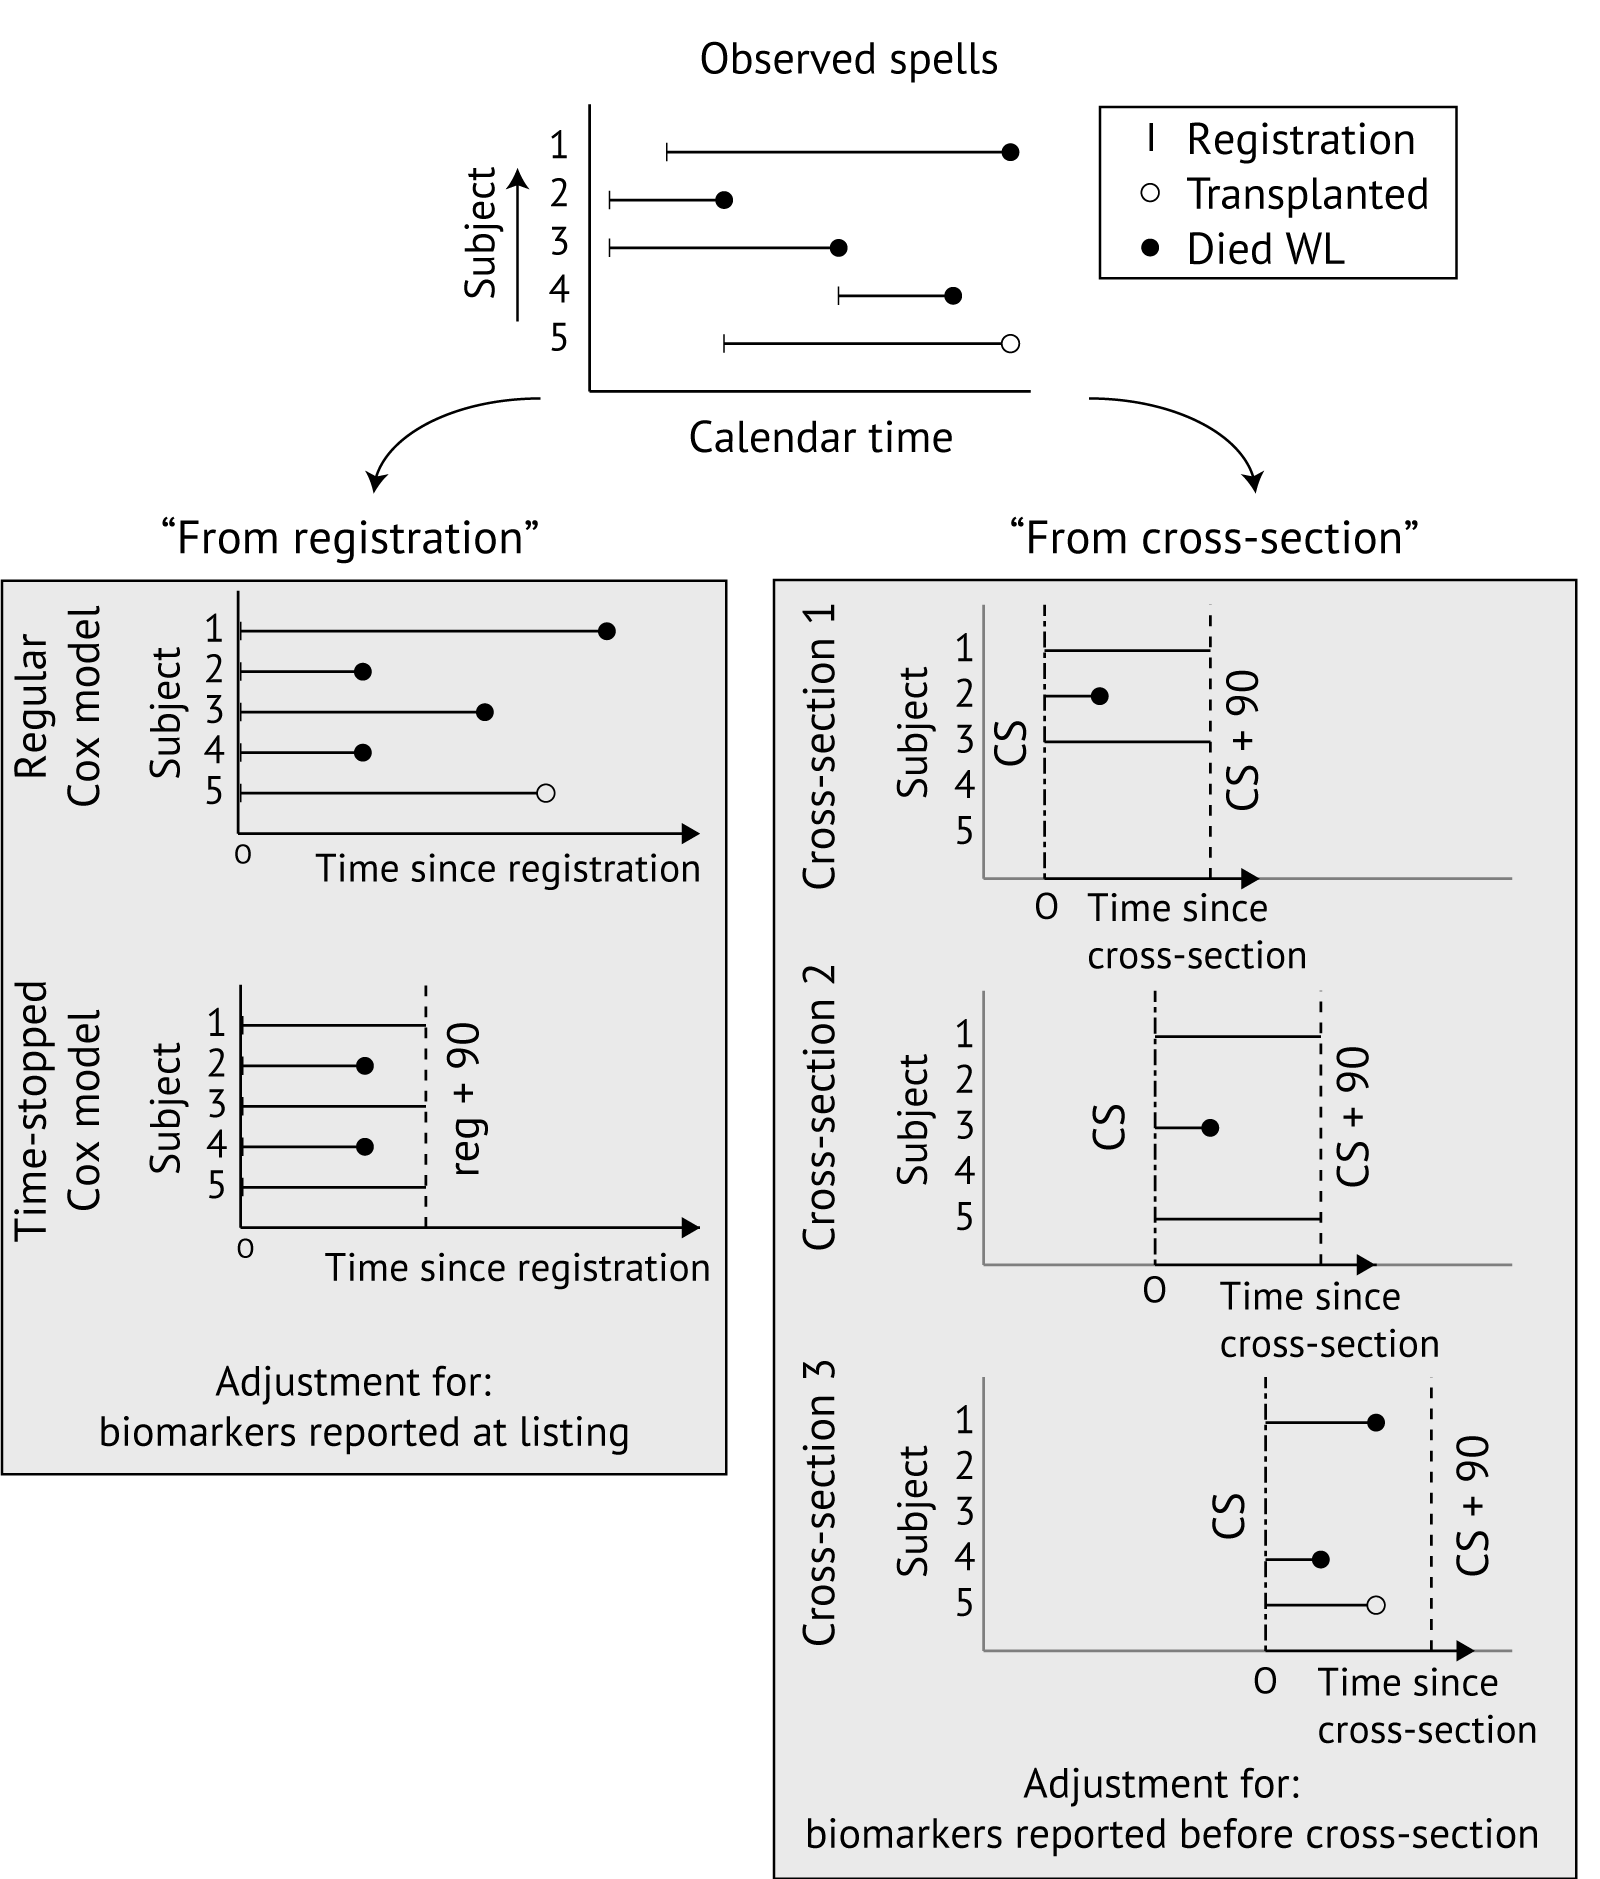
\includegraphics[width=0.87\linewidth]{figures/ch3//figure1} 

}

\caption{Illustration of from “registration” and “from cross-section” approaches to modeling waiting list mortality. For revision of MELD, typically 90-day time-stopped Cox models are used. The “from registration” approach (left) uses time since registration as the timescale and adjusts for biomarkers reported at registration. The “from cross-section” approach (right) models time-until-death from cross-section dates, pre-specified in calendar time, and adjusts for MELD biomarkers reported before the cross-section date. WL, waiting list.}\label{fig:ch3fig1}
\end{figure}

\FloatBarrier
\newpage

In this chapter, we compare revision of MELD \emph{``from
registration''} to revision \emph{``from cross-section''}. In revising MELD
\emph{``from registration''}, we stratify models by country of listing. For the
\emph{``from cross-section''} approach, we use weekly cross-sections from
December 22, 2006 to December 31, 2019 and stratify Cox models by the
candidate's country of listing and
by cross-section. The candidate survival status 90 days after the cross-section date is
used as an endpoint, and adjustment at each cross-section is for the
last reported MELD biomarker values before the cross-section date.

\subsection{Outcome definition}\label{outcome-definition}

Time-until-death is modeled with 90-day time-stopped Cox PH
models. Delisted patients who die within 90 days of deregistration are
treated as if they had died on waiting list exit (as in
\citep{goudsmitRefittingModelEndstage2020}). Patients who were
transplanted or delisted within 90 days are censored.
Inverse probability censoring weighting (IPCW) is used to correct for
selection bias due to transplantation and delisting.

\subsection{Inverse probability censoring weighting to correct for dependent censoring}\label{inverse-probability-censoring-weighting-to-correct-for-dependent-censoring}

Consistent estimation of parameters \(\beta\) with a standard Cox PH model
requires that the censoring process is independent of survival,
conditional on covariates. This independent censoring
assumption is violated for both the \emph{``from registration''} and \emph{``from
cross-section''} approaches, because only MELD biomarkers
reported at listing (or before the cross-section date) are included as covariates, while MELD biomarkers
reported after listing (or cross-section) affect patient survival and transplantation/delisting rates.
Gong and Schaubel proposed a procedure
that can correct for the bias introduced by dependent censoring due to transplantation.
This procedure weighs candidates by their inverse probability of having been transplanted
between the cross-section and exit date (IPCW-T weights, T for transplantation).
Such probabilities can be estimated using an extended Cox proportional hazards model, which
uses the candidate's transplantation status as the outcome.

We expand in this chapter on Gong and Schaubel's approach by also
constructing inverse probability censoring weights for delisting
(IPCW delisting (IPCW-D) weights). Under the assumption that delisting
and transplantation are conditionally independent, a joint inverse
probability censoring weight can then be obtained by multiplying
IPCW-T and IPCW-D weights (see also \citep{schnellingerMitigatingSelectionBias2021}). Details on how weights
were constructed are included in Appendix \ref{APPipcw}. In this chapter, we assess
how IPCW affects revised MELD coefficients both \emph{``from registration''}
and \emph{``from cross-section''}.

\vfill

\subsection{Adjustment variables, caps, and functional forms}\label{adjustment-variables-caps-and-functional-forms}

Cox PH models adjust for variables present in MELD, i.e., serum bilirubin,
serum creatinine, and the INR. Spline terms are used to assess
whether the relation between log-transformed biomarkers and the
mortality rate is approximately linear. Final models use
logarithmic transformations for the biomarkers, with lower and upper
limits for biomarkers optimized over regions where violation of
log-linearity was visually apparent (as in
Leise et al. \citep{leiseRevisedModelEndstage2011} and Goudsmit et al.~
\citep{goudsmitRefittingModelEndstage2020}).

On the Eurotransplant liver waiting list, more than 10\% of patients receive biweekly dialysis, and
measured creatinine is not used to calculate lab-MELD scores for these patients.
To also ignore measured creatinine in revising MELD for these patients, we set
creatinine to 1.0 mg/dl for patients on dialysis (leading to \(\ln(1.0) = 0\) MELD points).
Instead, we use whether the patient receives biweekly dialysis as an adjustment variable.

\subsection{Development and validation cohorts}\label{development-and-validation-cohorts}

To enable revision and geographical validation for all Eurotransplant countries,
we aimed to use a 70\%/30\% center-based split per country. Such a
split was feasible for Germany (70\%/30\%), Belgium (70.1\%/29.9\%)
Austria (62.6\%/37.4\%), and the Netherlands (74.3\%/25.7\%), but not for
Hungary (1 center), Slovenia (1 center), and Croatia (1 large center, 2
very small centers). Therefore, Hungarian, Slovenian and Croatian
patients (11\% of the total cohort) were randomly split into 70\%/30\%
development/validation cohorts.

All models -- including those used to estimate inverse probability
weights -- were fitted on the development cohort only. The validation
cohort was used to compare the newly developed score -- which we name \emph{DynReMELD} -- to
ReMELD and UNOS-MELD.

\subsection{Comparison to UNOS-MELD and ReMELD}\label{comparison-to-unos-meld-and-remeld}

We revised MELD \emph{``from registration''} and \emph{``from cross-section''} both
with and without IPCW. Without IPCW, MELD was also revised with ReMELD's
linear predictor used as an offset. This enables assessment of whether
revision of MELD on all cirrhotic patients yields a significantly
different equation from ReMELD. We define \emph{DynReMELD} as the equation
obtained by quantile matching the linear predictor revised \emph{``from
cross-section''} with IPCW to quantiles of UNOS-MELD.
\newpage
We compare the discrimination of MELD, ReMELD and DynReMELD using the c-index
in the validation cohort. This c-index quantifies the degree to which patients with a
higher score die earlier on the Eurotransplant waiting list. In the literature,
the c-index is most commonly estimated with Harrell's c-index, which is a
consistent estimator of the c-index in case of independent censoring. Because
this assumption is implausible in liver transplantation, we use Gerd's c-index \citep{gerdsEstimatingTimedependentConcordance2012}.
This c-index is a consistent estimator for the c-index provided that a consistent
estimator of the conditional probability of remaining uncensored is available
\citep{gerdsEstimatingTimedependentConcordance2012, Hartman2025}.
We estimate Gerd's c-indices for two separate prediction tasks,
namely (i) prediction of time-until-death from listing based on biomarkers
reported at listing,
and (ii) prediction of remaining time-until-death from calendar-time
cross-sections based on the last reported MELD biomarkers.

Assessment of calibration for \emph{DynReMELD} is complicated by the fact
that models developed with IPCW are counterfactual prediction models,
and it is not clear how to assess calibration for such models
\citep{linScopingReviewCausal2021}. Instead of assessing calibration, we report estimates
of absolute 90-day survival risks for \emph{DynReMELD} estimated with and
without IPCW. These 90-day survival estimates are of interest to Eurotransplant,
as Eurotransplant uses them to convert awarded exception scores to the MELD scale.

\section{Results}\label{results}

This study included 13,343 liver waiting list registrations for 13,274
patients\footnote{A small group of patients is removed from the waiting list without
  transplant, but later re-registered.} with cirrhosis waiting for a first
liver transplant. We note that candidates with exception points (for example,
HCC) were not included in our study cohort. We excluded 107 patients (\textless1\%)
because they reported impossible MELD biomarker values (e.g., zeroes for all
biomarkers). Baseline characteristics of development and validation cohorts
are included in Table \ref{tab:ch3tab1baseline}.

\begin{table}[!h]
\centering
\caption{\label{tab:ch3tab1baseline}Baseline characteristics and observed waiting list outcomes for the development and validation cohorts.}
\centering
\resizebox{\ifdim\width>\linewidth\linewidth\else\width\fi}{!}{
\fontsize{10}{12}\selectfont
\begin{tabular}[t]{llccl}
\toprule
variable & level & development (n=9,288) & validation (n=4,055) & p-value\\
\midrule
UNOS-MELD at listing & mean (Q1-Q3) & 21.0 (13.0-28.0) & 20.3 (12.0-28.0) & <0.001\\
\cmidrule{1-5}
bilirubin (mg/dl) at listing & mean (Q1-Q3) & 7.53 (1.63-8.54) & 7.06 (1.43-8.00) & 0.009\\
\cmidrule{1-5}
creatinine (mg/dl) at listing & mean (Q1-Q3) & 1.54 (0.810-1.75) & 1.46 (0.803-1.60) & 0.001\\
\cmidrule{1-5}
INR & mean (Q1-Q3) & 1.79 (1.29-2.00) & 1.75 (1.21-1.91) & 0.024\\
\cmidrule{1-5}
 & yes & 1096 (11.8\%) & 504 (12.4\%) & 0.318\\
\cmidrule{2-5}
\multirow{-2}{*}[1\dimexpr\aboverulesep+\belowrulesep+\cmidrulewidth]{\raggedright\arraybackslash biweekly dialysis} & no & 8192 (88.2\%) & 3551 (87.6\%) & \\
\cmidrule{1-5}
 & male & 6226 (67.0\%) & 2761 (68.1\%) & 0.239\\
\cmidrule{2-5}
\multirow{-2}{*}[1\dimexpr\aboverulesep+\belowrulesep+\cmidrulewidth]{\raggedright\arraybackslash patient sex} & female & 3062 (33.0\%) & 1294 (31.9\%) & \\
\cmidrule{1-5}
age at listing & mean (Q1-Q3) & 53.8 (49.0-61.0) & 54.4 (49.0-61.0) & <0.001\\
\cmidrule{1-5}
 & alcoholic & 4949 (53.3\%) & 2292 (56.5\%) & <0.001\\
\cmidrule{2-5}
 & autoimmune/cryptogenic & 1596 (17.2\%) & 619 (15.3\%) & \\
\cmidrule{2-5}
 & hepatitic & 1712 (18.4\%) & 528 (13.0\%) & \\
\cmidrule{2-5}
 & metabolic/other & 669 (7.2\%) & 484 (11.9\%) & \\
\cmidrule{2-5}
\multirow{-5}{*}[4\dimexpr\aboverulesep+\belowrulesep+\cmidrulewidth]{\raggedright\arraybackslash cirrhosis aetiology} & NAFLD & 362 (3.9\%) & 132 (3.3\%) & \\
\cmidrule{1-5}
 & waiting list death & 2265 (24.4\%) & 980 (24.2\%) & <0.001\\
\cmidrule{2-5}
 & transplanted & 5068 (54.6\%) & 2105 (51.9\%) & \\
\cmidrule{2-5}
 & removed (other) & 700 (7.5\%) & 278 (6.9\%) & \\
\cmidrule{2-5}
 & recovered & 610 (6.6\%) & 327 (8.1\%) & \\
\cmidrule{2-5}
\multirow{-5}{*}[4\dimexpr\aboverulesep+\belowrulesep+\cmidrulewidth]{\raggedright\arraybackslash outcome by December 31, 2019} & waiting & 645 (6.9\%) & 365 (9.0\%) & \\
\bottomrule
\end{tabular}}
\parbox{\textwidth}{\footnotesize \smallskip NAFLD; non-alcoholic fatty liver disease.}
\end{table}

\FloatBarrier

\subsection{Number of MELD scores informing the revision of MELD}\label{number-of-meld-scores-informing-the-revision-of-meld}

With cross-sections, 8,779 out of 9,288 (95\%) patients in the
development cohort are active at a cross-section date, and inform
revision of MELD. The remaining 509 patients
were transplanted, delisted, or marked non-transplantable before a cross-section date
was reached (which means they exited the waiting list within at most 7 days of listing). We note that these 509 candidates do not inform revision of
MELD from cross-section.

Biomarker measurements taken after listing are ignored by the \emph{``from registration''} approach,
while these measurements inform revision of MELD with a \emph{``from cross-section''} approach.
Table \ref{tab:ch3tab1} shows that the number of unique MELD scores
informing MELD revision increases about sevenfold with a \emph{``from
cross-section''} approach, from 9,264 to 67,433.
The number of observed waiting list deaths and event rates also increase
substantially with the \emph{``from cross-section''} approach. For example, \emph{``from
cross-section''} the number of included MELD scores between 36 and 40
triples from 456 to 1,248, with 47\% of these patients dying 90 days
after cross-section, compared to only 31\% \emph{``from registration''}.

\begingroup
\setlength{\aboverulesep}{0.2ex}
\setlength{\belowrulesep}{0.3ex}

\begin{table}[!h]
\centering
\caption{\label{tab:ch3tab1}Number of UNOS-MELD scores used for the model fit in the “from registration” approach, and “from cross-section” approach.}
\centering
\fontsize{9.5}{11.5}\selectfont
\begin{tabular}[t]{llccc}
\toprule
\multicolumn{3}{c}{ } & \multicolumn{2}{c}{event within 90 days} \\
\cmidrule(l{3pt}r{3pt}){4-5}
  &   & \# usable MELD scores & death or removed unfit & transplanted\\
\midrule
 & from registration & 9264 & 846 (9.1\%) & 2598 (28.0\%)\\
\cmidrule{2-5}
\multirow{-2}{*}[1\dimexpr\aboverulesep+\belowrulesep+\cmidrulewidth]{\raggedright\arraybackslash } & from cross-section & 67433 & 5906 (8.8\%) & 11071 (16.4\%)\\
\cmidrule{1-5}
\addlinespace[0.3em]
\multicolumn{5}{l}{\textbf{By MELD}}\\
\hspace{1em} & from registration & 3291 & 67 (2.0\%) & 389 (11.8\%)\\
\cmidrule{2-5}
\multirow{-2}{*}[1\dimexpr\aboverulesep+\belowrulesep+\cmidrulewidth]{\raggedright\arraybackslash 6-14} & from cross-section & 28192 & 454 (1.6\%) & 1565 (5.6\%)\\
\cmidrule{1-5}
\hspace{1em} & from registration & 4355 & 382 (8.8\%) & 1199 (27.5\%)\\
\cmidrule{2-5}
\multirow{-2}{*}[1\dimexpr\aboverulesep+\belowrulesep+\cmidrulewidth]{\raggedright\arraybackslash 15-24} & from cross-section & 30806 & 2938 (9.5\%) & 5766 (18.7\%)\\
\cmidrule{1-5}
\hspace{1em} & from registration & 1160 & 253 (21.8\%) & 711 (61.3\%)\\
\cmidrule{2-5}
\multirow{-2}{*}[1\dimexpr\aboverulesep+\belowrulesep+\cmidrulewidth]{\raggedright\arraybackslash 25-35} & from cross-section & 7187 & 1922 (26.7\%) & 3144 (43.7\%)\\
\cmidrule{1-5}
\hspace{1em} & from registration & 458 & 144 (31.4\%) & 299 (65.3\%)\\
\cmidrule{2-5}
\multirow{-2}{*}[1\dimexpr\aboverulesep+\belowrulesep+\cmidrulewidth]{\raggedright\arraybackslash 36-40} & from cross-section & 1248 & 592 (47.4\%) & 596 (47.8\%)\\
\bottomrule
\end{tabular}
\end{table}

\endgroup
\FloatBarrier

\subsection{Revising the MELD formula using Cox models}\label{revising-the-meld-formula-using-cox-models}

Evidence-based caps were derived using the procedure proposed by Leise et al.
\citep{leiseRevisedModelEndstage2011}. This procedure involves estimating
Cox proportional hazard models with different caps applied and
choosing the caps that result in the maximal log-likelihood. The procedure
is applied separately for each biomarker, with the biomarker under consideration
modeled linearly and the other biomarkers modeled non-linearly using
spline terms. Figure \ref{fig:ch3sfig3} summarizes the results
of this procedure. The optimal caps were found to be 0.6--55 mg/dl for bilirubin,
0.8--2.5 mg/dl for serum
creatinine, and 1.0--3.0 for the INR.

\begin{figure}[h]

{\centering 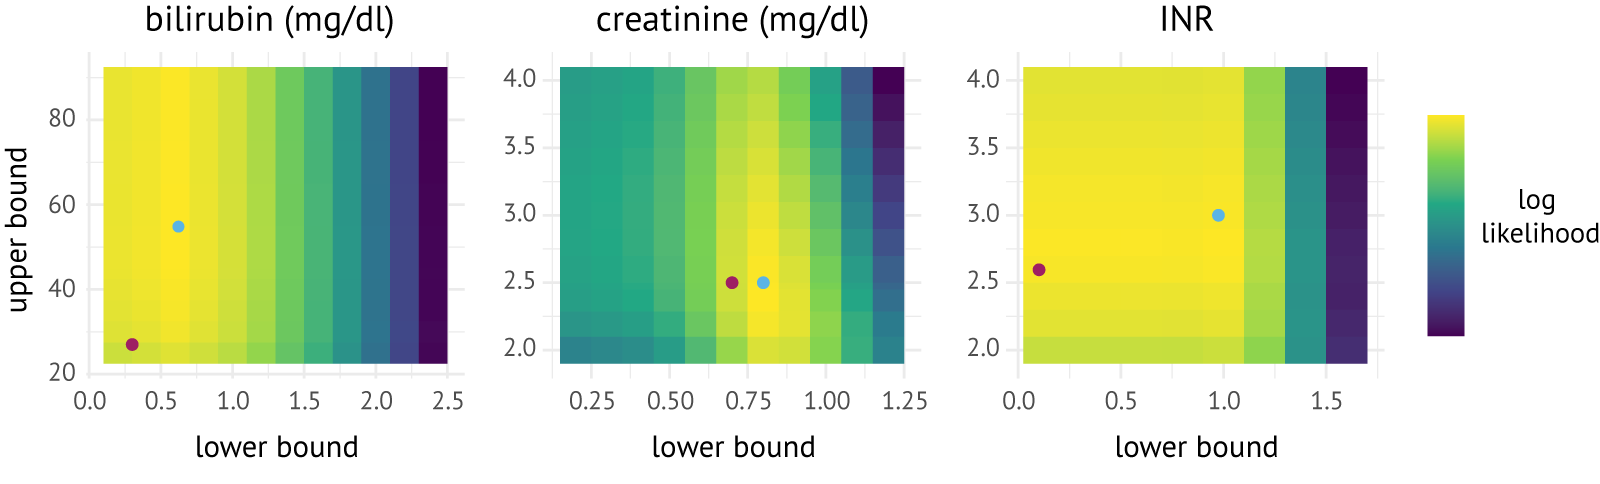
\includegraphics[width=1\linewidth]{figures/ch3//fig_ll} 

}

\caption{Heatmaps of the log-likelihood values for combinations of lower and upper bounds for serum bilirubin (mg/dl), serum creatinine (mg/dl), and the INR. Blue dots represent the optimal caps in the development data; purple dots represent the caps derived for ReMELD.}\label{fig:ch3sfig3}
\end{figure}

\FloatBarrier

\subsubsection{Coefficients revised from registration}\label{coefficients-revised-from-registration}

Panel A of Table \ref{tab:ch3tab2} shows MELD coefficients revised \emph{``from
registration''}. The first column shows that parameter estimates are
jointly not significantly different from 0
(\(\chi_{3}^{2}\) = 4.1,p = 0.25) when using ReMELD's prognostic
index as an offset. The insignificance of these estimates confirms
that ReMELD adequately predicts 90-day mortality \emph{``from registration''} for all cirrhotic
patients. IPCW changes the biomarker
coefficients only slightly (by less than a standard error).

\subsubsection{Coefficients revised from cross-section}\label{coefficients-revised-from-cross-section}

Panel B of Table \ref{tab:ch3tab2} shows MELD coefficients revised \emph{``from
cross-section''}. The first column shows that coefficients are jointly
significantly different from 0 with ReMELD used as an offset
(\(\chi_{3}^{2}\) = 801,p \textless{} 0.001). Hence, ReMELD does not adequately
predict 90-day mortality from cross-section. Estimated coefficients
suggest ReMELD underestimates the effect of creatinine
(\(z\)= 5.2, p \textless{} 0.001) and bilirubin (\(z\) = 6.1, p \textless{} 0.001), but not
the INR (\(z = 0.3,p = 0.76\)). IPCW appears to increase MELD
biomarker coefficients slightly (by less than a standard deviation).

Table \ref{tab:ch3tab2relweights} shows the relative weights put on the MELD
components by the equation revised from cross-section with IPCW.
These weights, originally defined by Sharma et al. \citep{sharmaReweightingModelEndStage2008},
quantify the increase in MELD score resulting from a one-standard deviation increase
in a given biomarker, relative to a one-standard deviation increase in all biomarkers.
These weights also show that the refitted equation puts more weight on bilirubin (41\%)
than UNOS-MELD (36\%) and ReMELD (37\%), and puts less weight on the INR
(28\% vs.~32\% for UNOS-MELD and 34\% for ReMELD).

\begingroup
\setlength{\aboverulesep}{0.2ex}
\setlength{\belowrulesep}{0.3ex}

\begin{table}[h]
\caption{Comparison of MELD coefficients for different model fits from registration (panel A) and “from cross-section” (panel B), for (1) revision with ReMELD's prognostic index as an offset, (2) revision without the offset, and (3) revision with IPCW.}
\label{tab:ch3tab2}
\centering
\resizebox{0.9\ifdim\width>\linewidth\linewidth\else\width\fi}{!}{%

\begin{tabular}{llll}

\multicolumn{4}{l}{panel A - from registration} \\
\cmidrule(l{3pt}r{3pt}){1-4}
  & (1) ReMELD offset & (2) refitted, no IPCW & (3) refitted, IPCW\\
\midrule
ln(bilirubin (mg/dL)) & 0.03 (0.05) & 0.69 (0.05) & 0.73 (0.06)\\
\cmidrule{1-4}
ln(creatinine$^1$ (mg/dL)) & 0.10 (0.09) & 1.62 (0.01) & 1.61 (0.12)\\
\cmidrule{1-4}
ln(INR) & 0.12 (0.17) & 2.02 (0.17) & 2.19 (0.21)\\
\cmidrule{1-4}
biweekly dialysis &  & 1.85 (0.12) & 1.73 (0.13)\\
\cmidrule{1-4}
LR Test & 4.1 (df = 3) & 1482 (df = 4) & 1883 (df = 4)\\
[0.5cm]
\multicolumn{4}{l}{panel B - from cross-section} \\
\cmidrule(l{3pt}r{3pt}){1-4}
  & (1) ReMELD offset & (2) refitted, no IPCW & (3) refitted, IPCW\\
\midrule
ln(bilirubin (mg/dl)) & 0.22 (0.04) & 0.92 (0.04) & 0.97 (0.04)\\
\cmidrule{1-4}
ln(creatinine$^1$ (mg/dl)) & 0.40 (0.08) & 2.07 (0.08) & 2.15 (0.08)\\
\cmidrule{1-4}
ln(INR) & 0.04 (0.13) & 2.06 (0.13) & 2.22 (0.15)\\
\cmidrule{1-4}
biweekly dialysis &  & 1.87 (0.12) & 1.86 (0.12)\\
\cmidrule{1-4}
LR Test & 801 (df = 3) & 22 197 (df = 4) & 26 933 (df = 4)\\
\bottomrule
\end{tabular}
}
\parbox{\textwidth}{\footnotesize \smallskip $\qquad^1$ set to 1.0 mg/dl in case of biweekly dialysis}
\end{table}

\endgroup

\begin{table}[!h]
\centering
\caption{\label{tab:ch3tab2relweights}Relative weights put on bilirubin, creatinine and INR by UNOS-MELD, ReMELD and DynReMELD. Relative weights were calculated $w_{i} = \frac{\beta_{i}\text{SD}_{i}}{\sum_{j}^{}{\beta_{j}\text{SD}_{j}}}$, where $\beta_{i}$ is the coefficient on biomarker $i$ and $\text{SD}_{i}$ its standard deviation in the development cohort.}
\centering
\resizebox{\ifdim\width>\linewidth\linewidth\else\width\fi}{!}{
\fontsize{10}{12}\selectfont
\begin{tabular}[t]{llccl}
\toprule
biomarker & standard deviation & UNOS-MELD & ReMELD & DynReMELD\\
\midrule
bilirubin (mg/dl) & 0.85 & 0.36 & 0.37 & 0.41\\
\cmidrule{1-5}
creatinine (mg/dl) & 0.29 & 0.32 & 0.29 & 0.31\\
\cmidrule{1-5}
INR & 0.26 & 0.32 & 0.34 & 0.28\\
\bottomrule
\end{tabular}}
\end{table}

\subsection{Definition of the DynReMELD score}\label{definition-of-the-dynremeld-score}

Quantile matching of UNOS-MELD to the linear predictor revised \emph{``from
cross-section''} with IPCW (Table \ref{tab:ch3tab2}, panel B) yielded the following
equation for \emph{DynReMELD:}
\[
4.14 \ln(\text{bilirubin}) + 9.12 \ln(\text{creatinine}) + 9.42 \ln(\text{INR}) + 8.50
\]
with creatinine bounded between 0.8 and 2.5 mg/dl, bilirubin between 0.6 and 55 mg/dl, and
the INR between 1.0 and 3.0. We calculate DynReMELD scores by setting
creatinine to the upper cap (2.5 mg/dl) for patients on dialysis. This choice
was made to keep DynReMELD in line with existing clinical implementations of
MELD, and is relatively harmless because the creatinine level required
to attain the same priority as biweekly dialysis is
\(\exp\left( \frac{1.86}{2.15} \right)\  \approx 2.4\ \)mg/dl (Table \ref{tab:ch3tab2},
Panel B, third column).

\FloatBarrier

\subsection{Predictive performance}\label{predictive-performance}

Table \ref{tab:ch3tab3} shows estimates of Gerd's c-index for UNOS-MELD, ReMELD
and DynReMELD, for (a) predicting 90-day waiting list survival from listing
based on biomarkers reported at listing, and (b) predicting 90-day
waiting list survival from calendar-time cross-sections based on the biomarkers
that were last reported for the candidate. The first panel shows c-indices evaluated for predicting 90-day waiting list
survival from listing based on biomarkers reported at listing for
UNOS-MELD, ReMELD and DynReMELD. Point estimates appear to slightly
favor DynReMELD, but bootstrapped pairwise differences are not
statistically significant. The second panel shows that DynReMELD
outperforms UNOS-MELD and ReMELD when predicting 90-day waiting list
survival based on candidates' last reported biomarkers, with DynReMELD
attaining higher c-indices (p \textless{} 0.001) in both development and
validation cohorts. In the validation cohort, the c-index of DynReMELD
(0.7895) is approximately 0.0040 higher than UNOS-MELD (0.7855), and
0.0015 higher than ReMELD (0.7879).

\FloatBarrier

\begingroup
\setlength{\aboverulesep}{0.2ex}
\setlength{\belowrulesep}{0.3ex}

\begin{table}[!h]
\centering
\caption{\label{tab:ch3tab3}C-indices at 90 days after listing with bootstrapped standard errors shown in brackets.}
\centering
\fontsize{10}{12}\selectfont
\begin{tabular}[t]{lll}
\toprule
score & development & validation\\
\midrule
\addlinespace[0.3em]
\multicolumn{3}{l}{\textbf{time-until-death from listing, based on biomarkers at listing}}\\
\hspace{1em}UNOS-MELD & 0.8494 (0.008) & 0.8637 (0.011)\\
\hspace{1em}ReMELD & 0.8503 (0.008) & 0.8623 (0.011)\\
\hspace{1em}DynReMELD & 0.8523$^{\dagger}$ (0.008) & 0.8641 (0.011)\\
\addlinespace[0.3em]
\multicolumn{3}{l}{\textbf{\makecell[l]{remaining time-until-death from cross-sections, based on \\ last reported biomarkers}}}\\
\hspace{1em}UNOS-MELD & 0.8099 (0.002) & 0.7855 (0.004)\\
\hspace{1em}ReMELD & 0.8203$^{***}$ (0.002) & 0.7879 (0.004)\\
\hspace{1em}DynReMELD & 0.8217$^{***}$$^{\dagger\dagger\dagger}$ (0.002) & 0.7895$^{***}$$^{\dagger\dagger}$ (0.004)\\
\bottomrule
\multicolumn{3}{l}{\textsuperscript{} $^{*}$ p < 0.05, $^{**}$ p < 0.01, $^{***}$ p < 0.001, compared to UNOS-MELD}\\
\multicolumn{3}{l}{\textsuperscript{} $^{\dagger}$ p < 0.05, $^{\dagger\dagger}$ p < 0.01, $^{\dagger\dagger\dagger}$ p < 0.001, compared to ReMELD}\\
\end{tabular}
\end{table}

\endgroup

\vspace*{-1em}

\subsection{Estimated absolute survival risk per MELD Score}\label{estimated-absolute-survival-risk-per-meld-score}

This section reports absolute 90-day mortality risks for UNOS-MELD and
DynReMELD estimated \emph{``from cross-section''}. The estimation of mortality
risks \emph{``from cross-section''} is complicated by the fact that most
individuals contribute multiple, correlated observations to the Cox
model. In principle, this dependence can be broken by reporting cross-section-specific estimates of 90-day waiting list survival, but such estimates are
imprecise. To partially break the dependence, we chose to estimate
90-day survival on a data set that included, for each reported set of
biomarkers, only the first cross-section where the patient had an active
waiting list status. Table \ref{tab:ch3tab4} shows 90-day
mortality risks estimated in this way.

The table shows that inverse probability censoring weighting increases
estimates of absolute 90-day mortality risks by almost 10 percentage
points. Failing to correct for informative censoring therefore results in
mortality equivalents that understate the counterfactual mortality
risk. This is of interest to Eurotransplant, as these mortality equivalents
are used by Eurotransplant to assign exception points.

Candidates with multiple sets of biomarkers still contribute multiple observations
to estimating 90-day mortality risks \emph{from cross-section}. Dependence between
such observations can bias estimates of the 90-day mortality risks. It is reassuring
that point estimates of 90-day mortality risks \emph{from registration}
(see Table \ref{tab:ch3stab3}) are close to estimates \emph{from
cross-section} (generally less than 5 percentage point differences are
observed).

\begin{table}[!h]
\centering
\caption{\label{tab:ch3tab4}The 90-day mortality equivalents that are used by Eurotransplant, as well as estimates of the 90-day mortality risk per score. These were estimated with Cox models fitted “from cross-section”, with adjustment for the MELD point score.}
\centering
\resizebox{\ifdim\width>\linewidth\linewidth\else\width\fi}{!}{
\fontsize{10}{12}\selectfont
\begin{tabular}[t]{lcccc}
\toprule
\multicolumn{1}{c}{ } & \multicolumn{2}{c}{UNOS-MELD} & \multicolumn{2}{c}{DynReMELD} \\
\cmidrule(l{3pt}r{3pt}){2-3} \cmidrule(l{3pt}r{3pt}){4-5}
score & no IPCW & IPCW & no IPCW & IPCW\\
\midrule
20 & 0.103 [0.098-0.108] & 0.122 [0.117-0.127] & 0.097 [0.092-0.101] & 0.113 [0.108-0.118]\\
22 & 0.149 [0.142-0.155] & 0.179 [0.171-0.186] & 0.145 [0.139-0.151] & 0.173 [0.166-0.180]\\
24 & 0.212 [0.202-0.221] & 0.258 [0.247-0.270] & 0.214 [0.205-0.224] & 0.260 [0.249-0.271]\\
25 & 0.251 [0.239-0.263] & 0.308 [0.294-0.322] & 0.259 [0.247-0.271] & 0.315 [0.301-0.329]\\
26 & 0.297 [0.282-0.311] & 0.365 [0.348-0.382] & 0.310 [0.295-0.325] & 0.379 [0.361-0.396]\\
\addlinespace
28 & 0.407 [0.385-0.428] & 0.498 [0.473-0.522] & 0.435 [0.413-0.457] & 0.529 [0.503-0.553]\\
29 & 0.470 [0.444-0.495] & 0.572 [0.544-0.599] & 0.508 [0.482-0.533] & 0.612 [0.583-0.639]\\
30 & 0.538 [0.508-0.566] & 0.649 [0.617-0.678] & 0.585 [0.555-0.613] & 0.696 [0.664-0.725]\\
31 & 0.609 [0.576-0.640] & 0.725 [0.691-0.755] & 0.664 [0.632-0.694] & 0.777 [0.744-0.805]\\
32 & 0.681 [0.645-0.714] & 0.796 [0.762-0.825] & 0.742 [0.708-0.772] & 0.848 [0.817-0.874]\\
\addlinespace
33 & 0.751 [0.714-0.784] & 0.859 [0.827-0.885] & 0.814 [0.780-0.842] & 0.907 [0.880-0.927]\\
34 & 0.816 [0.780-0.846] & 0.910 [0.883-0.931] & 0.875 [0.845-0.900] & 0.949 [0.929-0.964]\\
35 & 0.872 [0.839-0.899] & 0.949 [0.927-0.964] & 0.925 [0.899-0.943] & 0.977 [0.963-0.985]\\
36 & 0.918 [0.890-0.940] & 0.974 [0.960-0.984] & 0.959 [0.941-0.972] & 0.991 [0.984-0.995]\\
37 & 0.953 [0.930-0.968] & 0.989 [0.980-0.994] & 0.981 [0.969-0.989] & 0.997 [0.994-0.999]\\
\addlinespace
39 & 0.989 [0.979-0.994] & 0.999 [0.997-1.000] & 0.998 [0.995-0.999] & 1.000 [1.000-1.000]\\
40 & 0.996 [0.991-0.998] & 1.000 [0.999-1.000] & 0.999 [0.998-1.000] & 1.000 [1.000-1.000]\\
\bottomrule
\end{tabular}}
\end{table}

\begin{table}[!h]
\centering
\caption{\label{tab:ch3stab3}Estimates of absolute 90-day mortality risks “from registration” and “from cross-section”. Reported risks were estimated without IPCW.}
\centering
\resizebox{\ifdim\width>\linewidth\linewidth\else\width\fi}{!}{
\fontsize{10}{12}\selectfont
\begin{tabular}[t]{rllll}
\toprule
\multicolumn{1}{c}{ } & \multicolumn{2}{c}{UNOS-MELD} & \multicolumn{2}{c}{DynReMELD} \\
\cmidrule(l{3pt}r{3pt}){2-3} \cmidrule(l{3pt}r{3pt}){4-5}
score & from cross-section & from registration & from cross-section & from registration\\
\midrule
20 & 0.103 [0.098-0.108] & 0.136 [0.127-0.144] & 0.097 [0.092-0.101] & 0.125 [0.116-0.132]\\
22 & 0.149 [0.142-0.155] & 0.187 [0.176-0.197] & 0.145 [0.139-0.151] & 0.176 [0.166-0.186]\\
24 & 0.212 [0.202-0.221] & 0.254 [0.240-0.267] & 0.214 [0.205-0.224] & 0.247 [0.233-0.260]\\
26 & 0.297 [0.282-0.311] & 0.339 [0.321-0.356] & 0.310 [0.295-0.325] & 0.339 [0.321-0.356]\\
28 & 0.407 [0.385-0.428] & 0.443 [0.420-0.466] & 0.435 [0.413-0.457] & 0.453 [0.429-0.476]\\
\addlinespace
30 & 0.538 [0.508-0.566] & 0.564 [0.535-0.591] & 0.585 [0.555-0.613] & 0.586 [0.556-0.613]\\
32 & 0.681 [0.645-0.714] & 0.691 [0.657-0.721] & 0.742 [0.708-0.772] & 0.724 [0.690-0.753]\\
34 & 0.816 [0.780-0.846] & 0.810 [0.776-0.839] & 0.875 [0.845-0.900] & 0.847 [0.815-0.873]\\
36 & 0.918 [0.890-0.940] & 0.905 [0.877-0.927] & 0.959 [0.941-0.972] & 0.935 [0.912-0.953]\\
40 & 0.996 [0.991-0.998] & 0.991 [0.983-0.995] & 0.999 [0.998-1.000] & 0.997 [0.993-0.999]\\
\bottomrule
\end{tabular}}
\end{table}

\FloatBarrier

\section{Discussion}\label{discussion}

Prior literature revised the MELD score with liver waiting list candidate data \emph{``from
registration''} (e.g., \citep{kimHyponatremiaMortalityPatients2008a, kimMELD3point0, goudsmitRefittingModelEndstage2020}), which ignores any
MELD biomarker measurements that are reported after registration and any
waiting list death that occurs more than 90 days after registration. We used methodology proposed
by Gong and Schaubel \citep{gongPartlyConditionalEstimation2013} to model waiting list
mortality from calendar-time cross-sections, which can avoid such waste of statistical
information in revising MELD. Moreover, we assessed how revision of MELD
was affected by correction for selection bias by transplantation or delisting with inverse
probability censoring weighting.

We showed that the \emph{``from cross-section''} approach uses waiting list
registry data substantially more efficiently, with the number of
waiting list deaths and MELD scores informing revision of MELD increasing
sevenfold compared to revision \emph{``from registration''}. DynReMELD, the
score obtained by quantile matching UNOS-MELD to the risk equation that
was developed \emph{``from cross-section''} with IPCW, attains significantly higher
c-indices than ReMELD and UNOS-MELD in a geographical validation cohort
for predicting remaining time-until-death based on last reported MELD
biomarkers (p \textless{} 0.001). This is important for Eurotransplant, as
Eurotransplant liver allocation prioritizes candidates based on their
last reported MELD scores and not MELD at listing. In magnitude,
the improvements in c-indices (0.0015 compared to ReMELD, and 0.0040
compared to UNOS-MELD) are comparable to the addition of serum sodium to
ReMELD (approx. delta c-index of 0.0030)
\citep{goudsmitRefittingModelEndstage2020} and the addition of serum albumin to
MELD 3.0 (delta c-index of 0.0028) \citep{kimMELD3point0}. MELD revision from
cross-section with IPCW can thus improve urgency-based risk
stratification. Our results suggest that the improvement is due to
modeling time-remaining-until-death from cross-sections and not IPCW,
as IPCW changed estimated coefficients only slightly.

We believe the main reason why DynReMELD outperforms ReMELD in
geographical validation is that revision \emph{``from cross-section''} uses Eurotransplant
registry data substantially more efficiently than revision \emph{``from
registration''}, as the latter method only uses the MELD biomarkers that were reported
at listing and the first 90 days of waiting list survival. This raises the
question whether revision \emph{``from registration''} cannot also be improved
upon by using available registry data more efficiently. One way of doing
this would be to include MELD biomarkers as time-varying covariates. However,
because MELD biomarkers also increase inherently as part of the death process,
use of biomarkers as time-varying covariates leads to issues of reverse causality. Follow-up data could,
in principle, also be used more efficiently by not restricting revision \emph{``from
registration''} to the first 90 days after listing. However, we found
that this leads to violations of the proportional hazards assumption for
MELD biomarkers.
\newpage
We also assessed how estimates of the 90-day mortality risks are affected
by (a) revision \emph{``from cross-section''} and (b) correcting for dependent
censoring with IPCW. Revision \emph{``from cross-section''} does not
meaningfully change estimated 90-day mortality risks, with risks
estimated \emph{``from cross-section''} differing by less than 5 percent points
from risks estimated \emph{``from registration''}. This means that we do not
find that there are meaningful differences in 90-day mortality risks between
a candidate who reported a particular MELD score at listing and another
one who reported that same score as part of a MELD
recertification. Mitigation of selection bias with IPCW did increase
estimated 90-day waiting list mortality risks for both UNOS-MELD and
DynReMELD by 10 percentage points. Failure to account for informative censoring by transplantation/delisting thus leads to an underestimation of
90-day mortality equivalents, which can be problematic as Eurotransplant uses
these estimates to assign MELD scores for candidates who receive exception points.

Eurotransplant currently consists of 38 liver transplant centers
located in seven European countries. These centers differ structurally in
terms of patient populations, liver transplantation volumes, and willingness to accept
donors of marginal quality. A strength of our study is that we assigned
candidates to either the development or validation cohort based on their
center of listing, which means that the predictive performance of
DynReMELD was evaluated in a cohort independent from the centers on
which the score was developed.

A limitation of our work is that revision of MELD \emph{``from cross-section''}
only uses the last MELD biomarkers reported before the cross-section date.
Eurotransplant
uses these same biomarker measurements for allocation, but they may be outdated
representations of a patient's health status. Alternatively, one could
model the evolution of MELD biomarkers over time with linear mixed
models, and use a best linear unbiased
predictions (BLUP) of biomarkers at every cross-section time. This BLUP
approach was first proposed by Maziarz et al.
\citep{maziarzLongitudinalPredictionTimetoEvent2017} for landmarking, a
statistical technique which bears similarities to Gong and Schaubel's
approach. We did not use a BLUP approach to revise MELD, since irregular
spacing of MELD measurements complicates modeling the biomarker process. Deployment of BLUP models would also be practically challenging for
Eurotransplant. Moreover, MELD scores for patients with significant
90-day mortality risks are rarely outdated as Eurotransplant requires
frequent re-certification of MELD scores for sicker patients. For example,
MELD scores are on average 12 days old at cross-section for candidates with
MELD scores ranging between 20 and 25
(corresponding to a 90-day mortality risk of 10 to 25\%), and 3 days
old for MELD scores greater than 25 (which corresponds to a mortality risk of
25\% or greater).
\newpage
A final limitation of our work is that DynReMELD was based only on
bilirubin, creatinine and the INR, while updated versions of MELD exist that
use additional biomarkers. Future work could focus on revising these UNOS-MELD
alternatives \emph{``from cross-section''}. This was not pursued in this chapter,
because serum sodium and albumin are unavailable in Eurotransplant registry data
for most patients on the liver waiting list.

\FloatBarrier

\chapter{Sex disparity in liver allocation within Eurotransplant}\label{CHsexdisparity}

\chaptermark{Sex disparity in liver allocation}

\vfill

\begin{center}\rule{0.5\linewidth}{0.5pt}\end{center}

\noindent
An article based on this chapter has appeared in \emph{American Journal of Transplantation}, de Ferrante, H.C., De Rosner-van Rosmalen M., Smeulders, B.M.L., Vogelaar, S., Spieksma, F.C.R., 2025, \href{https://doi.org/10.1016/j.ajt.2024.06.018}{10.1016/j.ajt.2024.06.018} \citep{deFerranteSexDisparityLiver2024}

\newpage
\normalsize

\subsubsection*{Abstract}

On Eurotransplant's liver waiting list, females are relatively more likely to
die than males, and they are relatively less likely to be transplanted. With adult
candidates listed for liver transplantation between 2007
and 2019 (n=21,170), we study whether such sex disparity
is inherent to the Model for End-Stage Liver Disease (MELD) scoring system,
or the indirect result of a small candidate body size limiting access to
transplantation. We use Cox proportional hazards models to quantify (i) the
direct effect of sex on waiting list mortality, independent of sex's effect
through MELD scores, and (ii) the direct effect of sex on the transplant rate,
independent of the effect of sex through MELD and candidate body size. We find that
adjusted waiting list mortality hazard ratios for female sex are insignificant
(HR = 1.03, 95\% CI: 0.88--1.20), which means that we lack indications that MELD
systematically underestimates the waiting list mortality rates for females.
Transplant rates are estimated to be 25\% lower for females than for males in unadjusted
analyses (HR = 0.74, 95\% CI: 0.71--0.77), but hazard ratios become insignificant
after adjustment for mediators, most importantly candidate height
and weight (HR = 0.98, 95\% CI: 0.93--1.04). Sex disparity in Eurotransplant
thus appears to be largely a consequence of the lower transplant rates for females,
which are explained by differences in body size between males and females.

\newpage

\normalsize

\section{Introduction}\label{introduction-1}

Prior research has shown that females are disadvantaged
under MELD-based liver allocation compared to males \citep{moylanDisparitiesLiverTransplantation2008, mathurSexBasedDisparitiesLiver2011, laiHeightContributesGender2010, lockeQuantifyingSexBasedDisparities2020a}.
There are two leading
explanations for such sex disparity in MELD-based liver allocation \citep{vernaTimeActionAddress2020}, which we refer to as the \emph{``GFR hypothesis''} and the \emph{``size mismatch hypothesis''}.

The GFR hypothesis proposes that MELD is biased against female candidates because
MELD is based on serum creatinine instead of glomerular filtration rates (GFR).
With the same serum creatinine level, the GFRs of females are lower than the GFRs
of males \citep{cholongitasFemaleLiverTransplant2007}. MELD would therefore systematically
underestimate the 90-day mortality risks for females. The GFR hypothesis has
frequently been invoked to propose alternatives to MELD which replace serum
creatinine with sex-specific estimates
of the glomerular filtration rate \citep{rodriguezPeralvarezDevelopmentValidationGenderEquity2023, myersGenderRenalFunction2011, asraniMELDGRAILNaGlomerularFiltration2020}. These
alternatives award one to three extra points on the MELD scale to female
liver transplant candidates \citep{vernaTimeActionAddress2020, waltercostaRevisingMELDScore2023, cholongitasGenderDisparityMELD2011, allenReducedAccessLiver2018}.

The second hypothesis relates to donor-recipient size matching in liver transplantation.
Such size matching is crucial in liver transplantation because
(i) the liver must anatomically fit within the recipient's abdominal cavity,
and (ii) the liver has to meet the candidate's metabolic demands. The size-mismatch
hypothesis suggests that transplant candidates with a smaller stature
-- who are predominantly female -- are disadvantaged in MELD-based liver
allocation because donor-recipient size mismatch would require them to turn down
liver offers more frequently. This size mismatch hypothesis has received less
attention in the literature than the GFR hypothesis. Empirical evidence for
it comes from Lai et al.~(2010), who showed that the lower transplant rates
for females in the United States are largely
explained by differences in candidate height \citep{laiHeightContributesGender2010}.
Further evidence comes from Allen et al.~(2018), who showed with competing risk
analyses that height indirectly explains most of the increased waiting list
deaths observed in female candidates \citep{allenReducedAccessLiver2018}. A 2023
study by Sneiders et al.~on retrospective data from Eurotransplant has also linked
a low body weight to adverse liver waiting list outcomes \citep{Sneiders2023}.

In this chapter, we use causal mediation analysis to study the GFR hypothesis and the size mismatch hypothesis. A first
goal is to study whether there is evidence of a direct effect of sex on the
waiting list mortality rate, independently from MELD, as is implied by the
GFR hypothesis. A second goal is to quantify sex disparities in transplantation
rates, and to assess whether such disparities are mediated by
candidate body size -- as is implied by the size mismatch hypothesis. To address
these research questions, we use retrospective data from Eurotransplant.

\FloatBarrier
\newpage

\section{Materials and methods}\label{materials-and-methods-1}

\subsection{Study population}\label{study-population}

Candidates who were activated on the liver waiting list
between January 1, 2007 and December 31, 2019, were considered for inclusion.
We study sex disparity in two subpopulations. The first subpopulation consists
of candidates with common chronic indications for liver
transplantation. This population was obtained by excluding pediatric candidates
(\textless 16 years), candidates with rare metabolic diseases or rare exceptions
(awarded \textless 15 times per year), those with acute liver failure, and
those waiting for a living donor transplantation, a repeat liver transplantation,
or a multi-organ transplantation. The second subpopulation consists of candidates
with cirrhosis who did not have HCC, which is the patient group
for which MELD was originally developed and validated \citep{kamathModelPredictSurvival2001}.
This population was obtained by additionally excluding patients with exception points,
cholestatic liver disease, polycystic liver disease, and hepatocellular carcinoma.
We refer to this second population as ``non-HCC candidates with cirrhosis''.

\subsection{MELD scores}\label{meld-scores}

Liver allocation in Eurotransplant is based on match-MELD scores, i.e., the
maximum of a candidate's lab-MELD score (UNOS-MELD) and their exception scores.
Exception scores can be obtained for candidates with specific indications
who meet predefined eligibility criteria (standardized exceptions, SEs), or
through case-by-case review from national audit groups (non-standardized
exceptions, NSEs). Granted exceptions award an initial 90-day mortality
equivalent. The awarded mortality equivalents increase with every 90 days
of waiting time for most exceptions. For this study, candidates
with five types of exceptions were included: hepatocellular carcinoma (HCC),
polycystic liver disease, biliary sepsis, primary sclerosing cholangitis,
and NSEs. Other exceptions were excluded and are awarded, on average, less
than 15 times per year. The amount of points awarded for these exceptions varies by
country, and they can be found in the Eurotransplant liver manual \citep{ETLiverMan2025}.

Several alternatives to UNOS-MELD have been proposed, which include MELD-Na,
ReMELD-Na and MELD 3.0. MELD 3.0 adds serum sodium, and was used for
liver allocation by UNOS from January 2016 to July 2023. ReMELD-Na
is a revision of MELD-Na on Eurotransplant registry data \citep{goudsmitRefittingModelEndstage2020}.
MELD 3.0 adds serum sodium, serum albumin and female sex to the MELD formula,
and was adopted for liver allocation by UNOS in July 2023. There are indications that
MELD-Na has exacerbated sex disparity \citep{allenReducedAccessLiver2018}, while MELD
3.0 aims to rectify sex disparity by explicitly awarding points for female sex
\citep{kimMELD3point0}. This motivated us to also quantify sex disparity in mortality rates
for these three alternative scores.

Serum sodium and serum albumin are required to calculate these three MELD
alternatives. A problem is that values for these biomarkers are missing for
most candidates, as they were voluntarily reportable in Eurotransplant in the
study period. In this
chapter, main analyses for MELD-Na, ReMELD-Na and MELD 3.0 are done on subgroups
for whom the required biomarkers were available at listing (i.e., complete case analysis).
We compare this with multiple imputation (MI) as a sensitivity check.

\subsection{Statistical analyses}\label{statistical-analyses}

Mediation analysis is used to (i) quantify the total and the controlled direct
effect of sex on transplant rates (Section \ref{CHmediationtxp}),
and (ii) to quantify the controlled direct effect of candidate sex on the
waiting list mortality rate, independent of MELD (Section \ref{CHmediationmrt}).
For both analyses, directed acyclic graphs (DAGs) were constructed to guide
our modeling strategy and communicate visually our causal assumptions
\citep{lipskyCausalDirectedAcyclic2022}.

\subsubsection{Mediation analysis for the transplant rate}\label{CHmediationtxp}

The left-hand side of Figure \ref{fig:ch4fig1} shows the DAG for transplantation
analyses. In this model, sex is the exposure and
transplantation (TXP) is the outcome. Both a candidate's MELD score and their
body size mediate the relation between sex and transplantation. MELD is a
mediator as the GFR hypothesis suggests that sex affects MELD and
MELD affects a candidate's transplantation rate. Body size acts as a mediator,
because sex influences body size, and because the size mismatch hypothesis
suggests that a small body size limits a candidate's access to transplantation.

To identify the controlled direct effect of sex on transplantation, all back-door
paths from sex to transplantation must be blocked. Adjusting for MELD and body
size is not sufficient to block these paths: conditioning on the mediators
(MELD or body size) opens up other back-door paths via U1- and U2-type variables,
which are common causes of MELD and transplantation, and body size and transplantation,
respectively (see Figure \ref{fig:ch4fig1}). To block these back-door paths,
we also have to adjust for these common causes. Common causes of MELD and
the candidate's transplant rate, i.e.~U1-type variables, are whether the candidate
receives biweekly dialysis, their exception score, their age, and
their disease group, which affect both a candidate's MELD score and their center's
willingness to accept and transplant a liver offer. Common causes of body size
and the transplant rate, i.e.~U2-type variables, are candidate frailty
(which is associated with a lower weight and can be a contraindication for
transplantation), as well as diabetes (which is
associated with a higher weight, and which is also a possible contraindication).

\begin{figure}[ht]

{\centering 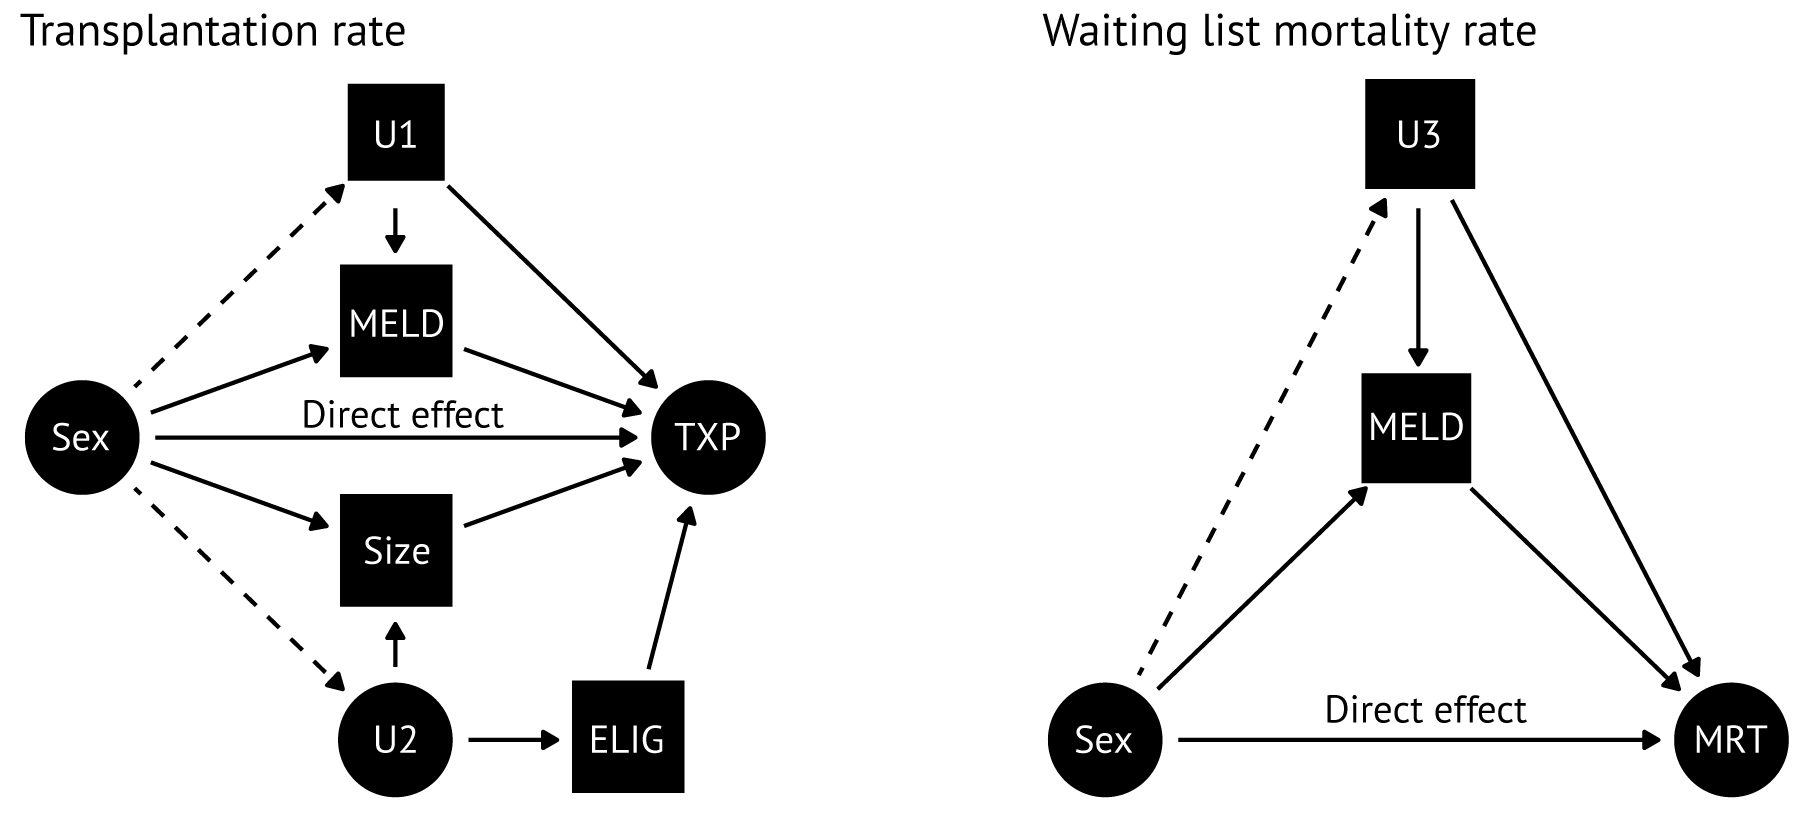
\includegraphics[width=1\linewidth]{figures/ch4/fig1_plot_causal_models} 

}

\caption{Directed acyclic graphs (DAGs) for mediation analyses of the effect of sex on transplantation (TXP, left) and the effect of sex on pre-transplant mortality rates (MRT, right). Squares indicate the minimal sufficient adjustment set required to identify the controlled direct effect of sex on the outcome. U1, U2, and U3 represent common causes of the mediator-outcome relations. U1-, U2-, and U3-variables are post-exposure confounders
  if the dotted arrows are present. We note that the direct effect of sex on transplantation and/or MELD can still be identified, regardless of whether U1, U2 and U3 are regular confounders or post-exposure confounders.}\label{fig:ch4fig1}
\end{figure}

\FloatBarrier

By controlling for MELD, size, U1- and U2-type variables, we could in principle
identify the controlled direct effect of sex on the transplant rate. Unfortunately,
this adjustment strategy is not feasible in our setting, as frailty and diabetes
(U2-type variables) are not reported to Eurotransplant. Instead, we assume that
these U2-type variables only affect the transplant rate via candidate eligiblity
for transplantation (ELIG). With this additional assumption, we can identify
the controlled direct effect of sex on transplantation by adjusting for U1,
MELD, size, and ELIG.

We consider this assumption plausible for two reasons. Firstly, our analysis
implicitly adjusts for candidate eligibility as our cohort is restricted to
candidates who were actually activated on the liver waiting list. Such waiting
list activation represents a strong signal that the candidate is deemed fit
enough for transplantation by their center, as frail or overweight candidates
would be required to improve their health status before waiting list activation
(for example in consultation with a dietitian). Secondly, we can adjust for
temporarily non-transplantability of a candidate as a time-varying variable
in our analyses. Centers use such temporary non-transplantability to indicate
that they temporarily do not want to receive offers for a specific candidate,
for instance because of a poor health status.

\newpage

To estimate the effects of sex on transplant rates, we use Cox proportional
hazards models which use time since waiting list activation as the timescale.
For quantification of the direct effect of sex on the transplant rate, we adjust
for match-MELD, body size (height, weight, or both), and U1-type variables
(dialysis, type exception received, candidate age, and disease group / cirrhosis
etiology through stratification), and temporarily non-transplantability of
the candidate (time-varying variable). In our analyses, we further
adjust for pure predictors of the transplantation
rate (country of listing through stratification, blood group, time spent non-transplantable).
The following variables are time-varying: primary disease group,
non-transplantable (NT) status, time spent NT (separately for too good / too bad / other), the match
MELD, type of exception, and receival of dialysis twice within a week before the last
reported lab-MELD score. Continuous variables are adjusted for with natural
cubic spline transformations with 4 degrees of freedom.

Three sensitivity checks are done. The first is to examine whether
there are sex-height and sex-weight interactions. This sensitivity check is motivated by
findings by Allen et al., who reported that the relation between candidate
height and the relative transplant rate differs significantly by candidate sex
in the United States \citep{allenReducedAccessLiver2018}. The other sensitivity
checks are related to Eurotransplant-specific allocation mechanisms that give physicians freedom to
choose candidates for transplantation. Two such mechanisms are allocation
through extended allocation (15\% of placements) and competitive rescue
allocation (10\% of placements), which Eurotransplant jointly refers to as \emph{non-standard}
allocation mechanisms. To rule out that sex disparities
are the result of physician preferences in non-standard allocation, we
repeat analyses with transplantation through standard allocation as
the outcome (our second sensitivity check). Another mechanism that
allows centers to freely choose a living waiting list candidate for transplantation
are center offers. As the third sensitivity check, we repeat the analysis on candidates listed in
countries without center offers (Germany and the Netherlands).

\newpage
\#\#\#\# Mediation analyses for the waiting list mortality rate \{\#CHmediationmrt\}

The right-hand side of Figure \ref{fig:ch4fig1} shows the DAG for mortality analyses.
Sex is the exposure, and waiting list mortality is the outcome. MELD is a mediator
of sex's effect on mortality, as the GFR hypothesis suggests that a candidate's
sex affects their MELD score. The GFR hypothesis suggests that females face a
systematically higher mortality rate than males, when at the same MELD score.
This suggests that there is a controlled direct effect of sex on the mortality rate,
not mediated by lab-MELD. To identify this effect in the DAG presented in Figure
\ref{fig:ch4fig1}, we must control for lab-MELD, and (post-exposure)
confounders of the relation between lab-MELD and mortality (U3-type variables).

We estimate the controlled direct effect of sex on mortality, with
adjustment for four definitions of the lab-MELD score: UNOS-MELD, MELD-Na,
ReMELD-Na, and MELD 3.0. To estimate these controlled direct effects,
we adjust for a candidate's lab-MELD score, and several common causes of the
lab-MELD score and mortality: the candidate's disease group through stratification,
biweekly dialysis, candidate age, and the type of exception a candidate has
received. We also stratify models by the candidate's country of listing.
Whether the candidate has died on the waiting list death is used as the outcome.
Candidates who died within 90 days of delisting are treated as a waiting list
death. Candidates still waiting 90 days after waiting list activation are censored
administratively. Candidates transplanted or delisted within 90 days of listing
are also censored.

Several sensitivity checks are conducted. Firstly, we repeat the analyses in datasets
where serum sodium and albumin at listing were imputed with multiple imputation (MI).
Secondly, we compare to using death / removed unfit as a combined outcome.
Thirdly, Lai et al.~reported that sex
disparity increased with renal dysfunction \citep{laiHeightContributesGender2010},
motivating us to repeat the analyses
in candidates with high MELD scores (MELD ≥18, 31\% of candidates) and
elevated creatinine (≥1.0 mg/dl, 39\% of candidates). Finally, to exclude
that impending waiting list deaths are prevented with center offers,
we repeat the analysis in Dutch and German candidates only.

\subsubsection{Correction for dependent censoring in mortality analyses}\label{correction-for-dependent-censoring-in-mortality-analyses}

The standard Cox PH model assumes that censoring is non-informative, which means
that conditional on covariates, censored candidates have similar expected
survival as non-censored candidates. In our mortality analyses, we also censor
patients at transplantation, while we adjust for a candidate's MELD score reported
at listing. The non-informative censoring assumption would entail that
transplanted candidates and candidates who are not (yet) transplanted
with the same MELD score at listing would face
similar mortality risks if they had remained on the waiting list.
\newpage
This assumption is implausible for the Eurotransplant liver waiting list, as
Eurotransplant ranks candidates by their last reported MELD score and
not MELD at listing. Of the two candidates with the same
MELD score at listing, the candidate with a higher last reported MELD score would
thus face a higher mortality and higher transplant rate. In expectation,
transplanted candidates therefore have lower without-transplant survival than
non-transplanted candidates, which violates the non-informative censoring
assumption.

One can correct for this bias with inverse probability censoring weighting (IPCW),
as was previously applied in studying sex disparity by Wood et al. \citep{woodCorrectingSexDisparity2021}. In this chapter, we use statistical methodology
developed by Gong and Schaubel to account for selection bias by transplantation \citep{gongEstimatingAverageTreatment2017}. Details on this procedure are included
in Appendix \ref{APPipcw}. A sensitivity check is included to assess how IPCW
affects estimates of the direct effects of sex.

\subsubsection{Multiple imputation}\label{multiple-imputation}

Multiple imputation is used as a sensitivity check in quantifying the direct
effect of sex on the waiting list mortality rate. For this, we used multiple
imputation with chained equations (MICE) to impute serum sodium and serum albumin values at
listing using predictive mean matching, constructing M = 10 completed datasets.
After imputing serum sodium and albumin, MELD-Na, MELD 3.0, and ReMELD-Na were
calculated using the imputed values. We included the event indicator
and estimated baseline cumulative hazard in the imputation procedure, as
recommended by White et al. \citep{whiteMultipleImputationUsing2011}.
MICE yields unbiased estimation of regression coefficients under a missing at
random (MAR) assumption. This assumption would be violated if a candidate's actual serum sodium or albumin value influenced whether that value was available at Eurotransplant. Such a violation is implausible in our setting, as missingness arises almost entirely from center-level policies: some centers always report serum sodium and albumin to Eurotransplant, while other centers never report these biomarkers. The availability of these laboratory values is not determined by the candidate's true biomarker level, but exclusively by their center's reporting policy for serum sodium and albumin.

\section{Results}\label{results-1}

This study considered 31,756 candidate listings for inclusion
(see Figure \ref{fig:ch4fig2}). From these registrations, we excluded pediatric candidates (n=1,652), listings for repeat liver transplantation (n=3,865) or multi-organ transplantation (n=1,523),
candidates with acute liver failure or a High Urgency (HU) status (n=1,753), and candidates
with rare metabolic diseases or rare exceptions (n=755). The main cohort
consisted of 21,188 listings belonging to 21,170 candidates.

\begin{figure}[ht]

{\centering 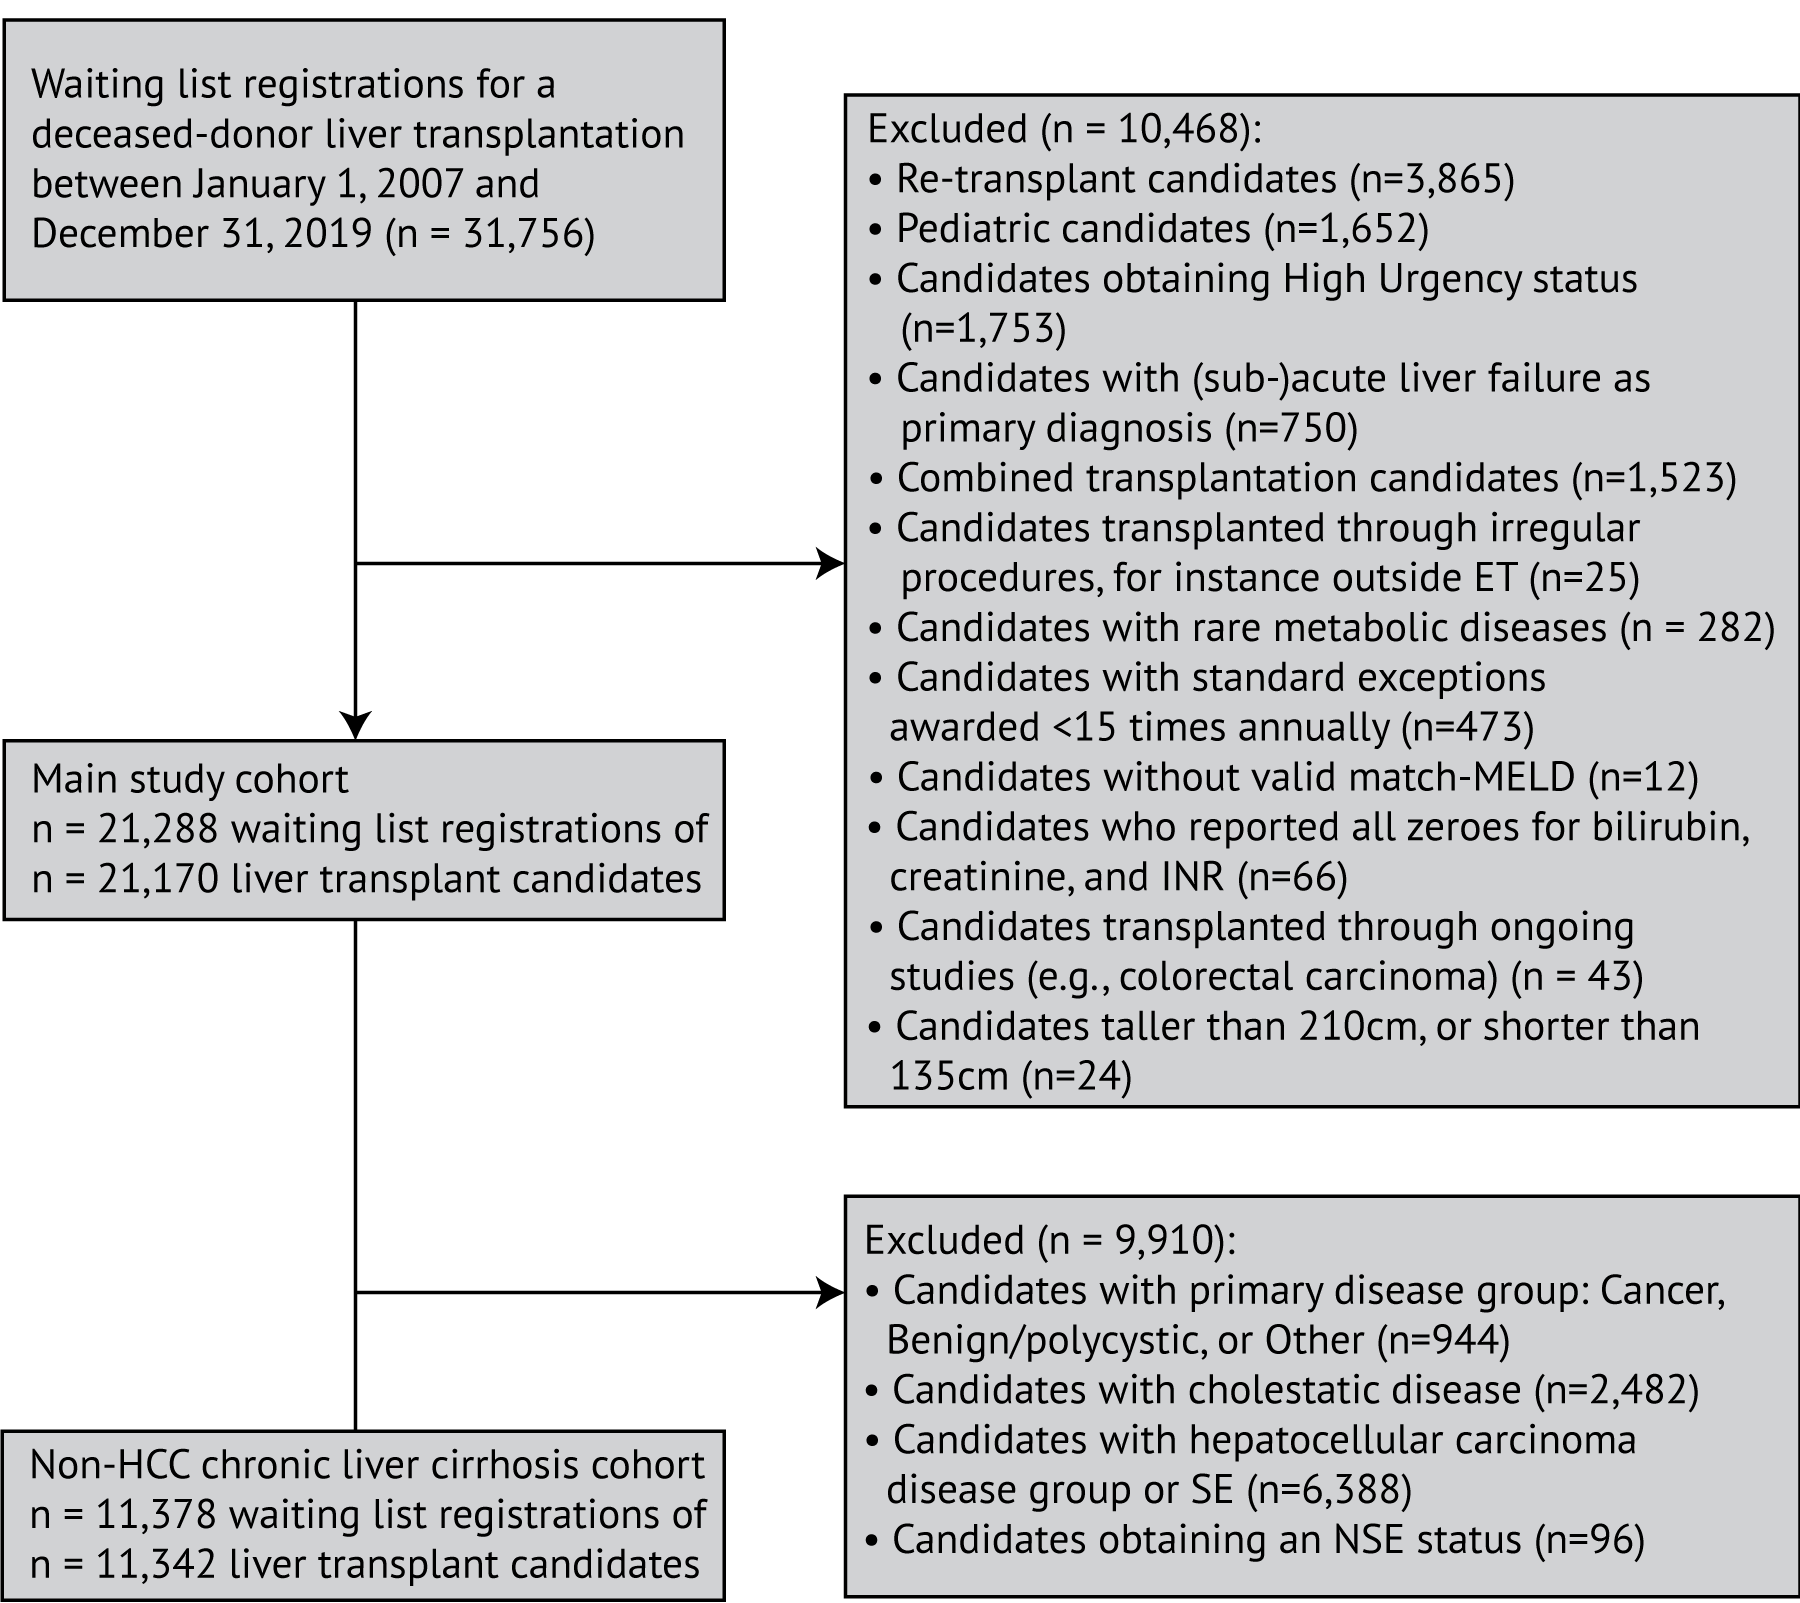
\includegraphics[width=0.95\linewidth]{figures/ch4/fig2_flow_diagram} 

}

\caption{Flow diagram for how the main study cohort and the subpopulation of non-HCC candidates with cirrhosis were selected from all candidates listed between January 1, 2007 and December 31, 2019.}\label{fig:ch4fig2}
\end{figure}

\FloatBarrier

Table \ref{tab:ch4tab1} describes the baseline characteristics of candidates included in the
main cohort, of whom 6,597 (31\%) are female and 14,573 (69\%) are male. We
use standardized mean differences (SMD) to compare the distributions of baseline
variables across sexes, with SMD greater than 0.10 interpreted as meaningful imbalance.
On average, females are 2 years younger (SMD: 0.19),
12 cm shorter (SMD: 1.8) and 15 kg lighter (SMD: 1.0) than males. Females also
have on average 0.13 mg/dl lower serum creatinine at listing (SMD: 0.20) and
0.6 mg/dl higher bilirubin (SMD: 0.08). Despite these
differences, the calculated UNOS-MELD scores are similar
between the sexes (SMD: 0.00).
There is sex imbalance in etiologies of end-stage liver disease (SMD: 0.49), with
notably fewer females listed with HCC (11.8\% of females compared to 21\% of males). Relatively fewer females receive
exception points (SMD: 0.32).

\begingroup
\setlength{\aboverulesep}{0.2ex}
\setlength{\belowrulesep}{0.3ex}

\begin{table}[!h]
\centering
\caption{\label{tab:ch4tab1}Baseline characteristics of primary liver transplant candidates included in this study. For candidates with multiple listings only the first listing was used (n=118).}
\centering
\resizebox{\ifdim\width>\linewidth\linewidth\else\width\fi}{!}{
\fontsize{10}{12}\selectfont
\begin{tabular}[t]{llccl}
\toprule
variable & level & females (n=6,597) & males (n=14,573) & SMD\\
\midrule
 & cirrhosis & 3,771 (57.2\%) & 7,976 (54.7\%) & 0.487\\
\cmidrule{2-5}
 & benign tumor or PLD & 306 (4.6\%) & 62 (0.4\%) & \\
\cmidrule{2-5}
 & cancer & 129 (2.0\%) & 172 (1.2\%) & \\
\cmidrule{2-5}
 & cholestatic & 1,092 (16.6\%) & 1,350 (9.3\%) & \\
\cmidrule{2-5}
 & HCC & 1,096 (16.6\%) & 4,654 (31.9\%) & \\
\cmidrule{2-5}
 & metabolic & 72 (1.1\%) & 233 (1.6\%) & \\
\cmidrule{2-5}
\multirow{-7}{*}[6\dimexpr\aboverulesep+\belowrulesep+\cmidrulewidth]{\raggedright\arraybackslash disease group} & other & 131 (2.0\%) & 126 (0.9\%) & \\
\cmidrule{1-5}
 & cholestatic & 163 (2.5\%) & 324 (2.2\%) & 0.318\\
\cmidrule{2-5}
 & HCC & 780 (11.8\%) & 3,180 (21.8\%) & \\
\cmidrule{2-5}
 & NSE & 115 (1.7\%) & 168 (1.2\%) & \\
\cmidrule{2-5}
 & PLD & 127 (1.9\%) & 24 (0.2\%) & \\
\cmidrule{2-5}
\multirow{-5}{*}[4\dimexpr\aboverulesep+\belowrulesep+\cmidrulewidth]{\raggedright\arraybackslash exception at listing} & none & 5,412 (82.0\%) & 10,877 (74.6\%) & \\
\cmidrule{1-5}
match-MELD & mean [Q1-Q3] & 16 [10-20] & 16 [10-20] & 0.002\\
\cmidrule{1-5}
lab-MELD & mean [Q1-Q3] & 15.8 [9.7-19.6] & 15.7 [10.2-18.8] & 0.025\\
\cmidrule{1-5}
MELD-Na & mean [Q1-Q3] & 17.4 [11.0-22.4] & 17.4 [11.0-22.0] & 0.007\\
\cmidrule{1-5}
ReMELD-Na & mean [Q1-Q3] & 14.9 [9.3-19.4] & 15.3 [10.3-19.3] & 0.058\\
\cmidrule{1-5}
bilirubin (mg/dl) & mean [Q1-Q3] & 5.51 [1.10-6.08] & 4.87 [1.17-4.66] & 0.083\\
\cmidrule{1-5}
creatinine (mg/dl) & mean [Q1-Q3] & 1.00 [0.67-1.10] & 1.13 [0.78-1.22] & 0.200\\
\cmidrule{1-5}
INR & mean [Q1-Q3] & 1.49 [1.13-1.60] & 1.47 [1.17-1.60] & 0.038\\
\cmidrule{1-5}
 & mean [Q1-Q3] & 137 [134-140] & 136 [134-140] & 0.044\\
\cmidrule{2-5}
\multirow{-2}{*}[1\dimexpr\aboverulesep+\belowrulesep+\cmidrulewidth]{\raggedright\arraybackslash serum sodium (mmol/l)} & missing & 4,238 (64.2\%) & 9,118 (62.6\%) & \\
\cmidrule{1-5}
 & mean [Q1-Q3] & 3.3 [2.9-3.8] & 3.3 [2.8-3.7] & 0.073\\
\cmidrule{2-5}
\multirow{-2}{*}[1\dimexpr\aboverulesep+\belowrulesep+\cmidrulewidth]{\raggedright\arraybackslash serum albumin (g/dl)} & missing & 5,219 (79.1\%) & 11,502 (78.9\%) & \\
\cmidrule{1-5}
dialysis twice in the last week &  & 171 (2.6\%) & 332 (2.3\%) & 0.020\\
\cmidrule{1-5}
candidate height (cm) & mean [Q1-Q3] & 165 [160-169] & 177 [172-182] & 1761\\
\cmidrule{1-5}
candidate weight (kg) & mean [Q1-Q3] & 69 [59-77] & 84 [74-94] & 1020\\
\cmidrule{1-5}
age at registration (years) & mean [Q1-Q3] & 53 [47-61] & 55 [50-62] & 0.185\\
\cmidrule{1-5}
 & transplanted & 1,458 (22.1\%) & 4,266 (29.3\%) & \\
\cmidrule{2-5}
 & died & 514 (7.8\%) & 979 (6.7\%) & \\
\cmidrule{2-5}
 & waiting & 4,464 (67.7\%) & 8,927 (61.3\%) & \\
\cmidrule{2-5}
 & censored & 82 (1.2\%) & 159 (1.1\%) & \\
\cmidrule{2-5}
\multirow{-5}{*}[4\dimexpr\aboverulesep+\belowrulesep+\cmidrulewidth]{\raggedright\arraybackslash exit reason (90 days)} & removed & 79 (1.2\%) & 242 (1.7\%) & \\
\cmidrule{1-5}
 & transplanted & 2,764 (41.9\%) & 7,844 (53.8\%) & \\
\cmidrule{2-5}
 & died & 904 (13.7\%) & 1,755 (12.0\%) & \\
\cmidrule{2-5}
 & waiting & 2,381 (36.1\%) & 3,765 (25.8\%) & \\
\cmidrule{2-5}
 & censored & 272 (4.1\%) & 419 (2.9\%) & \\
\cmidrule{2-5}
\multirow{-5}{*}[4\dimexpr\aboverulesep+\belowrulesep+\cmidrulewidth]{\raggedright\arraybackslash exit reason (1 year)} & removed & 276 (4.2\%) & 790 (5.4\%) & \\
\bottomrule
\end{tabular}}
\parbox{\textwidth}{\footnotesize \smallskip \textbf{Abbreviations: } PLD, polycystic liver disease; HCC, hepatocellular carcinoma; MELD, model for end-stage liver disease; MELD-Na, model for end-stage liver disease sodium; NSE, non-standard exception; ReMELD-Na, refitted MELD-Na for Eurotransplant; SMD, standardized mean difference.}
\end{table}

\endgroup

\FloatBarrier

In terms of outcomes, Table \ref{tab:ch4tab1} shows that relatively fewer females
than males are transplanted 90 days after listing (22\% vs.~29\%), and relatively
more females die within 90 days of listing (7.8\% vs.~6.7\%). This sex disparity
has increased one year after listing, with only 41.9\% of females transplanted compared to
53.8\% of males, and 13.7\% of female candidates having died on the waiting list
compared to 12.0\% of males.

The cohort of non-HCC candidates with cirrhosis (n=11,342) was obtained by excluding
candidates with HCC (n=6,388), non-cirrhotic indications for liver
transplantation (n=3,426) or NSEs (n=96)
(see Figure \ref{fig:ch4fig2}). Baseline characteristics of this subpopulation
are reported in Table \ref{tab:ch4tab1cirrhotic}. Also among
this group, relatively fewer females are transplanted (26\% vs.~32\% of males) and
relatively more females die (10.5\% vs.~9.8\%) within 90 days of listing.

Figure \ref{fig:ch4fig3} shows the distributions of the time spent by candidates on the waiting list
until waiting list exit (death, delisting, or transplantation), separately for exception
and non-exception patients. Whether or not they receive exception points, females
spend approximately 75 more days on the waiting list than males.

\begin{figure}[ht]

{\centering 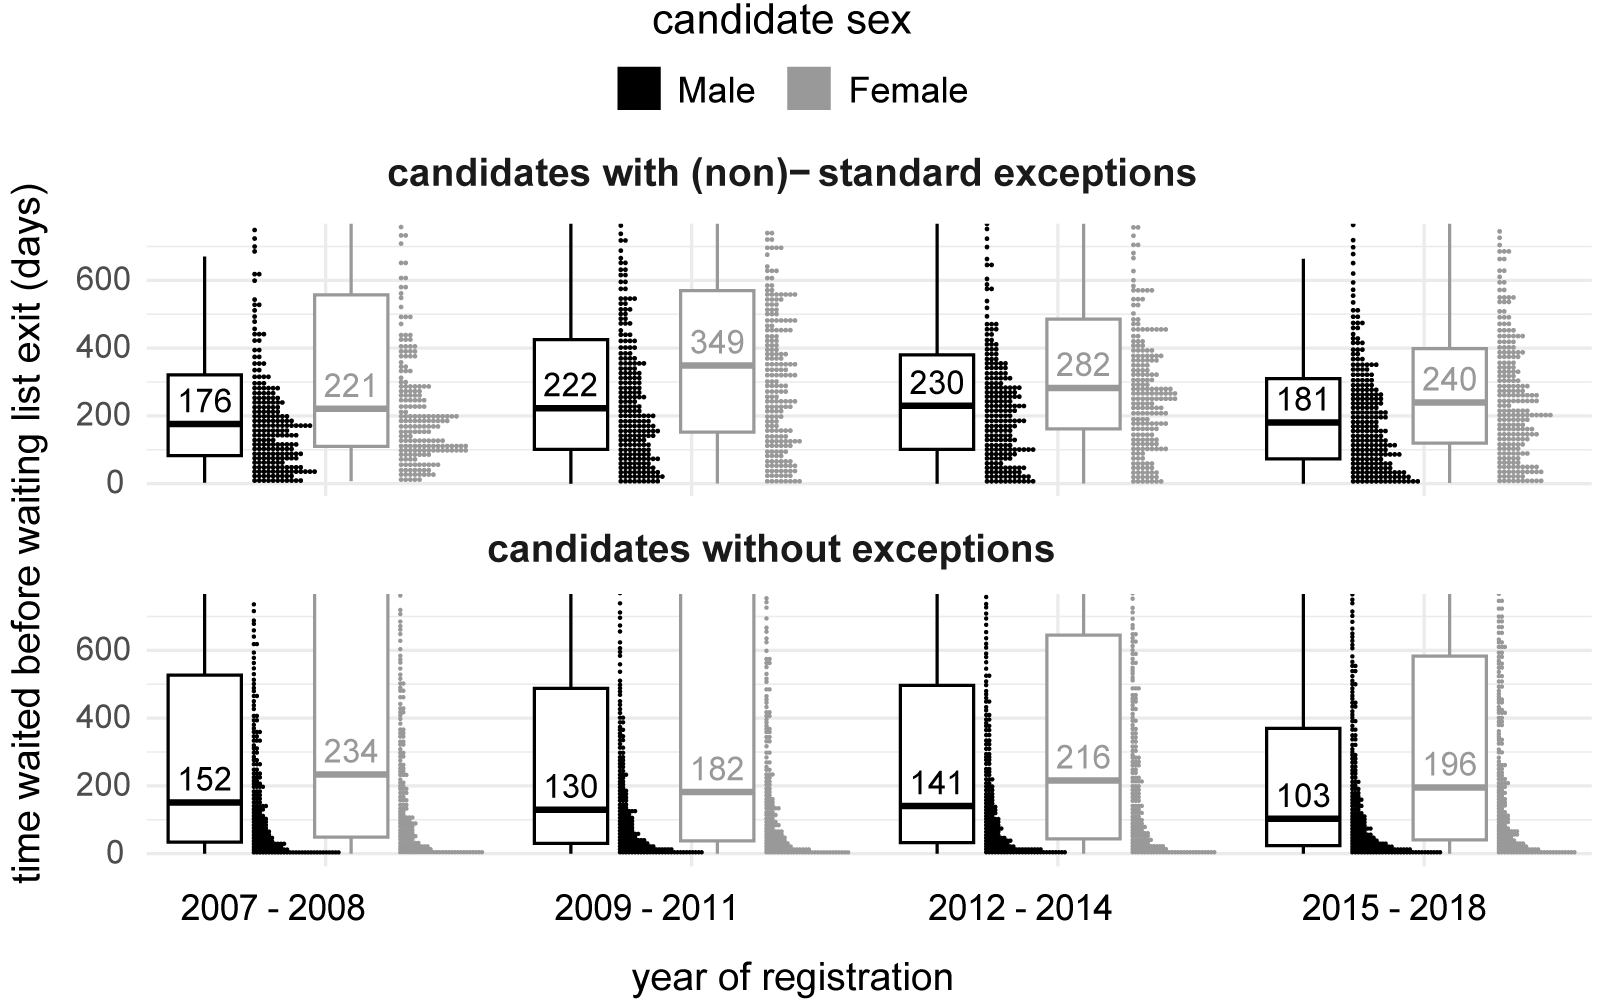
\includegraphics[width=1\linewidth]{figures/ch4/fig3_waittime_at_exit} 

}

\caption{Distributions of the time spent on the waiting list until waiting list exit (transplantation, death, or delisting), by sex and year of waiting list inclusion. The top panel shows waiting times for candidates with (non-)standard exceptions, the bottom panel for candidates without exceptions. Distributions were
  visualized with quantile dotplots, using 250 quantiles. The numbers displayed in the boxplots are the median number of days spent on the waiting list per group.}\label{fig:ch4fig3}
\end{figure}

\FloatBarrier
\newpage
\begingroup
\setlength{\aboverulesep}{0.2ex}
\setlength{\belowrulesep}{0.3ex}

\begin{table}[!h]
\centering
\caption{\label{tab:ch4tab1cirrhotic}Baseline characteristics for the subcohort of non-HCC candidates with cirrhosis.}
\centering
\resizebox{\ifdim\width>\linewidth\linewidth\else\width\fi}{!}{
\fontsize{10}{12}\selectfont
\begin{tabular}[t]{llccl}
\toprule
variable & level & females (n=3,667) & males (n=7,675) & SMD\\
\midrule
 & alcoholic & 1,686 (46.0\%) & 4,547 (59.2\%) & 0.37\\
\cmidrule{2-5}
 & autoimmune/cryptogenic & 933 (25.4\%) & 961 (12.5\%) & \\
\cmidrule{2-5}
 & NAFLD$^a$ & 189 (5.2\%) & 264 (3.4\%) & \\
\cmidrule{2-5}
 & hepatitis B & 166 (4.5\%) & 435 (5.7\%) & \\
\cmidrule{2-5}
 & hepatitis C & 438 (11.9\%) & 870 (11.3\%) & \\
\cmidrule{2-5}
\multirow{-6}{*}[5\dimexpr\aboverulesep+\belowrulesep+\cmidrulewidth]{\raggedright\arraybackslash cirrhosis aetiology} & metabolic/other/unknown & 255 (7.0\%) & 598 (7.8\%) & \\
\cmidrule{1-5}
lab-MELD & mean [Q1-Q3] & 18.5 [12.4-22.3] & 18.5 [13.0-21.9] & 0.005\\
\cmidrule{1-5}
MELD-Na & mean [Q1-Q3] & 19.8 [13.9-24.7] & 20.2 [14.8-24.5] & 0.043\\
\cmidrule{1-5}
ReMELD-Na & mean [Q1-Q3] & 17.2 [12.1-21.6] & 17.9 [13.4-21.7] & 0.100\\
\cmidrule{1-5}
bilirubin (mg/dl) & mean [Q1-Q3] & 6.64 [1.64-7.56] & 6.17 [1.70-6.20] & 0.055\\
\cmidrule{1-5}
creatinine (mg/dl) & mean [Q1-Q3] & 1.12 [0.71-1.26] & 1.26 [0.81-1.40] & 0.182\\
\cmidrule{1-5}
INR & mean [Q1-Q3] & 1.66 [1.28-1.80] & 1.63 [1.30-1.79] & 0.037\\
\cmidrule{1-5}
 & mean [Q1-Q3] & 136 [133-139] & 135 [132-139] & 0.102\\
\cmidrule{2-5}
\multirow{-2}{*}[1\dimexpr\aboverulesep+\belowrulesep+\cmidrulewidth]{\raggedright\arraybackslash serum sodium (mmol/l)} & missing & 2,180 (59.4\%) & 4,398 (57.3\%) & \\
\cmidrule{1-5}
 & mean [Q1-Q3] & 3.2 [2.8-3.6] & 3.2 [2.7-3.6] & 0.099\\
\cmidrule{2-5}
\multirow{-2}{*}[1\dimexpr\aboverulesep+\belowrulesep+\cmidrulewidth]{\raggedright\arraybackslash serum albumin (g/dl)} & missing & 2,697 (73.5\%) & 5,512 (71.8\%) & \\
\cmidrule{1-5}
dialysis twice in last week &  & 137 (3.7\%) & 262 (3.4\%) & 0.017\\
\cmidrule{1-5}
candidate height (cm) & mean [Q1-Q3] & 165 [160-169] & 177 [172-182] & 1809\\
\cmidrule{1-5}
candidate weight (kg) & mean [Q1-Q3] & 69 [59-77] & 85 [74-95] & 0.99\\
\cmidrule{1-5}
age at registration (years) & mean [Q1-Q3] & 54 [48-61] & 55 [49-61] & 0.102\\
\cmidrule{1-5}
 & transplanted & 947 (25.8\%) & 2,458 (32.0\%) & \\
\cmidrule{2-5}
 & died & 380 (10.4\%) & 756 (9.9\%) & \\
\cmidrule{2-5}
 & waiting & 2,272 (62.0\%) & 4,319 (56.3\%) & \\
\cmidrule{2-5}
 & censored & 39 (1.1\%) & 75 (1.0\%) & \\
\cmidrule{2-5}
\multirow{-5}{*}[4\dimexpr\aboverulesep+\belowrulesep+\cmidrulewidth]{\raggedright\arraybackslash exit reason (90 days)} & removed & 29 (0.8\%) & 67 (0.9\%) & \\
\cmidrule{1-5}
 & transplanted & 1,424 (38.8\%) & 3,851 (50.2\%) & \\
\cmidrule{2-5}
 & died & 643 (17.5\%) & 1,290 (16.8\%) & \\
\cmidrule{2-5}
 & waiting & 1,365 (37.2\%) & 2,149 (28.0\%) & \\
\cmidrule{2-5}
 & censored & 126 (3.4\%) & 179 (2.3\%) & \\
\cmidrule{2-5}
\multirow{-5}{*}[4\dimexpr\aboverulesep+\belowrulesep+\cmidrulewidth]{\raggedright\arraybackslash exit reason (1 year)} & removed & 109 (3.0\%) & 206 (2.7\%) & \\
\bottomrule
\end{tabular}}
\parbox{\textwidth}{\footnotesize \smallskip $^a$Many candidates with NAFLD have likely been registered under the autoimmune/cryptogenic disease code, as NAFLD could only be reported via free text during the study period.

\textbf{Abbreviations: } NAFLD, non-alcoholic fatty liver disease; MELD, model for end-stage liver disease; MELD-Na, model for end-stage liver disease sodium; ReMELD-Na, refitted MELD-Na for Eurotransplant; SMD, standardized mean difference.}
\end{table}

\endgroup
\newpage

\subsection{Transplantation analyses}\label{CHrsltsmediationtxp}

Figure \ref{fig:ch4fig4} shows the estimated transplantation hazard ratios (HRs)
for female sex. The unadjusted effect of sex in the full cohort (top panel) suggest that the
transplant rates are approximately 25\% lower for females
(HR = 0.74, 95\% CI: 0.71--0.76). When
adjusting for candidate body size (weight + height) plus confounders of the
mediator-outcome relations, no sex difference in transplant rates is
found (HR = 0.98, 95\% CI: 0.93--1.04). Similar results are found in non-HCC
candidates with cirrhosis (bottom panel), with 22\% lower transplant rates for females in total (HR = 0.78, 95\% CI: 0.74--0.82) but no sex
difference in transplant rates when adjusting for body size,
MELD, and confounders of both mediator-outcome relations (HR = 1.00, 95\% CI: 0.93--1.07).

\begin{figure}[ht]

{\centering 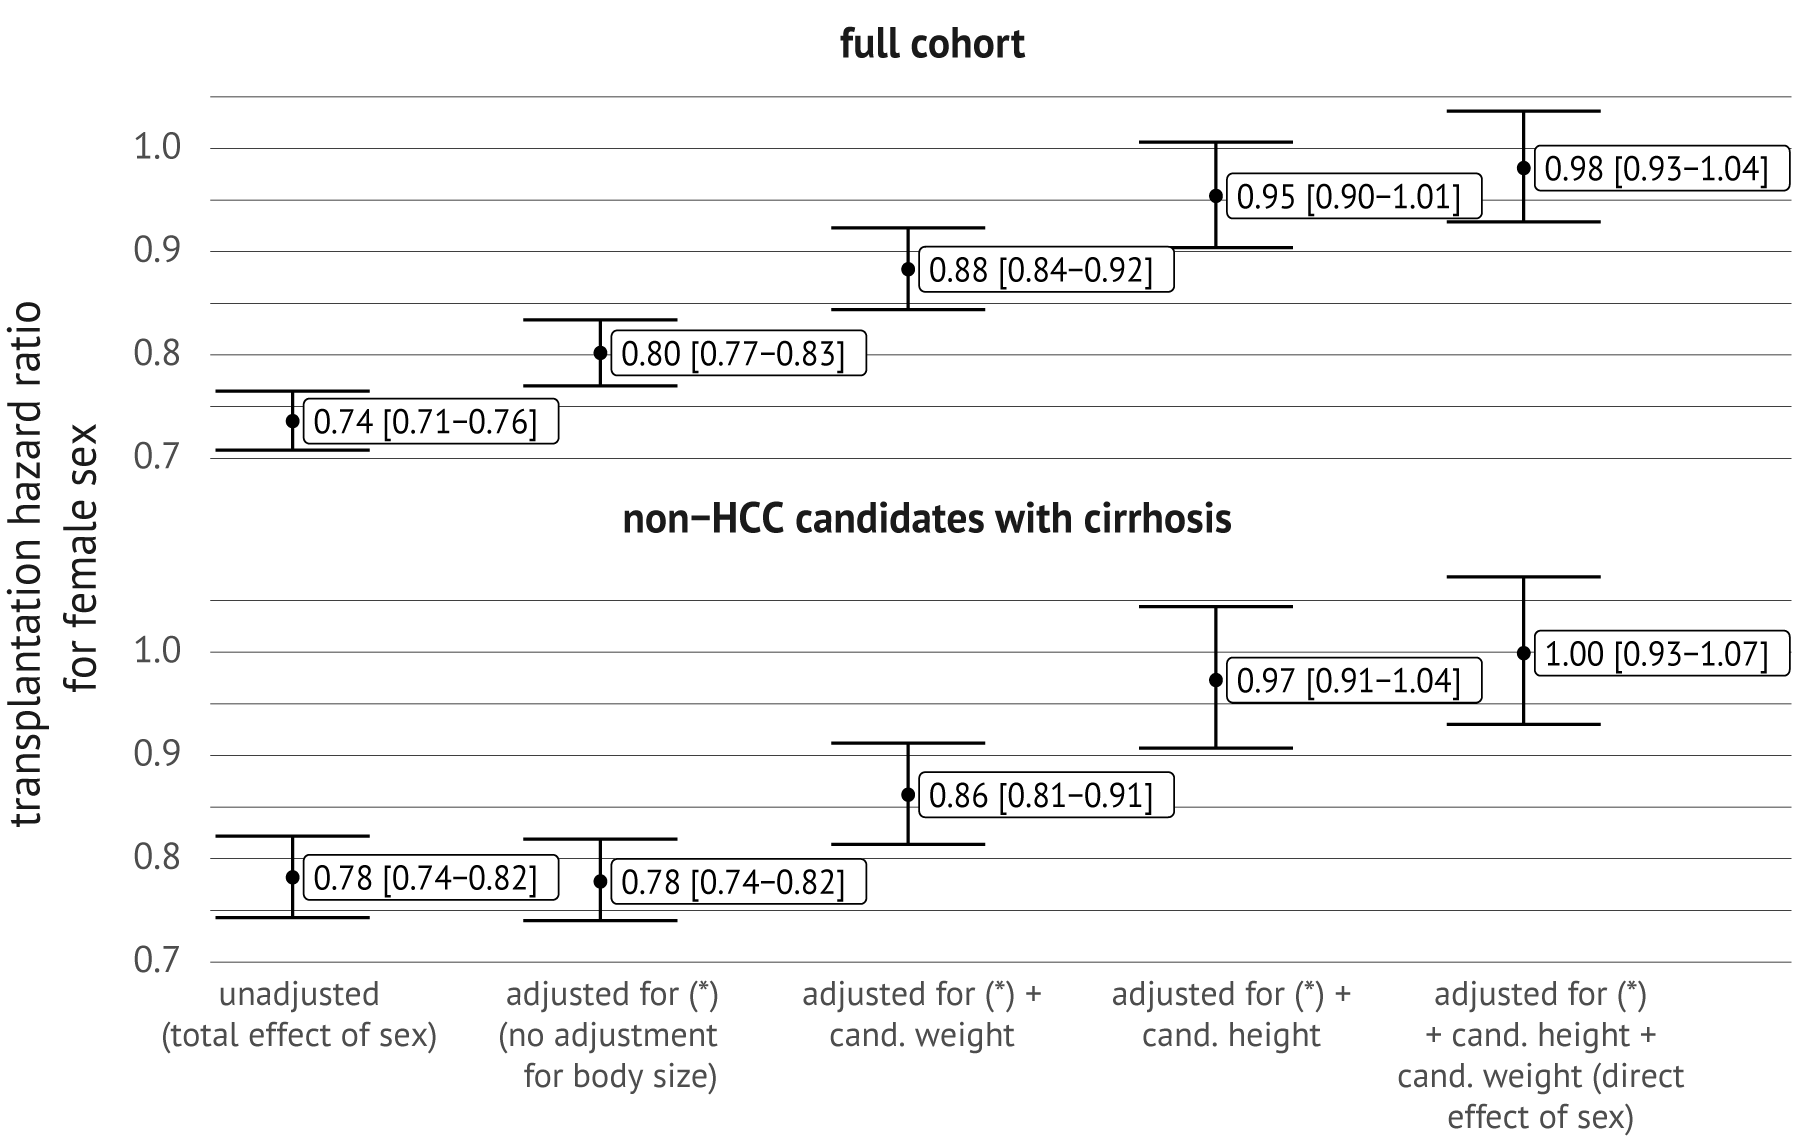
\includegraphics[width=1\linewidth]{figures/ch4/fig4_hr_txp} 

}

\caption{Estimates for the transplantation hazard ratios for female sex with 95\% confidence intervals, in the full cohort (top panel) and the subpopulation of non-HCC candidates with cirrhosis (bottom panel).}\label{fig:ch4fig4}
\end{figure}

\newpage

Table \ref{tab:ch4tab2} shows the results of sensitivity checks for this analysis.
The results are qualitatively similar when using transplantation through standard
allocation as the outcome (first row), and when estimating transplantation hazard
ratios in the countries without center offers (second row); in both cases,
the estimated hazard ratios are non-significant after
adjustment for mediators and confounders of the mediator-outcome relation.
Figure \ref{fig:ch4fig5} shows
estimated spline terms for the relation between the relative transplantation
rate and height or weight, separately for males and females. For both sexes,
a lower height or weight is associated with a reduced transplant rate.
Height-sex (p=0.48) and weight-sex (p=0.11) interactions are insignificant in
ANOVA tests.

\begin{table}[!h]
\centering
\caption{\label{tab:ch4tab2}Sensitivity checks for the transplantation hazard ratio of female sex. Numbers in square brackets are 95\% confidence intervals.}
\centering
\fontsize{10}{12}\selectfont
\begin{tabu} to \linewidth {>{\raggedright\arraybackslash}p{5.2cm}>{\raggedright}X>{\raggedright}X}
\toprule
sensitivity check & unadjusted effect of sex (total effect) & adjusted $^a$ + height and weight (direct effect of sex)\\
\midrule
\cellcolor{gray!10}{full cohort, non-rescue transplantation as the outcome} & \cellcolor{gray!10}{0.783 [0.749-0.819]} & \cellcolor{gray!10}{0.991 [0.930-1.055]}\\
\addlinespace[0.5em]
full cohort restricted to Germany and the Netherlands (no center offers) & 0.735 [0.700-0.772] & 0.962 [0.994-1.066]\\
\bottomrule
\end{tabu}
\parbox{\textwidth}{\footnotesize \smallskip $^a$Variables adjusted for are the following: match-MELD, disease group, biweekly dialysis, type of (non) standardized exception received, candidate blood group, candidate age, and time spent non-transplantable.}
\end{table}

\begin{figure}[ht]

{\centering 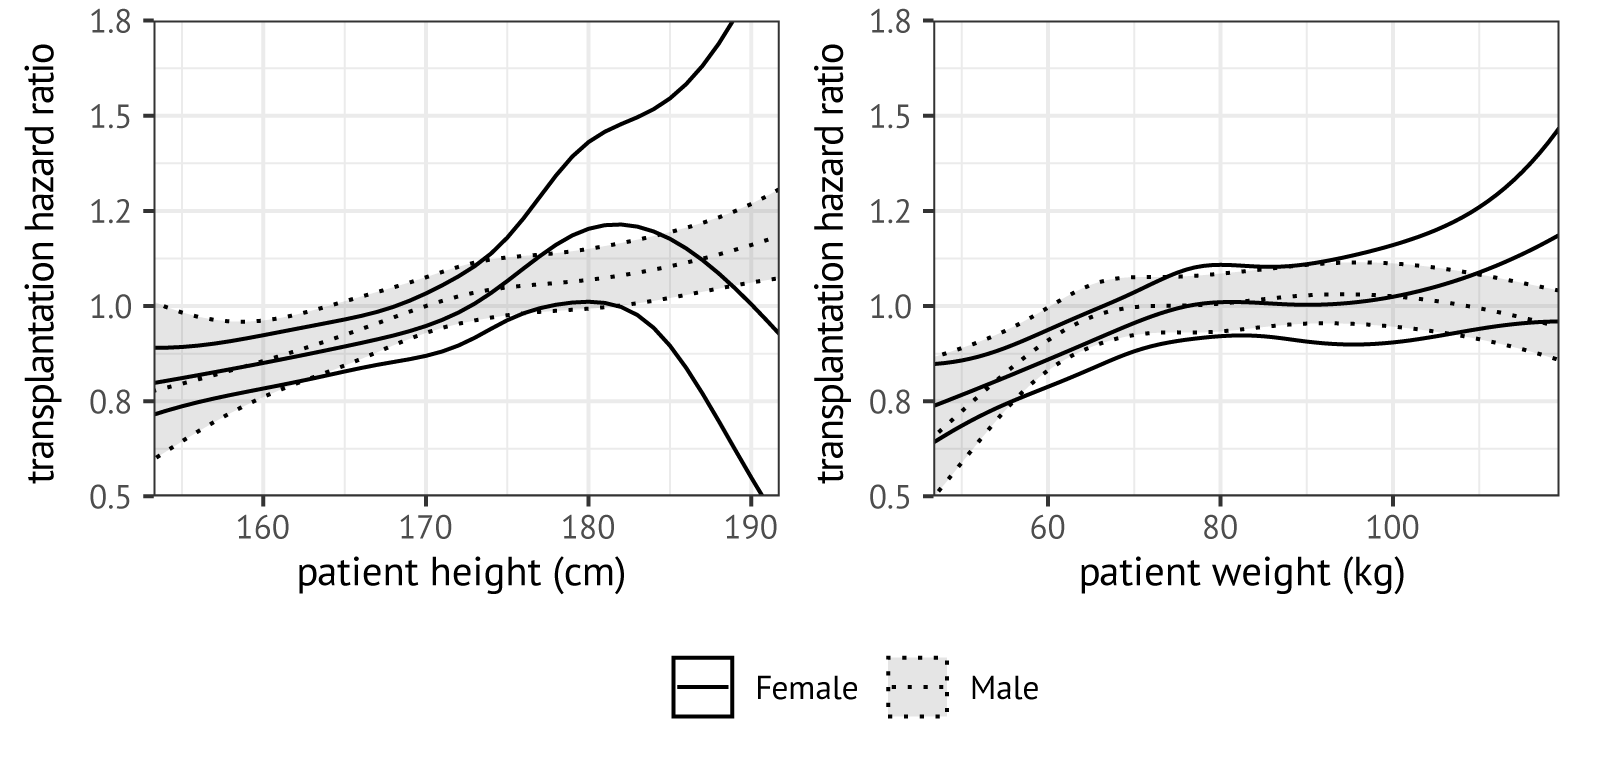
\includegraphics[width=1\linewidth]{figures/ch4/fig5_size_sex_interactions} 

}

\caption{Estimated relations between candidate height and the relative transplant rate, and candidate weight and the relative transplant rate, separately for males and females. These relations were estimated with cubic spline terms with 4 degrees of freedom.}\label{fig:ch4fig5}
\end{figure}

\subsection{Waiting list mortality analyses}\label{CHrsltsmediationmrt}

Figure \ref{fig:ch4fig6} shows estimates of the mortality hazard ratios for
female sex, adjusting for the lab-MELD score and confounders of the relation
between lab-MELD and the waiting list mortality rate. The waiting list mortality
hazard ratios include unity when adjusting for UNOS-MELD, both in the entire
cohort (HR = 1.03, 95\% CI: 0.88--1.20) and in non-HCC candidates with cirrhosis
(HR 0.94, 95\% CI: 0.80--1.11). Point estimates appear slightly increased for
MELD-Na and ReMELD-Na and decreased for MELD 3.0 (but confidence intervals include the null).

Table \ref{tab:ch4tab3} reports sensitivity checks for these results. With multiple imputation (MI), point estimates for MELD-Na, ReMELD-Na and MELD 3.0 are closer to the null. For MELD 3.0, the estimated hazard ratios become statistically significant, both in the full cohort (HR = 0.83, 95\% CI: 0.71--0.97) and in non-HCC candidates with cirrhosis (HR = 0.77, 95\% CI: 0.66--0.91). Results are similar when using waiting list death / removed unfit as a joint outcome (third row). Point estimates are slightly increased in candidates with high UNOS-MELD scores or
elevated creatinine, but remain statistically insignificant (except for ReMELD-Na in high-MELD candidates, 95\% CI: 1.02--1.59, fourth row). Results change little when estimated in Germany and the Netherlands, the Eurotransplant member countries without center offers (sixth row). Not correcting for dependent censoring with IPCW also appears to slightly increase point estimates.

\begin{figure}[ht]

{\centering 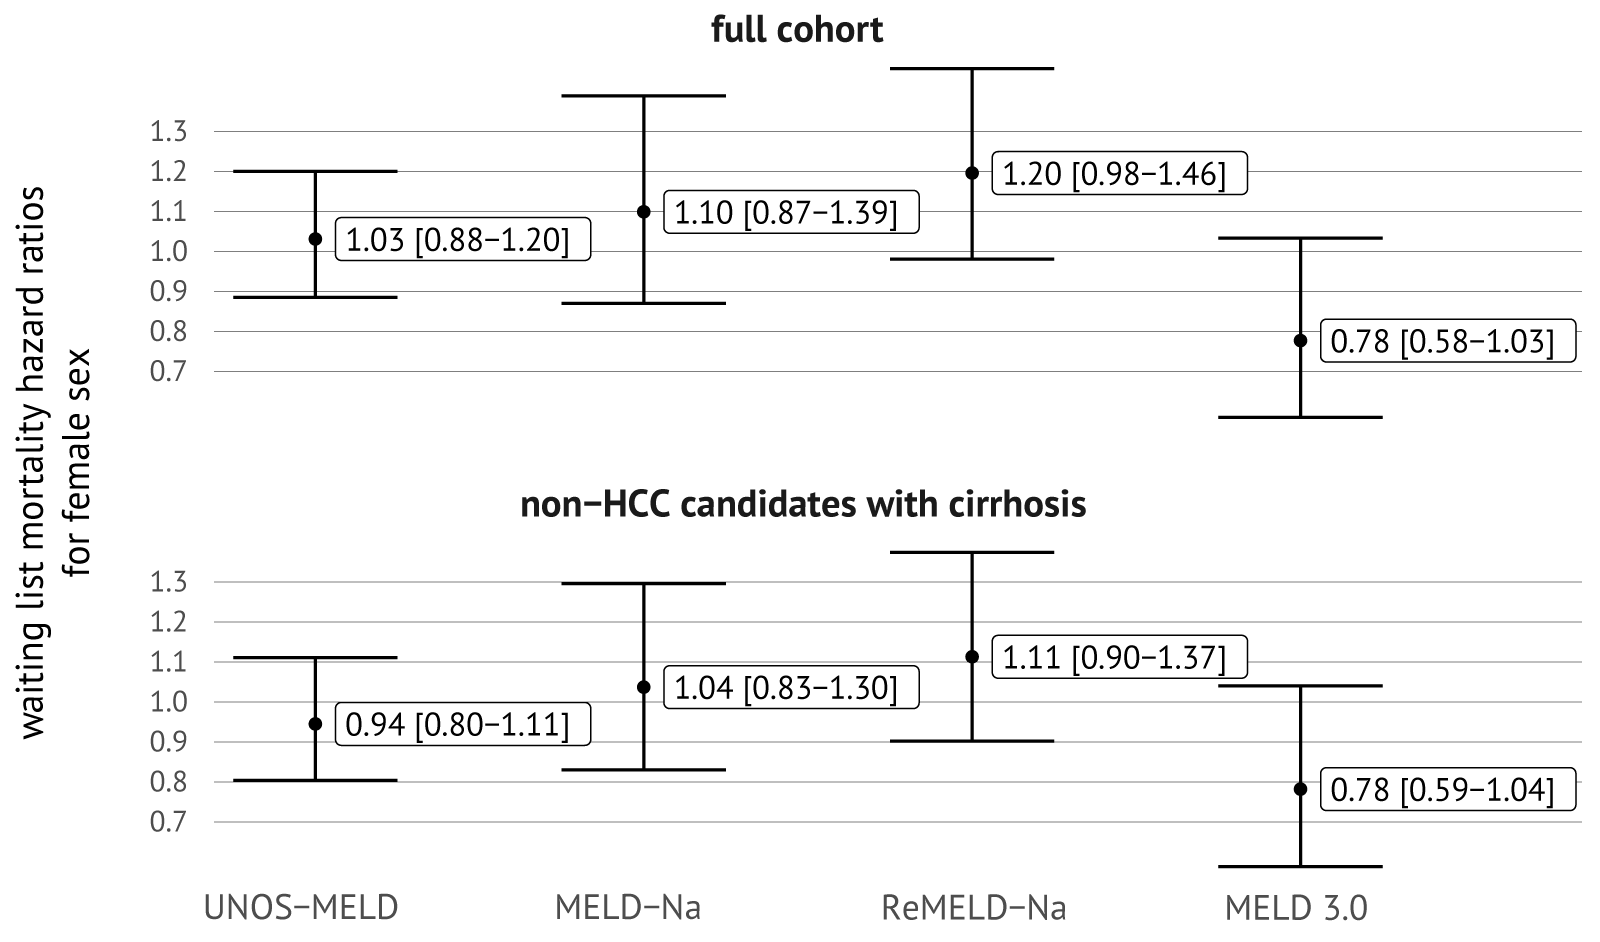
\includegraphics[width=1\linewidth]{figures/ch4/fig6_hr_mrt} 

}

\caption{Estimates for waiting list mortality hazard ratios for female sex with 95\% confidence intervals, with adjustment for a lab-MELD score (UNOS-MELD, MELD-Na, ReMELD-Na or MELD 3.0) and confounders of the relation between lab-MELD and waiting list mortality.}\label{fig:ch4fig6}
\end{figure}

\begingroup
\setlength{\aboverulesep}{0.2ex}
\setlength{\belowrulesep}{0.3ex}

\begin{table}
\centering
\caption{\label{tab:ch4tab3}Sensitivity checks for the waiting list mortality analyses. Shown are the hazard ratios and 95\% confidence intervals, estimated using IPCW with adjustment for MELD, and confounders of the relation between the MELD score and the transplant rate (candidate age, disease group, type exception and biweekly dialysis).}
\centering
\resizebox{\ifdim\width>\linewidth\linewidth\else\width\fi}{!}{
\fontsize{9}{11}\selectfont
\begin{tabu} to \linewidth {>{\raggedright\arraybackslash}p{3.7cm}>{\centering}X>{\centering}X>{\centering}X>{\centering}X}
\toprule
sensitivity check & UNOS-MELD & MELD-Na & ReMELD-Na & MELD 3.0\\
\midrule
\cellcolor[HTML]{F7F7F7}{\cellcolor{gray!10}{full cohort, with MI}} & \cellcolor[HTML]{F7F7F7}{\cellcolor{gray!10}{1.031 [0.885-1.200]}} & \cellcolor[HTML]{F7F7F7}{\cellcolor{gray!10}{1.038 [0.895-1.204]}} & \cellcolor[HTML]{F7F7F7}{\cellcolor{gray!10}{1.110 [0.958-1.285]}} & \cellcolor[HTML]{F7F7F7}{\cellcolor{gray!10}{0.831 [0.715-0.966]}}\\
\addlinespace[5pt]
non-HCC candidates with cirrhosis, with MI & 0.945 [0.804-1.111] & 0.956 [0.817-1.120] & 1.021 [0.872-1.196] & 0.773 [0.658-0.907]\\
\addlinespace[5pt]
\cellcolor[HTML]{F7F7F7}{\cellcolor{gray!10}{waitlist death or removed unfit as outcome}} & \cellcolor[HTML]{F7F7F7}{\cellcolor{gray!10}{1.002 [0.864-1.162]}} & \cellcolor[HTML]{F7F7F7}{\cellcolor{gray!10}{1.097 [0.874-1.376]}} & \cellcolor[HTML]{F7F7F7}{\cellcolor{gray!10}{1.190 [0.981-1.443]}} & \cellcolor[HTML]{F7F7F7}{\cellcolor{gray!10}{0.778 [0.589-1.028]}}\\
\addlinespace[5pt]
full cohort, MELD 18+ & 1.068 [0.908-1.257] & 1.180 [0.920-1.513] & 1.273 [1.022-1.587] & 0.866 [0.632-1.187]\\
\addlinespace[5pt]
\cellcolor[HTML]{F7F7F7}{\cellcolor{gray!10}{full cohort, creatinine $\geq$ 1.0 mg/dl}} & \cellcolor[HTML]{F7F7F7}{\cellcolor{gray!10}{1.118 [0.921-1.357]}} & \cellcolor[HTML]{F7F7F7}{\cellcolor{gray!10}{1.199 [0.889-1.615]}} & \cellcolor[HTML]{F7F7F7}{\cellcolor{gray!10}{1.249 [0.965-1.617]}} & \cellcolor[HTML]{F7F7F7}{\cellcolor{gray!10}{0.745 [0.509-1.089]}}\\
\addlinespace[5pt]
\addlinespace
recipient-driven countries & 1.018 [0.847-1.224] & 1.131 [0.832-1.539] & 1.225 [0.948-1.583] & 0.645 [0.427-0.974]\\
\addlinespace[5pt]
\cellcolor[HTML]{F7F7F7}{\cellcolor{gray!10}{full cohort, no IPCW}} & \cellcolor[HTML]{F7F7F7}{\cellcolor{gray!10}{1.097 [0.981-1.226]}} & \cellcolor[HTML]{F7F7F7}{\cellcolor{gray!10}{1.182 [0.994-1.404]}} & \cellcolor[HTML]{F7F7F7}{\cellcolor{gray!10}{1.226 [1.034-1.455]}} & \cellcolor[HTML]{F7F7F7}{\cellcolor{gray!10}{0.898 [0.700-1.151]}}\\
\addlinespace[5pt]
non-HCC candidates with cirrhosis, no IPCW & 1.034 [0.909-1.176] & 1.098 [0.908-1.328] & 1.135 [0.939-1.372] & 0.837 [0.639-1.096]\\
\addlinespace[5pt]
\bottomrule
\end{tabu}}
\parbox{\textwidth}{\footnotesize \smallskip \textbf{Abbreviations:} HCC, hepatocellular carcinoma; IPCW, inverse probability censoring weighting; MELD, model for end-stage liver disease; MELD-Na, model for end-stage liver disease sodium; MI, multiple imputation; ReMELD-Na, refitted MELD-Na for Eurotransplant; UNOS, United Network for Organ Sharing.}
\end{table}

\endgroup

\FloatBarrier

\subsection{Liver offer acceptance behavior}\label{liver-offer-acceptance-behavior}

To explore potential explanations for the reduced transplant rates among candidates
with a small stature, match lists generated between December 31, 2006
and December 31, 2019, were exported from the Eurotransplant database. Figure
\ref{fig:ch4sfigsize}
shows the distributions of weights and heights for these match lists,
separately for candidates and donors. The plot shows that candidates and donors have broadly similar height and weight distributions, with considerable overlap. Figure \ref{fig:ch4sfigoff} shows univariate
associations between graft offer acceptance and donor-candidate body size differences. The figure suggests
that size mismatch is indeed associated with declining
an organ offer. These associations are stronger if the
candidate weighs substantially lighter than the donor, or if the candidate is substantially
shorter.
\newpage

\begin{figure}[ht]

{\centering 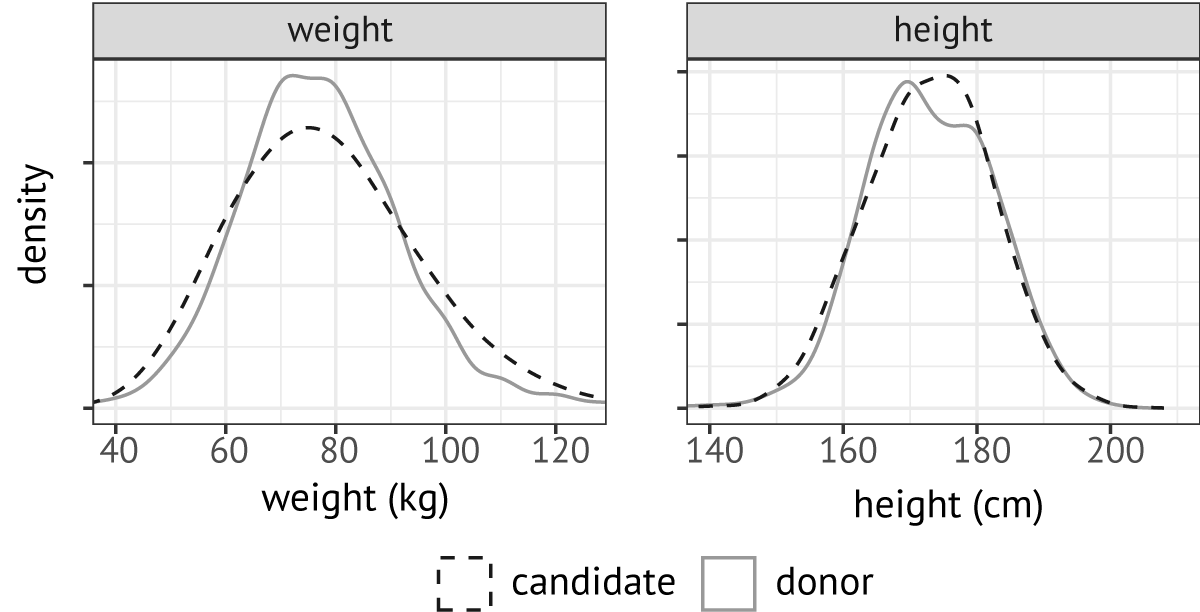
\includegraphics[width=0.75\linewidth]{figures/ch4/size_distr} 

}

\caption{Distributions of weights and heights for candidates and donors
  who appeared on Eurotransplant match lists between December 31, 2006 and December 31, 2019.}\label{fig:ch4sfigsize}
\end{figure}

\begin{figure}[ht]

{\centering 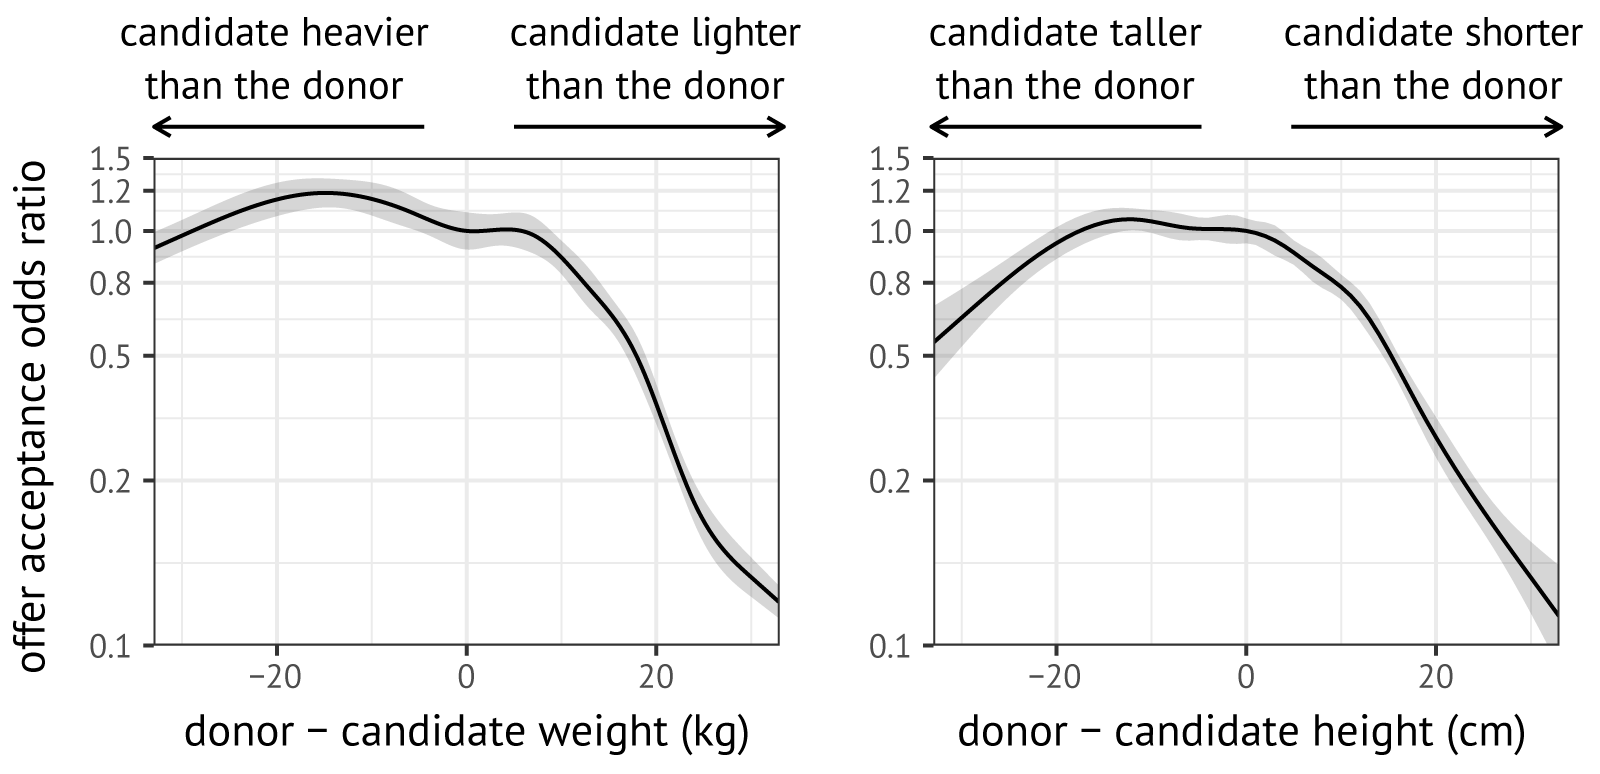
\includegraphics[width=0.9\linewidth]{figures/ch4/sfig_univariate} 

}

\caption{Univariate relations between the offer acceptance rate and the difference in donor and candidate body size, quantified through height or weight. These univariate relations were estimated with logistic models, using spline terms with 8 degrees of freedom.}\label{fig:ch4sfigoff}
\end{figure}

\FloatBarrier
\newpage

\section{Discussion}\label{discussion-1}

This chapter reports on sex disparity in liver waiting list outcomes in Eurotransplant.
Despite being listed at similar UNOS-MELD scores as males, relatively fewer females
are transplanted, and relatively more females die within 90 days of listing.
Similar results have been described in other geographic regions \citep{moylanDisparitiesLiverTransplantation2008, mathurSexBasedDisparitiesLiver2011, laiHeightContributesGender2010, lockeQuantifyingSexBasedDisparities2020a}.

We find that the transplant rates of females are approximately 25\%
lower than those of males in Eurotransplant, both in the full cohort
and among non-HCC candidates with cirrhosis.
This disparity disappears when adjusting for candidate height and weight, with
the estimated 95\% confidence intervals for the transplantation hazard ratio of
0.93--1.04 in the full cohort, and 0.93--1.07 in non-HCC candidates
with cirrhosis. Interactions of body
size with candidate sex are also insignificant, which suggests that small body
sizes are equally disadvantageous to males and females. We interpret these findings
as evidence for the size mismatch hypothesis: the smaller stature of female
candidates limits their chances of finding a suitable liver transplant, which results in sex disparity
in liver waiting list outcomes.

A potential explanation for the size mismatch hypothesis comes from the analysis
of the offer acceptance behavior of transplant centers: while weights and heights are similarly distributed in the donor
and patient populations, univariate analyses of offer acceptance
rates suggest that offers are more likely to be accepted for transplantation
when the donor has a similar or smaller body size than the patient. As a result,
there is high demand
for small organs, which disadvantages the small-statured patients who depend on
such offers for transplantation. Because these small-statured patients are predominantly
female, this also results in sex disparity.

Existing analyses from the United States have reported that females remain
disadvantaged after adjustment for age, height and weight, while our analyses
suggest that height and weight fully mediate the effect of sex on the transplantation
rate. This discrepancy could be explained by the fact that these existing
studies have adjusted for continuous variables either linearly
\citep{mathurSexBasedDisparitiesLiver2011, lockeQuantifyingSexBasedDisparities2020a} or with quantiles \citep{laiHeightContributesGender2010, nephewExceptionPointsBody2017},
instead of with non-linear spline transformations. We find that such
adjustment strategies bias hazard ratios downwards (results not shown).

Regarding waiting list mortality rates, we find that the hazard ratios for female
sex include the null when adjusting for UNOS-MELD and relevant confounders,
both in the full cohort and in non-HCC candidates with cirrhosis. We thus find
no evidence that females face higher waiting list mortality rates than males when
at the same UNOS-MELD score. In other words, we find no evidence for the
GFR hypothesis in our main analyses.
\newpage

Studies from the United States have reported higher waiting list
mortality rates for females when adjusting for MELD or its biomarkers. For example, Moylan
et al.~(2008) report a statistically significant hazard ratio of 1.09 for
female sex when adjusting for UNOS-MELD \citep{moylanDisparitiesLiverTransplantation2008},
Wood et al.~(2021) report that without-transplant survival is 0 to 5
percentage lower for females with MELD-Na \citep{woodCorrectingSexDisparity2021}, and
Kim et al.~(2021) find a hazard ratio of 1.23 in developing MELD 3.0 \citep{kimMELD3point0}.
Compared to these estimates, the point estimates we obtained in the main analyses
with adjustment for UNOS-MELD are low (1.03 in the full cohort, and 0.94 in non-HCC candidates with cirrhosis).

Our sensitivity checks lead to several potential explanations for this discrepancy.
Firstly, candidates in the United States are sicker than
candidates in Eurotransplant,
with median MELD-Na scores at transplantation of 27 in OPTN \citep{kwongOPTNSRTR20202022}
compared to 21 in Eurotransplant. We find that re-estimation of the mortality hazard
ratios in subgroups with higher MELD scores increases the estimated hazard ratio
for female sex slightly.
Secondly, 61\% of our cohort has low creatinine (\textless 1.0 mg/dl). For these
candidates, a systematically lower creatinine for females would not translate into
lower MELD scores, because MELD scores are calculated with a lower limit of 1.0
mg/dl for creatinine. When we re-estimate waiting list mortality hazard ratios
in the 39\% of candidates with elevated creatinine (≥1.0 mg/dl), the point
estimate increases to 1.12, which is more in line with existing literature
(although it remains statistically insignificant). We also find that not
correcting for dependent censoring by transplantation increases the point
estimates slightly.

A final difference is that our main results pertain to UNOS-MELD, whereas recent
studies adjust for scores which prioritize additionally on serum sodium (MELD-Na)
or serum sodium and serum albumin (MELD 3.0). With adjustment for
MELD-Na or ReMELD-Na instead of UNOS-MELD, our point estimates
of the waiting list mortality hazard ratio also increase to ±1.10 for MELD-Na
and ±1.20 for ReMELD-Na. They even become statistically significant in some
sensitivity checks for ReMELD-Na. These point estimates suggest
that the mortality rate of females is underestimated by 0.5 to 1 points on the MELD scale. When
adjusting for MELD 3.0 instead of UNOS-MELD, the point estimates for the mortality
hazard ratio are below 1. This suggests that the
1.33 extra points awarded to females in MELD 3.0 may overestimate the mortality
rates for females in Eurotransplant.

A clinical implication of our findings is that transplant centers should be aware of the
disadvantaged position of small-statured candidates when deciding whether to accept
a liver offer. Eurotransplant should also strive to rectify the sex disparity
that results from its current liver allocation algorithm. In the literature, the GFR hypothesis is frequently invoked
to motivate awarding points for female sex, either explicitly
\citep{kimMELD3point0} or indirectly by replacing creatinine in MELD by sex-specific
estimates of the GFR \citep{rodriguezPeralvarezDevelopmentValidationGenderEquity2023, myersGenderRenalFunction2011, asraniMELDGRAILNaGlomerularFiltration2020}.
By awarding points to females, such scores reduce sex disparity. However,
they do not target a smaller stature, which represents the root cause of sex disparity
according to our analysis.
\newpage

A more efficient way of addressing sex disparity could involve giving extra priority
to small-statured candidates, regardless of their sex. We point out that such an
allocation score cannot be developed solely based on a Cox proportional hazards
model which uses waiting list death as the outcome and which adjusts for MELD biomarkers
and candidate height. The reason for this is that body size only indirectly results in waiting list
deaths by limiting the transplant rate of small-statured candidates. This
indirect mechanism is not captured when modeling the waiting
list mortality with Cox PH models; rectifying sex disparity due to the size
mismatch hypothesis will require a different approach.

One such approach could be to develop allocation scores with simulation, as is done
by Wood et al. \citep{woodCorrectingSexDisparity2021}. A relevant proposal in this regard is a study by
Bernards et al., who assessed the effects of explicitly awarding points
to short candidates with Liver Simulation Allocation Model (LSAM) simulations
\citep{bernardsAwardingAdditionalMELD2022}. They report that awarding 1 extra MELD point
to the 8\% shortest waiting list candidates (\textless 156cm) is sufficient to result
in equalized outcomes across height groups in the United States. A similar
simulation study should be conducted for Eurotransplant, to assess how sex
disparity on the liver waiting list can be rectified.

Our study also has several limitations. Firstly, validity of the mediation analyses
depends on two unverifiable assumptions: no unmeasured confounding of mediator-outcome
relations, and the assumption that confounders of the body size-transplantation
rate act through candidate eligibility. Secondly, we rely on accuracy of
information in the Eurotransplant database. Thirdly, our quantifications of the direct
effect of sex on mortality are potentially underpowered when adjusting for
sodium-based MELD scores, as serum sodium is missing for most candidates in Eurotransplant registry
data. Fourthly, serum urea is not available in the Eurotransplant database such that
comparison to allocation scores which replace creatinine with estimated GFRs
was not possible.

In conclusion, this chapter has described sex disparities in liver waiting list
outcomes in Eurotransplant. In contrast to the existing literature, we lack
evidence that UNOS-MELD systematically underestimates pre-transplant
mortality rates in females. Our analysis instead suggests that transplantation
rates are lower in females because of their smaller stature. In addition to
externally validating MELD 3.0 and GEMA-Na, Eurotransplant should consider
prioritizing small-statured candidates to rectify sex disparity.

\chapter{The ELAS simulator}\label{CHelassimulator}

\chaptermark{The ELAS simulator}

\vfill

\begin{center}\rule{0.5\linewidth}{0.5pt}\end{center}

\noindent
An article based on this chapter has appeared in \emph{Operations Research, Data Analytics and Logistics}, de Ferrante, H.C., de Rosner-van Rosmalen M., Smeulders, B.M.L., Spieksma, F.C.R, Vogelaar, S., 2025, \href{https://doi.org/10.1016/j.ordal.2025.200476}{10.1016/j.ordal.2025.200476} \citep{deFerranteELASSimulator2025}

\newpage
\normalsize

\subsubsection*{Abstract}
In this chapter, we present the ELAS simulator. This discrete-event simulator
was built for the Eurotransplant Liver Allocation System (ELAS), which
is used by Eurotransplant to allocate the livers of deceased organ donors.
The simulator closely mimics ELAS and has been made publicly available
to (i) provide transparency regarding the models Eurotransplant uses to
evaluate liver allocation policies, and (ii) facilitate collaborations with
policymakers, scientists, and other stakeholders in evaluating
policy changes to ELAS. In this chapter, we describe the design and the modules
of the ELAS simulator. One of the included modules is the
obligation module, which is instrumental in ensuring that
international cooperation in liver allocation benefits all member
countries of Eurotransplant.

By default, the ELAS simulator simulates liver allocation according to
the actual Eurotransplant allocation rules. Stochastic processes, such
as graft offer acceptance behavior and listing for a repeat
transplantation, are approximated with statistical models that were
calibrated on data retrieved from the Eurotransplant database. We validate
the ELAS simulator by comparing simulated waiting list outcomes to
historically observed waiting list outcomes between January 1, 2016, and
December 31, 2019.

The ELAS simulator has a modular design, which gives end users maximal
control over the rules and assumptions under which Eurotransplant
liver allocation is simulated. This makes the simulator useful for
policy evaluation, as we illustrate with two clinically motivated
case studies. For these case studies, we collaborated with hepatologists and
transplantation surgeons from two liver advisory committees affiliated
with Eurotransplant.

\newpage
\normalsize

\section{Introduction}\label{introduction-2}

The Eurotransplant Liver and Intestine Advisory Committee (ELIAC) plays a key
role in developing liver allocation policies in Eurotransplant; ELIAC
monitors the Eurotransplant liver allocation system (ELAS) and makes proposals
to the Eurotransplant Board on how to improve liver allocation rules
according to the latest medical insights. Since the introduction of MELD-based liver
allocation in December 2006, ELIAC has brought forward several issues with ELAS; for
example, it has been reported that ELAS overprioritizes candidates who receive
exception points \citep{umgelterDisparitiesEurotransplantLiver2017a}, and that MELD
disadvantages candidates with small body sizes
\citep{Sneiders2023}.
Despite the identification of such issues, the current liver allocation
system has changed little since the initiation of MELD-based liver
allocation in Eurotransplant.

An important reason for the lack of policy change in ELAS is that Eurotransplant
has lacked tools that can help map the impact of allocation policy changes on liver
waiting list outcomes. There is a long history of using operations research and
discrete-event simulation for this purpose, with early work including the development of the UNOS
Liver Allocation Model (ULAM) for U.S. liver allocation \citep{Pritsker1995}.

In the United States, this work has culminated in the Simulation Allocation Models (SAMs)
\citep{ThompsonXSAM2004}, which is a family of discrete-event simulators
maintained by the Scientific Registry of Transplant Recipients (SRTR).
LSAM -- SRTR's tool for liver allocation \citep{ThompsonXSAM2004} --
is used routinely by the scientific community and
policymakers to study alternative liver allocation rules. For example,
LSAM has been used to study the impact of expanding MELD with extra
biomarkers \citep{kimHyponatremiaMortalityPatients2008a, kimMELD3point0},
the impact of alternative geographic sharing rules
\citep{freemanImprovingLiverAllocation2004, axelrodEconomicImplicationsBroader2011, gentryAddressingGeographicDisparities2013, goelLiverSimulatedAllocation2018, akshatHeterogeneousDonorCircles2024},
and the impact of policy changes that improve access to transplantation for
specific patient groups such as pediatric and female patients
\citep{peritoImpactIncreasedAllocation2019, heimbachDelayedHepatocellularCarcinoma2015, bernardsAwardingAdditionalMELD2022}. Other organ allocation organizations also
routinely note the use of simulators for evaluation of new liver allocation
policies, for example in France \citep{bayer2021removing} and the United
Kingdom \citep{Allen2024}.

Simulation can thus play a key role in moving Eurotransplant's liver
allocation system forward. This was recognized by Eurotransplant in the late
1990s, when computer simulations motivated a switch from ABO blood
group-identical liver allocation to the restricted ABO-compatible matching policies
that are still in use today \citep{demeesterWhichABOmatchingRule2002}. However, a simulation
model developed specifically for Eurotransplant has not been available.

Existing simulation models are also not applicable to Eurotransplant. Such models
typically simulate allocation for a single patient population, while Eurotransplant needs
to balance the interests of the populations from its eight member
countries. Moreover, existing models typically implement allocation
rules that are specific to the country for which the simulator was
designed. For example, allocation rules in LSAM emphasize the physical distance between the donor and transplantation
candidate, as geographical sharing in the United States is
primarily constrained by these physical distances. Conversely, in Eurotransplant,
geographical sharing is mostly impeded by country borders.
ELAS therefore gives priority to candidates who are located in the
same country as the donor, and implements a mechanism that
ensures that livers transplanted with priority across country borders are repaid
to the exporting country. These mechanisms have not been implemented for
existing simulation models, making these models a poor fit for Eurotransplant.

This has motivated us to develop a discrete-event simulator that is tailored to
ELAS. We refer to this simulator as the \emph{ELAS simulator}. Code for the
ELAS simulator is implemented in Python and made publicly available
together with synthetic data.\footnote{\url{http://github.com/hansdeferrante/Eurotransplant_ELAS_simulator}} By default, the ELAS simulator
simulates liver allocation according to Eurotransplant allocation rules.
The modular design of the simulator enables end users to use the
simulator for policy evaluation.

It is clear that the development of the ELAS simulation could not be
done, and was not done, in isolation. Multiple stakeholders were involved
in various phases of the project. In particular, members of the
Eurotransplant Liver and Intestine Advisory Committee (ELIAC), who are hepatologists and transplant surgeons who represent
Eurotransplant's member countries, have given feedback on numerous
occasions on the conceptual design of the simulator; also, at
Eurotransplant Annual Meetings, physicians and transplantation
coordinators have commented on various aspects of the simulator.

This chapter is structured as follows. In Section \ref{sec:elassystem}, we give a
description of Eurotransplant's liver allocation system (ELAS). In
Section \ref{sec:elasdesign} we
discuss the design of the ELAS simulator, and give an overview of the
general flow of the simulations. In Section
\ref{sec:elasmodules}, we
describe important modules of the ELAS simulator, each of which emulates
a key aspect of the liver allocation process. In Section
\ref{sec:elasvv},
we discuss verification and validation of the ELAS simulator. In Section
\ref{sec:elascasestudies}, we illustrate with two clinically
motivated case studies that the ELAS simulator is useful for policy
evaluation. We conclude and discuss in Section
\ref{sec:elasconclusion}.

\section{The Eurotransplant Liver Allocation System (ELAS)}\label{sec:elassystem}

We provide a simplified description of ELAS below. Comprehensive descriptions of ELAS
are available elsewhere
(see \citep{jochmansAdultLiverAllocation2017, ETLiverMan2025}). Fundamental to
ELAS is the laboratory MELD (lab-MELD) score, which quantifies a
candidate's 90-day waiting list mortality risk based on serum bilirubin,
serum creatinine, and the INR
\citep{kamathModelPredictSurvival2001}. However, candidate prioritization is not solely based on
lab-MELD scores, because certain patient groups would be underserved by
such an allocation.
\newpage
Specifically, ELAS also prioritizes candidates with:

\begin{itemize}
\item
  the High Urgency (HU) status,
\item
  the Approved Combined Organ (ACO) status that is given to
  candidates who require a combined transplantation of a liver with a
  heart, lung, pancreas, or intestine,
\item
  pediatric MELD (PED-MELD) scores that are assigned automatically to candidates
  of pediatric age,\footnote{younger than 18 in all countries since March 2025.} and
\item
  Standard and Non-Standard exception (SE / NSE) MELD scores that can be awarded
  to patients who require access to liver transplantation for other reasons than a high
  short-term mortality risk.
\end{itemize}

When a liver becomes available for allocation, Eurotransplant runs the liver
\emph{match algorithm} against a central database in which candidates for liver
transplantation are registered. This computer algorithm implements the
prioritization mechanisms of ELAS. Based on all the waiting candidates, this
algorithm returns a list of candidates eligible to receive the liver graft.
This match list is ordered based on donor and
candidate characteristics, and the order determines the sequence in
which candidates are offered the liver graft by Eurotransplant. An
actual Eurotransplant liver match list for an adult blood group A donor
reported from the Netherlands is shown in Table \ref{tab:ch5tab1}.

At the highest level, the Eurotransplant match list order is based on
\emph{match tiers}. Candidates in higher tiers have priority over
candidates in lower tiers. The first ELAS tier consists of candidates
with the High Urgency (HU) status. The second tier consists of
candidates with the Approved Combined Organ (ACO) status. Candidates
with HU or ACO status are given international priority in
Eurotransplant. A payback mechanism is used for grafts accepted internationally
in HU and ACO tiers. Specifically, international HU / ACO transplantations create an
\emph{obligation} for the receiving country to offer the next available liver
within the same blood group to the donor country until the obligation is
settled (see Section \ref{sec:elasobligations} for more information).
Candidates without an HU or ACO status are referred to as \emph{elective} candidates
in Eurotransplant. These elective candidates are ranked in the remaining tiers.

Whether candidates appear on the match list and the rank at which they appear
is jointly determined by patient \emph{eligibility} criteria (blood
groups), \emph{ranking} criteria (MELD, pediatric status, donor/recipient blood
group combination), and \emph{filtering} criteria (patients can indicate that they
do not want to be considered for certain donors with allocation
profiles). These patient eligibility criteria, ranking criteria, and
filtering criteria are multi-factorial and differ between the member countries of Eurotransplant.
\newpage

\begin{table}[h]
\caption{Example of a match list for an adult liver graft donated by a blood group A donor in the Netherlands. Under the restricted ABO blood group rules, candidates
  with blood group A and AB are eligible for this liver. At the moment of allocation, the Netherlands has an obligation to return a blood group A liver graft to Croatia, resulting in Croatian candidates being ranked higher than all Dutch candidates in the elective tiers. This specific liver graft was declined by all Croatian and Dutch candidates and finally transplanted into a Belgian recipient.}
\label{tab:ch5tab1}
\centering
\resizebox{1\ifdim\width>\linewidth\linewidth\else\width\fi}{!}{%

\begin{tabular}{lC{1.6cm}C{2.5cm}C{0.6cm}C{1cm}C{1cm}C{1cm}C{1cm}C{1cm}C{1.5cm}}
    \toprule
    \makecell{tier} & \makecell{offered to} & \makecell{candidate\\country} & \makecell{rank} & \makecell{match-\\MELD} & \makecell{lab-\\MELD} & \makecell{PED-\\MELD} & \makecell{(N)SE\\-MELD} & \makecell{cand.\\blood\\group} & \makecell{offer\\accepted?}\\
    \midrule
    HU & patient & Austria & 1 &  & 25 & 22 &  & AB & No\\
    \cmidrule{1-10}
    & \makecell{center\\(29 patients)} & Croatia & 2 &  &  &  &  &  & No\\
    \cmidrule{2-10}
    &  &  & 3 & 28 & 16 &  & 28 & A & No\\
    \cmidrule{4-10}
    &  &  & 4 & 22 & 22 &  &  & A & No\\
    \cmidrule{4-10}
    &  &  & 5 & 20 & 8 &  & 20 & A & No\\
    \cmidrule{4-10}
    &  &  & 6 & 20 & 20 &  &  & A & No\\
    \cmidrule{4-10}
    &  &  & 7 & 17 & 17 &  &  & A & No\\
    \cmidrule{4-10}
    &  &  & 8 & 17 & 17 &  &  & A & No\\
    \cmidrule{4-10}
    &  &  & 9 & 16 & 16 &  &  & A & No\\
    \cmidrule{4-10}
    &  &  & 10 & 15 & 15 &  &  & A & No\\
    \cmidrule{4-10}
    &  &  & 11 & 14 & 14 &  &  & A & No\\
    \cmidrule{4-10}
    &  &  & 12 & 14 & 14 &  &  & AB & No\\
    \cmidrule{4-10}
    &  &  & 13 & 14 & 14 &  &  & A & No\\
    \cmidrule{4-10}
    &  &  & 14 & 13 & 13 &  &  & A & No\\
    \cmidrule{4-10}
    &  &  & 15 & 13 & 13 &  &  & A & No\\
    \cmidrule{4-10}
    &  &  & 16 & 9 & 9 &  &  & A & No\\
    \cmidrule{4-10}
    &  &  & 17 & 9 & 9 &  &  & A & No\\
    \cmidrule{4-10}
    &  &  & 18 & 9 & 9 &  &  & A & No\\
    \cmidrule{4-10}
    &  &  & 19 & 8 & 8 &  &  & A & No\\
    \cmidrule{4-10}
    &  &  & 20 & 8 & 8 &  &  & A & No\\
    \cmidrule{4-10}
    &  & \multirow{-19}{*}{\raggedright\arraybackslash Netherlands} & 21 & 6 & 6 &  &  & A & No\\
    \cmidrule{3-10}
    \multirow{-21}{*}{\raggedright\arraybackslash elective} & \multirow{-20}{*}{\raggedright\arraybackslash patient} & Belgium & 22 & 35 & 35 &  &  & A & Yes\\
    \bottomrule
\end{tabular}
}
\end{table}

\FloatBarrier
\newpage

A rule common to all countries is that elective candidates listed in the same country
as the donor have priority over elective candidates listed in other countries. Other
factors that affect the ranking of candidates include the combination of the donor and
candidate blood groups, whether the donor and/or candidate are pediatric,
whether the adult is low-weight (\textless55 kg), as well as where the candidate is located
geographically relative to the donor (same center, same region, same country, or
different countries). The order of the match list in elective tiers is also affected by the existence of obligations.
For example, when the match list shown in Table \ref{tab:ch5tab1} was created, the Netherlands had an
obligation to offer a blood group A liver to Croatia. Consequently,
in the elective tier all Croatian candidates were ranked above the Dutch
candidates. The most important factor for ranking candidates in elective
tiers is the \emph{match}-MELD score (see Table
\ref{tab:ch5tab1}). This match-MELD score is the maximum of a candidate's lab-MELD
score and any received exception points (PED-MELD, SE-MELD, or NSE-MELD). We point
out that exceptional scores (SE-MELDs or NSE-MELDs) are valid only
for national allocation or when an offer is based on an obligation to pay back a liver.

Most offers in ELAS are \emph{recipient-driven}, which means that
Eurotransplant offers the liver graft to a named candidate
\citep{jochmansAdultLiverAllocation2017}. Under specific circumstances,
Eurotransplant makes a \emph{center offer} to candidates, which means that centers
are allowed to select any blood group compatible candidate from their waiting
list for transplantation. Offers to Croatia based on an obligation are an example of
center offers, which explains why a single offer to 29 Croatian patients appears
on the match list in Table \ref{tab:ch5tab1}. The position of center offers
on the match list is determined by the highest rank that is achieved by any
candidate listed in the center in elective tiers. We note that national regulations differ on
when offers are center-driven. These rules are described in the Eurotransplant
liver manual (see \citep{ETLiverMan2025}).

The order of the match list determines the sequence in which Eurotransplant contacts
centers in \emph{standard allocation}. In cases where the loss of a transplantable graft
is anticipated, Eurotransplant can deviate from this allocation order (see
\citep{jochmansAdultLiverAllocation2017, ETLiverMan2025}). For example, Eurotransplant
is allowed to start an \emph{extended allocation} procedure 2 hours before the planned
explantation procedure (1 hour in Germany). Centers in the vicinity of the donor
center are then contacted, and are given 30 minutes to propose up to two
candidates for transplantation. The proposed candidate with the highest rank
on the match list is then selected for transplantation. If extended allocation is unsuccessful, Eurotransplant can also offer
the graft to centers located further away from the donor center on a first-come, first-served basis
with \emph{competitive rescue allocation}. In
total, 20\% to 25\% of liver grafts are transplanted through \emph{non-standard} allocation
mechanisms \citep{jochmansAdultLiverAllocation2017}. Extended allocation accounts for the majority of these placements.
\vfill
\newpage

\section{The design of the ELAS simulator}\label{sec:elasdesign}

The ELAS simulator was designed to enable end users to assess the impact of changes
to the liver allocation rules on waiting list mortality rates and access to
transplantation. We follow existing literature
by using discrete-event simulation (DES) for this purpose \citep{shechterClinicallyBasedDiscreteEvent2005, Pritsker1995, ratcliffeSimulationModellingApproach2001, ThompsonXSAM2004}. With DES,
complex processes are analyzed by determining how system states are
affected by a sequence of discrete events. Within the ELAS simulator,
the system states are (i) the statuses of transplant candidates
(whether they remain alive, their last known MELD score, their accrued
waiting time, and other information used in allocation), and (ii)
obligations to return a graft. The discrete events which affect these
system states are (i) patient events, which directly modify the
candidate's state (e.g.~updates to the MELD score), and (ii) liver donation
events, which generally lead to the transplantation
of a candidate, and which may result in the creation or redemption of an
obligation to pay back a liver graft.

Which candidate is transplanted when a donor becomes available is affected by several stochastic processes.
One such process is the graft offer acceptance behavior of the transplant centers.
Such behavior plays a
key role in liver allocation because the transplant centers frequently
decline liver grafts they deem unsuitable for their candidates.\footnote{In fact, only 20\% of transplanted livers are accepted
  by the top-ranked candidate in Eurotransplant.} Another stochastic
process is that recipients of a
liver transplant can experience a early graft failure, and may be listed for a
repeat transplantation. To accurately simulate outcomes of the
Eurotransplant liver allocation process, the ELAS simulator also has to
mimic these stochastic processes.

For discussion of the design of the ELAS simulator, we find it helpful
to distinguish between

\begin{enumerate}
\def\labelenumi{\arabic{enumi}.}
\item
  the \emph{organ allocation environment}, with which we refer to the
  overall setting in which allocation policies operate. This
  environment is deterministically defined by the simulation settings
  and input streams. Of key importance are the simulation input streams, which
  are the datasets that define the donors which become available for
  transplantation, the candidates who appear on the liver waiting
  list, and the donor and patient events that drive ELAS simulations.
  These input streams also specify the nested structure of agents in
  the ELAS simulations: donors and patients are nested in hospitals and
  transplant centers, which are in turn nested in the
  Eurotransplant member countries. The organ allocation environment has
  to be specified in advance of any simulation. We discuss the
  requirements for input streams in Section
  \ref{sec:elasenvironment}. How simulations are
  initialized based on input streams is discussed in Section
  \ref{sec:elasinit}. How simulations proceed is
  illustrated in Section
  \ref{sec:elasoverview}, and
\item
  \emph{simulation modules}, which are implemented in Python code. These
  modules emulate key aspects of the liver allocation procedure. These
  processes include the generation of liver match lists according to
  ELAS' liver allocation rules, the simulation of graft offer acceptance
  behavior, ELAS' obligation system, and ELAS' exception point system.
  We discuss the implemented modules in Section
  \ref{sec:elasmodules}.
\end{enumerate}

With this overall design, the ELAS simulator is similar to LSAM, the simulator that
has been used extensively to study organ allocation in the United
States. We also point out several differences. Most importantly, the
ELAS simulator is developed specifically for Eurotransplant, and takes
into account the multi-national setting; we include international
sharing rules and allow for allocation rules to differ per country.
Other major differences include that (i) centers can decline
liver offers for all their candidates in ELAS simulations, (ii) the ELAS simulator can
approximate outcomes of non-standard allocation while LSAM always places
livers through standard allocation, (iii) organ offer acceptance models specific
to pediatric candidates are included, (iv) the splitting of liver grafts is
simulated, and (v) simulation of re-listing for repeat transplantation is
based on historical re-listing data.

\subsection{The organ allocation environment}\label{sec:elasenvironment}

To simulate liver allocation with the ELAS simulator, users must provide input
streams. These input streams consist of donor and patient information, which is
used by the ELAS simulator to construct the discrete events that drive the simulator.
Users of the ELAS simulator are free to base these input streams on actual
registry data, reordered registry data, synthetic data, or combinations
thereof. Ideally, the choice on which input stream is used is based on the end user's research question of interest. For example, end users
interested in evaluating the impact of small changes to allocation rules
may use historical data from the Eurotransplant registry for simulation,
while end users interested in evaluating the effect of an expansion to
the donor pool may need to extend the historical donor pool with synthetic
donor data.

The input stream for donors must specify all the administrative and medical information
that is required for liver allocation, for predicting the acceptance of liver offers,
or for predicting post-transplant survival. Such information includes the
donor reporting date, the donor hospital and donor reporting center, the donor weight
and height, the donor blood group, and the donor death cause. In the ELAS simulator,
this information is static and represents the state of the donor on the day they
were reported to Eurotransplant.

\newpage

Basic administrative and medical information necessary for allocation is also
required for the input streams for transplant candidates. Such information includes the candidate's center of listing,
the candidate's disease group, the candidate's age and weight, and the
candidate's blood group. To identify candidates listing for a repeat
transplantation, a candidate identifier must be specified. Next to
this static candidate information, dynamic information is required on
the evolution of candidate's medical condition while they await liver
transplantation. For this, the ELAS simulator requires an input stream
of candidate status updates. These status updates specify when and how a
candidate's state changes while they wait on the Eurotransplant waiting
list. Examples of such status updates are new biomarker measurements, the
reception of exception scores or upgrades thereof (NSE / SE / PED-MELD),
changes to the candidate's waiting list status (HU / ACO / NT status), and an
exit status for each candidate (waiting list removals or waiting list
deaths). Because candidates regularly modify their \emph{allocation
profiles}, profiles were also implemented as status updates. With these
allocation profiles, centers can indicate that a candidate does not want
to receive offers from certain liver donors. For example, many
candidates specify that they do not want to be offered grafts from
donors above a certain age threshold.

Discrete-event simulators for organ allocation require
complete knowledge on what would happen to a candidate if they would
remain on the waiting list until waiting list death or waiting list
removal. For candidates transplanted in reality, such information is
necessarily partly counterfactual; after all, transplantation prevents
us from observing what would have happened to the transplanted candidate
if they had remained on the waiting list. For other simulators, this
\emph{counterfactual status problem} was tackled by complementing the real
statuses of a transplanted candidate with statuses copied over from a
similar but not-yet-transplanted candidate
\citep{shechterClinicallyBasedDiscreteEvent2005, ThompsonXSAM2004}. We propose a
procedure that completes the status updates of transplanted candidates in this
way, and describe this procedure in detail in Appendix \ref{APPimputation}.

To summarize it briefly, the procedure first constructs a
\emph{risk set} for each transplanted
candidate. This is a set of candidates who
(i) remain on the waiting list, (ii) are similar to the candidate on a set of pre-specified characteristics, and (iii) face similar 90-day mortality risks
in the absence of transplantation. A complete status update trajectory can then be
constructed by (i) randomly sampling a candidate from the risk set, and
(ii) copying over the future status updates from the sampled candidate.
By running this procedure repeatedly, we construct for each candidate
multiple potential status update trajectories. This allows us to also
quantify the uncertainty in this status update completion
procedure in simulations.

\vfill

\subsection{Initialization of the ELAS simulator's system state}\label{sec:elasinit}

End users of the ELAS simulator must specify a simulation start and end
date, which jointly define the simulation time window. When the simulation
starts, the system state is initialized by loading from the input streams
all the donors who were reported during the simulation window, and all the
candidates who had an active waiting list status during the simulation window. For the
loaded candidates, all status updates are pre-processed until the
simulation start date. This ensures that the states of candidates at simulation start coincide with their actual status on the simulation start date, as
specified in candidate input streams.

A potential problem is formed by candidates who (i) have in reality received a
transplantation after the simulation start date and (ii) were listed for
repeat liver transplantation before the simulation end date, as these candidates
could simultaneously await a primary and repeat transplantation in simulation runs.
To prevent this, the ELAS simulator by default ignores re-listings
of such candidates from the candidate input stream. Instead, patient re-listing
is simulated by the post-transplant module. This module simulates the post-transplant survival,
and the potential re-listing of transplant recipients based on
candidate and donor characteristics (see Section \ref{sec:elasposttransplant}).

The initialization of the discrete-event simulation is finalized by
scheduling for each donor and transplant candidate a single event
in the Future Event Set (FES). For donors, events are scheduled at the
donor reporting date that is specified in the donor input stream. For each
candidate, a single patient event is scheduled at the time of the
candidate's first available status update after the simulation start
date. Subsequent updates are scheduled in the FES only after the
existing patient event has been handled.\footnote{This is necessitated by the
  fact that processing of a status update may result in automatic scheduling
  of a new update, see Section \ref{sec:elasexceptions}.}

\subsection{Overview of the simulation}\label{sec:elasoverview}

\begin{figure}[h]

{\centering 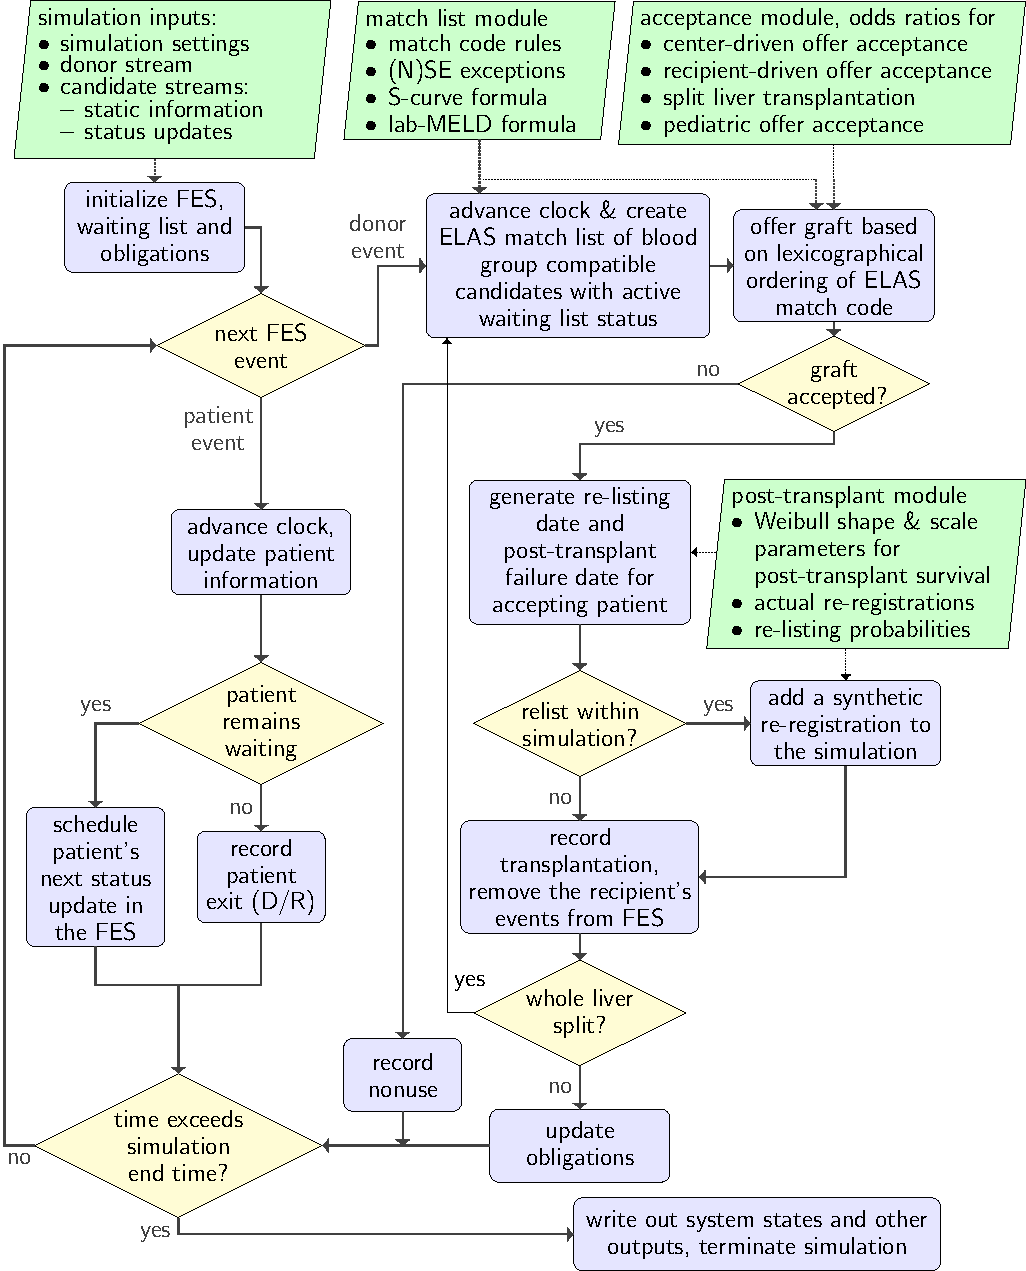
\includegraphics[width=0.9\linewidth]{figures/ch5//fig1-flowchart_liver_allocation} 

}

\caption{Event handling flowchart for the ELAS simulator. Inputs and parameters are represented using parallelograms. D, deceased on the waiting list; ELAS, Eurotransplant Liver Allocation System; FES, Future Event Set; MELD, Model for End-Stage Liver Disease; R, waiting list removal.}\label{fig:ch5fig1}
\end{figure}

Figure \ref{fig:ch5fig1} shows how patient and donor events from the
FES are processed in the ELAS simulator. In case of a patient event, the
corresponding candidate's status is updated according to their earliest
scheduled status update. In case a donor event is processed, a match list
is created. To appear
on this match list, candidates must have an active waiting list status
(T, HU, or ACO) and they must be compatible with the donor according to ELAS
blood group rules. The entities that appear on these match lists are offers
to patients and center offers (if applicable). These offers are ordered deterministically based on the allocation rules specified in the organ allocation
environment. By default, the actual ELAS allocation rules are followed,
which are summarized in Section \ref{sec:elasmatchlist}.

The ordered match list serves as an input to the graft offering module
(see Section \ref{sec:elasacceptance}). This module mimics the graft
offering process in Eurotransplant and returns the candidate who
accepts the liver offer, if any. We point out that it is not clear
based on the match list alone which candidate is transplanted with the liver.
One reason for this is that offers are regularly declined
by the transplant centers: in fact, over half of the transplanted liver
grafts in Eurotransplant were declined by 10 or more candidates before being accepted for transplantation. A second reason is that Eurotransplant can deviate
from the standard allocation procedure to prevent the loss of
transplantable organs (see Section \ref{sec:elassystem}). In simulating whether
a candidate accepts the offer, the module can simulate both standard and non-standard
allocation.

The ELAS simulator assumes that the candidate who accepts the liver
graft is transplanted, and removes any scheduled events for this
transplanted candidate from the Future Event Set. If a liver was allocated
across country borders in HU or ACO tiers, the obligation system module creates
an obligation for the importing country to return a liver graft in the future
(or settles an obligation for the exporting country, in case an existing obligation
exists). For livers exported based
on an obligation, obligations are also settled. The post-transplant module simulates
a time-until-liver-failure for each transplantation (see Section
\ref{sec:elasposttransplant}). In case the transplant recipient
is simulated to be listed for a repeat liver transplantation before
the candidate's simulated death date, the post-transplant module schedules a ``synthetic''
re-listing for the candidate (see Section \ref{sec:elassynthreg}).

The processing of patient and donor events continues until the
simulation end date is reached. At the end of the simulation, information
on transplantations is written to an output file. A list of discarded
grafts is also written to output files, as are the final states
of all candidates present in the simulation. These final states include
candidate exit statuses (waiting, waiting list death, transplanted, or
waiting list removal), as well as their last reported MELD scores. Such
information may be summarized to calculate the
statistics relevant for a specific research question. We chose to
write raw information to files rather than predefined summaries of
information to give end users maximum flexibility in reporting more
complicated statistics.

\section{Modules of the ELAS simulator}\label{sec:elasmodules}

This section describes the key modules of the ELAS simulator: the match list
module (Section \ref{sec:elasmatchlist}), the obligation system module (Section
\ref{sec:elasobligations}), the exception module (Section \ref{sec:elasexceptions}),
the graft offering module (Section \ref{sec:elasacceptance}), and the post-transplant module
(Section \ref{sec:elasposttxp}).

\FloatBarrier

\subsection{The match list module}\label{sec:elasmatchlist}

When a liver graft is to be allocated, the match list
module creates an ordered list of candidates who sequentially receive
offers until a candidate accepts the liver
graft. To appear on these match lists, candidates must (i) have an active
waiting list status (transplantable, HU, or ACO), and (ii) have a blood
group compatible with that of the donor, according to ELAS
allocation rules. By default, the match list module collapses offers to
candidates who are eligible for center offers into a single center offer object.
The rank of this center offer is set equal to the rank of the top-ranked candidate
eligible for that center offer. The match lists returned by the match list module
are thereby ordered lists of center-driven and patient-driven offers,
coinciding with the structure of match lists Eurotransplant actually uses
for allocation (see the example match list in Table \ref{tab:ch5tab1}).

The precise ordering returned by the match list module is based on the liver
allocation rules that must be pre-specified as part of organ
allocation environment. The rules made available with the ELAS simulator
are the ELAS allocation rules used between 2016 and 2024. end users of the
ELAS simulator can modify these allocation rules to study waiting list outcomes under
alternative allocation policies. Technically, the ranking of ELAS match objects (patient- or
center offers) is based on \emph{match codes}. These match codes
consist of several components. The values of these components are determined
by Eurotransplant allocation rules, donor and patient characteristics,
and the existence of obligations. Currently, these match codes consist of:

\begin{enumerate}
\def\labelenumi{\arabic{enumi}.}
\tightlist
\item
  \textbf{match tiers}, which are used to give international
  priority to patients with HU status or ACO status,
\item
  \textbf{match layers}, which differ per country and are used to give
  priority to certain patient groups (for example, to pediatric
  candidates, to blood group-identical candidates, to local
  candidates, or to candidates located in other countries based on
  obligations),
\item
  \textbf{match obligation ranks}, which are used as a tiebreaker in case
  the donor country has obligations to return livers to multiple
  countries,
\item
  \textbf{match-MELDs}, which are used to rank candidates in the elective
  tiers,
\item
  \textbf{match locality}, which is used to prioritize patients regionally
  in Germany in elective tiers,
\item
  \textbf{waiting time}, which is the number of days with a HU or ACO status
  in the HU and ACO tiers. In elective tiers, waiting time is defined as the
  number of days a candidate has had a match-MELD score at least as high
  as the current match-MELD score,
\item
  \textbf{the patient listing date}, which is used as a tiebreaker.
\end{enumerate}

The order of the match list is based on the lexicographical ordering of these
components.

\subsection{The obligation system module}\label{sec:elasobligations}

An important feature of Eurotransplant's obligation system is that
obligations within the same blood group are automatically \emph{linked}. For
example, if Croatia has an obligation to return a blood group A
liver to Belgium, and an obligation is created for Belgium to return a
blood group A liver to Germany, the two existing obligations are
replaced by a \emph{linked} obligation for Croatia to return a blood
group A liver to Germany.

The obligation module implemented for the ELAS simulator creates obligations
for grafts that are procured internationally in HU or ACO tiers, and automatically
replaces linkable obligations by a linked obligation. The module can also return
for a given blood group the outstanding obligations per country,
as well as the number of days these
obligations have existed. This information is required by the ELAS
simulator's match list module to determine match obligation ranks.

\subsection{The exception score module}\label{sec:elasexceptions}

Patient groups who are considered to be underserved by a purely
lab-MELD-based allocation can apply for standard (SE) or non-standard
(NSE) exceptions in ELAS. Candidates who receive such (N)SE and
PED-MELD scores are awarded predefined 90-day mortality equivalents,
which are specified in percentages. The exceptions, their eligibility criteria,
and their 90-day mortality equivalents vary by member country. For example,
in the Netherlands candidates with hepatocellular carcinoma are awarded a 10\%
mortality equivalent, while a 15\% mortality equivalent is awarded in Belgium.
Pediatric patients in Eurotransplant automatically receive PED-MELD scores based
on their age, which are also based on 90-day mortality equivalents.

For allocation, these mortality equivalents are translated to the MELD scale.
For example, a
10\% and 15\% mortality equivalent correspond to MELD scores of 20 and 22,
respectively \citep{ETLiverMan2025}. The awarded 90-day mortality equivalent
increases every 90 days\footnote{(N)SEs that require manual re-certification increase immediately after re-certification, which can occur 14 days before expiry (i.e., every 76--90 days). Simulations assume that these (N)SEs upgrade every 80 days in case no re-certification is known for the candidate. (N)SEs and PED-MELD with automatic re-certification increase every 90 days.} for most (N)SEs and PED-MELDs, according to
exception- and country-specific increments. Some exceptions are implemented
as ``bonus SEs''. These bonus SEs add a fixed percentage mortality equivalent to the
lab-MELD's 90-day mortality equivalent.\footnote{For example, a candidate with biliary
  sepsis in Germany with a MELD score of 21 would receive a 30 percent point
  bonus amount. Their lab-MELD score of 21 corresponds to a 90-day mortality
  equivalent of 26\%, giving them in total a 26\% + 30\% = 56\% mortality equivalent,
  which corresponds to a MELD score of 30.}

The exception score module implements this system, and is initialized
based on an external file. This file has to specify which exceptions
exist, and relevant exception attributes (the initial mortality
equivalent awarded, the 90-day increment, the maximal equivalent
awarded, the maximum age after which the exception no longer increases,
and whether the SE is a regular SE or a bonus SE). For the default organ
allocation environment, all (N)SEs and PED-MELDs existing in 2023 were
implemented. end users may modify the attributes of these exceptions to
simulate Eurotransplant liver allocation under alternative (N)SE / PED-MELD rules. Simulation settings
also have to include parameters for the formula used to translate 90-day
mortality equivalents to the MELD scale.\footnote{This transformation is based on a Cox
  proportional hazards model which uses MELD as the only predictor,
  and which uses a MELD score of 10 as the reference group. The curve used by Eurotransplant is given by: \[S_{90} = 0.98037 ^ {\exp\Big(0.17557(\texttt{UNOS-MELD} - 10)\Big)},\] where 0.98037 is the 90-day mortality equivalent for a MELD score of 10, and 0.17557 is the slope on MELD.}

By default, the ELAS simulator assumes that the candidate status input
stream also specifies when exceptions are upgraded or expire. In case no
future exception status is present in the candidate status queue for an
NSE / SE / PED-MELD, the ELAS simulator assumes that the candidate would
continue to re-certify their exception according to the
exception-specific re-certification schedule. This choice is motivated
by the fact that almost all candidates with exceptions re-certify them.

\subsection{The graft offering module}\label{sec:elasacceptance}

For a match list, the graft offering module returns the candidate who accepts the graft offer (if any), or indicates that all eligible candidates have rejected the offer. If the graft has been turned down for all eligible candidates, the simulator can either (a) force placement of the graft in
the candidate who was most likely to accept the graft offer, or (b)
record a discard.

The graft offering process is mimicked by (i) offering liver grafts to
patients/centers in order of their ranking on the match list, and (ii)
modeling organ offer acceptance as a Bernoulli process, with
acceptance probabilities predicted based on logistic models that using
donor and patient characteristics (as in the SAM software, see \citep{SRTR2019}).
The graft offering module also includes a logistic model to predict whether a
liver graft is split by the transplant center after acceptance.
Such split procedures allow centers to transplant two
candidates with one liver, and are typically performed to transplant one
pediatric and one adult patient.

There are several reasons why a candidate may not be offered a liver in
ELAS allocation despite being ranked high enough for an offer. These
reasons include that:

\begin{enumerate}
\def\labelenumi{\arabic{enumi}.}
\item
  Centers frequently decline the graft for all candidates who appear
  on the match list, even when making patient-driven offers (for
  example because of poor donor quality or capacity constraints). If centers decline for the entire center, the center will not be contacted again with an offer for the transplantation of a specific patient.
\item
  Offers are not made to candidates whose allocation profiles exclude
  them from being offered the liver graft (for
  example because the donor is too old).
\item
  Center offers are not directly offered by Eurotransplant to individual candidates.
  Instead, the transplant center chooses a candidate for transplantation.
\item
  Eurotransplant can deviate from the standard allocation procedure in
  case allocation time is limited. Offers
  to candidates not located in the vicinity of the graft are then
  bypassed.
\end{enumerate}

These reasons motivated us to

\begin{enumerate}
\def\labelenumi{\arabic{enumi}.}
\item
  Implement a two-stage patient-driven offer acceptance procedure. In
  the first stage, a center-level logistic model is used to predict
  based on donor characteristics alone whether the center is willing
  to accept the graft. Provided that the center is willing to accept
  the graft, a patient-level logistic model is used to predict graft
  offer acceptance based on patient and donor characteristics.
\item
  Skip offers to elective candidates whose allocation profiles indicate that they do not want to receive the liver graft.
\item
  Estimate logistic regressions separately for center- and
  patient-driven offers.
\item
  Approximate deviation from standard allocation (see \ref{sec:nonstandardalloc}).
\end{enumerate}

In the ELAS simulator, separate logistic models are used for four candidate groups:
(i) pediatric candidates
with HU / ACO statuses, (ii) elective pediatric patients, (iii) adult
candidates with HU / ACO statuses, and (iv) elective adult candidates.
This stratification is motivated by findings in the existing
literature that a single acceptance model poorly captures offer
acceptance behavior for specific patient groups. For example, Wood et al.
\citep{WoodPEDLSAM2021} note poor prediction for pediatric patients in LSAM.

To enable end users to change how graft offer acceptance decisions are
made, the odds ratios necessary for calculating the graft offer acceptance
probabilities are kept in csv files external to the program. Default
odds ratios supplied with the ELAS simulator were estimated based on
offers of whole liver grafts procured between January 1, 2012 and December 31, 2019.
When estimating these odds ratios, we ignored offers that were incompatible with
the allocation profiles of candidates and offers that were accepted
in non-standard allocation. To account for correlations in organ
acceptance behavior, odds ratios were estimated with mixed effect models. In these
models, we included random effects for donor heterogeneity (as in
\citep{agarwalEquilibriumAllocationsAlternative2021}), patient heterogeneity,
and center heterogeneity.

\subsubsection{Simulation of non-standard allocation}\label{sec:nonstandardalloc}

Approximately 25\% of livers are placed through non-standard allocation in
Eurotransplant. Without approximating such deviation from non-standard allocation,
the ELAS simulator would place too many grafts nationally in Belgium and Germany,
as both countries have implemented rules to prioritize local offers in
non-standard allocation. This motivated us to approximate deviation from standard allocation in the
graft offering module.

To address this, we approximate the initiation of non-standard allocation by

\begin{enumerate}
\def\labelenumi{\arabic{enumi}.}
\item
  simulating the maximum number of offers until non-standard allocation
  is initiated with a Cox proportional hazards model. This Cox model models
  the probability that non-standard allocation is triggered based on
  donor characteristics (malignancy, death cause, drug abuse, marginal
  donor criteria, virology), using the number of offers made as the timescale.
  The Cox model was stratified by donor country
  and blood group. The baseline hazards
  for this Cox proportional hazards model are shown in Figure \ref{fig:ch5sfig5}.
\item
  offering the graft in the order of the match list, while maintaining a
  count of the number of offers made,
\item
  if the maximum number of offers is reached

  \begin{itemize}
  \item
    stop offering the graft to candidates whose allocation
    profiles exclude rescue donors,
  \item
    give priority to regional candidates in Germany and
    to local candidates in Belgium.
  \end{itemize}
\end{enumerate}

In counting the number of offers made, a center-level rejection is
counted as a single offer, and a candidate-level rejection is counted
only if (a) the graft was compatible with the candidates allocation
profile and (b) the graft was previously rejected by fewer than five
candidate from the same center.

\begin{figure}[ht]

{\centering 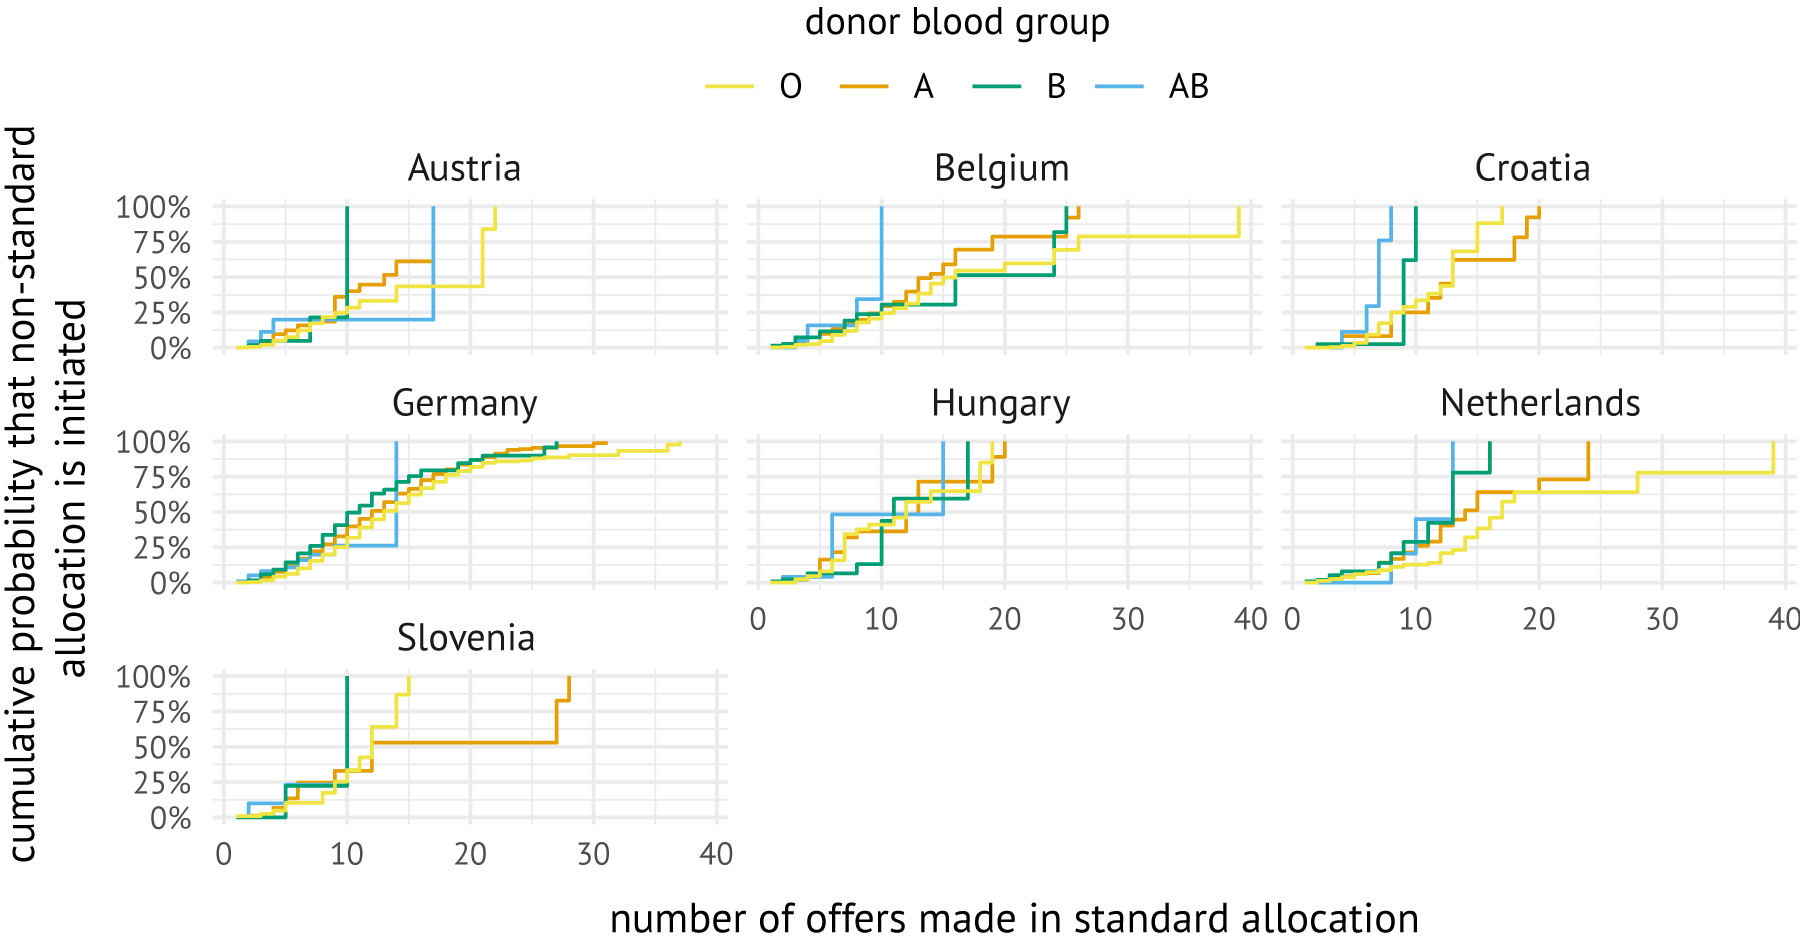
\includegraphics[width=1\linewidth]{figures/ch5//sfig5-init_rescue} 

}

\caption{The relation between the number of offers made in standard allocation and the probability that non-standard allocation is initiated. The country- and blood group-specific survival curves were generated by predicting the number of offers for an average patient.}\label{fig:ch5sfig5}
\end{figure}

\FloatBarrier

We note that this implementation is a heavily simplified representation of
non-standard allocation in Eurotransplant. Because candidates are still
prioritized based on the match list order, this implementation is closer to
extended allocation than to rescue allocation (which operates on a first-come, first-served basis). Implementing competitive rescue allocation
was not pursued because (i) it is not clear from donor information alone when
competitive rescue allocation is initiated, (ii) there are three types of
competitive rescue allocation in Eurotransplant, and (iii) not all centers are willing to accept grafts via competitive rescue allocation \citep{ETLiverMan2025}.

\subsection{The post-transplant module}\label{sec:elasposttxp}

Over 10\% of liver waiting list registrations in Eurotransplant concern
candidates who are listed for a repeat liver transplantation. To
accurately simulate such re-listings, a post-transplant module was
implemented for the ELAS simulator. Upon transplantation, this
module simulates a time-to-failure \(t\), defined as the time at which the
candidate would die in absence of re-transplantation. \(T\) is modeled using
a Weibull distribution, with parameters for recipient and donor characteristics.
The module also simulates a time-to-relisting \(r\), at which the candidate
enlists for a repeat transplantation.
Finally, if a candidate is simulated to list for a repeat transplantation,
the post-transplant module adds a listing for the repeat transplantation of
that candidate to the waiting list.
\newpage
The parameters needed to simulate the post-transplant survival of liver transplantation
recipients were estimated on Eurotransplant liver transplantations between January 1, 2012
and December 31, 2019. Since we expected post-transplant survival and re-listing to
be different for elective candidates and those with the HU or ACO status, we estimated the
parameters separately for these groups.

\subsubsection{Simulating time-to-failure for transplant recipients}\label{sec:elassimposttxp}

A Weibull model is used to simulate a time-to-event until patient death or
liver transplantation, separately for HU/ACO and elective candidates.
The used Weibull distribution is parametrized with a shape
parameter \(k\) and scale parameter
\(\lambda = \beta^{\T}x\) where \(x\) are relevant patient and
donor characteristics. The survival function for the Weibull distribution is given by:
\[S(t|x) = \exp\Bigg(-\Big(\frac{t}{\beta^{\T}x}\Big)^k\Bigg).\]

After
obtaining estimates for \(\beta\) and \(k\) based on historical data using Weibull
regression, a time-to-event \(t_i\) for a patient-donor pair \(i\) can be simulated by inverse transform sampling from this distribution. Specifically, we can draw a random
number \(u \sim \texttt{unif}(0,1)\) and simulate a patient's
time-to-event as
\[t_i = \hat{\mathbf{\beta}}^{\T} \mathbf{x_i} \Big(-\ln(u)^{\frac{1}{k}}\Big).\]

By default, post-transplant survival of elective candidates is simulated based
on a broad set of patient attributes (MELD biomarkers, patient age, country, sex, exception
scores, BMI), donor attributes (year reported, donor age, split, DCD or DBD, death cause,
malignancy, tumor history), and match attributes (candidate-donor weight difference, travel time,
blood group compatibility, match geography). Paucity of data on HU and ACO transplantations
motivated us to adjust for fewer variables in the non-elective model (weight difference,
donor death cause, donor age, patient age, lab-MELD score, match geography, and an
indicator for transplant history). Country-specific shape parameters are used to simulate \(t\) for elective
candidates, while a single shape parameter is used to simulate it for candidates
with the HU or ACO status.
\newpage

\subsubsection{\texorpdfstring{Simulating a time-to-relisting \(r\) for transplant recipients}{Simulating a time-to-relisting r for transplant recipients}}\label{sec:elassrelisting}

The simulation of a candidate's time-to-relisting is complicated by the fact that
a patient's time-to-relisting \(r_i\) necessarily has to occur before their
time-to-failure \(t_i\). To simulate re-listing times in the ELAS simulator, we
estimated the probability of re-listing using the Kaplan-Meier estimator, with the
time elapsed relative to the event time \(t_i\) as the timescale. A
re-listing time can then be simulated by inverse transform sampling from the
Kaplan-Meier curve, i.e., (i)
sample a random \(u \sim \text{unif}(0,1)\), (ii) choose the first \(s\) such that \(\mathbb{P}[R/T > s] \geq u\), and (iii)
calculate the time-to-relisting as \(s \cdot t\).

In case no such \(t\) exists, the patient will die without being listed for repeat
transplantation. The estimated empirical distribution of \(R\) relative to \(T\) is
shown in Figure \ref{fig:ch5sfig6}, stratified by discretized \(T\). The figure
shows that the fraction of patients who have died without having listed for
repeat transplantation depends strongly on their time-to-failure \(T\). For example, almost 70\% of
candidates who experience an event within one week after transplantation are
listed for a repeat liver transplantation, while only 20\% of candidates
who experience an event more than five years after initial transplantation are
listed for repeat transplantation.

\begin{figure}[ht]

{\centering 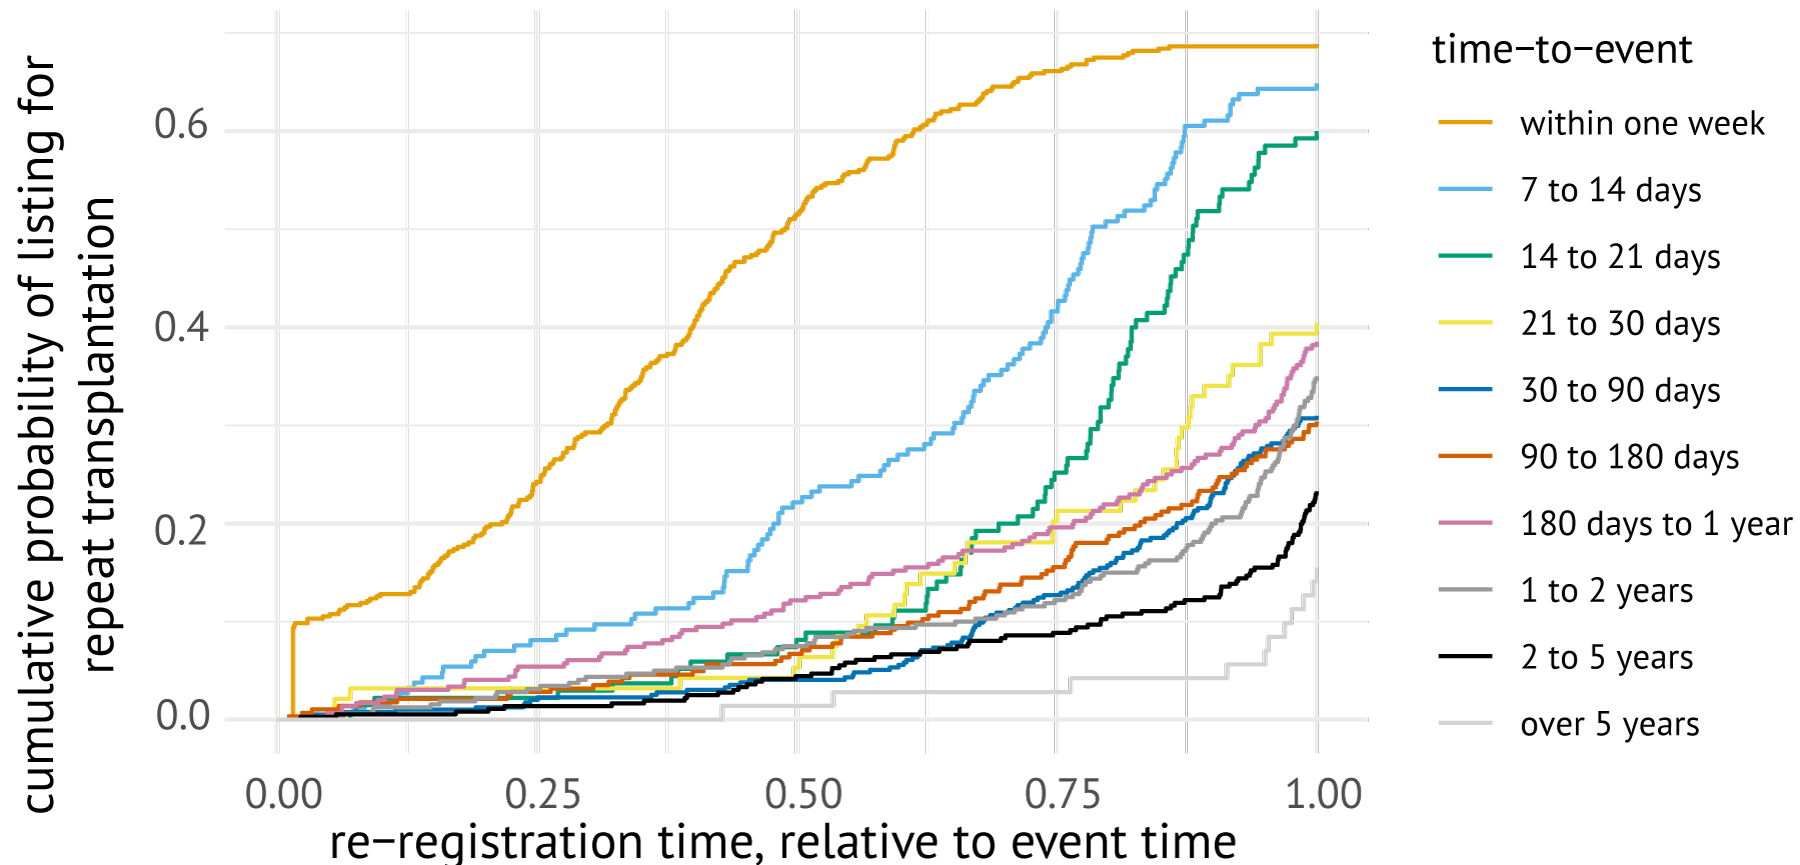
\includegraphics[width=1\linewidth]{figures/ch5//sfig6} 

}

\caption{Cumulative incidence curves showing the probability of listing for repeat transplantation, stratified by time-to-event categories. These curves were estimated with the Kaplan-Meier estimator based on candidates transplanted between January 1, 2012 and December 31, 2019.}\label{fig:ch5sfig6}
\end{figure}

\newpage

\subsubsection{Construction of synthetic re-registrations}\label{sec:elassynthreg}

If a candidate is re-activated on the waiting list before
the simulation end date, i.e., \(r\) \textless{} \(t\), the post-transplant module adds a \emph{synthetic} repeat
listing to the waiting list. This synthetic listing is
generated by combining the fixed patient characteristics of the transplant recipient
with the dynamic status updates of a candidate who was actually
re-listed for transplantation. This re-listing is chosen such that the candidates (a) have
similar time-to-failure \(t\) and similar time-to-relisting \(r\), and (b) match on
a pre-specified set of characteristics.

By default, the post-transplant module finds a matching re-registration
\(k\) by:

\begin{enumerate}
\def\labelenumi{\arabic{enumi}.}
\item
  Considering re-listings where candidates match in terms of whether
  they were re-listed within 14 days\footnote{Patients that are re-listed for liver
    transplantation within 14 days of transplantation can be eligible for an HU
    status under the current allocation rules \citep{ETLiverMan2025}.} after transplantation,
  were listed in the same country, are similarly aged (\textless20 years difference),
  and have a similar time-to-relisting and time-to-event (both \textless1 year difference),
\item
  Selecting from these potential re-listings the m=5 listings for repeat transplantation with the closest Mahalanobis
  distance between (\(r_i\), \(t_i\)) and (\(r_k\), \(t_k\)), and
\item
  Sampling one re-listing at random from these \(m\) re-listings.
\end{enumerate}

A synthetic re-listing is then constructed by combining the patient
attributes from transplant recipient \(i\) with status updates from patient \(k\).
The post-transplant module does not copy profile status updates from \(k\) to \(i\), as these allocation profiles are considered patient-specific. Exception scores from \(k\) are copied only if both patients were listed in the same country, since certain (N)SEs are associated with listing for repeat transplantation (e.g., hepatic artery thrombosis).

\section{Verification and validation}\label{sec:elasvv}

The previous section described the design of the ELAS simulator and
its modules. In
this section, we describe our efforts to ensure that the ELAS simulator
adequately represents ELAS. For this, we distinguish between model
\emph{verification}, which refers to efforts taken to identify coding errors in the
software, and model \emph{validation}, which refers to efforts taken to assess whether
simulated outcomes closely approximate actual outcomes of Eurotransplant
liver allocation. For a general discussion of model verification and model
validation, we refer to Carson \citep{carsonVerificationValidationConsultants1989}.

\subsection{Verification}\label{sec:elasverification}

To implement liver allocation rules in the ELAS simulator, we have used
the 2016 functional specifications for ELAS. To verify the correctness
of our implementation of ELAS allocation rules, we exported ELAS match
lists for 500 randomly selected donors who were reported between
January 1, 2016 and December 31, 2019. We constructed unit tests to verify that
the ELAS simulator correctly generated the match codes for these lists based
on the reported donor and candidate information. We also constructed unit tests to
ascertain that the simulator returned candidates in exactly the same order as the exported match lists.

To ensure the correctness of the exception module, we exported (N)SE
exception score definitions directly from the Eurotransplant database.
For the obligation system module, we used the functional specifications of
the ELAS obligation system to guide our implementation. These functional
specifications contain examples of how obligations have to be linked, including how to date the obligations that arise from multiple linkable
obligations. We implemented these examples as unit tests for the ELAS
simulator.

\subsection{Validation}\label{sec:elasvalidation}

Discrete-event simulators for organ allocation are typically validated
by comparing simulated statistics over a set time window to the actual
statistics from the same time period
\citep{ThompsonXSAM2004, shechterClinicallyBasedDiscreteEvent2005}. Properties commonly
validated are the number of transplantations and waiting list deaths,
typically also stratified by patient groups. We follow this practice to
validate the ELAS simulator.

We do not use traditional hypothesis testing (or confidence intervals) to compare
simulated and actual statistics, as
\emph{``traditional hypothesis testing is not appropriate for measuring model validity
because the null hypothesis that the true system and model are identical is almost
always false''}
\citep{shechterClinicallyBasedDiscreteEvent2005}. In fact, any difference
between actually observed outcomes and simulations can be made
statistically significant by increasing the number of simulation runs.
Instead, we give insight into the variability of ELAS simulator outputs
by reporting 95\% interquantile ranges (95\% IQRs) for simulation runs.
These interquantile ranges are obtained by simulating liver allocation
200 times, and reporting the 2.5th and 97.5th percentiles for simulated
outcomes of interest. When the real
summary statistic for an outcome of interest falls within the 95\%
interquantile range, we say that the ELAS simulator is
\emph{``well-calibrated''} for this outcome.

For input-output validation, we simulate Eurotransplant liver
allocation 200 times between January 1, 2016, and December 31, 2019.
The donor input stream consists of all 6,417 donors that were reported in this simulation window whose
livers were transplanted after allocation through ELAS. Characteristics of these
donors are shown in Table \ref{tab:ch5tab1donors}. The candidate input stream
consists of all patients who had an active waiting list status in the simulation
period. In total, these are n=7,137 patients who were activated on the waiting list between
January 1, 2016, and December 31, 2019 (see Table \ref{tab:ch5tab1patlisted}),
and n=1,831 patients waiting on January 1, 2016 (see Table \ref{tab:ch5tab1patincumbents}).

\begin{table}[!h]
\centering
\caption{\label{tab:ch5tab1donors}Characteristics of the donors used for simulation.}
\centering
\resizebox{\ifdim\width>\linewidth\linewidth\else\width\fi}{!}{
\fontsize{10}{12}\selectfont
\begin{tabular}[t]{>{\centering\arraybackslash}p{6em}lccccccc}
\toprule
variable & level & \makecell{Austria\\(n=610)} & \makecell{Belgium\\(n=1160)} & \makecell{Croatia\\(n=514)} & \makecell{Germany\\(n=2927)} & \makecell{Hungary\\(n=406)} & \makecell{Netherlands\\(n=672)} & \makecell{Slovenia\\(n=128)}\\
\midrule
 & female & 292 (47.9\%) & 496 (42.8\%) & 241 (46.9\%) & 1375 (47.0\%) & 180 (44.3\%) & 327 (48.7\%) & 53 (41.4\%)\\
\cmidrule{2-9}
\multirow{-2}{6em}[1\dimexpr\aboverulesep+\belowrulesep+\cmidrulewidth]{\centering\arraybackslash sex} & male & 318 (52.1\%) & 664 (57.2\%) & 273 (53.1\%) & 1552 (53.0\%) & 226 (55.7\%) & 345 (51.3\%) & 75 (58.6\%)\\
\cmidrule{1-9}
age (years) & mean [Q1-Q3] & 51 [41-63] & 52 [40-65] & 58 [49-71] & 52 [41-66] & 46 [36-59] & 50 [42-61] & 55 [44-70]\\
\cmidrule{1-9}
 & HB & 604 (99.0\%) & 854 (73.6\%) & 514 (100\%) & 2927 (100\%) & 406 (100\%) & 425 (63.2\%) & 128 (100\%)\\
\cmidrule{2-9}
\multirow{-2}{6em}[1\dimexpr\aboverulesep+\belowrulesep+\cmidrulewidth]{\centering\arraybackslash type} & NHB & 6 (1.0\%) & 306 (26.4\%) & – & – & – & 247 (36.8\%) & –\\
\cmidrule{1-9}
 & anoxia & 69 (11.3\%) & 312 (26.9\%) & 22 (4.3\%) & 482 (16.5\%) & 32 (7.9\%) & 126 (18.8\%) & 9 (7.0\%)\\
\cmidrule{2-9}
 & CVA & 398 (65.2\%) & 515 (44.4\%) & 401 (78.0\%) & 1772 (60.5\%) & 291 (71.7\%) & 372 (55.4\%) & 60 (46.9\%)\\
\cmidrule{2-9}
 & trauma & 130 (21.3\%) & 272 (23.4\%) & 84 (16.3\%) & 533 (18.2\%) & 76 (18.7\%) & 146 (21.7\%) & 54 (42.2\%)\\
\cmidrule{2-9}
\multirow{-4}{6em}[3\dimexpr\aboverulesep+\belowrulesep+\cmidrulewidth]{\centering\arraybackslash death cause} & other & 13 (2.1\%) & 61 (5.3\%) & 7 (1.4\%) & 140 (4.8\%) & 7 (1.7\%) & 28 (4.2\%) & 5 (3.9\%)\\
\cmidrule{1-9}
 & no & 553 (90.7\%) & 1062 (91.6\%) & 436 (84.8\%) & 2566 (87.7\%) & 379 (93.3\%) & 628 (93.5\%) & 108 (84.4\%)\\
\cmidrule{2-9}
\multirow{-2}{6em}[1\dimexpr\aboverulesep+\belowrulesep+\cmidrulewidth]{\centering\arraybackslash marginal} & yes & 57 (9.3\%) & 98 (8.4\%) & 78 (15.2\%) & 361 (12.3\%) & 27 (6.7\%) & 44 (6.5\%) & 20 (15.6\%)\\
\cmidrule{1-9}
ET-DRI & mean [Q1-Q3] & 1.44 [1.2-1.7] & 1.61 [1.2-1.9] & 1.56 [1.3-1.8] & 1.46 [1.2-1.7] & 1.41 [1.1-1.6] & 1.62 [1.4-1.9] & 1.46 [1.2-1.7]\\
\bottomrule
\end{tabular}}
\parbox{\textwidth}{\footnotesize \smallskip Based on donors reported in the simulation period whose livers were allocated and transplanted via ELAS. CVA, cerebrovascular accident; HB, heartbeating; NHB, nonheartbeating; ET-DRI, ET donor risk index.}
\end{table}

\begin{table}[!h]
\centering
\caption{\label{tab:ch5tab1patlisted}Characteristics of newly registered patients who were used for simulations}
\centering
\resizebox{\ifdim\width>\linewidth\linewidth\else\width\fi}{!}{
\fontsize{10}{12}\selectfont
\begin{tabular}[t]{>{\centering\arraybackslash}p{6em}lccccccc}
\toprule
variable & level & \makecell{Austria\\(n=663)} & \makecell{Belgium\\(n=1128)} & \makecell{Croatia\\(n=558)} & \makecell{Germany\\(n=3682)} & \makecell{Hungary\\(n=315)} & \makecell{Netherlands\\(n=685)} & \makecell{Slovenia\\(n=106)}\\
\midrule
 & active & 622 (93.8\%) & 1053 (93.4\%) & 509 (91.2\%) & 3028 (82.2\%) & 299 (94.9\%) & 576 (84.1\%) & 105 (99.1\%)\\
\cmidrule{2-9}
\multirow{-2}{6em}[1\dimexpr\aboverulesep+\belowrulesep+\cmidrulewidth]{\centering\arraybackslash status at listing} & inactive & 41 (6.2\%) & 75 (6.6\%) & 49 (8.8\%) & 654 (17.8\%) & 16 (5.1\%) & 109 (15.9\%) & 1 (0.9\%)\\
\cmidrule{1-9}
 & female & 163 (24.6\%) & 354 (31.4\%) & 152 (27.2\%) & 1320 (35.9\%) & 135 (42.9\%) & 257 (37.5\%) & 40 (37.7\%)\\
\cmidrule{2-9}
\multirow{-2}{6em}[1\dimexpr\aboverulesep+\belowrulesep+\cmidrulewidth]{\centering\arraybackslash sex} & male & 500 (75.4\%) & 774 (68.6\%) & 406 (72.8\%) & 2362 (64.2\%) & 180 (57.1\%) & 428 (62.5\%) & 66 (62.3\%)\\
\cmidrule{1-9}
\makecell{listing age\\(years)} & mean [Q1-Q3] & 55 [51-64] & 55 [49-65] & 57 [53-65] & 50 [45-62] & 48 [36-61] & 51 [44-63] & 54 [51-63]\\
\cmidrule{1-9}
 & (S)ALF & 47 (7.1\%) & 96 (8.5\%) & 33 (5.9\%) & 511 (13.9\%) & 13 (4.1\%) & 97 (14.2\%) & 7 (6.6\%)\\
\cmidrule{2-9}
 & cholestatic & 62 (9.4\%) & 105 (9.3\%) & 70 (12.5\%) & 560 (15.2\%) & 78 (24.8\%) & 156 (22.8\%) & 20 (18.9\%)\\
\cmidrule{2-9}
 & cirrhosis & 301 (45.4\%) & 432 (38.3\%) & 236 (42.3\%) & 1432 (38.9\%) & 147 (46.7\%) & 165 (24.1\%) & 57 (53.8\%)\\
\cmidrule{2-9}
 & HCC & 193 (29.1\%) & 342 (30.3\%) & 148 (26.5\%) & 719 (19.5\%) & 29 (9.2\%) & 180 (26.3\%) & 15 (14.2\%)\\
\cmidrule{2-9}
\multirow{-5}{6em}[4\dimexpr\aboverulesep+\belowrulesep+\cmidrulewidth]{\centering\arraybackslash disease group} & other & 60 (9.0\%) & 153 (13.6\%) & 71 (12.7\%) & 460 (12.5\%) & 48 (15.2\%) & 87 (12.7\%) & 7 (6.6\%)\\
\cmidrule{1-9}
 & yes & 76 (11.5\%) & 131 (11.6\%) & 42 (7.5\%) & 654 (17.8\%) & 26 (8.3\%) & 110 (16.1\%) & 13 (12.3\%)\\
\cmidrule{2-9}
\multirow{-2}{6em}[1\dimexpr\aboverulesep+\belowrulesep+\cmidrulewidth]{\centering\arraybackslash HU status} & no & 587 (88.5\%) & 997 (88.4\%) & 516 (92.5\%) & 3028 (82.2\%) & 289 (91.7\%) & 575 (83.9\%) & 93 (87.7\%)\\
\cmidrule{1-9}
\makecell{lab-MELD\\at listing} & mean [Q1-Q3] & 17 [11-22] & 18 [10-23] & 17 [11-21] & 20 [12-28] & 15 [10-17] & 18 [10-23] & 18 [12-23]\\
\cmidrule{1-9}
 & yes & 69 (10.4\%) & 439 (38.9\%) & 186 (33.3\%) & 866 (23.5\%) & – & 66 (9.6\%) & –\\
\cmidrule{2-9}
\multirow{-2}{6em}[1\dimexpr\aboverulesep+\belowrulesep+\cmidrulewidth]{\centering\arraybackslash (N)SE at listing} & no & 594 (89.6\%) & 689 (61.1\%) & 372 (66.7\%) & 2816 (76.5\%) & 315 (100\%) & 619 (90.4\%) & 106 (100\%)\\
\bottomrule
\end{tabular}}
\parbox{\textwidth}{\footnotesize \smallskip Based on patients activated on the waiting list in the simulation period. (S)ALF, (Sub-)Acute Liver Failure; HCC, hepatocellular carcinoma; (N)SE, (non-)standard exception.}
\end{table}

\begin{table}[!h]
\centering
\caption{\label{tab:ch5tab1patincumbents}Characteristics of patients already present on the waiting list on January 1, 2016.}
\centering
\resizebox{\ifdim\width>\linewidth\linewidth\else\width\fi}{!}{
\fontsize{10}{12}\selectfont
\begin{tabular}[t]{>{\centering\arraybackslash}p{6em}lccccccc}
\toprule
variable & level & \makecell{Austria\\(n=64)} & \makecell{Belgium\\(n=172)} & \makecell{Croatia\\(n=57)} & \makecell{Germany\\(n=1276)} & \makecell{Hungary\\(n=121)} & \makecell{Netherlands\\(n=124)} & \makecell{Slovenia\\(n=17)}\\
\midrule
 & active & 47 (73.4\%) & 143 (83.1\%) & 32 (56.1\%) & 790 (61.9\%) & 101 (83.5\%) & 86 (69.4\%) & 14 (82.4\%)\\
\cmidrule{2-9}
\multirow{-2}{6em}[1\dimexpr\aboverulesep+\belowrulesep+\cmidrulewidth]{\centering\arraybackslash \makecell{status \\ (Jan 1, 2016)}} & inactive & 17 (26.6\%) & 29 (16.9\%) & 25 (43.9\%) & 486 (38.1\%) & 20 (16.5\%) & 38 (30.6\%) & 3 (17.6\%)\\
\cmidrule{1-9}
 & female & 20 (31.3\%) & 62 (36.0\%) & 21 (36.8\%) & 447 (35.0\%) & 68 (56.2\%) & 40 (32.3\%) & 5 (29.4\%)\\
\cmidrule{2-9}
\multirow{-2}{6em}[1\dimexpr\aboverulesep+\belowrulesep+\cmidrulewidth]{\centering\arraybackslash sex} & male & 44 (68.8\%) & 110 (64.0\%) & 36 (63.2\%) & 829 (65.0\%) & 53 (43.8\%) & 84 (67.7\%) & 12 (70.6\%)\\
\cmidrule{1-9}
\makecell{listing age\\(years)} & mean [Q1-Q3] & 53 [50-63] & 54 [46-65] & 52 [45-61] & 49 [43-59] & 49 [40-60] & 48 [38-61] & 52 [45-63]\\
\cmidrule{1-9}
 & (S)ALF & 2 (3.1\%) & 2 (1.2\%) & 0 (0\%) & 25 (2.0\%) & 0 (0\%) & 1 (0.8\%) & 0 (0\%)\\
\cmidrule{2-9}
 & cholestatic & 7 (10.9\%) & 28 (16.3\%) & 6 (10.5\%) & 219 (17.2\%) & 37 (30.6\%) & 32 (25.8\%) & 5 (29.4\%)\\
\cmidrule{2-9}
 & cirrhosis & 37 (57.8\%) & 61 (35.5\%) & 46 (80.7\%) & 712 (55.8\%) & 60 (49.6\%) & 34 (27.4\%) & 8 (47.1\%)\\
\cmidrule{2-9}
 & HCC & 12 (18.8\%) & 46 (26.7\%) & 1 (1.8\%) & 174 (13.6\%) & 15 (12.4\%) & 35 (28.2\%) & 2 (11.8\%)\\
\cmidrule{2-9}
\multirow{-5}{6em}[4\dimexpr\aboverulesep+\belowrulesep+\cmidrulewidth]{\centering\arraybackslash disease group} & other & 6 (9.4\%) & 35 (20.3\%) & 4 (7.0\%) & 146 (11.4\%) & 9 (7.4\%) & 22 (17.7\%) & 2 (11.8\%)\\
\cmidrule{1-9}
 & yes & 0 (0\%) & 2 (1.2\%) & 0 (0\%) & 12 (0.9\%) & 0 (0\%) & 0 (0\%) & 0 (0\%)\\
\cmidrule{2-9}
\multirow{-2}{6em}[1\dimexpr\aboverulesep+\belowrulesep+\cmidrulewidth]{\centering\arraybackslash HU status} & no & 64 (100\%) & 170 (98.8\%) & 57 (100\%) & 1264 (99.1\%) & 121 (100\%) & 124 (100\%) & 17 (100\%)\\
\cmidrule{1-9}
\makecell{lab-MELD \\ (Jan 1, 2016)} & mean [Q1-Q3] & 15 [11-18] & 14 [9-18] & 12 [9-14] & 13 [9-16] & 13 [9-15] & 12 [8-14] & 13 [11-14]\\
\cmidrule{1-9}
 & no & 64 (100\%) & 84 (48.8\%) & 56 (98.2\%) & 1066 (83.5\%) & 121 (100\%) & 102 (82.3\%) & 17 (100\%)\\
\cmidrule{2-9}
\multirow{-2}{6em}[1\dimexpr\aboverulesep+\belowrulesep+\cmidrulewidth]{\centering\arraybackslash \makecell{(N)SE \\ (Jan 1, 2016)}} & yes & - & 88 (51.2\%) & 1 (1.8\%) & 210 (16.5\%) & - & 22 (17.7\%) & -\\
\bottomrule
\end{tabular}}
\parbox{\textwidth}{\footnotesize \smallskip Based solely on patients with an active waiting list status between
January 1, 2016 and December 31, 2019. (S)ALF, (Sub-)Acute Liver Failure; HCC, hepatocellular carcinoma; (N)SE, (non-)standard exception}
\end{table}

\FloatBarrier
These counts do not include candidates who were transplanted with a living
donor as ELAS is only used to allocate deceased-donor livers. We also excluded
candidates whose country of listing changed (29 listings in total). For
simulation, we use actual donor arrival times and actual candidate
status histories, which were completed with the status completion
procedure described in Appendix \ref{APPimputation}. For each of the 200 simulation runs, a
different file of completed candidate status updates is used. These files differ
in the completed status update trajectories per candidate.

Table \ref{tab:ch5tab2} shows the validation results for waiting list outcomes. This table shows that the ELAS simulator
is well-calibrated for the number of
split liver transplantations, the number of total listings and those for a repeat transplantation, the number of waiting list
removals, and the number of waiting list deaths. A statistic for which
the simulator is not well-calibrated is the active waiting list size at
simulation termination, which is 4.5\% larger in simulations than
in reality. The ELAS simulator is well-calibrated for the number of
waiting list
deaths per country, except for in Germany where the number of waiting
list deaths is underestimated by 52 deaths (-8.1\%), on average, over the 200
simulations.
Inspecting waiting list deaths by groupings of the lab-MELD score shows that the ELAS simulator
underestimates the number of waiting list deaths in candidates with the
highest MELD scores (-8.1\% for MELD 31--40) and HU / ACO candidates
(-27.2\%), while the simulator overestimates the number of waiting list
deaths in candidates with low MELD scores (+11.8\% for MELD 6--10).

\begin{table}[h]
\caption{Validation of waiting list outcomes between January 1, 2016 and December 31, 2019. For simulations, the numbers shown are the averages and 95\% interquantile ranges of outcomes over 200 simulations. The averages and ranges are displayed in bold if the simulator is not well-calibrated, i.e. the observed statistic does not fall within the 95\% IQR.}
\label{tab:ch5tab2}
\centering
\resizebox{0.9\ifdim\width>\linewidth\linewidth\else\width\fi}{!}{%
\centering
\begin{tabular}{L{5.4cm} R{4.2cm} L{2.6cm}}
    \toprule
    \multirow[b]{1.5}{*}{category} & \multirow[b]{1.5}{*}{\makecell{simulated results\\(average and 95\% IQR)}} & \multirow[b]{1.5}{*}{\makecell{actual data\\(2016-2019)}}\\
    & & \vspace{-0em} \\ 
    \midrule
    \addlinespace[0.3em]
    \multicolumn{3}{l}{\textbf{deceased-donor livers}}\\[.05cm]
    \hspace{1em}total transplantations & 6,415  [6,398-6,432] & 6,418 \\
    %\hspace{1em}Grafts discarded & 3      [1-5] &  \\
    \hspace{1em}number of livers split & 173    [156-192] & 181 \\
    \hspace{1em}split transplantations & 346    [311-383] & 354 \\
    \addlinespace[0.3em]
    \multicolumn{3}{l}{\textbf{waiting list}}\\[.05cm]
    \hspace{1em}patient listings & 12,086 [12,034-12,141] & 12,110 \\
    \hspace{1em}relisting (synthetic) & 650    [598-705] & 652 \\
    \hspace{1em}final active waiting list & \textbf{1,528  [1,485-1,571]} & 1,462 \\
    \hspace{1em}removals (excl. recoveries) & 860  [831-1,888] & 857\\
    \hspace{1em}deaths & 1,636  [1,582-1,690] & 1,686 \\
    \addlinespace[0.3em]
    \multicolumn{3}{l}{\textbf{waiting list mortality by country}}\\[.05cm]
    \hspace{1em}Austria & 85     [72-100] & 82 \\
    \hspace{1em}Belgium & 169    [148-190] & 165 \\
    \hspace{1em}Croatia & 109    [97-121] & 98 \\
    \hspace{1em}Germany & \textbf{1,096  [1,051-1,140]} & 1,148 \\
    \hspace{1em}Hungary & 62     [52-72] & 72 \\
    \hspace{1em}Netherlands & 93     [79-107] & 101 \\
    \hspace{1em}Slovenia & 22     [17-29] & 20 \\
    \addlinespace[0.3em]
    \multicolumn{3}{l}{\textbf{waiting list mortality by lab-MELD}}\\[.05cm]
    \hspace{1em}lab-MELD 6-10 deaths & \textbf{123    [113-134]} & 110 \\
    \hspace{1em}lab-MELD 11-20 deaths & 498    [473-524] & 482 \\
    \hspace{1em}lab-MELD 21-30 deaths & 387    [361-413] & 379 \\
    \hspace{1em}lab-MELD 31-40 deaths & \textbf{505 [467-542]} & 546 \\
    \hspace{1em}HU / ACO deaths & \textbf{123    [103-142]} & 169 \\
    \bottomrule
\end{tabular}
}
\end{table}

\FloatBarrier

Table \ref{tab:ch5tab3} shows validation results relating
to transplantations, separately for standard and non-standard
allocation. The ELAS simulator is well-calibrated for most
summary statistics, including the number of placements through each
allocation mechanism, as well as the number of transplantations
stratified by pediatric status and candidate sex.
The simulator is not well-calibrated for the number
of transplantations within all Eurotransplant countries.
In total, 55 too many
transplantations (\(+4.2\%\)) are performed in the simulations in Belgium, while
on average 35 (-5.6\%) and 15 (-3.0\%) too few transplantations are simulated in Austria
and Croatia, respectively. Restricting attention to standard allocation, we find that
too few grafts are accepted in Austria (-6.8\%), Croatia (-6.0\%) and Hungary (-7.4\%).
Generally, too few grafts are accepted locally or regionally in simulations (-15\%).

\FloatBarrier

\begingroup
\setlength{\aboverulesep}{0.2ex}
\setlength{\belowrulesep}{0.3ex}

\begin{table}[b]
\caption{Validation of transplantations between January 1, 2016 and December 31, 2019. For simulations, the numbers shown are the averages and 95\% interquantile ranges over 200 simulations. Ranges are displayed in bold if the observed statistic does not fall within the 95\% IQR.}
\small
\label{tab:ch5tab3}
\centering
\resizebox{1\ifdim\width>\linewidth\linewidth\else\width\fi}{!}{%
\hspace*{-.03\linewidth}
\centering
\setlength{\tabcolsep}{3pt}
\begin{tabular}{L{3.4cm} R{3.9cm} L{.9cm} R{3.9cm} L{.9cm}}
\toprule
\multicolumn{1}{c}{ } & \multicolumn{2}{c}{total transplantations} & \multicolumn{2}{c}{standard allocation only} \\
\cmidrule(l{3pt}r{3pt}){2-3} \cmidrule(l{3pt}r{3pt}){4-5}
\multirow[b]{1.5}{*}{category} & \multirow[b]{1.5}{*}{\makecell{simulated results\\(average and 95\% IQR)}} & \multirow[b]{1.5}{*}{actual} & \multirow[b]{1.5}{*}{\makecell{simulated results\\(average and 95\% IQR)}} & \multirow[b]{1.5}{*}{actual}\\
& & & & \vspace{-0em} \\


\midrule
\addlinespace[0.3em]
\multicolumn{5}{l}{\textbf{transplantations by allocation mechanism}}\\
\hspace{.7em}HU or ACO & 942    [905-977] & 931 & 935    [899-968] & 927\\
\hspace{.7em}obligation & \textbf{325    [302-354]} & 290 & \textbf{325    [302-354]} & 290\\
\hspace{.7em}MELD-based & 3850   [3636-4052] & 4005 & 3850   [3636-4052] & 4005\\
\hspace{.7em}extended or rescue & 1298   [1099-1503] & 1192 & \textemdash & \textemdash \\
\addlinespace[0.3em]
\multicolumn{5}{l}{\textbf{transplant recipients}}\\
\hspace{.7em}female & 2142   [2107-2186] & 2140 & 1764   [1690-1829] & 1825\\
\hspace{.7em}male & 4273   [4227-4310] & 4278 & 3346   [3196-3484] & 3397\\
\hspace{.7em}pediatric recipient & 418    [396-439] & 424 & 397    [372-417] & 405\\
\addlinespace[0.3em]
\multicolumn{5}{l}{\textbf{match geography}}\\
\hspace{.7em}local or regional & 2506   [2398-2600] & 2523 & \textbf{1577   [1496-1668]} & 1850\\
\hspace{.7em}national & 2664   [2543-2779] & 2647 & 2430   [2267-2581] & 2298\\
\hspace{.7em}international & 1245   [1183-1300] & 1248 & 1104   [1049-1155] & 1074\\
\hspace{.7em}Austria & \textbf{585    [561-605]} & 620 & \textbf{534    [508-563]} & 573\\
\hspace{.7em}Belgium & \textbf{1122   [1098-1142]} & 1067 & 997    [937-1040] & 983\\
\hspace{.7em}Croatia & \textbf{481    [466-493]} & 496 & \textbf{456    [437-470]} & 485\\
\hspace{.7em}Germany & 3178   [3148-3208] & 3166 & 2161   [1993-2323] & 2165\\
\hspace{.7em}Hungary & 298    [284-312] & 312 & \textbf{287    [270-301]} & 310\\
\hspace{.7em}Netherlands & 656    [626-681] & 656 & 583    [527-618] & 607\\
\hspace{.7em}Slovenia & 96     [88-103] & 101 & 92     [83-100] & 99\\
\addlinespace[0.3em]
\multicolumn{5}{l}{\textbf{transplantations by patient type (adult non-HU/ACO only)}}\\
\hspace{.7em}lab-MELD only & 3250   [3195-3299] & 3289 & 2453   [2327-2567] & 2482\\
\hspace{.7em}HCC & \textbf{1190   [1158-1221]} & 1150 & 903    [848-962] & 917\\
\hspace{.7em}NSE & \textbf{259    [239-275]} & 286 & \textbf{205    [179-224]} & 248\\
\hspace{.7em}other SE & 558    [533-579] & 547 & 421    [388-453] & 453\\
\addlinespace[0.3em]
\multicolumn{5}{l}{\textbf{transplantations by match-MELD (adult non-HU/ACO only)}}\\
\hspace{.7em}match-MELD 6--10 & \textbf{434    [400-476]} & 493 & 337    [304-368] & 360\\
\hspace{.7em}match-MELD 11--20 & 1388   [1294-1487] & 1466 & 970    [913-1021] & 982\\
\hspace{.7em}match-MELD 21--30 & \textbf{2482   [2386-2574]} & 2285 & 1792   [1633-1933] & 1769\\
\hspace{.7em}match-MELD 31--40 & \textbf{952    [899-1000]} & 1025 & \textbf{884    [826-935]} & 989\\
\hspace{.7em}unknown & -- & 3 &  & \\
\addlinespace[0.3em]
\multicolumn{5}{l}{\textbf{transplantations by lab-MELD (adult non-HU/ACO only)}}\\
\hspace{.7em}lab-MELD 6--10 & \textbf{1292   [1254-1337]} & 1373 & \textbf{974    [910-1028]} & 1066\\
\hspace{.7em}lab-MELD 11--20 & 2143   [2058-2226] & 2181 & 1535   [1458-1605] & 1553\\
\hspace{.7em}lab-MELD 21--30 & \textbf{1044   [993-1093]} & 942 & 752    [675-816] & 739\\
\hspace{.7em}lab-MELD 31--40 & 778    [731-828] & 769 & 721    [669-780] & 738\\
\hspace{.7em}unknown & -- & 7 & 0 & 4\\
\bottomrule
\end{tabular}
}
\end{table}

\endgroup

\FloatBarrier

Regarding transplantations categorized by type of exception,
we find that the
ELAS simulator is well-calibrated for the number of transplantations in
non-exception candidates and in candidates with SE other than HCC.
The total number of transplantations with HCC is overestimated by 40 on average
(+3.5\%), but is well-calibrated if attention is restricted to standard allocation. The simulator
underestimates the number of transplantations in candidates with NSEs,
both in standard allocation (-17.5\%) and in total (-9.5\%).

In terms of the number of transplantations per MELD score via standard allocation, the ELAS
simulator appears to be mostly well-calibrated, with
only the number of transplantations in candidates with lab-MELD scores between 6
and 10 underestimated (-8.6\%) and those in candidates with match-MELD between
31 and 40 overestimated (+11.8\%). Additional differences emerge when we also
include transplantations which followed non-standard allocation: the ELAS simulator
then generally underestimates the number of transplantations in candidates with low
MELD scores (MELD: 6--10) and overestimates the number of transplantations
in those with high MELD scores (MELD: 21--30 and 31--40).

\subsubsection{Validation of post-transplant outcomes}\label{sec:elasposttransplant}

Figure
\ref{fig:ch5fig2} compares the simulated
post-transplant event rates with the actual post-transplant event rates,
estimated per country at several time horizons. These \(t\)-day
post-transplant survival probabilities were estimated with the Kaplan-Meier
estimator. The simulated event rates are close to the actual event rates in all
Eurotransplant regions. Only in Croatia and Slovenia, the simulated
post-transplant event rates appear to be slightly biased downwards.
Figure \ref{fig:ch5sfig1} shows that the estimated re-listing
probabilities are also comparable to the observed re-listing probabilities.

\begin{figure}[ht]

{\centering 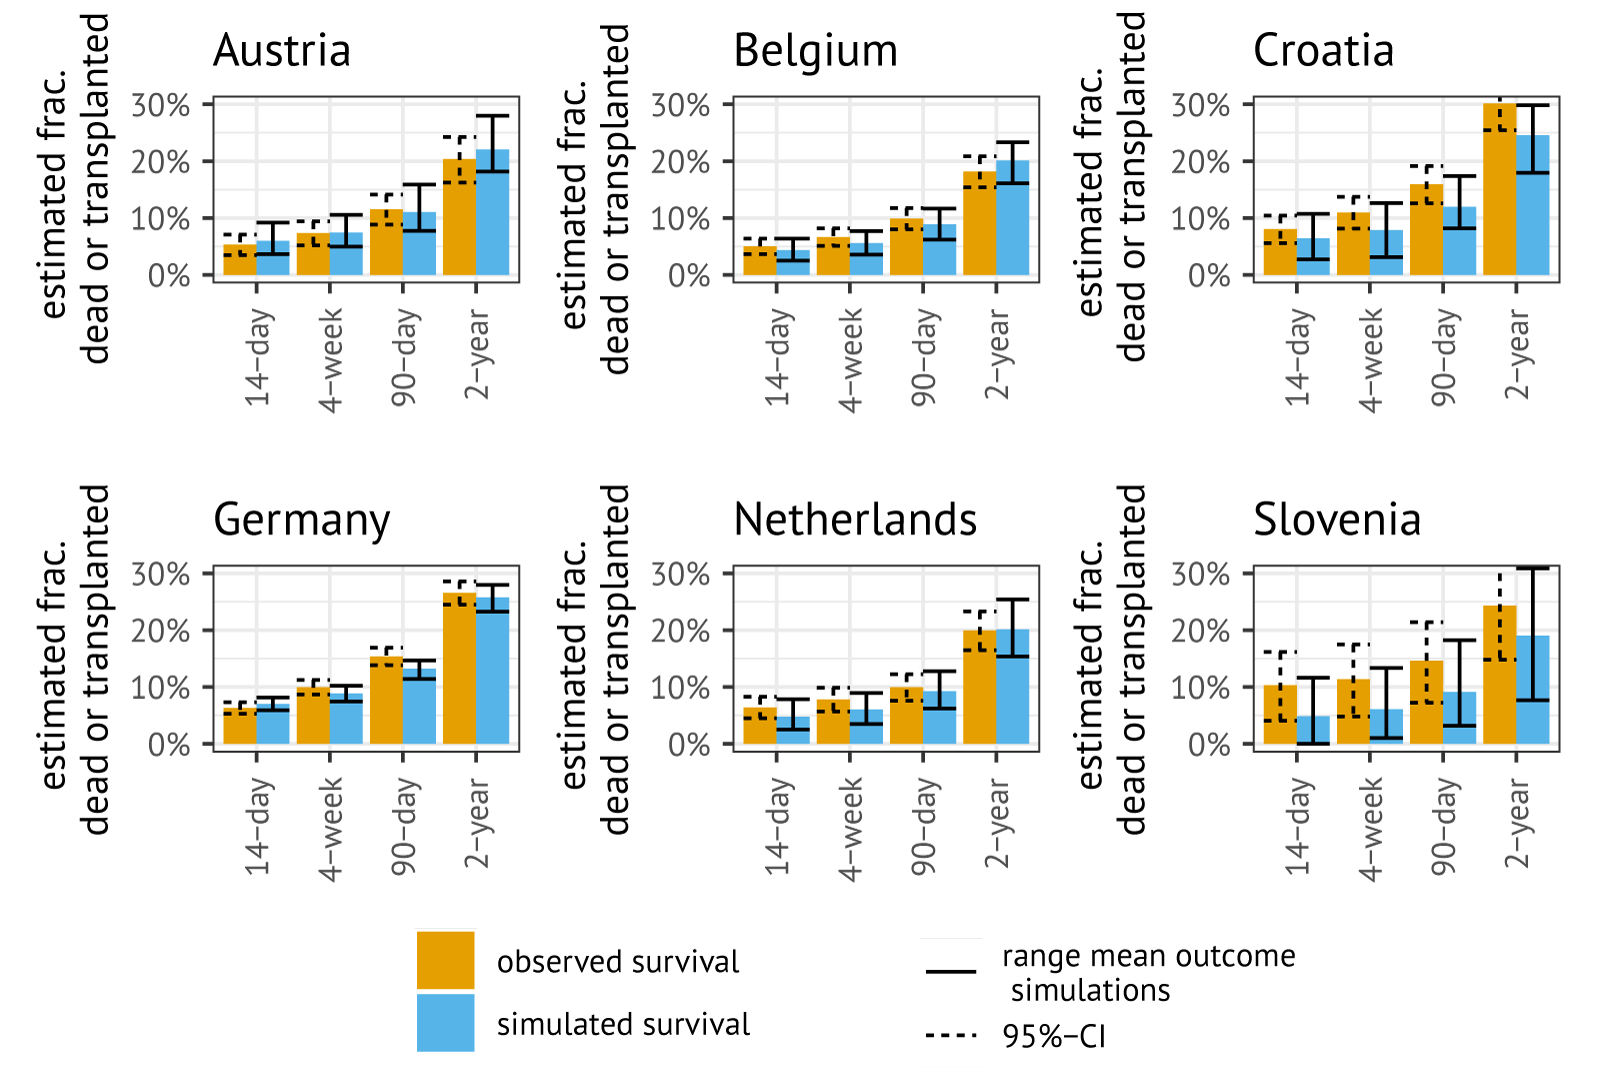
\includegraphics[width=0.9\linewidth]{figures/ch5//fig2-post_txp_event_rates} 

}

\caption{The estimated event probabilities for transplant recipients, per country for different time horizons. An event was defined as re-transplantation or waiting list death, whichever occurred first.}\label{fig:ch5fig2}
\end{figure}

\FloatBarrier

\begin{figure}[ht]

{\centering 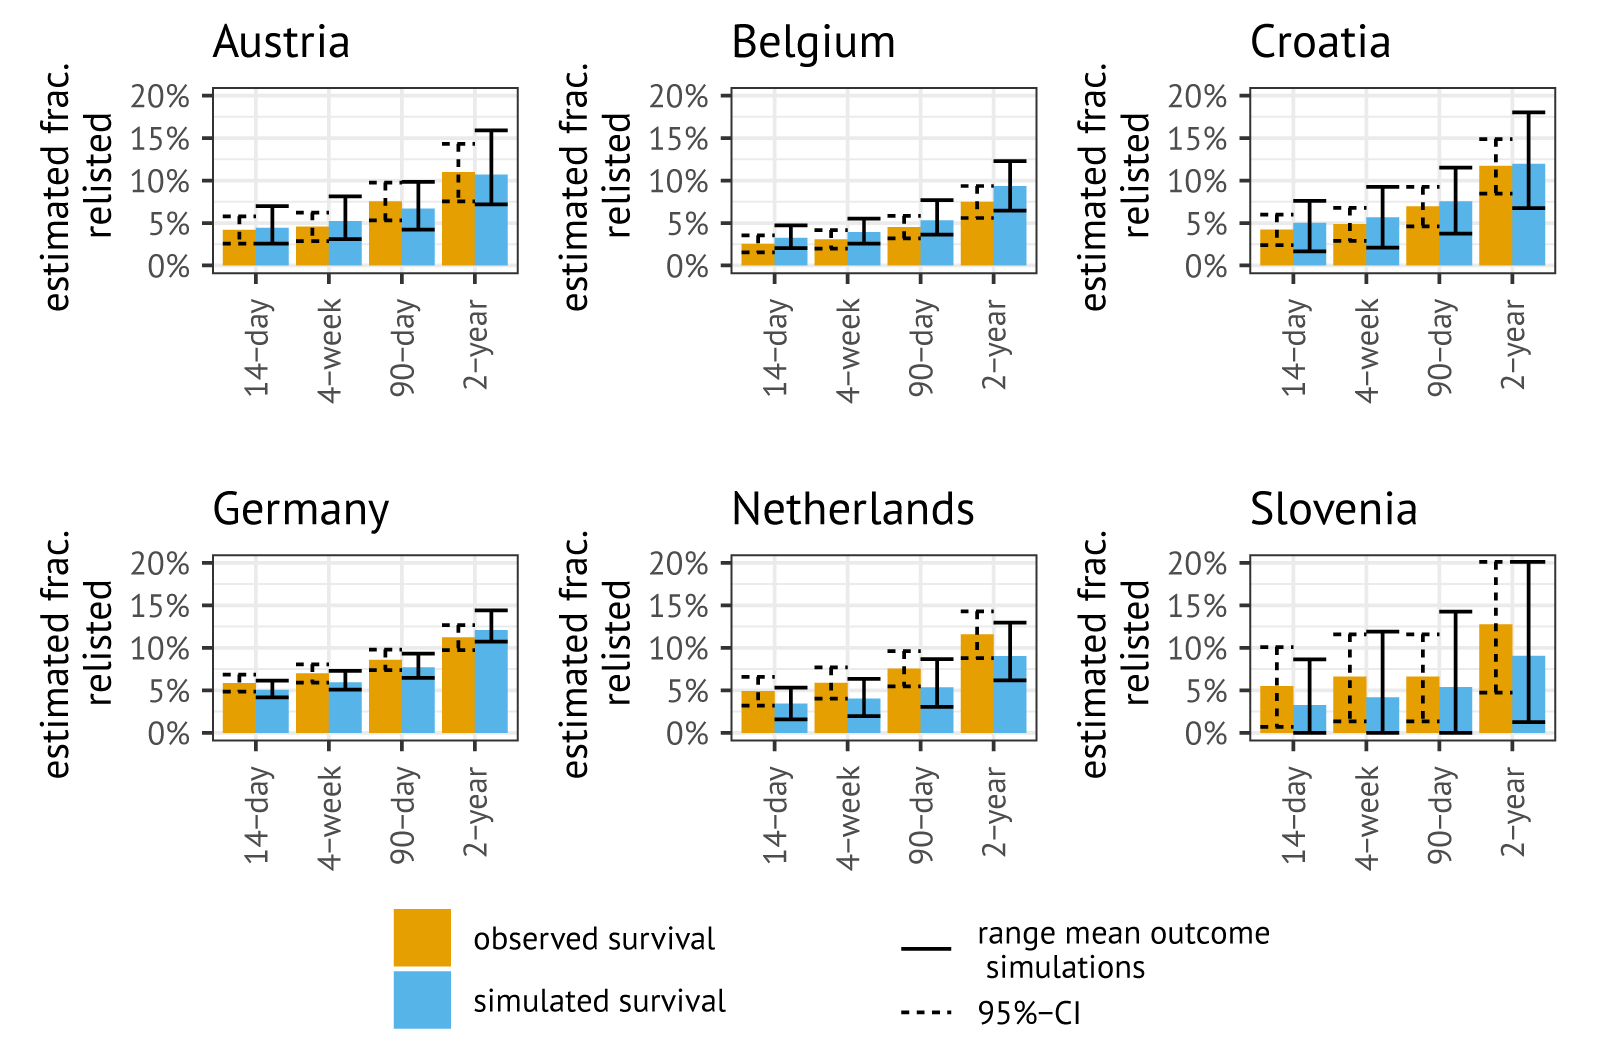
\includegraphics[width=0.9\linewidth]{figures/ch5//sfig1-post_txp_relisting_rates} 

}

\caption{Estimated re-listing rates for transplant recipients, per country for different time horizons.}\label{fig:ch5sfig1}
\end{figure}

\FloatBarrier

\subsubsection{Discussion of validation results}\label{sec:valelasdiscussion}

The ELAS simulator appears to be well-calibrated for most waiting list
and transplantation patterns within Eurotransplant. An important
exception is the total number of transplantations and waiting list exits
by lab- and match-MELD score. For example, the simulator overestimates
the total number of transplantations among candidates with high urgency
(MELD 31--40 or HU/ACO status), and underestimates the number of waiting list
deaths in this group (see Tables \ref{tab:ch5tab2} and \ref{tab:ch5tab3}).
Table \ref{tab:ch5tab3} shows that such miscalibration is present to a much
lesser degree in standard allocation, with the number of transplantations only
slightly overestimated for candidates with the highest match-MELD scores (31-40)
and the lowest lab-MELD scores (6-10).

A potential explanation for this miscalibration is that the simulator
assumes that candidates who accept a liver graft offer are always transplanted.
In practice, however, transplant centers can cancel transplantation
procedures after an initial acceptance, for example because of logistical
issues, unfavorable histopathology findings, or instability of the
transplant candidate. In such cases, Eurotransplant can re-offer
the graft to candidates who are located in the
vicinity of the graft via extended or rescue allocation. This generally
results in the placement of livers in candidates with lower urgency,
particularly in the case of rescue allocation, which operates on a first-come,
first-serve basis. We note that such rescue
allocation was not implemented for the ELAS simulator.

To assess whether competitive rescue allocation could partially explain the observed
miscalibration, we inspected the placements of the 241 liver grafts procured from
donors in the simulation period that were initially accepted by one candidate, declined
before transplantation, and then re-offered to other candidates via competitive
rescue allocation. For these 241 livers, Table \ref{tab:tabcomprescue} shows the MELD scores of
the initially accepting candidate and final transplant recipient. In general,
re-offering via rescue allocation indeed leads
to lower MELD scores at transplantation, providing a partial explanation for the
miscalibration in low-MELD groups in Table \ref{tab:ch5tab2} and \ref{tab:ch5tab3}.

A second outcome on which the simulator is not well-calibrated is the
number of transplantations per country. For example, in Belgium there
are on average 55 (+4\%) more transplantations in simulations than in
reality. This may also be explained by the lack of competitive rescue
allocation, through which approximately 10--15
grafts are transferred per year from Belgium to Germany. The fact that
too many grafts are transplanted in Belgium may also explain why the
number of transplantations in candidates with HCC is overestimated
(see Table \ref{tab:ch5tab3}), as Belgium has the highest proportion of
candidates that are listed with HCC. This seems supported by the fact that no
miscalibration is observed for the number of transplants within candidates with
HCC when restricting to livers allocated via standard allocation only
(see Table \ref{tab:ch5tab3}).

\begin{table}[h]
\caption{Priority of candidates in cases where a liver was initially accepted but later declined, and then re-allocated to a different recipient through competitive rescue liver allocation between January 1, 2016, and December 31, 2019. The table shows the number of candidates in each priority score category. For MELD scores, separate counts are included for the match-MELD score and lab-MELD score.}
\label{tab:tabcomprescue}
\centering
\resizebox{0.9\ifdim\width>\linewidth\linewidth\else\width\fi}{!}{%
\centering
\begin{tabular}{lcccc}
    \toprule
    score & \multicolumn{2}{c}{initially accepting candidate} & \multicolumn{2}{c}{final liver recipient} \\
    \midrule
    \addlinespace[0.3em]
    \multicolumn{5}{l}{\textbf{urgency category}}\\
    \hspace{.7em}HU/ACO         & \multicolumn{2}{c}{23} & \multicolumn{2}{c}{0}     \\
    \addlinespace[0.3em]
    \textbf{MELD} & match-MELD & lab-MELD & match-MELD & lab-MELD \\
    \hspace{.7em}31--40    & 60 & 38 & 1   & 0   \\
    \hspace{.7em}21--30    & 107 & 56 & 53  & 31  \\
    \hspace{.7em}11--20    & 45 & 85 & 140 & 157 \\
    \hspace{.7em}6--10     & 6  & 39 & 47  & 53  \\
    \bottomrule
\end{tabular}
}
\end{table}

\newpage
We thus have two potential explanations for miscalibration of the ELAS
simulator, which are (i) the simulator does not allow planned
transplantation procedures to be cancelled after an initial acceptance,
and (ii) the simulator does not implement competitive rescue allocation.
We have chosen not to implement these two mechanisms in the ELAS
simulator because (i) the focus of policy discussions in ELIAC is standard
allocation, not competitive rescue allocation, (ii) cancellations after an
initial acceptance are relatively rare (about 4\% of transplantations),
and (iii) the decision to proceed with rescue allocation is made on a case-by-case
basis, which is difficult to model correctly because of the limited availability
of structured data on rescue allocation. In our view, the simulated outcomes are
sufficiently close to observed outcomes to make the ELAS simulator useful
for policy evaluation. We illustrate this in Section \ref{sec:elascasestudies}
with two case studies.
\vspace*{-1em}

\section{Case studies: the impact of modifying ELAS rules}\label{sec:elascasestudies}

With two case studies, we illustrate that the ELAS simulator can be used
for quantifying the impact of liver allocation policy changes. For the first case study (Section
\ref{sec:elasbeliaccasestudy}), we
collaborated with representatives from the Belgian Liver and Intestine
Advisory committee (BeLIAC) to study the impact of changes to the
Belgian exception score system. In the second case study (Section \ref{sec:elasremeldcasestudy}), we study the
impact of basing Eurotransplant liver allocation on ReMELD-Na scores
instead of UNOS-MELD scores, which was a topic on the agenda of ELIAC in
2023.

To evaluate these ELAS policy changes, we simulate Eurotransplant liver
allocation 50 times between January 1, 2016, and December 31, 2019, and compare
the outcomes simulated under the modified ELAS rules to the outcomes simulated
under the current ELAS rules. We test whether modified policies lead to
significantly different outcomes with traditional hypothesis testing. To
increase the power of these tests, we use common random number
generators \citep{lawSimulationModelingAnalysis2015} to eliminate any variance that is
attributable to factors which we
assume to be independent from the allocation policy. Specifically, we use common random
numbers to synchronize the splitting of liver grafts, the graft offer
acceptance behavior of candidates, and the triggering of rescue
allocation across policies for each of the 50 replications. By
synchronizing these processes across policies, pairwise t-tests can be used
to establish the statistical significance of the impact of policy changes.

\subsection{Case study 1: the exception score system in Belgium}\label{sec:elasbeliaccasestudy}

Nearly half of the liver transplant candidates that are listed in Belgium
receive exception points, which makes Belgium the country with relatively
most awarded (N)SEs in Eurotransplant. Most of these (N)SEs increase with every
90 days of waiting time, which increases the match-MELD score that elective
candidates require in Belgium to be offered a liver graft. This has led to
concerns that candidates without exception points are crowded out of transplantation.

To address this, the BeLIAC has considered imposing a cap on (N)SE-MELDs
of 30, which corresponds to maximizing the awardable 90-day mortality
equivalent with a 50\% mortality equivalent. In joint discussions, the
BeLIAC also expressed an interest in capping (N)SE-MELDs at 25, as well as
alternative policy options. These alternatives were slowing down (N)SE-MELDs by
reducing the 90-day increments (referred to as ``\emph{slower}'' policies), and lowering
the initial mortality equivalents awarded for (N)SEs (referred to as
``\emph{lowered}'' policies). Table \ref{tab:ch5tab4} provides an overview
of the policy options discussed within BeLIAC.

At the request of BeLIAC, these policy alternatives were evaluated with the
ELAS simulator. Figure \ref{fig:ch5fig3} and
Table \ref{tab:ch5tab5} summarize the results, which both focus on livers
from DBD donors (DCD donors are center offers in Belgium). Figure
\ref{fig:ch5fig3} visualizes the distributions of the simulated
(N)SE-MELD scores at DBD transplantation for exception candidates (left),
and laboratory MELD scores at DBD transplantation for non-exception
candidates (right). The figure shows that capping (N)SE-MELDs at 30
barely affects their distribution at transplantation, while the other
policy alternatives reduce the median (N)SE-MELD at transplantation by up to 4 points
on the MELD scale (left side).
It also shows that lab-MELD scores at DBD transplantation for non-exception
candidates become lower when (N)SEs are capped (right side). In fact,
the median lab-MELD at DBD transplantation
becomes up to 3 MELD points lower with \emph{slower} and \emph{lowered} policies, than the median observed under the current allocation rules. These alternative policies thus increase access to
transplantation for candidates with lab-MELD scores between 20 and 23,
which may be desired as they face a 90-day
mortality risk between 10 to 15\%.

\newpage

\begin{table}[h]
\caption{Policy options for the Belgian (N)SE system. Modifications are applied only to all Belgian SEs and the NSE, and not to the PED-MELD score as PED-MELD scores are valid internationally. A dash (-) indicates that the policy did not change an (N)SE attribute.}
\label{tab:ch5tab4}
\centering
\resizebox{1\ifdim\width>\linewidth\linewidth\else\width\fi}{!}{%
\begin{tabular}{C{.18\linewidth} C{.35\linewidth} C{.3\linewidth} C{.28\linewidth}}
    
    %{p{.158\linewidth}p{.35\linewidth}p{.3\linewidth}p{.28\linewidth}}
        \toprule
        \rowcolor[HTML]{FFFFFF} 
        policy option        & initial   equivalent                                                                  & 90-day   increment                            & maximum mortality  equivalent \\ \midrule
        \rowcolor[HTML]{EFEFEF} 
        current & 10\% (MELD 20) for most (N)SEs, 15\%  (MELD 22) for HCC                                                    & 10\%     (2-4 MELD points)                  & 100\%                \\
        \rowcolor[HTML]{FFFFFF} 
        capped (25)  & -  & - & 25\%$^a$ (MELD 25)     \\
        \addlinespace[0.3em]
        \rowcolor[HTML]{FFFFFF} 
        capped   (30) & - & - & 50\%$^a$   (MELD 30)   \\[.1em]
        \rowcolor[HTML]{EFEFEF} 
        slower        & - & 5\%       (1-2 MELD points)                 & -                    \\[0.3em]
        \rowcolor[HTML]{EFEFEF} 
        slowest       & - & 2.5\%   (1 MELD point)                      & -                    \\
        \rowcolor[HTML]{FFFFFF} 
        lowered       & lowered to 8\% (MELD 18) for existing (N)SEs with initial equivalents \textless{}20\% & -                                           & -                    \\ \bottomrule
    \end{tabular}
}
\parbox{\textwidth}{\footnotesize \smallskip $^a$Set to the initial equivalent if the initial equivalent exceeds the proposed cap. For example, candidates with biliary atresia maintain a 60\% mortality equivalent.}
\end{table}

\begin{figure}[ht]

{\centering 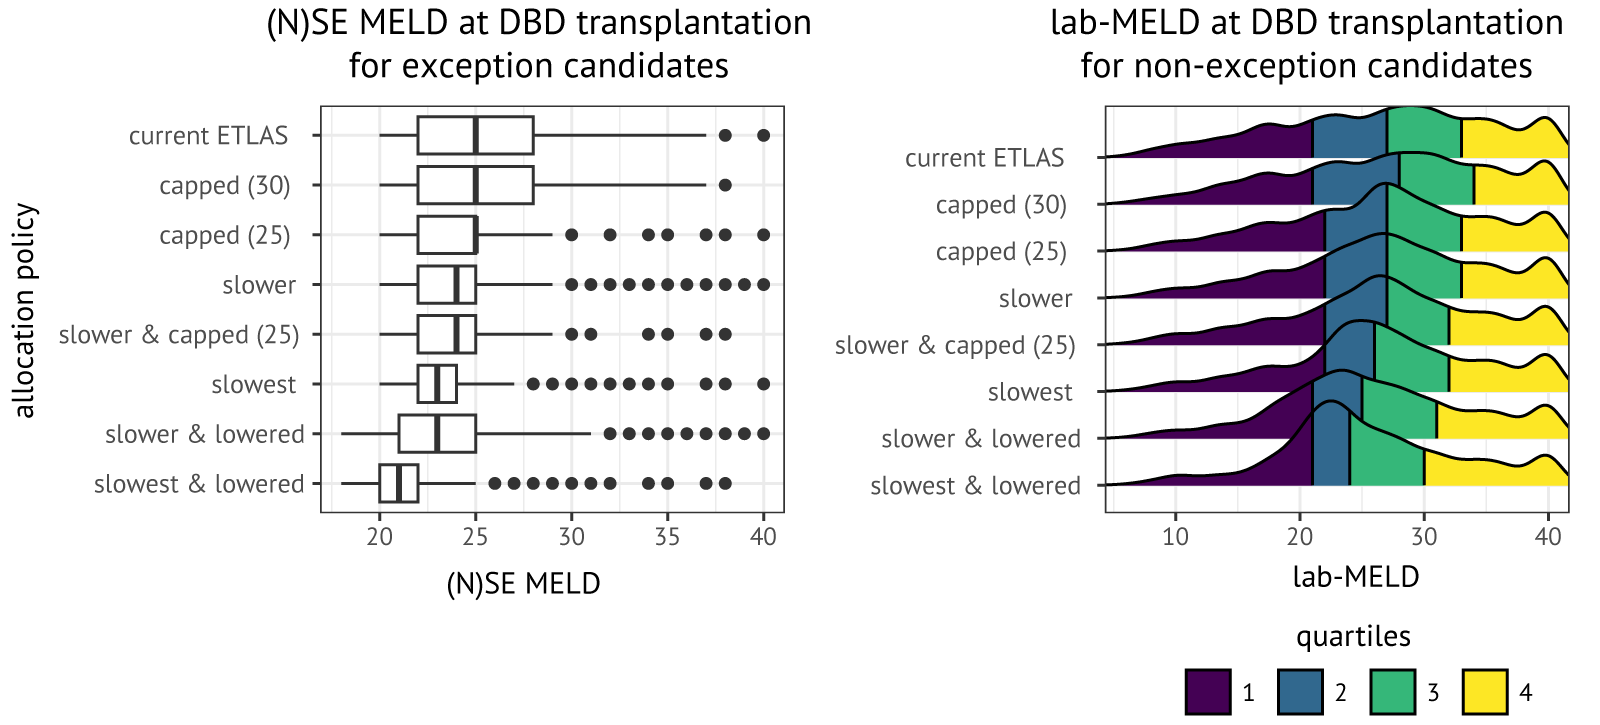
\includegraphics[width=1\linewidth]{figures/ch5//fig3-results_BELIAC} 

}

\caption{Distribution of (N)SE MELD scores at transplantation for exception candidates (left) and laboratory MELD scores at transplantation for non-exception candidates (right) in ELAS simulations. Only transplantations that were the result of patient-driven allocation are shown. Boxplots and distributions were calculated over 50 simulations.}\label{fig:ch5fig3}
\end{figure}

\FloatBarrier
\newpage
Table \ref{tab:ch5tab5} shows summary statistics for the simulated waiting list outcomes,
separately for exception and non-exception candidates. Comparing the third column (actual 2016-2019 statistics) to
the fourth column (averages and 95\% IQRs over the 50 simulations) shows that
the ELAS simulator is well-calibrated for the number of
transplantations, waiting list deaths, and waiting list exits. This
reassures us that the ELAS simulator reasonably describes these
allocation patterns. Of policy interest are the remaining columns of
Table \ref{tab:ch5tab5}, which show for every (N)SE policy alternative
the average number of events over the 50 simulations. Comparing
these outcomes to the outcomes simulated under current (N)SE rules shows
that almost all policies significantly change the number of
transplantations, the number of waiting list deaths, and the number of
waiting list removals.

The greatest effects are sorted by combining the \emph{slowest} and \emph{lowered} policies
(final column), with which on average 20 (+5\%) extra candidates without exception
points are transplanted. According to the simulation results, this policy could
have avoided 12 waiting list deaths in non-exception candidates in Belgium (-10\%),
which corresponds to 3 waiting list deaths per year. The cost of this policy change
is that we see a slight increase in the number of waiting list removals for
exception patients, with on average 1--2 extra exception patients per year
removed because they became unfit for transplantation, or because they had HCC
or another form of cancer.

\begingroup
\sisetup{range-phrase = {\,\textemdash\,}}

\begin{table}[h]
\caption{Waiting list exits for elective candidates in Belgium between January 1, 2016, and January 1, 2020. The numbers displayed are the average number of exits over 50 simulations. Scenarios modifying the allocation rules were compared to simulations under the current ELAS rules with pairwise t-tests.}
\label{tab:ch5tab5}
\centering
\resizebox{1\ifdim\width>\linewidth\linewidth\else\width\fi}{!}{%
\begin{tabular}{C{.18\linewidth}C{.10\linewidth}C{.09\linewidth}C{.19\linewidth}C{.10\linewidth}C{.10\linewidth}C{.09\linewidth}C{.15\linewidth}C{.10\linewidth}C{.11\linewidth}C{.11\linewidth}}
    \toprule
    exit reason & \makecell{patient\\type} & \makecell{current\\ (real)} & \makecell{current\\ (sim)} & \makecell{capped\\(30)} & \makecell{capped\\(25)} & slower & \makecell{slower \&\\ capped (25)} & slowest & \makecell{slower \&\\ lowered} & \makecell{slowest \&\\ lowered}\\
\midrule
 & (N)SE & 438 & \phantom{}\num{450} [\numrange{428}{470}] & 445 & 448 & 443*** & 445* & 440*** & 438*** & 433***\\

\multirow{-2}{*}{\raggedright\arraybackslash transplanted} & None & 387 & \phantom{}\num{405} [\numrange{379}{423}] & 406* & 408** & 412*** & 409*** & 413*** & 420*** & 425***\\
\cmidrule{1-11}
 & (N)SE & 27 & \phantom{0}\num{27} [\numrange{19}{40}] & 28 & 27 & 28 & 29 & 29* & 29 & 29*\\

\multirow{-2}{*}{\raggedright\arraybackslash \makecell{waiting list\\death}} & None & 119 & \phantom{}\num{126} [\numrange{108}{141}] & 126 & 122** & 122* & 122** & 117*** & 116*** & 114***\\
\cmidrule{1-11}
 & (N)SE & 20 & \phantom{0}\num{14} [\numrange{8}{17}] & 14 & 14* & 14** & 14* & 15*** & 16*** & 17***\\

\multirow{-2}{*}{\raggedright\arraybackslash unfit} & None & 23 & \phantom{0}\num{21} [\numrange{16}{29}] & 21 & 20 & 21 & 20 & 20 & 20 & 20*\\
\cmidrule{1-11}
 & (N)SE & 8 & \phantom{00}\num{8} [\numrange{5}{16}] & 9 & 10** & 10** & 11*** & 11*** & 11*** & 13***\\

\multirow{-2}{*}{\raggedright\arraybackslash \makecell{removed\\HCC or Cancer}} & None & 6 & \phantom{00}\num{6} [\numrange{2}{14}] & 6 & 6 & 6 & 6 & 6 & 6 & 6\\
\bottomrule
\end{tabular}
}
\parbox{\textwidth}{\footnotesize \smallskip $^{*}$ p < 0.05, $^{**}$ p < 0.01, $^{***}$ p < 0.001}
\end{table}

\endgroup

\FloatBarrier
\vfill

\subsection{Case study 2: basing Eurotransplant liver allocation on ReMELD-Na}\label{sec:elasremeldcasestudy}

Candidates with hyponatremia, i.e.~low serum sodium levels, face systematically
higher waiting list mortality rates than suggested by
their MELD score \citep{kimHyponatremiaMortalityPatients2008a}. To adequately
prioritize these patients, MELD-Na was introduced in 2016 for liver allocation
in the United States. In 2020, Goudsmit et aFl. revised this MELD-Na score with retrospective
data from Eurotransplant, leading to the \emph{ReMELD-Na} score.

In May 2023, the ELIAC recommended basing Eurotransplant liver allocation
on ReMELD-Na instead of UNOS-MELD. A matter of concern for ELIAC was
that ReMELD-Na scores range from 1 to 36, while UNOS-MELD scores range
from 6 to 40. Basing laboratory MELD scores on ReMELD-Na without
updating the MELD-curve could therefore mean that non-exception
candidates -- who depend on lab-MELD for access to transplantation -- could
only receive match-MELD scores up to 36, while candidates with (N)SE
or PED-MELD scores could still receive match-MELD scores up to 40. A
switch to ReMELD-Na could thereby inadvertently give extra priority to
candidates with exception points, who already appear to have an advantage in ELAS
\citep{umgelterDisparitiesEurotransplantLiver2017a}.

To support this discussion, we simulated two scenarios for liver allocation using
ReMELD-Na. For both scenarios, lab-MELD scores were based on ReMELD-Na, calculated
using:

\[
\begin{aligned}
\text{ReMELD-Na} &= 7.85 + 9.03\ln(\text{crea}) + 2.97\ln(\text{bili}) + 9.52\ln(\text{INR}) + \\
& 0.392(138.6 - \text{Na}) - 0.351(138.6 - \text{Na})\ln(\text{crea}).
\end{aligned}
\]

In the first scenario, the exception score system remained unchanged,
which means that PED-MELD and (N)SE-MELD scores are calculated based on
the UNOS-MELD survival curve. This curve is given by the following
formula:

\[
S_{90}^{\texttt{UNOS-MELD}} = 0.98037^{0.17557(\texttt{UNOS-MELD} - 10)}.
\]

In the second scenario, PED-MELD and (N)SE-MELD scores are instead
calculated based on a survival curve developed specifically for
ReMELD-Na. This curve was obtained by estimating a Cox proportional hazards
model on Eurotransplant registry data using ReMELD-Na as the only covariate.
The obtained ReMELD-Na curve is given by the following formula:

\[
S_{90}^{\text{ReMELD-Na}} = 0.9745^{0.2216(\text{ReMELD-Na} - 10)}.
\]

\newpage
Table \ref{tab:ch5tab6} shows simulated waiting list outcomes under
these ReMELD-Na policies, summarized over 50 simulations. The
third column shows that introducing ReMELD-Na without updating the
S-curve results in approximately 70 extra waiting list deaths in total
(p \textless{} 0.001), which corresponds to 15--20 extra waiting list deaths per
year. This finding is likely explained by ELIAC's concern that a switch
to ReMELD-Na inadvertently deprioritizes candidates who depend on
lab-MELD scores for access to transplantation. The fourth column shows
that switching to ReMELD-Na with the updated S-curve could have averted
25 waiting list deaths in total (p \textless{} 0.001).

\begin{table}[h]
\caption{Average number of simulated waiting list exits for candidates under UNOS-MELD and ReMELD-Na, with and without updating the S-curve. The numbers in brackets are 95\% interquantile ranges, observed over 50 simulations of ELAS between January 1, 2016, and January 1. Paired t-tests were used to test whether either scenario significantly affected the simulated waiting list outcomes.}
\label{tab:ch5tab6}
\centering
\resizebox{1\ifdim\width>\linewidth\linewidth\else\width\fi}{!}{%

\begin{tabular}{lccc}
    \toprule
    exit status & \makecell{UNOS-MELD\\(current)} & \makecell{ReMELD-Na\\(old S-curve)} & \makecell{ReMELD-Na\\(updated S-curve)}\\
    \midrule
    waiting list deaths & 1633.4 [1581.2-1685.6] & 1703.3*** [1643.2-1763.3] & 1608.3*** [1546.9-1669.7]\\
    transplantations & 6414.5 [6400.1-6428.9] & 6417.7* [6401.6-6433.7] & 6410.3*** [6396.7-6423.8]\\
    removed & 859.9 [834.8-885] & 837.9*** [812.9-862.8] & 870.4*** [842.7-898.1]\\
    \bottomrule
\end{tabular}
}
\parbox{\textwidth}{\footnotesize \smallskip $^{*}$ p < 0.05, $^{**}$ p < 0.01, $^{***}$ p < 0.001}
\end{table}

An important limitation of this analysis is that serum sodium
measurements are not available for most candidates in Eurotransplant
registry data. When serum sodium was missing in simulations, we
calculated ReMELD-Na scores with a serum sodium level of 138.6 mmol/l,
which results in 0 points being awarded for hyponatremia. Because this
means that hyponatremia could not be prioritized in all
candidates, the reduction of 25 waiting list deaths is a
conservative projection.

Whether serum sodium is reported to Eurotransplant depends primarily on
the candidate's listing center, because the transplant centers either never or
almost always report serum sodium to Eurotransplant. This motivated us to also assess
the number of waiting list deaths stratified by the listing center's track record of reporting serum sodium. For this, we
categorize centers into centers with high, medium and low serum sodium
completeness. Table
\ref{tab:ch5tab7} shows the total number of
waiting list deaths per type of center. It can be seen that the
reduction in waiting list deaths is indeed concentrated in centers with
high serum sodium completeness, with 28 fewer waiting list deaths observed
in such centers. Under the (optimistic) assumption that this reduction in
waiting list deaths is representative for all centers in Eurotransplant,
using ReMELD-Na as the basis for liver allocation could have prevented
up to 80 waiting list deaths over the simulation period.

\begin{table}[h]
\caption{Simulated number of waiting list deaths for candidates between January 1, 2016, and January 1, 2020, under UNOS-MELD (current) and ReMELD-Na with an updated S-curve.}
\label{tab:ch5tab7}
\centering
\resizebox{1\ifdim\width>\linewidth\linewidth\else\width\fi}{!}{%

\begin{tabular}{C{.20\linewidth}C{.10\linewidth}C{.10\linewidth}C{.32\linewidth}C{.32\linewidth}}
\toprule
\makecell{serum sodium\\completeness} & \makecell{center\\count} & \makecell{patient\\count} & \makecell{waiting list deaths \\under UNOS-MELD} & \makecell{waiting list deaths \\under ReMELD-Na}\\
\midrule
high & 14 & 3995 & 589.3 [554.8-623.9] & 561*** [518.6-603.4]\\
medium & 13 & 3098 & 446.9 [404-489.7] & 446.9 [402.1-491.7]\\
low & 10 & 4775 & 590.3 [551.3-629.3] & 593.8 [555.3-632.4]\\
\bottomrule
\end{tabular}
}
\parbox{\textwidth}{\footnotesize \smallskip high: serum sodium known for >75\% of candidates; medium: serum sodium known for >50\% of candidates; low: otherwise.\\ $^{*}$ p < 0.05, $^{**}$ p < 0.01, $^{***}$ p < 0.001}
\end{table}

\FloatBarrier

In discussions with ELIAC and national competent authorities on ReMELD-Na,
concerns were raised about the impact of ReMELD-Na on pediatric,
adolescent, and female transplant candidates. Table \ref{tab:ch5tab8}
shows the simulated impact of ReMELD-Na on these vulnerable patient groups. The switch
to ReMELD-Na has little impact on outcomes for these patients, suggesting that
the reduction in waiting list deaths is concentrated in males aged 30
years or older.

The table also shows the impact of ReMELD-Na on candidates with renal dysfunction:
fewer candidates on biweekly dialysis are transplanted under ReMELD-Na, as are
candidates who require a combined liver and kidney transplantation. Such a change
could potentially be welcomed, as there are indications in the literature that
UNOS-MELD overprioritized candidates with renal dysfunction \citep{sharmaReweightingModelEndStage2008}.

\begin{table}[!h]
\centering
\caption{\label{tab:ch5tab8}Averages of the simulated number of waiting list exits per vulnerable patient group based on simulation of ELAS between January 1, 2016 and December 31, 2019.}
\centering
\resizebox{\ifdim\width>\linewidth\linewidth\else\width\fi}{!}{
\fontsize{9.5}{11.5}\selectfont
\begin{tabular}[t]{>{\centering\arraybackslash}p{2cm}ccccc}
\toprule
  &   & UNOS-MELD & ReMELD-Na & diff. & per year\\
\midrule
 & transplanted & 220 \mbox{[205-235]} & 209 \mbox{[196-220]} & -11 & -2.8\\
\cmidrule{2-6}
\multirow{-2}{2cm}[1\dimexpr\aboverulesep+\belowrulesep+\cmidrulewidth]{\centering\arraybackslash pediatric cand. (<18 yrs)} & deceased & 24 \mbox{[20-28]} & 25 \mbox{[20-31]} & 1 & 0.2\\
\cmidrule{1-6}
 & transplanted & 232 \mbox{[216-247]} & 219 \mbox{[206-232]} & -13 & -3.3\\
\cmidrule{2-6}
\multirow{-2}{2cm}[1\dimexpr\aboverulesep+\belowrulesep+\cmidrulewidth]{\centering\arraybackslash adolescents (18-29 yrs)} & deceased & 25 \mbox{[21-29]} & 27 \mbox{[21-33]} & 2 & 0.5\\
\cmidrule{1-6}
 & transplanted & 1599 \mbox{[1562-1637]} & 1586 \mbox{[1557-1614]} & -13 & -3.3\\
\cmidrule{2-6}
\multirow{-2}{2cm}[1\dimexpr\aboverulesep+\belowrulesep+\cmidrulewidth]{\centering\arraybackslash females} & deceased & 524 \mbox{[497-551]} & 522 \mbox{[500-544]} & -2 & -0.5\\
\cmidrule{1-6}
 & transplanted & 236 \mbox{[225-246]} & 204 \mbox{[192-217]} & -32 & -8.0\\
\cmidrule{2-6}
\multirow{-2}{2cm}[1\dimexpr\aboverulesep+\belowrulesep+\cmidrulewidth]{\centering\arraybackslash liver + kidney candidates} & deceased & 57 \mbox{[50-64]} & 68 \mbox{[59-77]} & 11 & 2.8\\
\cmidrule{1-6}
 & transplanted & 442 \mbox{[414-470]} & 376 \mbox{[352-401]} & -66 & -16.5\\
\cmidrule{2-6}
\multirow{-2}{2cm}[1\dimexpr\aboverulesep+\belowrulesep+\cmidrulewidth]{\centering\arraybackslash candidates on dialysis} & deceased & 257 \mbox{[237-276]} & 275 \mbox{[253-297]} & 18 & 4.5\\
\bottomrule
\end{tabular}}
\end{table}

\FloatBarrier
\vfill
\newpage

\section{Conclusions and discussion}\label{sec:elasconclusion}

To help align the interests and perspectives of its member countries,
Eurotransplant requires a tool that can quantify the impact of proposed policy
changes to its liver allocation system. Discrete-event simulation is an excellent tool for this purpose, and
is already routinely used in other geographic regions to revise organ allocation
policies. This chapter reports on the development of the ELAS simulator, which is the first simulator
tailored to the unique challenges of Eurotransplant as a multi-national
organ exchange organization.

To build trust in the ELAS simulator as a policy evaluation tool, we
have validated the ELAS simulator by comparing simulated outcomes to
observed outcomes between January 1, 2016, and December 31, 2019. We found
that the simulator is able to closely replicate most
patterns in Eurotransplant liver allocation. In our own view, and in ELIAC's, the remaining differences are sufficiently small for the
ELAS simulator to contribute to liver allocation policy evaluation
within Eurotransplant. We have illustrated this with two case studies.
The case study on the Belgian exception point system has been discussed within
BeLIAC, and has led to a recommendation to cap (N)SE scores in Belgium at 28.
The case study on ReMELD-Na has led to a recommendation to switch to allocation
based on ReMELD-Na, which was implemented on March 25, 2025.

Although this demonstrates that the ELAS simulator is useful for policy
evaluation, the software also has limitations. A first limitation is that our
simulations are driven by Eurotransplant registry data, which does not capture all information relevant
for liver allocation development. For example, in the second case study we have seen that
serum sodium is not available in Eurotransplant registry data for many candidates, which
complicated the assessment of the impact of allocation based on ReMELD-Na. This limitation could be addressed by prospective
data collection of factors relevant to allocation. Secondly, the statistical models
for graft offer acceptance behavior and post-transplant survival were calibrated
to historical data. Developments in liver transplantation threaten the external validity of
these models. An example of such a development is machine perfusion,
which is enhancing the outcomes after liver transplantation
\citep{terraultLiverTransplantation20232023} and which is altering the graft offer
acceptance behavior of transplant centers. This limitation can
potentially be addressed by re-calibrating the statistical models with
contemporary data.

From a policy perspective, several areas remain in which
Eurotransplant's liver allocation system may be improved. These areas
include taking post-transplant outcomes into account when allocating
livers \citep{Allen2024}, broader geographic sharing of livers for candidates
with very high MELD scores
\citep{massieEarlyChangesLiver2015, Ravaioli2022}, and
rectifying sex disparity in liver waiting list outcomes
\citep{deFerranteSexDisparityLiver2024}. We anticipate that the ELAS simulator can
play a role in informing ELIAC of the impact of policy changes
related to these topics.

\part{Allocation of the kidney}

\chapter{Kidney allocation in Eurotransplant}\label{CHprefacekidney}

Up to 100 million Europeans have Chronic Kidney Disease (CKD) \citep{Vanholder2021}.
CKD is characterized by the progressive loss of kidney function, and its causes
include diabetes, hypertension, and glomerulonephritis. Patients with CKD
can eventually progress to End-Stage Renal Disease (ESRD), which means that they
become dependent on renal replacement therapies (RRTs) such as dialysis or
kidney transplantation. Whereas other forms of end-stage organ failure cannot
be managed with therapy, end-stage kidney failure can be managed for extended
periods with dialysis \citep{HaaseKromwijk1999}.
However, kidney transplantation is the preferred treatment option for most
patients with ESRD because it is associated with a reduction in patient mortality
and improves the patient's quality of life \citep{Tonelli2011}.

Kidney transplantation became the preferred treatment option for patients with
ESRD in the 1980s, when substantial improvements were observed in post-transplant
outcomes \citep{HaaseKromwijk1999}. As a result, the kidney waiting list in Eurotransplant
expanded from less than 2,000 patients in 1980
to approximately 10,500 patients in 1994 \citep{eurotransplantAR2005}. Since then, the number of patients awaiting kidney transplantation has remained stable in
Eurotransplant with approximately 10,000 patients currently waiting for a kidney transplant.

Eurotransplant allocates kidneys from deceased-organ donors to these waiting patients.
When Eurotransplant was initiated, candidates were prioritized solely based
on Human Leucocyte Antigen (HLA) matching. Currently,
Eurotransplant uses an allocation system which tries to balance HLA matching
with fairness considerations. In this chapter, we describe the history of this
system and some contemporary challenges in the allocation of deceased-donor kidneys.
We also briefly describe the work included in this thesis that can inform
discussions on addressing these challenges.

\section{HLA matching versus fairness}\label{hla-matching-versus-fairness}

In the late 1960s, immunologists observed that the best outcomes after kidney
transplantation were observed in pairs of siblings who had compatible ABO blood groups
and matching leukocyte antigen groups \citep{vanDorp2001}. Anticipating that
such a matching effect also existed when transplanting kidneys from deceased donors,
Jon van Rood proposed Eurotransplant, a program in which a central office
would use a computer to locate the best-matching candidate for the kidneys that
became available from deceased donors \citep{vanRoodET1967}.
Shortly after Eurotransplant was initiated in 1967, similar organizations were
established in other geographic regions, motivated by the idea that outcomes after
deceased-donor transplantation could only be improved through collaboration \citep{bakJensenShareNotShare2008}.

Already in 1970, this idea became controversial with a strong debate emerging between
immunologists and clinicians on the actual importance of leukocyte-antigen
matching in deceased-donor kidney transplantation \citep{daussetHLAStory1995, vanRood2004}.
The commitment of immunologists to HLA matching was strengthened in the 1970s
and 1980s, as they unraveled many complexities of what became known
as the Human Leucocyte Antigen (HLA) system. The discovery of HLA-DR antigens in 1977
was particularly important, as these antigens were shown to have a stronger effect
on prognosis after kidney transplantation than the earlier discovered HLA-A
and HLA-B antigens \citep{Persijn1978, Persijn1981, bakJensenShareNotShare2008}.

At the same time, it was recognized that HLA matching was far from a magic bullet;
many patients with poorly matched kidneys had good outcomes after
transplantation \citep{terasaki1990history, vanRood2004}. Based on such observations,
clinicians questioned whether HLA matching was worth the effort, especially because
the practice resulted in disparities in access to transplantation \citep{Kjellstrand1988}.
For example, in the United States, it was observed that black patients were waiting
three times longer than white patients for a kidney transplant.
Thomas Starzl, who is known as ``the father of modern transplantation'', criticized the blind focus
on HLA matching in kidney allocation, referring to it as \emph{``the institutional
organization of racial bias''} \citep[159]{vanDorp2001}. To reduce such disparities,
Starzl's transplant center instead used a point system to prioritize candidates
for transplantation, in which tissue matching played a role that was
\emph{``significant but far from overriding''} \citep{starzlMultifactorialSystemEquitable1987}.

This criticism of HLA matching intensified in the 1980s with the advent of cyclosporine
A. This immunosuppressant strongly reduced the incidence of acute rejection of kidney
transplants, and was responsible for the major improvements in kidney transplant
outcomes that were observed in the 1980s. Shortly after the introduction of
cyclosporine A, several single-center studies
suggested that this immunosuppressant had made HLA matching in kidney transplantation
redundant \citep{greensteinEvidenceThatZero1990, harfmannRenalTransplantationUsing1989}.
These early findings have since been contradicted by multi-center and
registry-based studies, which showed that HLA matching continues to be strongly
associated with graft and patient survival \citep{opelzCORRELATIONHLAMATCHING1985, Opelz2007}.
\newpage
Based on these later studies, consensus has arisen that the best outcomes are observed
in patients who receive transplants with zero mismatches on the HLA-A, HLA-B,
and HLA-DR loci \citep{opelzCORRELATIONHLAMATCHING1985, morrisAnalysisFactorsThat1999}. However,
the extensive polymorphism of the HLA system means that perfectly matched kidneys
are not available for most candidates. In fact, it was already known in the 1980s
that only about one in five patients can receive a perfectly matched kidney
with a waiting list of 10,000 patients \citep{CICCIARELLI1987}. Most patients
thus have to settle for a kidney with HLA mismatches. In that case, consensus is
that HLA-DR matching is more important than HLA-B matching, which in turn is more
important than HLA-A matching \citep{Ting1985, joyseyTissueTypingPolicy1989, thorogood1990}.

Because of the role of HLA matching was contended, kidney allocation first
became more decentralized in the 1980s \citep{bakJensenShareNotShare2008}. For example,
in 1988 Eurotransplant introduced a kidney allocation system that mandated
exchange of kidneys between centers only for (a) patients who had zero HLA mismatches
with the kidney and (b) the so-called ``\emph{hyper-immunized patients}'' (see Section \ref{sec:introam})
\citep{HaaseKromwijk1999}. Otherwise, the center responsible for procurement of the kidneys
could choose patients from their own waiting list for transplantation, subject to blood group
compatibility rules and minimum HLA match criteria (defined as 2 DR matches, or
1 B + 1 DR match) \citep{HaaseKromwijk1999}. Procurement centers also had the option to
voluntarily offer the kidneys to the Eurotransplant pool. Candidates would then be prioritized by
compatibility at the HLA-DR locus, followed by compatibility at the HLA-B locus,
and finally compatibility at the HLA-A locus \citep{HaaseKromwijk1999}.

When Eurotransplant evaluated this system in the 1990s, concerns were raised
over the fact that (i) 10 percent of patients consistently waited more than five years
for kidney transplantation, (ii) transplant rates were low for candidates with
rare HLA types or homozygosity at any of the HLA loci, and (iii) procurement
and transplant rates were imbalanced between the centers and countries
\citep{DeMeester1998_booksection}. These fairness concerns
eventually led to the adoption of the Eurotransplant Kidney Allocation System
(ETKAS) in 1996, which was based on a point system that had been proposed by
Wujciak and Opelz in the years before. Besides this program, Eurotransplant
has used two other programs to allocate deceased-donor kidneys since the 1990s:
the Acceptable Mismatch (AM) program for the allocation of kidneys to hyper-immunized candidates (Section
\ref{sec:introam}), and the Eurotransplant Senior Program (ESP) for the allocation
of kidneys from donors aged 65 years or older (Section \ref{sec:introesp}).

\newpage

\section{Kidney allocation programs in Eurotransplant}\label{kidney-allocation-programs-in-eurotransplant}

\subsection{The Eurotransplant Kidney Allocation System (ETKAS)}\label{the-eurotransplant-kidney-allocation-system-etkas}

Wujciak and Opelz tried to address the dilemma between HLA
matching and fairness by using computer simulations to develop a point system
for kidney allocation \citep{wujciakProposalImprovedCadaver1993a, Opelz1998}. This
system awarded points for the absence of HLA mismatches, but also points for
a candidate's waiting time to ensure that no candidate would be left behind.
Additionally, to avoid extreme waiting times for difficult-to-match patients,
the system awarded points for the \emph{``mismatch probability''}, a quantification of
how common favorably matched kidneys are for the patient.

Eurotransplant implemented a modified version of this point system for kidney
allocation in 1996, and the resulting program has become known as the
Eurotransplant Kidney Allocation System (ETKAS) program. The modifications made
included that ETKAS awards extra priority to pediatric candidates, and implements
a mechanism to balance the international transfer of kidneys \citep{Opelz1998}.

One year after the introduction of ETKAS, in 1997, it was concluded that ETKAS
successfully achieved its primary goals; the system had increased the number of transplantations
among pediatric and long-waiting candidates and it had corrected imbalances in
the international exchange of kidneys \citep{demeesterNewEurotransplantKidney1998, Persijn2006}.
Despite this apparent success, it was also pointed out by Wujciak and Opelz that
ETKAS \emph{``could not be considered a final and unalterable product''}, which instead
would require \emph{``continued fine-tuning depending on new developments''} \citep{Opelz1998}.

In light of these comments, it is not surprising that several refinements have
been made to ETKAS since 1996. One refinement concerns the definition of
waiting time. When ETKAS was initiated, waiting time was defined as the number of days
a candidate had spent on the waiting list, which conferred an advantage to patients
who were referred early to the kidney waiting list. To address this, Eurotransplant
redefined waiting time to the number of days a candidate had received dialysis
in January 2000 \citep{DeMeester2000}. A second issue was that ABO
blood group O kidneys could be transplanted in non-O candidates in case of
a zero mismatch, which led to an increased waiting list mortality and longer
waiting times for blood group O patients \citep{glander2010}. In June 2010, this
issue was addressed by always requiring candidates and donors to have identical
ABO blood groups in ETKAS.

Shortcomings of ETKAS have also been identified for which an adequate solution
has remained elusive. A notable example is that the ETKAS point system places
equal emphasis on the HLA-A, HLA-B and HLA-DR loci, which has been described to lead to
additional mismatches on the HLA-DR locus
\citep{demeesterNewEurotransplantKidney1998, vereerstraetenExperienceWujciakOpelzAllocation1998}.
Several proposals have
been made to instead emphasize HLA-DR matching in ETKAS (e.g., Doxiadis et al. \citep{doxiadisSimplerEquitableAllocation2007})
which have been rejected by national competent authorities (e.g., Heemskerk et al. \citep{heemskerkRegionalKidneyAllocation2009}).
As a result, ETKAS still places equal emphasis on HLA matching at the A locus
as on matching at the DR locus.

Another example of such a shortcoming are the mismatch
probability points (MMPPs), which are used to facilitate access to transplantation for
difficult-to-match candidates. One issue is that MMPPs are calculated using a
formula that disregards HLA haplotype linkage disequilibrium \citep{Wujciak1997}.
A second issue is that at most 100 MMPPs are awarded in ETKAS, which may be
insufficient to provide immunized patients with equality of opportunity
\citep{susal2015, ziemannUnacceptableHumanLeucocyte2017, zecherImpactSensitizationWaiting2022a}.

\subsection{Immunized candidates \& the Acceptable Mismatch (AM) program}\label{sec:introam}

Many kidney transplant candidates have developed
antibodies against donor HLA antigens before they are listed for a kidney transplant,
for instance because of a prior blood transfusion, a pregnancy,
or a previous transplantation. If a donor carries the HLA antigens against which the candidate
has developed such donor-specific antibodies (DSAs), transplantation can be
contraindicated because it is likely to result in antibody-mediated rejection
of the kidney.

In Eurotransplant, transplant centers have historically been required to conduct
a complement-dependent cytotoxicity (CDC) crossmatch before transplantation,
in which the serum of the patient is mixed with lymphocytes isolated from the donor. If such a crossmatch
leads to the cell death of the lymphocytes, transplantation is strongly contraindicated
\citep{patelSignificancePositiveCrossmatch1969}, and even prohibited in Germany.
In the past, transplantation
centers were also required to regularly test the sera of their patients against
a representative panel of donors to determine their candidates' panel-reactive antibody (PRA) levels.
Such tests are known as the CDC-PRA tests and the obtained PRA levels quantify
the percentage of the donor pool against which the candidate has a positive
crossmatch. CDC testing could also be used to derive
against which antigens a candidate had developed DSAs, albeit at limited resolution.
Since the 1980s, centers have been able to report such antigens to Eurotransplant
as \emph{unacceptable antigens},
which ensures that there candidates would not be offered kidneys that carry those
antigens.

Having a pre-existing immunization can thus prevent a candidate from receiving a
kidney transplant, in particular for candidates with high PRA levels.
This can lead to an accumulation of immunized patients on the waiting list, which
was indeed observed in the late 1980s. In 1988, Frans Claas and Jon van Rood proposed to
strategically select donors for the \emph{``hyper-immunized''} candidates based on \emph{``acceptable antigens''}
\citep{Claas1988}, which formed the basis of the Acceptable Mismatch (AM) program that
was initiated in 1989. These acceptable antigens were defined as antigens against which
an immunized patient had not developed DSAs, and could be identified by crossmatching the candidate's
serum against panels of HLA-typed blood donors that carried exactly one antigen
mismatch with the patient \citep{Claas1988, Heidt2015}. In the
AM program, highly immunized candidates (PRA \textgreater85\%) are given priority
to donors who carried HLA antigens that were either matching with or acceptable to the
candidate. Since its initiation, the AM program has continually been updated by
the Eurotransplant Reference Laboratory (ETRL). For example,
acceptable antigens were initially only defined for HLA-A and HLA-B, while currently
five HLA loci are used for AM allocation \citep{ETHist2025}.

CDC-PRA assays, in which a candidate's sera is tested against a panel of donor
lymphocytes, has thus had an important role in determining a candidate's degree
of immunization. In recent years this technology has largely been replaced by solid-phase assays,
in which the patient's serum is directly tested against isolated HLA antigens \citep{Mamode2022}.
Centers regularly screen the sera of their candidates with these solid-phase assays and
report the donor-specific antibodies that are identified using solid-phase assays as unacceptable to
Eurotransplant. Notable is that these solid-phase assays are more sensitive
than CDC-PRA assays, which means that DSAs can be identified that lack
CDC-reactivity. Transplantation in the presence of such DSAs is also associated
with inferior outcomes \citep{Amico2009}, but not an absolute contraindication \citep{Mulley2011}.
Instead, European guidelines recommend that the decision to transplant in the
presence of such a DSA should be based on an individualized risk assessment.
This risk assessment should critically evaluate the DSA in light of potential
sensitization events and should assess the impact of designating it as unacceptable
on the likelihood of finding an HLA-compatible kidney \citep{Mamode2022}.

Since 2016, Eurotransplant calculates a \emph{virtual} PRA (vPRA) for each candidate
based on their reported unacceptable antigens. This vPRA is defined
as the percentage of donors that carry the unacceptable antigens in a database
of 10,000 donors that is maintained by the ETRL. Advantages of the
vPRA compared to the PRA are (i) that measurement variability associated with the
PRA can be avoided, and (ii) that the vPRA is directly based on unacceptable antigens,
which makes it a better measure of the relative restriction in the
donor pool faced by immunized candidates. In 2020, the vPRA completely replaced the PRA in
kidney allocation in Eurotransplant. For example, mismatch probability points have
been awarded since 2020 based on the vPRA instead of the PRA, and candidates
with a PRA below 85\% but a vPRA exceeding 85\% can enter the AM program under specific conditions
\citep{Heidt2015}.\footnote{For the AM program,
  unacceptable antigens either require CDC
  reactivity, or documentation that links the DSA to a sensitizing event.}

\vfill
\newpage
\subsection[Eurotransplant Senior Program]{The Eurotransplant Senior Program}
\label{sec:introesp}

In 1999, Eurotransplant initiated the Eurotransplant Senior Program (ESP), which
is used to offer kidneys from donors 65 years or older with priority to candidates
65 years or older. The aim of ESP was (i) to promote the usage of kidneys from
older donors and (ii) to reduce waiting times for candidates 65 years or older \citep{smitsEvaluationEurotransplantSenior2002}. These aims were achieved by
prioritizing candidates solely based on their accrued dialysis time and by offering kidneys
only to candidates located in the vicinity of the donor \citep{Frei2008}. HLA typing
of ESP donors was not performed in order to maximally reduce cold ischemia times.
This meant that transplantations within ESP were done
without consideration of HLA match quality. Because the donor's HLA typing was
unknown at the time of allocation, immunized candidates were not allowed
to participate in ESP.

Currently, all countries require the HLA typing of ESP donors to be available
before allocation, which has enabled immunized candidates to participate in
ESP. A Eurotransplant paired kidney donation study has demonstrated
that outcomes for patients 65 years or older also improve with HLA-DR matching \citep{deFijter2023}.
Based on these findings, proposals to prioritize HLA-DR matching in ESP have
been made which are scheduled for implementation in 2025.

\section{Contemporary challenges in kidney allocation}\label{contemporary-challenges-in-kidney-allocation}

Since the introduction of ETKAS and ESP in the 1990s, the landscape of kidney
transplantation has changed substantially. For example, Eurotransplant's donor and patient
populations have aged due to demographic developments, and the immunological
evaluation of transplant candidates has changed with the introduction of
solid-phase assays. Despite this changing landscape,
the core principles of Eurotransplant's kidney allocation systems have remained
largely unchanged. This raises the question of whether these systems adequately
address contemporary challenges in kidney transplantation.

One such challenge concerns the immunized candidates who depend on ETKAS for
access to transplantation. Transplant professionals from Eurotransplant's kidney transplantation
centers have regularly expressed concerns that this patient group is disadvantaged
in ETKAS. Empirical evidence for such a disadvantage comes from Germany where retrospective analyses have
shown that patients with vPRAs exceeding 85\% are disadvantaged
\citep{ziemannUnacceptableHumanLeucocyte2017, zecherImpactSensitizationWaiting2022a}.
In Chapter \ref{CHvpra}, we examine the relation between the vPRA and the
transplant rate using retrospective data from all Eurotransplant member
countries. We indeed find that immunized candidates face reduced access to
transplantation in ETKAS. European guidelines already recommend that this disparity should be addressed
by directly awarding points for the vPRA using a sliding scale \citep{Mamode2022}.
In Chapter \ref{CHetkidneysimulator}, we design such a sliding scale for ETKAS.

A second challenge comes from the changing patient and donor demographics.
Since the Eurotransplant Senior Program (ESP) was introduced in 1999, the
percentage of patients aged 65 years or older at listing has increased from 6\%
in 1999 to 22\% in 2024, and the percentage of donors aged 65 years or older has increased
from 11\% to 24\%. With this changing demographic, concerns have been voiced over the fairness of
ESP. For example, in Germany, the median dialysis time at transplantation
currently differs by more than four years between candidates aged over 65 and
those under 65 \citep{Kolbrink2024}. This means that a German candidate who starts
dialysis at age 60 is unlikely to receive a kidney transplant until their 65th
birthday, and is expected to be transplanted shortly thereafter.

Eurotransplant also has not implemented any form of candidate-donor age matching
within ETKAS, with the exception of pediatric candidates, who have priority to
kidneys procured from pediatric donors. Organ allocation organizations in France,
the U.K. and the U.S. have all implemented mechanisms which direct kidneys from
young donors to young patients \citep{Audry2022, watson2020overview, israniNewNationalAllocation2014}.
Calls have been made in the recent literature to also introduce
such continuous candidate-donor age matching in Eurotransplant \citep{vonsamson-himmelstjernaContinuousDonorrecipientAge2024}.
In Chapter \ref{CHetkidneysimulator}, we evaluate a form of continuous-donor
age matching for ETKAS.

A third challenge is that ETKAS has continued to place equal emphasis on HLA-A,
HLA-B, and HLA-DR matching, while virtually all other organ exchange organizations
emphasize matching at the HLA-DR locus, or matching at both the HLA-B and HLA-DR loci
\citep{Wu2017}. In Chapter \ref{CHetkidneysimulator}, we examine how waiting list
outcomes are affected if more priority is given to matching at the HLA-B
and HLA-DR loci.

This thesis explores several directions in which kidney allocation in
Eurotransplant could be improved. Instrumental to studying the impact of
these policy changes is
the ETKidney simulator, a discrete-event simulator that mimics ETKAS and
ESP allocation based on data from the Eurotransplant database. We describe and validate this simulator
in Chapter \ref{CHetkidneysimulator}.

\chapter{Access to transplantation for immunized candidates}\label{CHvpra}

\chaptermark{Immunization}

\vfill

\begin{center}\rule{0.5\linewidth}{0.5pt}\end{center}

\noindent
An article based on this chapter has appeared in \emph{Transplantation}, de Ferrante, H.C., Smeulders, B.M.L., Tieken, I., Heidt, S., Haasnoot, G., Claas, F.H.J., Vogelaar, S., Spieksma, F.C.R., 2023. \href{https://doi.org/10.1097/TP.0000000000004687}{10.1016/j.ajt.2024.06.018} \citep{deferranteImmunizedPatientsFace2023}

\newpage
\normalsize

\subsubsection*{Abstract}

The presence of donor-specific antibodies (DSAs) before
transplantation is associated with graft rejection and poor
transplantation outcomes. Kidney transplant centers can assign HLA
antigens as unacceptable, to prevent kidney offers against which their
candidates have developed clinically relevant antibodies. In this chapter, we assess
to what degree having unacceptable antigens affects access to transplantation
in ETKAS.

For this, candidates for kidney-only transplantation listed
between January 1, 2016, and January 1, 2020 were included (n=19,240).
Cox regression was used to quantify the relation between the relative
transplant rate and the vPRA. Models used accrued dialysis time as
the timescale, were stratified by patient country and blood group, and
adjusted for non-transplantable status, patient age, sex, history of
kidney transplantation, and the prevalence of 0 HLA-DR mismatched donors in
Eurotransplant's donor pool.

Transplant rates were 23\% lower for vPRA \textgreater0--50\%, 51\%
lower for vPRA 75--85\%, and decreased rapidly for vPRA \textgreater85\%
(p \textless{} 0.001). The inverse relation between transplant rate and vPRA is
independent of Eurotransplant country, listing time, and the availability
of donors with 0 HLA-DR mismatches. Results were similar when quantifying the
relation between vPRA and the attainment of a sufficiently high rank for
ETKAS offer, which suggests that the lower transplant rates for immunized
patients are due to ETKAS allocation, and not the offer acceptance behavior
of kidney transplant centers. We conclude that the current ETKAS allocation mechanism
inadequately compensates immunized patients for reduced access to
transplantation.

\newpage
\normalsize

\section{Introduction}\label{introduction-3}

The presence of pre-formed HLA antibodies restricts a candidate's
potential donor pool, which could imply that immunized candidates face
prolonged waiting times. In Eurotransplant, highly immunized candidates
(vPRA \textgreater85\%) may access the AM program, in which more than half
of the patients are transplanted within a year of entry \citep{Heidt2021}.
However, fewer than 10\% of the immunized candidates meet the AM entry criteria,
and the remaining 90\% of immunized candidates depend on ETKAS for access to transplantation.

In ETKAS, immunized candidates are indirectly prioritized via the mismatch
probability, which is the probability that among the next 1,000
reported donors, there is no blood group-identical donor, who has no HLA antigens
unacceptable to the candidate and who has at most 1 HLA mismatch with the candidate.
However, it has been questioned
whether enough points are given to the mismatch probability to avoid prolonged
waiting times for immunized candidates \citep{susal2015}. An additional problem
is that an increased vPRA may only marginally increase the mismatch probability
for some patient groups, such as candidates with a difficult-to-match HLA typing
or those with blood group AB \citep{ziemannUnacceptableHumanLeucocyte2017}. These criticisms suggest that the
priority currently awarded to immunized patients in ETKAS is insufficient.

In Eurotransplant, two prior studies have examined the relation between the relative
transplant rate and immunization, both using cohorts from Germany. These
studies used the vPRA to quantify immunization status. Firstly, a six-center
study by Ziemann et al.~studied the impact of vPRA on
time-to-transplantation with a 2012 cohort, using Cox proportional
hazard (PH) models with time elapsed since 2012 as the timescale
\citep{ziemannUnacceptableHumanLeucocyte2017}. Adjusting for blood group,
accrued dialysis time, and the vPRA, Ziemann et al.~reported that a 1\%
increase in vPRA is associated with an approximate 1\% decrease in
transplant rate. A limitation of the Ziemann et al.~study is that
the 2012 cohort precedes the actual implementation of the vPRA in Eurotransplant,
such that those vPRA values may not be a reliable proxy for a candidate's
degree of immunization.

Zecher et al. \citep{zecherImpactSensitizationWaiting2022a} studied the
relation between vPRA and the transplant rate with a 2019 German
population-wide cohort. Instead of the time a candidate had spent on the
waiting list, Zecher et al.~used time-on-dialysis as the timescale.
Adjusting for recipient age, sex, blood group, percentage time being
transplantable, allocation region, and enrolment in the AM program,
Zecher et al.~described that only highly immunized patients (vPRA \textgreater85\%) have
significantly lower transplant rates in Germany (42\% lower). Whether
this finding is generalizable to other Eurotransplant member countries is
an open question, because dialysis time is a bottleneck in Germany but not
in Eurotransplant's other member countries.
\newpage
In this chapter, we examine the relation between the vPRA
and the relative transplant rate, using a 2016 to 2020 cohort of
all kidney-only transplant candidates on the ETKAS waiting list. Unlike
the aforementioned studies, we were able to use vPRA as a time-varying variable,
and can adjust for a candidate's non-transplantable status.

\section{Materials and methods}\label{materials-and-methods-2}

\subsection{Study population and data}\label{study-population-and-data-1}

Kidney-only transplant candidates on the ETKAS waiting list between
January 1, 2016, and January 1, 2020 were included. The start date of
January 1, 2016 was chosen because the median vPRA reported for immunized
candidates stabilized in 2016. The end date was chosen because Covid-19
substantially reduced transplant activity in 2020 \citep{putzer2022}. Candidates waiting for a living donor transplantation and
transplant candidates with additional priority in allocation were excluded.
The latter group included patients who require a combined transplantation, pediatric
patients, and patients with a High Urgency (HU) status. Our analyses use
accrued dialysis time as the timescale. This means that the transplantation
rate could not be modeled for preemptively listed patients, i.e.~patients who did not start dialysis before being activated on the Eurotransplant kidney
waiting list. Patients listed
preemptively thus entered our analysis only on the date they started dialysis,
and patients that were transplanted preemptively were excluded. transplant candidates
were censored at age 65 because candidates above this age become eligible for allocation through
the Eurotransplant Senior Program (ESP). We also censored candidates at entry
into the AM program.

\subsection{Outcome variables}\label{outcome-variables}

Time-to-transplantation was used as the primary outcome. Patients
waiting for a transplant on January 1, 2020 were censored, as were patients
that were delisted for other reasons than transplantation (waiting list death or
removal). An unmeasured confounder of the relation between vPRA and the
transplant rate may be local (center) policies with respect to
accepting kidney offers. For example, risk averse centers or doctors may use a
liberal definition of unacceptability (increasing the vPRA) and have
strict requirements for donor-recipient match quality (turning down more
kidney offers). This risk-averseness could thereby increase the candidate's vPRA
and prolong their waiting time, which could induce an association between the
vPRA and the transplant rate that is not due to ETKAS allocation itself.
\newpage
This motivated us to also assess the relation between vPRA and the kidney
offer rate. Pivotal for this is careful definition of what constitutes
an offer. The relation between vPRA and time to actual offer can also be
confounded by kidney offer acceptance policies, as allocation
profiles can be used to specify that a candidate wishes to be excluded
from potential kidney offers (for example, based on donor age, extended
criteria donors, and HLA match quality). To avoid confounding bias in a
time-to-offer analysis, we define time-to-offer as the first time a
patient was ranked high enough on a kidney match list to have received
an actual offer (ignoring offer turndowns due to allocation profiles). This
information is retrievable from unfiltered match lists from the
Eurotransplant database. We refer to this outcome as ``time-to-any-offer''.

This time-to-any-offer may be of limited clinical relevance. For instance,
it could be that the offered kidney had a poor HLA match quality with the
candidate, or that the kidney was first declined by many other candidates for
quality reasons. We therefore also assess the relation between vPRA and a
``high-quality'' offer, where ``high quality'' is defined as an offer with no HLA-DR
mismatches that was declined for quality reasons by fewer than five higher-ranked
candidates.

\subsection{Adjustment variables, transformations, and stratification}\label{adjustment-variables-transformations-and-stratification}

Multivariable Cox proportional hazards (PH) models were used to study
the relation between the vPRA and the transplant rate. The vPRAs used
were calculated against ETRL donor panel (v3.0), which includes HLA data on the
serological split level for HLA-A, -B, -C, -DR and -DQ. We note that centers and
local HLA laboratories may have differing policies in labeling antigens as
unacceptable \citep{ziemannUnacceptableHumanLeucocyte2017}. For over
half of immunized patients the set of unacceptable antigens changed
while on the ETKAS waiting list. This motivated use of vPRA as a
time-varying variable.

Cox models used time-on-dialysis as the timescale, since ETKAS
allocation is driven by accrued dialysis time and not waiting time.
A potential issue with using time-on-dialysis as the time
scale is that patients may have started with dialysis before they
were listed for kidney transplantation in ETKAS. Such previously accrued dialysis time could bias the analysis,
as a standard Cox model would consider patients with previously accrued
dialysis time to have been at risk of transplantation before they were
actually listed on the kidney waiting list of Eurotransplant. To avoid such bias, we estimate the
relation between vPRA and waiting list outcomes using the extended Cox model,
which allows for delayed entry.
\newpage
One prior study did not use a non-linear transformation for vPRA \citep{ziemannUnacceptableHumanLeucocyte2017},
which implicitly makes the assumption that an increase from vPRA 0\% to 1\% has
the same effect as an increase from 99\% to 100\%. This assumption is implausible,
because a candidate with a vPRA of 1\% can still access 99\% of donors, while a
candidate with vPRA 100\% cannot receive any offers. Another study allowed for
a non-linear effect of vPRA by discretizing the vPRA (0\%, 0.1--50\%, 50.1--85\%,
85.1--95\%, and \textgreater95\%). One disadvantage to discretizing the vPRA is that it
assumes that candidates in the same group (e.g., vPRA 0.1\% and 50\%) all have the same
reduction in relative transplant rate. A second disadvantage is that it wastes
statistical information \citep{altmanRoyston2006}.
We therefore use in our preferred
specification a spline transformation for the vPRA (with 8 degrees of
freedom). We compare this strategy to using a
fine-grained discretization of the vPRA (0\%, \textgreater0--25\%, 25--50\%, 50--75\%,
75--85\%, 85--95\%, 95--99\%, 99--100\%).

Confounders adjusted for in the analysis are the patient age at listing, patient
sex, and the number of previously received kidney transplants (none, 1 or 2+). For each
patient, we also counted the number of 0 HLA-DR mismatched kidneys among
the last 10,000 donors reported to Eurotransplant (ignoring blood group identity),
and adjusted for this number in our analyses. We adjusted for the HLA-DR locus
because this locus most strongly affects outcomes after kidney transplantation.
We did not adjust for the mismatch probability because the mismatch probability
is indirectly based on the vPRA, which leads to issues of multicollinearity.
Finally, we adjusted for whether the patient
was non-transplantable (time-varying variable). All these confounders have to be
reported to Eurotransplant to activate a candidate on the kidney waiting list, such
that there was no missing data. We adjusted for penalized spline terms of
continuous confounders with 4 degrees of freedom (candidate age and the number of 0
HLA-DR mismatched kidneys).

How much dialysis time a candidate needs in order to receive an offer
through ETKAS strongly depends on their country of listing and
blood group. Such heterogeneity makes a proportional hazards assumption for
blood group and recipient country implausible and motivated us to stratify Cox
proportional hazards models by recipient country and blood group. Within Germany, we
stratified based on the seven organ procurement regions because donor availability
differs by region.
\newpage

\section{Results}\label{results-2}

This study included 19,420 patients on the ETKAS waiting list between
January 1, 2016, and January 1, 2020 (see Table \ref{tab:ch7tab1}). In total,
1,316 patients were excluded because they were transplanted preemptively.
Unacceptable antigens were reported for 21\% of the candidates that met inclusion
criteria, either at registration or before study start (January 1, 2016). For almost
21\% of patients this first set of unacceptable antigens reported was updated after
their registration, or after study start. In total, unacceptable antigens were
reported for almost 30\% of patients during the study period. Immunization
(defined as vPRA \textgreater0\%) was associated with being female, having had a previous
transplantation, having accrued more time on dialysis, and having spent more time on
the waiting list (p \textless{} 0.001, see Table \ref{tab:ch7tab1}).
Figure \ref{fig:ch7fig1} plots per Eurotransplant center
the distribution in vPRA for immunized patients. Although there is
center-to-center variation in reported vPRAs, most variation in
vPRA is at the patient level.

\begin{table}
\centering
\caption{\label{tab:ch7tab1}The baseline characteristics of our patient cohort, stratified by level of the vPRA. The Kruskal-Wallis test was used for group comparisons of continuous variables. Fisher's exact test was used for group comparisons of categorical variables.}
\centering
\resizebox{\ifdim\width>\linewidth\linewidth\else\width\fi}{!}{
\begin{tabular}[t]{>{\raggedright\arraybackslash}p{3.7cm}ccccc}
\toprule
\multicolumn{1}{c}{ } & \multicolumn{4}{c}{by vPRA} & \multicolumn{1}{c}{total} \\
\cmidrule(l{3pt}r{3pt}){2-5} \cmidrule(l{3pt}r{3pt}){6-6}
level & 0 & 0.1-49.9\% & 50-84.9\% & 85-100\% &  \\
\midrule
 & (n=15319) & (n=1442) & (n=1534) & (n=1110) & (n=19405)\\
\addlinespace[0.3em]
\multicolumn{6}{l}{\textbf{patient sex}}\\
\hspace{1em}female & 5,097 (33.3\%) & 741 (51.5\%) & 828 (53.9\%) & 600 (53.1\%) & 7,266 (37.4\%)\\
\hspace{1em}male & 10,219 (66.7\%) & 699 (48.5\%) & 707 (46.1\%) & 529 (46.9\%) & 12,154 (62.6\%)\\
\addlinespace[0.3em]
\multicolumn{6}{l}{\textbf{age at registration}}\\
\hspace{1em}median [Q1-Q3] & 50 [41-57] & 49 [40-56] & 48 [40-55] & 47 [39-54] & 50 [41-56]\\
\addlinespace[0.3em]
\multicolumn{6}{l}{\textbf{patient blood group}}\\
\hspace{1em}O & 6558 (42.8\%) & 651 (45.1\%) & 624 (40.7\%) & 438 (39.5\%) & 8271 (42.6\%)\\
\hspace{1em}A & 5856 (38.2\%) & 528 (36.6\%) & 602 (39.2\%) & 445 (40.1\%) & 7431 (38.3\%)\\
\hspace{1em}B & 2215 (14.5\%) & 208 (14.4\%) & 228 (14.9\%) & 160 (14.4\%) & 2811 (14.5\%)\\
\hspace{1em}AB & 690 (4.5\%) & 55 (3.8\%) & 80 (5.2\%) & 67 (6.0\%) & 892 (4.6\%)\\
\addlinespace[0.3em]
\multicolumn{6}{l}{\textbf{accrued dialysis time at registration or by January 1, 2016 (years)}}\\
\hspace{1em}median [Q1-Q3] & 2.0 [0.82-4.5] & 3.0 [1.2-5.6] & 3.1 [1.3-5.8] & 3.7 [1.8-6.6] & 2.2 [0.91-4.8]\\
\addlinespace[0.3em]
\multicolumn{6}{l}{\textbf{previous kidney transplantations}}\\
\hspace{1em}0 & 14,366 (93.8\%) & 925 (64.1\%) & 658 (42.9\%) & 361 (32.5\%) & 16310 (84.1\%)\\
\hspace{1em}1 & 895 (5.8\%) & 462 (32.0\%) & 714 (46.5\%) & 567 (51.1\%) & 2638 (13.6\%)\\
\hspace{1em}2+ & 58 (0.4\%) & 55 (3.8\%) & 162 (10.6\%) & 182 (16.4\%) & 457 (2.4\%)\\
\addlinespace[0.3em]
\multicolumn{6}{l}{\textbf{final vPRA (before waitlist exit, or AM/ESP entry)}}\\
\hspace{1em}0\% & 13,522 (88.3\%) & 68 (4.7\%) & 26 (1.7\%) & 5 (0.5\%) & 13621 (70.2\%)\\
\hspace{1em}0.01-49.9\% & 868 (5.7\%) & 1049 (72.7\%) & 40 (2.6\%) & 2 (0.2\%) & 1959 (10.1\%)\\
\hspace{1em}50-84.9\% & 565 (3.7\%) & 199 (13.8\%) & 1068 (69.6\%) & 63 (5.7\%) & 1895 (9.8\%)\\
\hspace{1em}85-100\% & 364 (2.4\%) & 126 (8.7\%) & 400 (26.1\%) & 1040 (93.7\%) & 1930 (9.9\%)\\
\addlinespace[0.3em]
\multicolumn{6}{l}{\textbf{changed vPRA during the study period (between January 1, 2016 and December 31, 2019)}}\\
\hspace{1em}yes & 1797 (11.7\%) & 611 (42.4\%) & 841 (54.8\%) & 775 (69.8\%) & 4024 (20.7\%)\\
\hspace{1em}no & 13522 (88.3\%) & 831 (57.6\%) & 693 (45.2\%) & 335 (30.2\%) & 15381 (79.3\%)\\
\addlinespace[0.3em]
\multicolumn{6}{l}{\textbf{status on January 1, 2020}}\\
\hspace{1em}ETKAS transplant & 5,982 (39.1\%) & 535 (37.2\%) & 547 (35.6\%) & 242 (21.4\%) & 7,306 (37.6\%)\\
\hspace{1em}death or delisted unfit & 719 (4.7\%) & 79 (5.5\%) & 97 (6.3\%) & 68 (6.0\%) & 963 (5.0\%)\\
\hspace{1em}delisted other & 155 (1.0\%) & 12 (0.8\%) & 16 (1.0\%) & 11 (1.0\%) & 194 (1.0\%)\\
\hspace{1em}AM entry & 89 (0.6\%) & 39 (2.7\%) & 118 (7.7\%) & 265 (23.5\%) & 511 (2.6\%)\\
\hspace{1em}ESP entry & 1,009 (6.6\%) & 108 (7.5\%) & 102 (6.6\%) & 63 (5.6\%) & 1,282 (6.6\%)\\
\hspace{1em}waiting & 7,362 (48.1\%) & 667 (46.3\%) & 655 (42.7\%) & 480 (42.5\%) & 9,164 (47.2\%)\\
\addlinespace[0.3em]
\multicolumn{6}{l}{\textbf{time transplantable (years, between January 1, 2016 and December 31, 2019)}}\\
\hspace{1em}median [Q1-Q3] & 1.1 [0.42-2.2] & 1.4 [0.51-2.7] & 1.3 [0.51-2.6] & 1.3 [0.47-2.6] & 1.1 [0.42-2.3]\\
\addlinespace[0.3em]
\multicolumn{6}{l}{\textbf{proportion time transplantable (between January 1, 2016 and December 31, 2019)}}\\
\hspace{1em}median [Q1-Q3] & 91\% [59\%-100\%] & 95\% [65\%-100\%] & 95\% [67\%-100\%] & 96\% [66\%-100\%] & 92\% [60\%-100\%]\\
\bottomrule
\end{tabular}}
\end{table}

\begin{figure}[ht]

{\centering 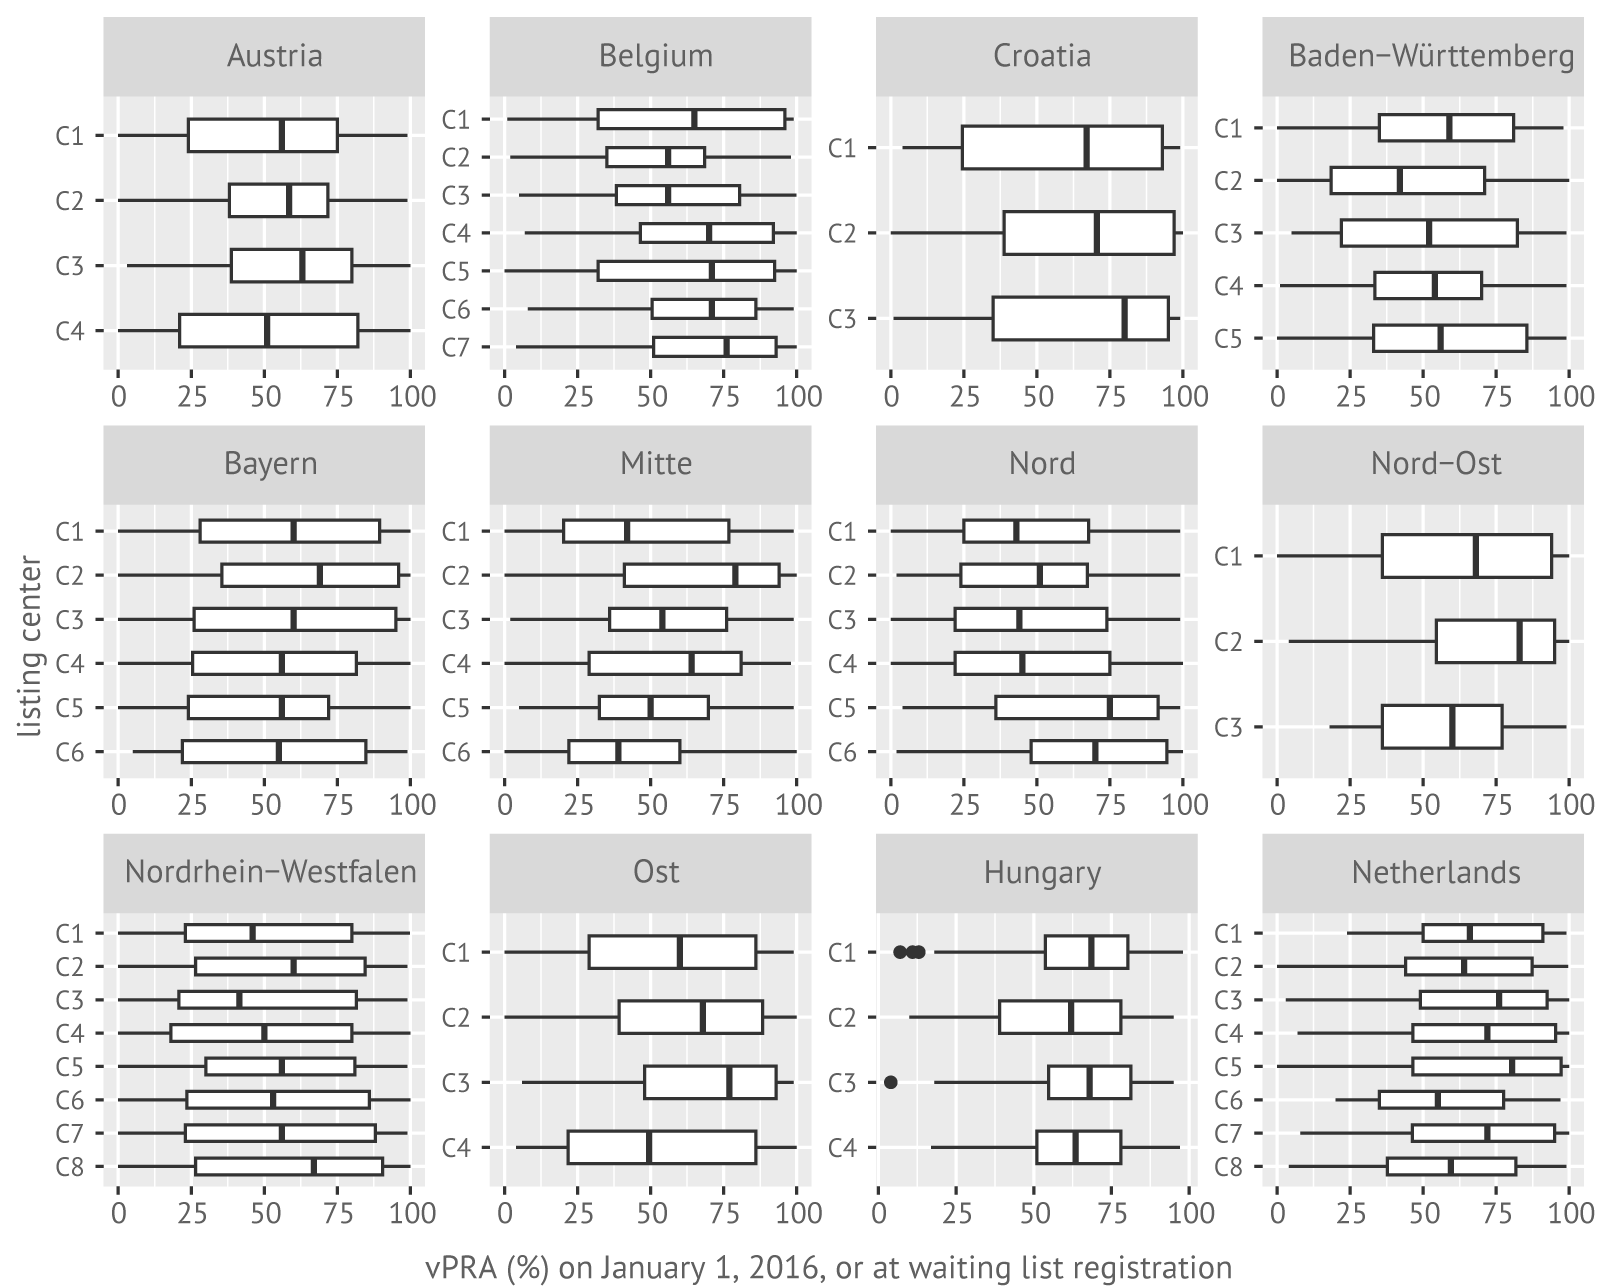
\includegraphics[width=1\linewidth]{figures/ch7//supp_figure_1} 

}

\caption{Distributions of the vPRA (\%) per center for immunized patients who were active on the kidney transplant waiting list between January 1, 2016, and January 1, 2020.}\label{fig:ch7sfig1}
\end{figure}

\FloatBarrier

\subsection{The association of the vPRA with ETKAS transplant rates}\label{the-association-of-the-vpra-with-etkas-transplant-rates}

The curve in Figure \ref{fig:ch7fig1} shows the estimated relation between
the relative transplant rate and the vPRA. The relative transplant rate
decreases with a higher vPRA. Adjusting for vPRA categories rather than
with a spline term yields similar results (horizontal dotted lines,
Figure \ref{fig:ch7fig1}). The relative transplant rate for patients with vPRA
0.1-50\% is estimated to be 23\% lower than non-immunized patients, and
51\% lower for patients with vPRA 75--85\%. For vPRAs exceeding 85\%, the
relative transplant rate decreases rapidly: it is 65\% lower for candidates
with vPRA ranging between 85\% and 95\% than for non-immunized candidates, and 94\%
lower for candidates with vPRAs ranging between 99 and 100\%.

\begin{figure}[ht]

{\centering 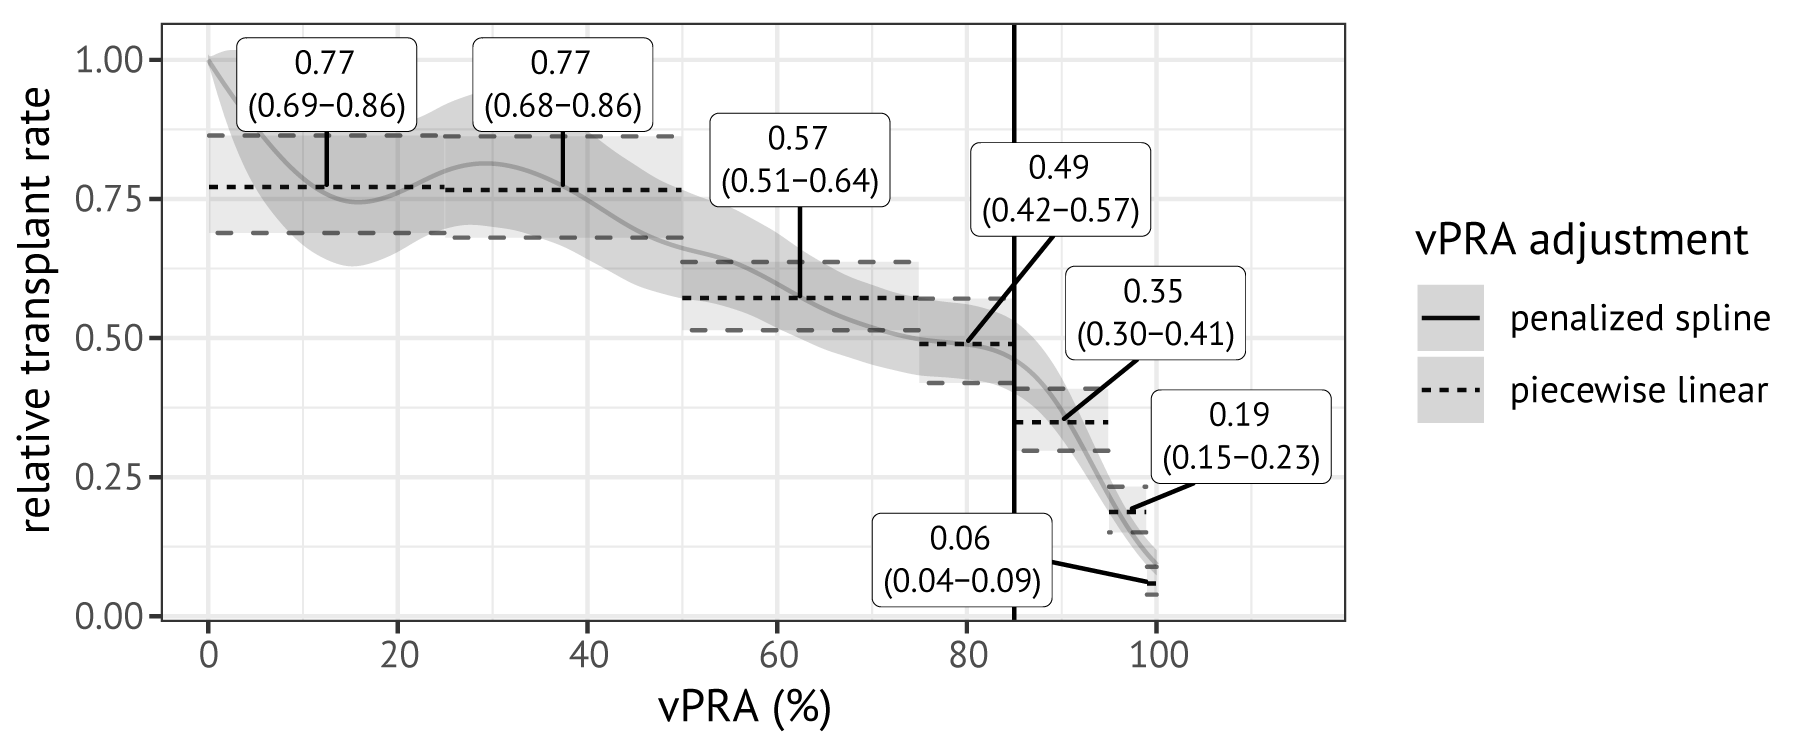
\includegraphics[width=1\linewidth]{figures/ch7//figure1} 

}

\caption{Relation between the relative ETKAS transplant rate and vPRA. This relation was estimated with a Cox proportional hazards model using vPRA as a time-varying variable and adjustment for other variables. The solid grey line was estimated using penalized spline terms with 8 degrees of freedom; the dotted lines were obtained by adjusting for discretized vPRA. Labels indicate point estimates of the hazard ratios for vPRA categories with 95\% confidence intervals.}\label{fig:ch7fig1}
\end{figure}

\subsection{Predicted transplant probabilities for a synthetic patient across Eurotransplant regions and blood groups}\label{predicted-transplant-probabilities-for-a-synthetic-patient-across-eurotransplant-regions-and-blood-groups}

Figure \ref{fig:ch7fig2} shows predicted transplant probabilities for a hypothetical
patient based on a Cox proportional hazards model fitted with delayed entry. This
hypothetical patient was defined as a patient who is a 49-year-old, male primary
transplant candidate, who had accrued 2 years of dialysis time at listing
and who remained transplantable and non-immunized (vPRA 0\%) during their waiting
list registration. The predicted probability of transplantation is almost 100\% within the first 4
years of registration in all Eurotransplant countries except for Germany where the
predicted probability of transplantation is just over 25\% (except for blood
group AB). Comparing transplant probabilities across blood groups shows that
blood group AB patients have the highest transplant rates in Austria, Hungary, and Germany,
but not in the Netherlands and Belgium. This suggests that a proportional
hazards assumption is implausible for blood group and highlights the
need for stratifying Cox models by both blood group and recipient
location.

\begin{figure}[ht]

{\centering 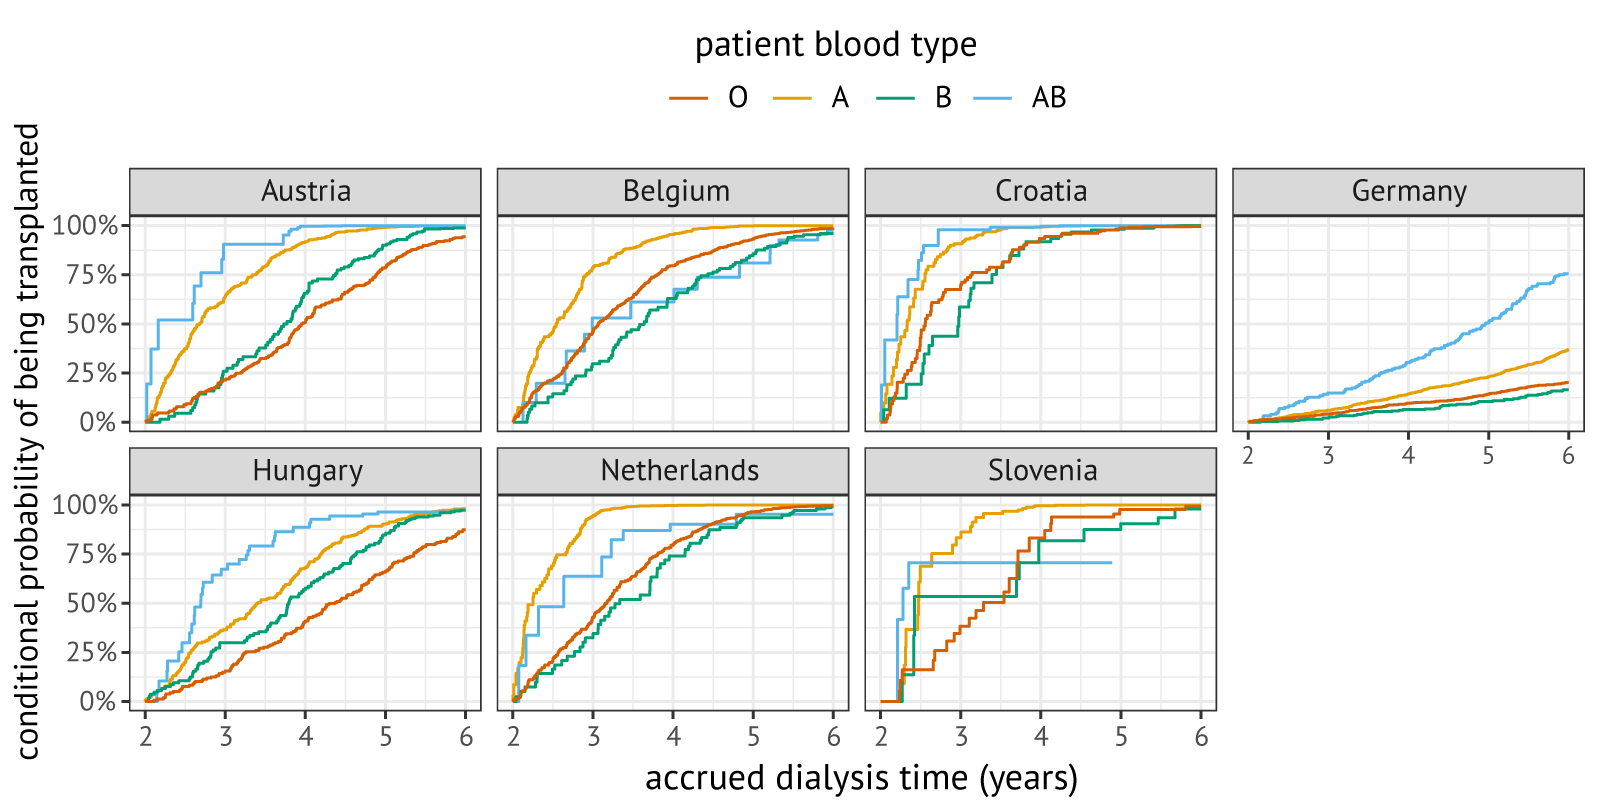
\includegraphics[width=1\linewidth]{figures/ch7//figure2} 

}

\caption{Predicted conditional probabilities of being transplanted within four years 
  upon entering the waiting list with two years of dialysis time, stratified by blood group
  and listing country. Predictions were made for a 49-year-old, male candidate who was listed for their first kidney transplantation. For Germany, distributions are displayed per DSO region.}\label{fig:ch7fig2}
\end{figure}

\subsection{Sensitivity checks for the main result}\label{sensitivity-checks-for-the-main-result}

Our main result is that a candidate's relative transplant rate decreases
substantially with an increasing vPRA, and that this decrease accelerates for
a vPRA exceeding 85\%. Figure \ref{fig:ch7fig3} shows sensitivity checks for this result.
For panel A models were re-estimated separately for German and non-German patients.
The inverse relation between the vPRA and relative transplant rate
is reproduced in both regions. An apparent difference between Germany and the
other Eurotransplant member countries is that the relative
transplant rates only appears to decrease for vPRAs greater than 50\% for German candidates,
while a decrease is visible over the whole domain for Eurotransplant's other member countries.
In panel B, we re-estimated models
separately in patients registered before and after January 1, 2016, the study start
state. This sensitivity check was motivated by the fact that
candidates already on the waiting list on January 1, 2016 are a
non-representative selection
of the kidney transplant candidate population. The estimated spline curves
are again very similar. In panel C, we assessed the impact of not using vPRA
as a time-varying variable. The obtained curves differ minimally, although it appears that
using time-fixed versions of the vPRA modestly increases effect
sizes. Finally, in panel D we assessed sensitivity of our result to the
availability of 0 DR-mismatched donors in Eurotransplant's donor pool. Also
here, no meaningful differences are found.

\begin{figure}[ht]

{\centering 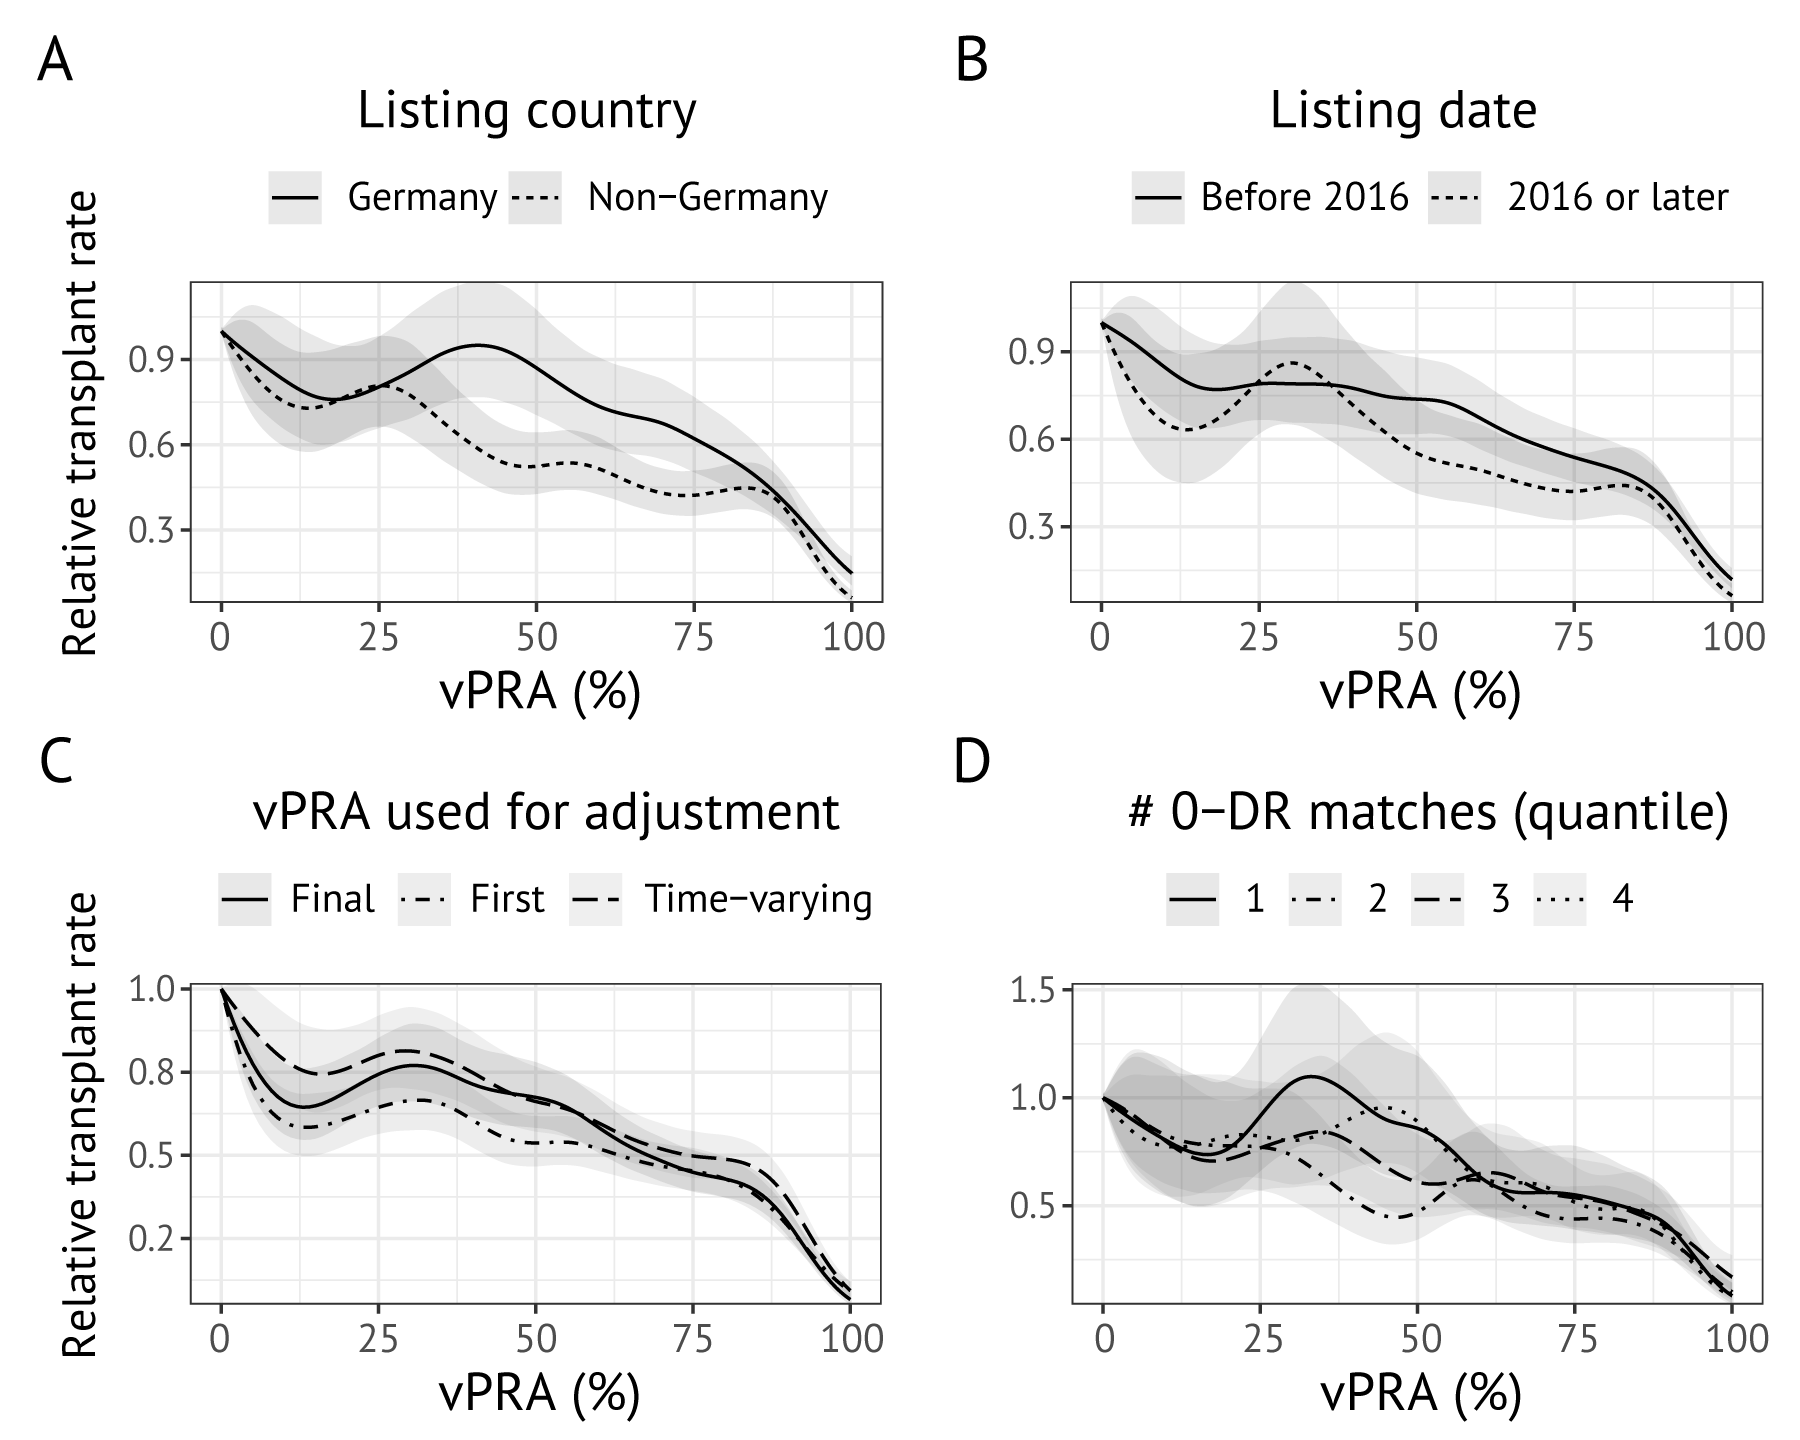
\includegraphics[width=0.99\linewidth]{figures/ch7//figure3} 

}

\caption{Sensitivity checks for the relation between the vPRA and relative transplant rate. Panel (a) shows penalized spline terms estimated separately for German allocation regions and Eurotransplant countries. Panel (b) shows penalized spline terms estimated separately for patients already on the waiting list on January 1, 2016, versus those registered afterwards. Panel (c) assesses whether the spline term is affected by whether a time-varying vPRA is used. Panel (d) shows how the relation between the relative transplant rate and vPRA varies by quantiles of the number of 0 DR-matchable donors. Panels (a), (b), and (d) use vPRA as a time-varying variable.}\label{fig:ch7fig3}
\end{figure}

\vfill

\newpage

\subsection{The association of the vPRA with ETKAS offer rates}\label{the-association-of-the-vpra-with-etkas-offer-rates}

The hazard ratios estimated for time-to-any-offer and time-to-high-quality-offer are
shown in Table \ref{tab:ch7tab2}. The hazard ratios obtained for the time-to-any-offer
analysis (first
row, Table \ref{tab:ch7tab2}) differed minimally from the hazard ratios obtained for the
relative transplant rate, at 28\% lower for vPRAs 50-75\%, 61\% lower
for vPRA 75--85\%, and a strong decrease for vPRA \textgreater85\%. When using a high-quality
offer as an outcome the inverse relation also reproduces (second
row), although estimated hazard ratios are attenuated. For example,
patients with a vPRA between 75 and 85\% have an approximate 33\% lower high-quality
offer rate than their non-immunized peers, while they have a 51\% lower transplant
rate and a 61\% lower any-offer rate.

\begin{table}[!h] \centering \caption{\label{tab:ch7tab2}Hazard ratios estimated in the time-to-offer analyses. The hazard ratios were estimated with a Cox proportional hazards model that uses vPRA as a time-varying variable and adjusts for other variables.} \centering \resizebox{\ifdim\width>\linewidth\linewidth\else\width\fi}{!}{ \begin{tabular}[t]{llllllll} \toprule \multicolumn{1}{c}{ } & \multicolumn{7}{c}{by vPRA} \\ \cmidrule(l{3pt}r{3pt}){2-8} offer & 0.01-24.9\% & 25-49.9\% & 50-74.9\% & 75-84.9\% & 85-94.9\% & 95-98.9\% & 99-100\%\\ \midrule any offer & \makecell{0.93\\(0.85-1.01)} & \makecell{0.72\\(0.66-0.79)} & \makecell{0.56\\(0.51-0.6)} & \makecell{0.39\\(0.35-0.44)} & \makecell{0.27\\(0.24-0.31)} & \makecell{0.16\\(0.14-0.19)} & \makecell{0.06\\(0.05-0.08)}\\ \cmidrule{1-8} high-quality offer & \makecell{0.88\\(0.77-1.02)} & \makecell{0.90\\(0.78-1.03)} & \makecell{0.72\\(0.63-0.81)} & \makecell{0.67\\(0.56-0.8)} & \makecell{0.51\\(0.43-0.62)} & \makecell{0.46\\(0.37-0.57)} & \makecell{0.20\\(0.15-0.29)}\\ \bottomrule \end{tabular}} \end{table}

\FloatBarrier

\subsection{Mismatch probability points awarded for the vPRA}\label{mismatch-probability-points-awarded-for-the-vpra}

Immunized patients are indirectly awarded points in ETKAS through points awarded
for the mismatch probability (MMP), which is a quantification of the frequency of favorably
matched donors. Candidates with rare
blood groups or difficult-to-match HLAs may receive very few extra points for being
sensitized, as the MMP is by definition higher for candidates with rare blood groups or those with difficult-to-match HLA phenotypes. To highlight this, we calculated for
all immunized patients the difference between mismatch probability
points calculated based on their actual vPRA, and mismatch probability
points with a vPRA of 0\%. This difference is the number of mismatch probability
points that the candidate received on the basis of their vPRA.
\newpage
Figure \ref{fig:ch7fig4} shows the distributions of MMP points that the immunized patients in our cohort received based on
the vPRA. Immunization indeed results only in a marginal increase in the number
of points received for candidates with rare blood groups: the median
sensitized candidate with blood group AB receives fewer than 20 additional
MMP points, regardless of their vPRA. Moreover, a quarter of patients with
the highest vPRAs (\textgreater85\%) receive less than 50 mismatch probability points
based on their vPRA. The number of additional MMP points awarded based
on the vPRA thus appears meagre compared to the median number of ETKAS points needed for
transplant through ETKAS, which exceeded 900 points between
January 1, 2016, and January 1tab1, 2020.

\begin{figure}[ht]

{\centering 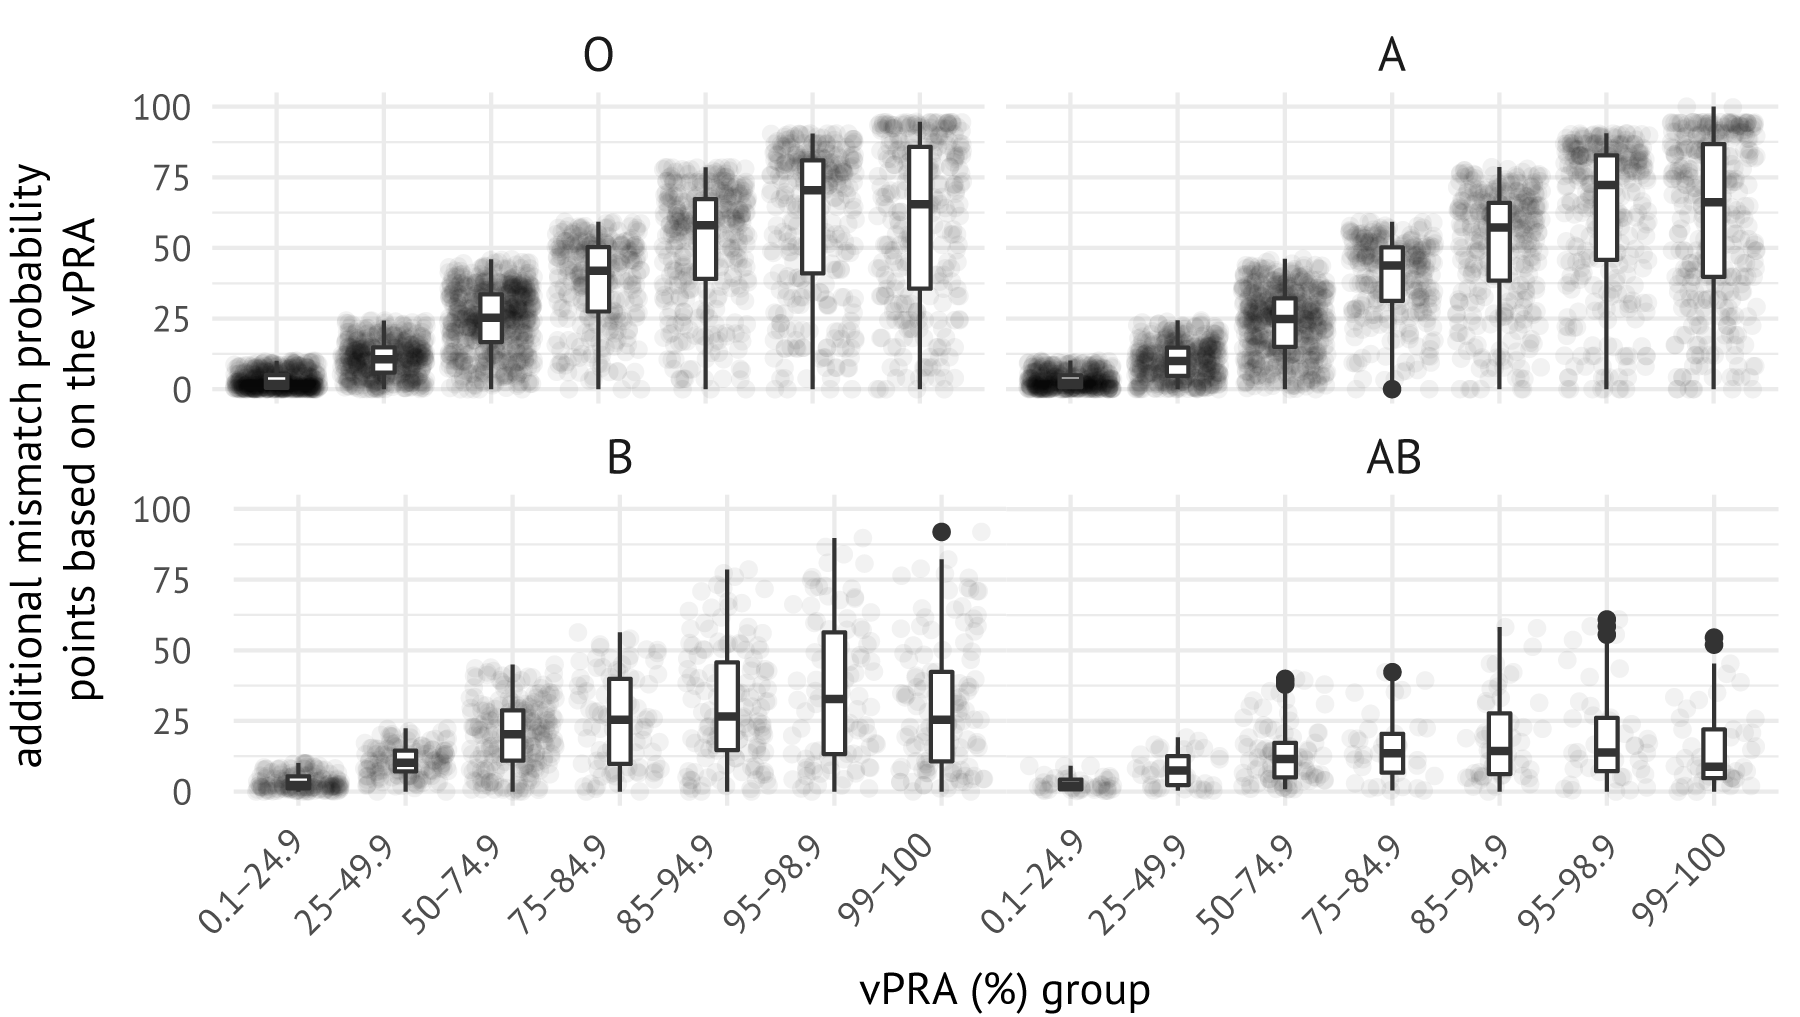
\includegraphics[width=0.95\linewidth]{figures/ch7//figure4} 

}

\caption{Mismatch probability points awarded to immunized patients based on their vPRA. Each dot represents an immunized patient in the cohort. Statistics were obtained by calculating the difference in MMP calculated with the actual vPRA versus the MMP calculated with a vPRA of 0\%.}\label{fig:ch7fig4}
\end{figure}

\FloatBarrier

\section{Discussion}\label{discussion-2}

More than 90\% of immunized kidney transplant candidates in Eurotransplant
rely on ETKAS for access to kidney transplantation. Concerns exist that these candidates
are inadequately served by the mismatch probability points, and that they face extended
waiting times \citep{susal2015, ziemannUnacceptableHumanLeucocyte2017, zecherImpactSensitizationWaiting2022a}.
This motivated us to study the relation between the vPRA and relative
transplant rate in ETKAS. Our study is the first to quantify this relation
Eurotransplant-wide, and complements two previous studies that used German
cohorts \citep{ziemannUnacceptableHumanLeucocyte2017, zecherImpactSensitizationWaiting2022a},
\newpage
We studied the relation with Cox regression stratified by blood group
and recipient country, using accrued dialysis time as the timescale.
In this analysis, we allowed for delayed entry and included the vPRA as a
time-varying variable. This study design avoids some methodological issues of the
previous studies. Dialysis time is a more appropriate timescale than
Ziemann et al.'s time-since-listing, as ETKAS allocation prioritizes
based on accrued dialysis time and not waiting time. Zecher et al.~used
total accrued dialysis time as the outcome, and associated this with the vPRA recorded
on January 1, 2019, which was their study start date. This appears problematic as over half of the
immunized patients change the set of unacceptable antigens during
registration, which means that the vPRA recorded on January 1, 2019 is not
pre-determined to their accrued dialysis time. Our analyses avoided this issue
by allowing for delayed entry of transplant candidates (not modeling
transplant rates before January 1, 2016) and using the vPRA as a time-varying
variable.

Our results show that a higher vPRA is associated with significantly reduced
relative transplant rates in ETKAS. Unlike prior studies, reductions in
transplant rates are already highly significant for vPRAs below
85\%, with transplant rates 23\% lower for vPRAs from 0--50\%
(p \textless{} 0.001) and 51\% lower for vPRAs 75--85\% (p \textless{} 0.001). Transplant rates
are even lower for candidates with vPRA exceeding 85\%; for example, candidates with
vPRAs greater than 99\% face 94\% lower transplant rates. We note that candidates with
vPRAs exceeding 85\% may still depend on access to transplantation through ETKAS, for
example because their center does not participate in the AM program or because
the candidate does not meet AM criteria (unacceptable antigens require
CDC reactivity or documentation of a sensitizing event \citep{Heidt2021}).
One possible reason why even candidates with very low vPRAs (0-10\%) face
reduced access to transplantation is that immunized candidates
could not be selected in non-standard allocation in the study period, which
accounts for approximately 10\% of kidney transplantations in Eurotransplant.

A strength of our study is the inclusion of several sensitivity checks, which show that the inverse
relation between vPRA and the transplant rate generalizes beyond Germany,
is independent of whether the patient was listed before or after 2016, and is
independent of the type of vPRA used (time-varying, first vPRA, or final vPRA).
The difficulty of finding a high-quality match (defined as the number of donors
with 0 HLA-DR matches) also does not affect the relation.

A limitation to our study is that attention was restricted to patients
eligible for ETKAS only, with patients censored if they enrolled into the
AM program or became eligible for ESP. Zecher et al.~instead adjusted in
their analyses for enrolment in the AM program. We did not pursue this, as
AM allocation is not based on accrued dialysis time which makes the proportional
hazards assumption implausible. Ziemann et al.~and Zecher et al.~both also
studied time-to-transplant for ESP patients. We did not pursue this, as candidates can choose to continue their participation in ETKAS after their 65th birthday, and it is not clear how to correct for the resulting selection bias. Moreover, elderly patients listed
in other Eurotransplant member countries can simultaneously participate in ETKAS
and ESP, and it is unclear how to appropriately account for the simultaneous
participation of candidates in these in our analysis. Another limitation to our
study is that sensitization against
HLA-DQA, -DPA and -DPB may further limit transplant rates due to positive
physical cross-matches. These antibody specificities were not captured by
the vPRA used in this analysis.

Our secondary analyses showed that the vPRA is also inversely related to
ETKAS kidney offer rates, both when considering any offer as an outcome
and when considering only high-quality offers as an outcome. This
suggests that the reduced transplant rate for immunized patients is
a result of ETKAS allocation, and not the kidney offer acceptance behavior of
the transplant centers. We showed that many immunized patients receive only a marginal amount of
additional MMP points based on their vPRA, in particular those with a difficult-to-match
HLA or rare blood group. A potential policy implication of our work is thus
that it seems worthwhile to revise the number of points that is awarded for the MMP,
which has remained capped at 100 points since the introduction of ETKAS
in 1996.

Finally, our work can help inform decision-making on whether to assign
non-CDC reactive antigens as unacceptable. For ETKAS such decisions are
made based on personalized risk assessments by doctors and local HLA
laboratories, not on criteria prescribed by Eurotransplant. Our finding
that increases in the vPRA beyond 85\% strongly
decreases the transplant rate may, for example, motivate local
transplant professionals to be cautious in assigning antigens without
CDC-reactivity as unacceptable for patients with already high vPRA
(\textgreater85\%). In this way, our work could help avoid situations where caution
of local transplant teams unintentionally prolongs a candidate's waiting time.

\chapter{The ETKidney simulator}\label{CHetkidneysimulator}

\chaptermark{The ETKidney simulator}

\vfill

\begin{center}\rule{0.5\linewidth}{0.5pt}\end{center}

\noindent
An article based on this chapter has been submitted for publication:
de Ferrante, H.C., Laguna-Goya, R., Smeulders, B.M.L., Spieksma, F.C.R., Tieken, I.

\newpage
\normalsize

\subsubsection*{Abstract}

A barrier to modernizing ETKAS and ESP kidney allocation
rules is that Eurotransplant lacks tools to quantitatively assess the
impact of kidney allocation policy changes. We present the ETKidney simulator,
which was developed for this purpose. This tool simulates kidney allocation
according to the actual ETKAS and ESP allocation rules. The ETKidney simulator was
developed in close collaboration with medical doctors from
Eurotransplant, and was presented to the Eurotransplant Kidney
Advisory Committee as well as other major
stakeholders. To enhance trust in the tool, the ETKidney simulator
has been made publicly available together with synthetic data.

In this chapter, we describe the ETKidney simulator in detail and validate
the simulator by comparing simulated outcomes to actual ETKAS and ESP
outcomes between April 1, 2021, and December 31, 2024. We illustrate
how the simulator can contribute to the evaluation of alternative kidney allocation
policies with three clinically motivated case studies. We anticipate
that the ETKidney simulator will be pivotal in modernizing ETKAS and
ESP allocation rules by enabling informed decision-making on kidney
allocation rules in collaboration with national competent authorities.

\newpage
\normalsize

\section{Introduction}\label{introduction-4}

Potential improvements to ETKAS and ESP are regularly proposed, and are
often based on medical insights or ethical considerations. For instance,
proposals have been made to emphasize DR matching in ETKAS
\citep{vereerstraetenAllocationCadaverKidneys1999, doxiadisSimplerEquitableAllocation2007},
motivated by findings that mismatches at the HLA-DR locus are most deleterious to graft
survival \citep{Roberts2004, johnsonFactorsInfluencingOutcome2010}.
Other proposals include making candidates under the age of 65 eligible for ESP
\citep{Ssal2020}, introducing HLA-DR matching in ESP \citep{deFijter2023}, introducing candidate-donor age matching
\citep{vonsamson-himmelstjernaContinuousDonorrecipientAge2024}, basing HLA matching on epitope
matching \citep{Niemann2021}, and giving extra priority to the candidates who
are immunized but do not qualify for the Acceptable Mismatch (AM) program
\citep{ziemannUnacceptableHumanLeucocyte2017, zecherImpactSensitizationWaiting2022a}.

Within Eurotransplant, such areas for improvement are regularly discussed
by the Eurotransplant Kidney Advisory Committee (ETKAC), whose members are
nephrologists who represent the Eurotransplant member countries,
an abdominal surgeon, and an immunologist. Despite regular ETKAC discussions
on the aforementioned topics, ETKAS and ESP have not changed much since their
initiations in 1996 and 1999, respectively. To support discussions within ETKAC
and discussions with national competent authorities, Eurotransplant requires a tool that can
quantify the impact of policy changes in ETKAS and ESP. Computer simulations
can be used for this purpose.

The use of computer simulations to design kidney allocation systems is not new.
In fact, ETKAS itself was based on computer simulations that were published in
in 1993 \citep{wujciakComputerAnalysisCadaver1993, wujciakProposalImprovedCadaver1993a}. Other organ allocation organizations also
routinely note the usage of computer simulations. For example, in the United States,
the Kidney-Pancreas Simulated Allocation Model (KPSAM) was used to revise allocation rules
in 2014 \citep{israniNewNationalAllocation2014}, and this tool continues to
be used for the proposal of further changes to allocation
\citep{israniNewKidneyPancreas2021, mankowskiAcceleratingKidneyAllocation2019}.
The kidney allocation policies in France and the United Kingdom were also
updated on the basis of bespoke computer simulations in 2015 and 2019,
respectively \citep{jacquelinetChangingKidneyAllocation2006, Audry2022, Mumford2018}.
A bespoke model for Eurotransplant has not been available.

This motivated us to develop a simulation toolbox that enables
Eurotransplant and other stakeholders to quantify the impact of changes
to ETKAS and ESP allocation rules. This tool, which we refer to as the
ETKidney simulator, uses discrete-event simulation (DES) to mimic kidney
allocation within Eurotransplant. The simulator was developed in close
collaboration with medical doctors from Eurotransplant and was presented
on several occasions to ETKAC, which has welcomed the ETKidney simulator as a tool to
inform policy discussions on kidney allocation. The Python code of the
simulator is made publicly available together with synthetic data to
enable collaborations with policymakers and scientists in evaluating
alternative ETKAS and ESP allocation rules.\footnote{\url{https://github.com/hansdeferrante/Eurotransplant_ETKidney_simulator}}

\newpage

In this chapter, we
describe how kidneys are allocated within Eurotransplant (Section \ref{sec:etkidneyalloc}) and how this process is approximated by
the simulator (Sections \ref{sec:etkidneydesign} and \ref{sec:etkidneymodules}). We also give insight into how closely
the simulator approximates outcomes of ETKAS and ESP with input-output
validation (Section \ref{sec:etkidneyvv}), and demonstrate how the ETKidney
simulator can contribute to policy evaluation with three clinically relevant
case studies (Section \ref{sec:etkidneycasestudies}).

\section{The kidney allocation programs of Eurotransplant}\label{sec:etkidneyalloc}

Figure \ref{fig:ch8fig1} shows how Eurotransplant
allocates the deceased-donor kidneys that become available for
kidney-only transplantation.\footnote{In case a multi-organ donor is reported to Eurotransplant,
  the donor's kidneys may first be accepted by candidates waiting for a combined
  transplantation of a kidney with another organ (heart, lung, pancreas, liver, or intestine).
  These combined transplantations account for 7\% of all deceased-donor kidney transplants
  in Eurotransplant \citep{statlibrary2152P_AllET_Kidney}.} Three standard allocation programs are
used to place these kidneys: the AM program, ETKAS and ESP (see Figure \ref{fig:ch8fig1}).
The program through which Eurotransplant offers the kidney(s) is determined by
the age of the donor. Kidneys from donors under the age of 65 are first offered for
transplantation through the AM program, which accounted for 3\% of
kidney-only transplantations between 2014 and 2023, and then through
ETKAS, which accounted for 69\% of kidney-only transplantations. The ESP is
used to allocate kidneys from donors aged 65 or older, and accounted for
16\% of kidney-only transplantations \citep{etStatsLibrary2072P}.

\begin{figure}[h]

{\centering 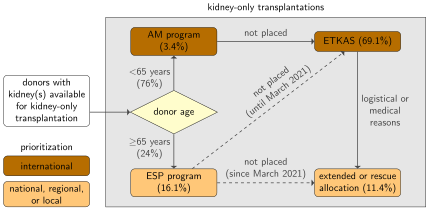
\includegraphics[width=0.96\linewidth]{figures/ch8//fig1-flowchart_kidney_allocation} 

}

\caption{Flow chart illustrating how Eurotransplant offers kidneys for kidney-only transplantation. The percentages shown represent the proportion of kidney-only transplantations performed through each mechanism between 2014 and 2023. Kidneys declined by all candidates in ESP were re-allocated via ETKAS until March 2021. Since March 2021, such kidneys are instead offered via extended ESP allocation, in which non-local candidates and those aged below 65 can participate since March 2021.}\label{fig:ch8fig1}
\end{figure}

The remaining 11\% of kidney-only transplantations between 2014 and 2023
resulted from \emph{non-standard allocation}, which Eurotransplant can initiate
if the loss of a transplantable graft is anticipated. In non-standard allocation,
Eurotransplant offers the grafts to centers in the vicinity of the kidney(s),
either through extended or rescue allocation. In extended kidney allocation, centers
have 60 minutes to propose candidates. In rescue allocation, offers are competitive,
which means that the first center to respond receives the kidney. Not all kidneys offered by
Eurotransplant are eventually transplanted.
In fact, approximately 24\% of the kidneys that were offered by Eurotransplant
for transplantation between 2014 and 2023 were discarded \citep{etreport_1132P}.

Match lists determine which candidate receives an offer at
what moment. The composition and ordering of
candidates on match lists are determined by program-specific
\emph{eligibility}, \emph{filtering}, and \emph{ranking criteria}. The eligibility
criteria determine whether a candidate is allowed to appear on the match list
under Eurotransplant kidney allocation rules. Examples of eligibility criteria are that the
candidate must have the same blood group as the donor, and that the donor's HLA
must not include an HLA antigen that the center has reported as unacceptable for
the candidate.
\newpage
The filtering criteria also determine whether Eurotransplant contacts
the center to make an offer for a specific candidate. While eligibility criteria
are rules imposed by Eurotransplant, filtering criteria represent the preferences
that transplant centers have on kidney offers.
The filtering criteria can be distinguished into:

\begin{enumerate}
\def\labelenumi{\arabic{enumi}.}
\tightlist
\item
  \emph{allocation profiles}, with which centers can indicate that their
  patient does not want to receive offers from donors with certain
  characteristics (e.g.~donors above a certain age, donors with a specific
  virology, or other donor-related characteristics), and
\item
  \emph{HLA mismatch criteria}, with which centers can specify their minimum
  requirements for the HLA match quality between the donor and
  candidate on the HLA-A, -B, and -DR loci.
\end{enumerate}

Finally, the ranking criteria determine the position of a candidate on the
match list. An overview of the ETKAS- and ESP-specific ranking criteria is included
in Section \ref{sec:etkidneympmod}.

In standard allocation, Eurotransplant only offers kidneys to candidates
who appear on the \emph{filtered match list}, which means that candidates must
meet the program's eligibility and filtering criteria. In extended allocation,
centers are allowed to select candidates from the \emph{unfiltered match list},
which means that candidates only have to meet the program's eligibility criteria.
In rescue allocation, centers can also propose other candidates
for transplantation, including those with
non-identical ABO blood groups.

\section{Purpose and design of the ETKidney Simulator}\label{sec:etkidneydesign}

We use discrete-event simulation (DES) to simulate kidney allocation according to the
actual ETKAS and ESP allocation rules implemented in March 2021. Simulation of
the AM program is beyond the scope of the ETKidney simulator, because
the definition of acceptable antigens is based on an individualized
risk-benefit analysis which requires specialized immunological
knowledge. We note that the simulator has not been designed for the analysis of
kidney discard rates.

Relevant states for the simulation are (i) the statuses of candidates on the ETKAS or ESP
waiting lists, (ii) the export
balances of Eurotransplant member countries, which affect a candidate's
rank on ETKAS match lists because of Eurotransplant's balance point
system (see Section \ref{sec:etkidneybalance}). In DES, we study how these system states
evolve in response to a series of discrete events. For the ETKidney
simulator, we distinguish between three types of events, which are:

\begin{enumerate}
\def\labelenumi{\arabic{enumi}.}
\item
  \emph{candidate status updates}; these include changes to a candidate's waiting
  list status (transplantable, non-transplantable, HU, removed, transplanted,
  or deceased), their allocation profiles, their unacceptable antigens,
  their HLA mismatch criteria, the reporting of an antibody screening,
  or a choice between ETKAS or ESP in Germany (where these programs are mutually exclusive),
\item
  \emph{donor arrivals}; these are donors reported to Eurotransplant for whom one or two kidneys become available for kidney-only transplantation through ETKAS or ESP, which generally
  results in a transplantation, and
\item
  \emph{balance update events}; these are transplantations across country borders
  through allocation programs other than ETKAS and ESP. These transplantations
  also count towards the export balances of Eurotransplant's member countries, based
  on which balance points are awarded.
\end{enumerate}

\subsection{Input data for the ETKidney simulator}\label{sec:etkidneyinputstreams}

Users of the ETKidney simulator have to specify the input streams that
define the candidate status updates and donor arrival events. Furthermore, an input stream of
international transplantations can be specified, which is used to
initialize ETKAS balances and to define balance update events. For candidates
and donors, the data in the input streams must include
all administrative and medical information required by the eligibility,
filtering, and ranking criteria. Additional information may be required
by the graft offer acceptance module to simulate the decision-making of kidney
transplant centers in accepting kidney offers, and by the post-transplant module to simulate post-transplant
survival.

For candidates, the input streams must include complete information on
what would happen to each candidate until they exit the waiting list,
either because of a waiting list removal or a waiting list death. This requirement
implies that candidate input streams cannot
be solely based on historical registry data: after all, waiting list
removals or waiting list deaths have not been observed for candidates who were
transplanted via ETKAS or ESP.

For simulations done in this chapter, we use input streams based on
historical data. The actual status update trajectories of candidates are complemented
with statuses copied over from comparable candidates who remained registered
on the waiting list. For this, we use a procedure to complete a candidate's
status updates that was originally developed for the ELAS simulator (see Chapter \ref{CHelassimulator} and Appendix \ref{APPimputation}).

\subsection{Initialization of the ETKidney simulator's system state}\label{sec:etkidneyinit}

The balance system is initialized using data from the input stream for international transplantations:
all international transplantations that were performed prior to the simulation
start date are processed, which ensures that the balances are correctly initialized.
Additionally, the
simulator schedules a balance update event for every cross-border transplantation
that occurs within the simulation window via combined transplantations or via the AM
program. This is necessary to accurately simulate the evolution of balances,
because such transplantations also count towards a member country's export balance.

From candidate input streams, the simulator loads all candidates who
have an active status on the waiting list within the simulation window.
The listings of candidates listed for repeat kidney transplantation whose initial
transplantation takes place within the simulation window are excluded, which
is necessary to ensure that a candidate cannot simultaneously wait for a
primary and repeat transplantation in ETKidney simulation runs. For each candidate,
a single patient event is scheduled in the Future Event Set (FES) timed at the
candidate's first available status update. The scheduling of subsequent status
updates is postponed until the status update has been processed.

From donor input streams, all donors reported during the simulation
window are loaded. For each donor, a donor event is scheduled in the FES
on the donor reporting date.

\newpage

\subsection{Overview of the simulation}\label{sec:etkidneyoverview}

Figure \ref{fig:ch8fig2} illustrates how events are processed in the simulation.
The balance update events are handled by simply updating the export balances
of the countries that were involved in the international transplantation. The
patient events are handled by updating the status
of the corresponding patient. Handling of donor events is more complex, because
the allocation of the kidney(s) through ETKAS or ESP has to be approximated
by the simulator.

\begin{figure}[ht]

{\centering 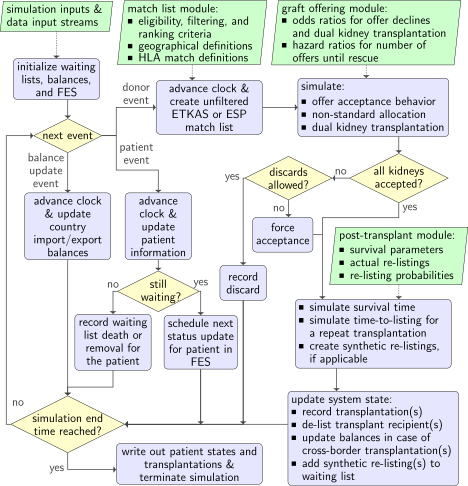
\includegraphics[width=0.9\linewidth]{figures/ch8//fig2-event_handling_flowchart} 

}

\caption{Event handling flowchart for the ETKidney simulator. Inputs and parameters are represented using parallelograms. If a kidney is declined by all candidates, simulation settings determine whether a discard is recorded or a candidate is forced to accept the kidney for transplantation. FES, Future Event Set.}\label{fig:ch8fig2}
\end{figure}

\newpage
To approximate such kidney-only allocation, the ETKidney simulator's
\emph{match list module} was developed (see Section
\ref{sec:etkidneympmod}). This module first
creates, depending on the age of the donor, an unfiltered ETKAS or ESP
match list that contains for each candidate who meets the
corresponding program's eligibility criteria a \emph{match record}. These match records
are automatically ordered based on the respective
program's ranking criteria, with the number of points awarded to each
match record determined by the \emph{point score module} (see Section
\ref{sec:etkidneympmod}).

Using the ordered match list as the input, the \emph{graft offering} module simulates
which candidates accept the kidneys (see Section
\ref{sec:etkidneyacceptance}). In rare cases, all candidates on the match list
are simulated to decline the kidney offer. If this
happens for an ESP match list, the graft offering module will
try to place the kidneys through non-standard ESP allocation, which is
how Eurotransplant allocates kidneys from donors aged 65 or older since
March 2021. In the rare event that kidneys remain unplaced, the graft offering module
can either (i) record a discard for the kidney(s), or (ii) force transplantation of the
candidate who was predicted to be most likely to accept the graft.
For the simulations in this chapter, option (ii) is used because
the donor input stream used for simulation consists only of donors whose
kidneys were actually transplanted through ETKAS and ESP.

After a graft has been accepted, transplantations are recorded with the
kidney balances updated in case of a cross-border transplantation.
The \emph{post-transplant module} simulates post-transplant outcomes for transplant
recipients. In case a candidate is simulated to enlist for repeat transplantation,
this module also schedules a \emph{synthetic re-listing} (see Section
\ref{sec:etkidneysynthreg}).

\section{Modules of the ETKidney simulator}\label{sec:etkidneymodules}

This section describes key modules of the ETKidney simulator: the HLA
system module (Section \ref{sec:etkidneyhla}), the balance system module
(Section \ref{sec:etkidneybalance}), the match list and point system
module (Section \ref{sec:etkidneympmod}), the graft offering
module (Section \ref{sec:etkidneyacceptance}), and the post-transplant module
(Section \ref{sec:etkidneyposttxp}).

\subsection{The HLA system module}\label{sec:etkidneyhla}

The HLA system module implements all mechanisms through which
Eurotransplant prioritizes HLA matching. These procedures are (i)
determining how many mismatches there are at the HLA loci of interest, (ii)
calculating the vPRA on the basis of unacceptable antigens, and (iii)
calculating the mismatch probability.

\subsubsection{Calculation of HLA mismatches}\label{sec:etkidneyhlammcalc}

The HLA system module can determine, for a given patient HLA and given
donor HLA, how many antigen mismatches there are per locus (0, 1, or 2).
The simulation settings file specifies at which HLA loci mismatches are to
be determined. By default, the module only counts mismatches
at the HLA-A, -B, and -DR loci, because the current ETKAS point
system only awards points for these mismatches. HLA-A and HLA-B
mismatches are determined at the level of broad antigens, while HLA-DR
mismatches are determined at the level of split antigens (as is done
for allocation in ETKAS, see \citep{manualKidney}).

\subsubsection{Quantification of virtual Panel-Reactive Antibodies (vPRA)}\label{sec:etkidneyvpracalc}

A candidate's vPRA affects a candidate's position on the match list
because the vPRA is used to calculate the mismatch probability.
In simulations included in this chapter the vPRA is quantified by
counting the fraction of donors that carry unacceptable antigens in
the ETRL donor panel (V4.0). This database includes the HLA phenotypes
of 10,000 donors that were recently reported to Eurotransplant.
The HLA system module can also quantify the
vPRA against a user-specified input database of 10,000 donor HLAs.

\subsubsection{Calculation of the Eurotransplant mismatch probability (MMP)}\label{sec:etkidneymmp}

ETKAS awards points for the mismatch probability, which is the chance
that there is \emph{no} favorably matched donor for a candidate among the next
1,000 donors reported to Eurotransplant. Eurotransplant calculates
this mismatch probability analytically as:
\[\texttt{MMP} = \Bigl(1 - f_{BG}\cdot (1-\texttt{vPRA})\cdot p_{\leq1mm}\Bigr)^{1000},\]
where \(f_{BG}\) is the candidate's blood group frequency and
\(p_{\leq1mm}\) is a quantification of the probability that a donor has at
most 1 HLA-ABDR mismatch with the candidate.

By default, \(p_{\leq1mm}\) is calculated with analytic formulas for the probability of
receiving exactly 0 mismatches and exactly 1 mismatch, which are also used for ETKAS
allocation. A disadvantage of this approach is that both these formulas assume
that HLA antigens are independently distributed according to their population
frequencies, which ignores HLA linkage disequilibrium. To resolve this, the
HLA system module can also quantify the availability of favorably matched donors
by counting the number of 0- or 1-ABDR mismatched donors among the pool of 10,000
donors used to calculate the vPRA, which we denote by \(f_{\leq1mm}\). Using this
quantity, we define the \emph{``1-ABDR HLA mismatch frequency''} as
\[\Bigl(1- f_{\leq1mm}\Bigr)^{1000}.\] We note that this quantity does not
take into account the candidate's blood group, nor the candidate's vPRA.
We use this quantity in the second case study (see Section
\ref{sec:etkidneycasestudyvpra}).

\subsection{The balance system module}\label{sec:etkidneybalance}

To balance the international exchange of kidneys, Eurotransplant keeps track of
the \emph{net kidney export balances} of its member countries, and awards points in
ETKAS based on these balances.\footnote{The number of balance points awarded is calculated
  by subtracting from each member country's export balance the export balance of
  the country which is the largest importer (a negative number), and multiplying
  the outcome by the balance weight. This balance weight is currently 30.} Within Austria, an additional regional balance system
exists to ensure that the Austrian regions benefit equally from
cross-border transplantations \citep{manualKidney}. The balance system module
implements both these national and regional balance systems for the ETKidney
simulator. Initialization of the net export balances is possible, and can be based on
historical data. By default, separate balances are maintained for each donor
age group (0-17 years, 18-49 years, 50-64 years, or 65 years or older), which
is consistent with how balances have been maintained since April 1, 2019 \citep{manualKidney}.

\subsection{The match list module \& point system module}\label{sec:etkidneympmod}

The match list module is used to create ETKAS or ESP match lists, which
serve as input for the graft offering module. Only candidates who meet
the corresponding program's eligibility criteria appear on match lists,
with each candidate ranked based on \emph{tiers} and \emph{points}. Candidates
ranked in higher tiers receive priority over candidates in
lower tiers. Within each tier, candidates are ranked by points. In ETKAS,
tiers are in order of descending priority:

\begin{enumerate}
\def\labelenumi{\arabic{enumi}.}
\item
  candidates with zero HLA-ABDR mismatches with the donor,
\item
  pediatric candidates, in case the donor is also pediatric,
\item
  all other candidates.
\end{enumerate}

The ETKAS point system awards:

\begin{enumerate}
\def\labelenumi{\arabic{enumi}.}
\item
  33.33 points per year of accrued dialysis time,
\item
  400 minus 66.66 points per HLA-ABDR mismatch. These points are
  doubled if the candidate is pediatric,
\item
  100 points if the candidate is pediatric,
\item
  500 points if the candidate has the High Urgency (HU) status,
\item
  up to 100 mismatch probability points,
\item
  balance points, the amount of which is determined based on the net export balances of
  Eurotransplant's member countries,
\item
  up to 300 distance points if the candidate is located in the same
  country as the donor. The specific amount awarded depends on the
  country, see the kidney manual for an overview \citep{manualKidney}.
\end{enumerate}

Since March 2021, ESP allocation has been based on nine tiers, which are defined
based on the location of the candidate relative to the donor and whether the
candidate is 65 years or older. Within ESP tiers points are awarded
based on the dialysis time that a candidate has accrued \citep{manualKidney}.

\subsection{The graft offering module}\label{sec:etkidneyacceptance}

The graft offering module mimics how Eurotransplant offers kidneys to
centers for transplantation, and returns, based on a match list, the
candidates who accept the kidney for transplantation (if any). How kidney
offers are simulated in the ETKidney simulator is illustrated in Figure
\ref{fig:ch8fig3}. The module first simulates, based on the donor, the
maximum number of offers made in standard allocation. We denote this number by \(k\). The module then makes kidney offers to
candidates in order of their ranking on the \emph{filtered} match list,
either until \(k\) offers have been made or until all available kidneys
have been accepted for transplantation.

\begin{figure}[ht]

{\centering 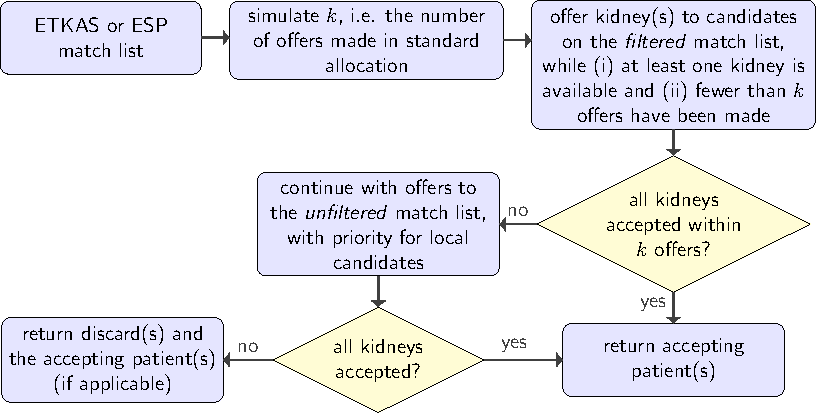
\includegraphics[width=0.9\linewidth]{figures/ch8//fig3-graft_offering_diagram} 

}

\caption{Flow chart summarizing how the ETKidney simulator approximates the graft offering process.}\label{fig:ch8fig3}
\end{figure}

If not all kidneys have been accepted after \(k\) offers in standard
allocation, the match lists are re-ordered with priority for
candidates located in the vicinity of the donor to
approximate non-standard allocation. At this point, the module also makes
offers to candidates who appear only on the \emph{unfiltered} match list,
as centers can select such candidates in extended and rescue allocation.
Offers in non-standard allocation are made either until all kidneys have been accepted
or until the match list is exhausted. The module then returns the candidates who have
accepted the kidneys.

\subsubsection{Simulating the switch to non-standard allocation}\label{sec:etkidneynonstandard}

The graft offering module switches to non-standard allocation following \(k\)
declines. We modeled \(K\) with a Cox proportional hazards model with
adjustment for donor characteristics (donor age, virology, death cause,
last creatinine, diabetes, smoking, proteinuria, blood group, and
extended donor criteria). Cox models were stratified by the program
(ETKAS / ESP), and within ETKAS additionally by the donor country.
The baseline hazards and parameters needed to simulate from this model
are made available with the ETKidney simulator. These were estimated
on match lists generated between January 1, 2014, and January 1, 2024. ESP match lists
from before March 2021 were excluded for estimation of these parameters,
because non-standard allocation was rarely used in ESP before March 2021.\footnote{
  Before March 2021, kidneys which could not be successfully allocated via ESP
  were offered via ETKAS. After March 2021, such kidneys are allocated via non-standard
  ESP allocation.}

\subsubsection{Simulating kidney offer acceptance behavior with a two-staged approach}\label{sec:etkidneytwostage}

To simulate the center offer acceptance behavior of transplant centers,
a two-stage acceptance procedure was implemented that

\begin{enumerate}
\def\labelenumi{\arabic{enumi}.}
\item
  simulates \emph{center-level} decisions based on donor characteristics
  (donor death cause, age, last creatinine, blood group, DBD / DCD
  donation, and extended donor criteria) and
  center characteristics (country, distance to the donor). These
  models simulate whether a center is willing to accept the kidney(s)
  for any candidate in the center, and
\item
  simulates \emph{patient-level} decisions to determine whether the center
  accepts a kidney offer for a specific candidate. These decisions are
  simulated only if the center is willing to accept the donor, and are
  simulated based on donor characteristics (see above), candidate
  characteristics (age, pediatric status, HU status, vPRA, dialysis
  time, prior kidney transplantation), and match characteristics (HLA
  match, geographic distance, candidate-donor age difference).
\end{enumerate}

Logistic models are used to simulate both center- and patient-level decisions. We anticipated
that kidney offer acceptance behavior would differ between ETKAS and ESP,
because HLA match quality has historically been ignored in ESP and because
the programs have different donor and patient populations. Therefore, the
ETKidney simulator uses separate models to simulate the offer acceptance behavior
of transplant centers in ETKAS and ESP.

The odds ratios required for simulations are made publicly available with
the ETKidney simulator, and were estimated on match lists with mixed
effect logistic regressions. Random effects were included to account for
within-donor, within-candidate and within-center correlations in organ
offer acceptance decisions. For ETKAS, odds ratios
were estimated on historical data between January 1, 2012, and January 1, 2021. For
ESP, odds ratios were estimated between January 1, 2018, and January 1, 2024. We
included data from after 2021 to estimate the ESP odds ratios, because ESP
offers to candidates younger than 65 and international candidates have only
been allowed since March 2021.

\subsubsection{Simulation of dual kidney transplantations}\label{sec:dkt}

Annually, approximately 20 to 30 candidates receive a dual kidney
transplantation, a procedure that is permitted when loss of both grafts
is anticipated or for specific anatomical reasons. The graft offering module
simulates whether such a dual kidney transplantation is performed based on donor
and patient characteristics (candidate age,
donor age, country of listing, and rescue allocation). For this, a
logistic model is used. The odds ratios provided with the ETKidney
simulator were estimated on match lists from January 1, 2018, to January 1, 2024,
using only offers where both grafts remained available for transplantation.

\subsection{The post-transplant module}\label{sec:etkidneyposttxp}

In total, 13\% of the candidates on the kidney waiting list have received
a prior kidney transplant, which makes it important to simulate post-transplant
survival in the ETKidney simulator. This simulation is important even for short-term
simulations, as nearly 3\% of kidney transplant recipients
enlist for a repeat kidney transplantation within one year of transplantation
\citep{eurotransplantinternationalfoundationWaitingListRegistrations2024}.
The post-transplant module was implemented to simulate survival after kidney
transplantation and to simulate listing for repeat transplantation.
\vfill

\subsubsection{Simulation of post-transplant failure time and a potential re-listing date}\label{sec:etkidneysimposttxp}

For each kidney transplantation, the post-transplant module simulates a
patient failure time \(t\) based on donor characteristics (age,
DBD/DCD donor, last creatinine, death cause, hypertension, malignancy, diabetes),
patient characteristics (age, dialysis time, repeat kidney
transplantation, country of listing), and match characteristics (HLA
match, standard or non-standard allocation, year of transplantation, international
transplantation). This failure time is defined as a post-transplant
death or a repeat kidney transplantation, whichever occurs first. We
modeled \(T\) with a Weibull model based on recipient, donor, and
transplantation characteristics (as done for the ELAS simulator, see Section \ref{sec:elassimposttxp}).
The scale and shape parameters supplied with
the ETKidney simulator were estimated based on ETKAS and ESP
transplantations that were performed between January 1, 2011, and January 1, 2021.

Most transplant recipients enlist for a repeat kidney transplantation
before a patient failure materializes. Because a
potential re-registration must logically occur before a patient death
or re-transplantation, we simulate the time-to-relisting \(r\) based on
the empirical distribution of \(R\) relative to \(T\) (explained in Section \ref{sec:elassrelisting} for the ELAS simulator).
For the ETKidney simulator, we stratified these distributions based on
candidate age groups and time-until-failure \(t\), which both strongly affect
whether a candidate is listed for repeat kidney transplantation
(see Figure \ref{fig:ch8sfig1}).

\begin{figure}[ht]

{\centering 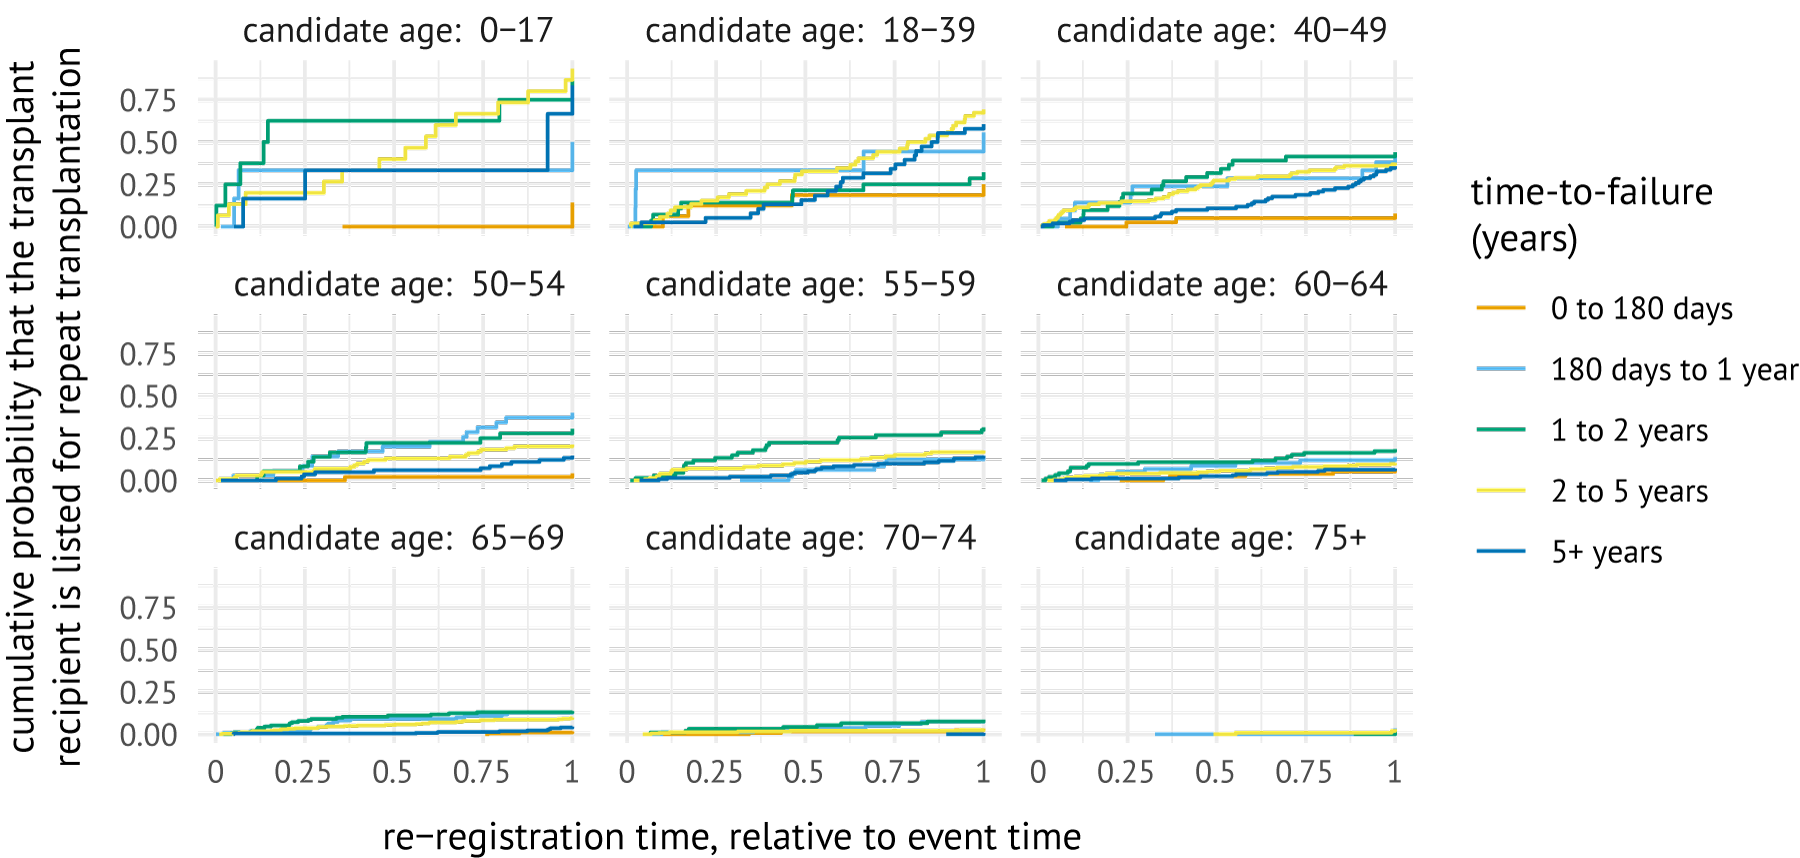
\includegraphics[width=1\linewidth]{figures/ch8//sFig1} 

}

\caption{Cumulative incidence curves showing the probability of listing for repeat transplantation, stratified by time-to-event categories. These curves were estimated with the Kaplan-Meier estimator based on candidates transplanted between January 1, 2011, and January 1, 2024.}\label{fig:ch8sfig1}
\end{figure}

\subsubsection{Constructing synthetic re-registrations}\label{sec:etkidneysynthreg}

In case transplant recipients are simulated to enlist for a repeat
transplantation before the simulation end date, the post-transplant
module creates a \emph{synthetic re-listing} for this candidate. This
synthetic re-listing is created by combining the static information from
the transplant recipient with the dynamic candidate status updates from
an actually re-listed candidate. The actually re-listed candidate is
chosen such that they are similar to transplant recipient in terms of
background characteristics as well as in time-to-failure \(t\) and time-to-relisting
\(r\).

By default, the post-transplant module finds a matching re-registration
\(k\) by:

\begin{enumerate}
\def\labelenumi{\arabic{enumi}.}
\item
  Considering re-listings where candidates match on country of listing and on
  whether they were re-listed within 1 year after transplantation\footnote{Transplant
    recipients who require dialysis within one year of their initial kidney
    transplant may receive a portion of their previous waiting time back, see
    the Eurotransplant kidney manual \citep{manualKidney}.}, are of similar age (\textless20 years difference), have similar time
  to re-listing and time-to-failure, and have a similar number
  of years on dialysis.
\item
  Selecting the m=5 listings for repeat transplantation with the closest Mahalanobis
  distance between (\(r_i\), \(t_i\)) and (\(r_k\), \(t_k\)).
\item
  Sampling a random re-registration from the \(m\) re-registrations.
\end{enumerate}

A synthetic re-registration is then constructed by combining patient
attributes from patient \(i\) with the urgency code updates and PRA re-certifications
from patient \(k\). These status updates affect whether a candidate is eligible for a match
list offer, as candidates with a non-transplantable status or outdated PRA screenings
are not eligible for offers in ETKAS and ESP. Other status updates (vPRA, allocation profiles,
diagnosis groups, HLA, reported dialysis initiation dates) are not copied over
because they are considered patient-specific. We note that the PRA screenings
are only used to determine the eligibility of the candidate, and not to predict
graft offer acceptance behavior or post-transplant survival.

A specific challenge for simulating listing for repeat transplantation is that
kidney transplantation is a strongly immunizing event \citep{Lopes2015}. Many
repeat transplant candidates will therefore have
developed \emph{de novo} Donor-Specific Antibodies (dnDSAs) that centers can report as
unacceptable. Candidates who are listed for repeat transplantation
therefore tend to have higher vPRAs and face reduced access to kidney transplantation.
\newpage
It is not clear how to simulate such \emph{de novo} immunization, because:

\begin{itemize}
\item
  HLA antigens are cross-reactive, which means that patients typically also
  develop DSAs against HLA antigens that were not present in the donor \citep{Lucas2015},
\item
  the immunogenicity of donor HLAs also depends on the patient's own HLA
  \citep{Lucas2015}, and
\item
  HLA laboratories and transplant centers have different attitudes in
  labeling the HLA antigens of the initial donor as unacceptable \citep{Susal2013, Ziemann2022}.
\end{itemize}

Accurate simulation of \emph{de novo} immunization falls outside of the scope of
the ETKidney simulator. Instead, a very simple procedure was
implemented that assumes that candidates have a fixed probability
of becoming immunized against any mismatched donor antigen. By default,
this probability is set to 20\%. This probability was chosen because
having one additional mismatch per locus increases the probability of
reporting unacceptable antigens against that specific locus with 10 to 25\%
on average (depending on the locus) \citep{Isaacson2022}.

\section{Verification and validation}\label{sec:etkidneyvv}

This section describes verification and validation efforts undertaken to
ensure that the ETKidney simulator closely mimics ETKAS and ESP.

\subsection{Verification of the ETKidney simulator}\label{sec:etkidneyverification}

We built unit tests to ensure that the behavior of the modules aligns
with their intended functionality. For example, unit tests were
constructed to verify whether HLA match qualities returned by the HLA
system module were equal to HLA match qualities recorded on actual ETKAS match lists.
Unit tests were also used to ascertain that the HLA system module
returned the correct mismatch probabilities and vPRAs.

The simulation of the graft offering process and of post-transplant survival
is based on statistical models whose parameters were estimated in the statistical
programming language \emph{R}. Unit tests were constructed to ensure that the
probabilities predicted in the ETKidney simulator based on these parameters matched
the probabilities predicted in R, for both offer acceptance
decisions as well as post-transplant survival.
\vfill
\newpage

\subsection{Validation of the ETKidney simulator}\label{sec:etkidneyvalidation}

To ensure face validity of the model, medical doctors from
Eurotransplant were actively involved in the development and conceptual
design of the simulator. We also had meetings with ETKAC and the ETRL on
various occasions in which the ETKidney simulator was discussed. Moreover,
the model was presented at the 2024 Eurotransplant Annual Meeting to
collect feedback from additional major stakeholders,
such as medical doctors and transplantation coordinators affiliated with the
transplant centers.

We assess the operational validity of the model using input-output validation.
For this, we simulate ETKAS and ESP kidney
allocation between April 1, 2021, and January 1, 2024 under the actual allocation
rules used within this simulation window. The simulation start date of April 1, 2021
was chosen because the allocation of ESP donors changed in March 2021.
For the donor input stream, we
used all 4,326 donors reported in the simulation window
whose kidneys were transplanted after allocation through ETKAS or ESP (see Table \ref{tab:ch8tab1donors}
for their characteristics). For the candidate input stream, we used all
n=9,393 candidates activated on the ETKAS or ESP waiting list during the
simulation period (Table \ref{tab:ch8tab1patlisted}), and the n=14,647
candidates already registered candidates on April 1, 2021
(Table \ref{tab:ch8tab1patsimstart}).

\begin{table}[!h]
\centering
\caption{\label{tab:ch8tab1donors}Characteristics of the donors used for simulation.}
\centering
\resizebox{\ifdim\width>\linewidth\linewidth\else\width\fi}{!}{
\fontsize{10}{12}\selectfont
\begin{tabular}[t]{>{\centering\arraybackslash}p{6em}cccccccc}
\toprule
variable & level & \makecell{Austria\\(n=372)} & \makecell{Belgium\\(n=627)} & \makecell{Croatia\\(n=189)} & \makecell{Germany\\(n=2,072)} & \makecell{Hungary\\(n=265)} & \makecell{Netherlands\\(n=704)} & \makecell{Slovenia\\(n=97)}\\
\midrule
 & 2 & 260 (69.9\%) & 471 (75.1\%) & 127 (67.2\%) & 1,625 (78.4\%) & 208 (78.5\%) & 532 (75.6\%) & 71 (73.2\%)\\
\cmidrule{2-9}
\multirow{-2}{6em}[1\dimexpr\aboverulesep+\belowrulesep+\cmidrulewidth]{\centering\arraybackslash kidneys available} & 1 & 112 (30.1\%) & 156 (24.9\%) & 62 (32.8\%) & 447 (21.6\%) & 57 (21.5\%) & 172 (24.4\%) & 26 (26.8\%)\\
\cmidrule{1-9}
 & HB & 350 (94.1\%) & 345 (55.0\%) & 189 (100\%) & 2,072 (100\%) & 265 (100\%) & 260 (36.9\%) & 97 (100\%)\\
\cmidrule{2-9}
\multirow{-2}{6em}[1\dimexpr\aboverulesep+\belowrulesep+\cmidrulewidth]{\centering\arraybackslash type} & NHB & 22 (5.9\%) & 282 (45.0\%) & – & – & – & 444 (63.1\%) & –\\
\cmidrule{1-9}
 & female & 166 (44.6\%) & 256 (40.8\%) & 75 (39.7\%) & 965 (46.6\%) & 113 (42.6\%) & 314 (44.6\%) & 28 (28.9\%)\\
\cmidrule{2-9}
\multirow{-2}{6em}[1\dimexpr\aboverulesep+\belowrulesep+\cmidrulewidth]{\centering\arraybackslash sex} & male & 206 (55.4\%) & 371 (59.2\%) & 114 (60.3\%) & 1,107 (53.4\%) & 152 (57.4\%) & 390 (55.4\%) & 69 (71.1\%)\\
\cmidrule{1-9}
 & 0-17 years & 22 (5.9\%) & 16 (2.6\%) & 15 (7.9\%) & 85 (4.1\%) & 12 (4.5\%) & 12 (1.7\%) & 9 (9.3\%)\\
\cmidrule{2-9}
 & 18-49 years & 118 (31.7\%) & 235 (37.5\%) & 69 (36.5\%) & 650 (31.4\%) & 136 (51.3\%) & 191 (27.1\%) & 34 (35.1\%)\\
\cmidrule{2-9}
 & 50-64 years & 166 (44.6\%) & 264 (42.1\%) & 70 (37.0\%) & 786 (37.9\%) & 100 (37.7\%) & 291 (41.3\%) & 37 (38.1\%)\\
\cmidrule{2-9}
\multirow{-4}{6em}[3\dimexpr\aboverulesep+\belowrulesep+\cmidrulewidth]{\centering\arraybackslash age} & 65+ years & 66 (17.7\%) & 112 (17.9\%) & 35 (18.5\%) & 551 (26.6\%) & 17 (6.4\%) & 210 (29.8\%) & 17 (17.5\%)\\
\cmidrule{1-9}
 & O & 136 (36.6\%) & 260 (41.5\%) & 60 (31.7\%) & 784 (37.8\%) & 67 (25.3\%) & 329 (46.7\%) & 35 (36.1\%)\\
\cmidrule{2-9}
 & A & 168 (45.2\%) & 285 (45.5\%) & 91 (48.1\%) & 914 (44.1\%) & 121 (45.7\%) & 279 (39.6\%) & 43 (44.3\%)\\
\cmidrule{2-9}
 & B & 45 (12.1\%) & 69 (11.0\%) & 28 (14.8\%) & 270 (13.0\%) & 51 (19.2\%) & 74 (10.5\%) & 14 (14.4\%)\\
\cmidrule{2-9}
\multirow{-4}{6em}[3\dimexpr\aboverulesep+\belowrulesep+\cmidrulewidth]{\centering\arraybackslash ABO blood group} & AB & 23 (6.2\%) & 13 (2.1\%) & 10 (5.3\%) & 104 (5.0\%) & 26 (9.8\%) & 22 (3.1\%) & 5 (5.2\%)\\
\cmidrule{1-9}
 & anoxia & 63 (16.9\%) & 227 (36.2\%) & 14 (7.4\%) & 452 (21.8\%) & 39 (14.7\%) & 190 (27.0\%) & 13 (13.4\%)\\
\cmidrule{2-9}
 & CVA & 232 (62.4\%) & 262 (41.8\%) & 129 (68.3\%) & 1,180 (56.9\%) & 175 (66.0\%) & 362 (51.4\%) & 47 (48.5\%)\\
\cmidrule{2-9}
 & trauma & 75 (20.2\%) & 121 (19.3\%) & 39 (20.6\%) & 375 (18.1\%) & 48 (18.1\%) & 136 (19.3\%) & 34 (35.1\%)\\
\cmidrule{2-9}
\multirow{-4}{6em}[3\dimexpr\aboverulesep+\belowrulesep+\cmidrulewidth]{\centering\arraybackslash death cause} & other & 2 (0.5\%) & 17 (2.7\%) & 7 (3.7\%) & 65 (3.1\%) & 3 (1.1\%) & 16 (2.3\%) & 3 (3.1\%)\\
\bottomrule
\end{tabular}}
\parbox{\textwidth}{\footnotesize \smallskip Based on donors reported between April 1, 2021, and December 31, 2024, who had their kidneys allocated and transplanted via ETKAS or ESP. Abbreviations: HB, heartbeating; NHB, nonheartbeating}
\end{table}

\begin{table}[!h]
\centering
\caption{\label{tab:ch8tab1patlisted}Characteristics of newly registered patients who were used for simulations.}
\centering
\resizebox{\ifdim\width>\linewidth\linewidth\else\width\fi}{!}{
\fontsize{10}{12}\selectfont
\begin{tabular}[t]{>{\centering\arraybackslash}p{6em}cccccccc}
\toprule
variable & level & \makecell{Austria\\(n=859)} & \makecell{Belgium\\(n=1,461)} & \makecell{Croatia\\(n=352)} & \makecell{Germany\\(n=4,547)} & \makecell{Hungary\\(n=665)} & \makecell{Netherlands\\(n=1,406)} & \makecell{Slovenia\\(n=103)}\\
\midrule
 & primary & 721 (83.9\%) & 1,278 (87.5\%) & 328 (93.2\%) & 3,978 (87.5\%) & 609 (91.6\%) & 1,173 (83.4\%) & 88 (85.4\%)\\
\cmidrule{2-9}
\multirow{-2}{6em}[1\dimexpr\aboverulesep+\belowrulesep+\cmidrulewidth]{\centering\arraybackslash type transplant} & repeat & 138 (16.1\%) & 183 (12.5\%) & 24 (6.8\%) & 569 (12.5\%) & 56 (8.4\%) & 233 (16.6\%) & 15 (14.6\%)\\
\cmidrule{1-9}
 & 0-17 years & 22 (2.6\%) & 35 (2.4\%) & 7 (2.0\%) & 252 (5.5\%) & 28 (4.2\%) & 15 (1.1\%) & 3 (2.9\%)\\
\cmidrule{2-9}
 & 18-49 years & 279 (32.5\%) & 467 (32.0\%) & 124 (35.2\%) & 1,617 (35.6\%) & 283 (42.6\%) & 351 (25.0\%) & 44 (42.7\%)\\
\cmidrule{2-9}
 & 50-64 years & 376 (43.8\%) & 616 (42.2\%) & 155 (44.0\%) & 1,898 (41.7\%) & 270 (40.6\%) & 562 (40.0\%) & 35 (34.0\%)\\
\cmidrule{2-9}
\multirow{-4}{6em}[3\dimexpr\aboverulesep+\belowrulesep+\cmidrulewidth]{\centering\arraybackslash age} & 65+ years & 182 (21.2\%) & 343 (23.5\%) & 66 (18.8\%) & 780 (17.2\%) & 84 (12.6\%) & 478 (34.0\%) & 21 (20.4\%)\\
\cmidrule{1-9}
 & O & 332 (38.6\%) & 656 (44.9\%) & 132 (37.5\%) & 1,730 (38.0\%) & 182 (27.4\%) & 617 (43.9\%) & 42 (40.8\%)\\
\cmidrule{2-9}
 & A & 365 (42.5\%) & 583 (39.9\%) & 130 (36.9\%) & 1,962 (43.1\%) & 303 (45.6\%) & 522 (37.1\%) & 44 (42.7\%)\\
\cmidrule{2-9}
 & B & 108 (12.6\%) & 159 (10.9\%) & 72 (20.5\%) & 618 (13.6\%) & 121 (18.2\%) & 210 (14.9\%) & 14 (13.6\%)\\
\cmidrule{2-9}
\multirow{-4}{6em}[3\dimexpr\aboverulesep+\belowrulesep+\cmidrulewidth]{\centering\arraybackslash ABO blood group} & AB & 54 (6.3\%) & 63 (4.3\%) & 18 (5.1\%) & 237 (5.2\%) & 59 (8.9\%) & 57 (4.1\%) & 3 (2.9\%)\\
\cmidrule{1-9}
 & 0\% & 675 (78.6\%) & 1,059 (72.5\%) & 221 (62.8\%) & 3,249 (71.5\%) & 510 (76.7\%) & 1,016 (72.3\%) & 72 (69.9\%)\\
\cmidrule{2-9}
 & >0-84.9\% & 134 (15.6\%) & 298 (20.4\%) & 101 (28.7\%) & 970 (21.3\%) & 94 (14.1\%) & 282 (20.1\%) & 20 (19.4\%)\\
\cmidrule{2-9}
\multirow{-3}{6em}[2\dimexpr\aboverulesep+\belowrulesep+\cmidrulewidth]{\centering\arraybackslash vPRA at listing} & 85+\% & 50 (5.8\%) & 104 (7.1\%) & 30 (8.5\%) & 328 (7.2\%) & 61 (9.2\%) & 108 (7.7\%) & 11 (10.7\%)\\
\cmidrule{1-9}
 & on dialysis & 803 (93.5\%) & 1,247 (85.4\%) & 327 (92.9\%) & 4,479 (98.5\%) & 586 (88.1\%) & 1,057 (75.2\%) & 96 (93.2\%)\\
\cmidrule{2-9}
\multirow{-2}{6em}[1\dimexpr\aboverulesep+\belowrulesep+\cmidrulewidth]{\centering\arraybackslash dialysis status} & preemptive & 56 (6.5\%) & 214 (14.6\%) & 25 (7.1\%) & 68 (1.5\%) & 79 (11.9\%) & 349 (24.8\%) & 7 (6.8\%)\\
\cmidrule{1-9}
\makecell{dial. time\\at listing} & mean [Q1-Q3] & 1.7 [0.5-2.3] & 1.3 [0.0-1.7] & 1.6 [0.4-2.4] & 2.4 [0.8-3.0] & 1.2 [0.1-1.5] & 1.0 [0.0-1.1] & 2.4 [0.7-2.9]\\
\bottomrule
\end{tabular}}
\parbox{\textwidth}{\footnotesize \smallskip Based on patients listed in ETKAS or ESP between Apr 1, 2021 and December 31, 2024, with at least one active status in this period.}
\end{table}

\begin{table}[!h]
\centering
\caption{\label{tab:ch8tab1patsimstart}Characteristics of patients already present on the waiting list on April 1, 2021.}
\centering
\resizebox{\ifdim\width>\linewidth\linewidth\else\width\fi}{!}{
\fontsize{10}{12}\selectfont
\begin{tabular}[t]{>{\centering\arraybackslash}p{6em}cccccccc}
\toprule
variable & level & \makecell{Austria\\(n=807)} & \makecell{Belgium\\(n=1,223)} & \makecell{Croatia\\(n=374)} & \makecell{Germany\\(n=9,513)} & \makecell{Hungary\\(n=1,006)} & \makecell{Netherlands\\(n=1,631)} & \makecell{Slovenia\\(n=93)}\\
\midrule
 & active & 563 (69.8\%) & 907 (74.2\%) & 135 (36.1\%) & 6,480 (68.1\%) & 770 (76.5\%) & 712 (43.7\%) & 46 (49.5\%)\\
\cmidrule{2-9}
\multirow{-2}{6em}[1\dimexpr\aboverulesep+\belowrulesep+\cmidrulewidth]{\centering\arraybackslash \makecell{status\\}} & inactive & 244 (30.2\%) & 316 (25.8\%) & 239 (63.9\%) & 3,033 (31.9\%) & 236 (23.5\%) & 919 (56.3\%) & 47 (50.5\%)\\
\cmidrule{1-9}
 & primary & 581 (72.0\%) & 972 (79.5\%) & 304 (81.3\%) & 7,813 (82.1\%) & 941 (93.5\%) & 1,321 (81.0\%) & 74 (79.6\%)\\
\cmidrule{2-9}
\multirow{-2}{6em}[1\dimexpr\aboverulesep+\belowrulesep+\cmidrulewidth]{\centering\arraybackslash type transplant} & repeat & 226 (28.0\%) & 251 (20.5\%) & 70 (18.7\%) & 1,700 (17.9\%) & 65 (6.5\%) & 310 (19.0\%) & 19 (20.4\%)\\
\cmidrule{1-9}
 & 0-17 years & 5 (0.6\%) & 16 (1.3\%) & 5 (1.3\%) & 159 (1.7\%) & 14 (1.4\%) & 9 (0.6\%) & 0 (0\%)\\
\cmidrule{2-9}
 & 18-49 years & 264 (32.7\%) & 433 (35.4\%) & 144 (38.5\%) & 3,334 (35.0\%) & 404 (40.2\%) & 392 (24.0\%) & 36 (38.7\%)\\
\cmidrule{2-9}
 & 50-64 years & 401 (49.7\%) & 532 (43.5\%) & 149 (39.8\%) & 4,639 (48.8\%) & 402 (40.0\%) & 691 (42.4\%) & 40 (43.0\%)\\
\cmidrule{2-9}
\multirow{-4}{6em}[3\dimexpr\aboverulesep+\belowrulesep+\cmidrulewidth]{\centering\arraybackslash \makecell{age\\}} & 65+ years & 137 (17.0\%) & 242 (19.8\%) & 76 (20.3\%) & 1,381 (14.5\%) & 186 (18.5\%) & 539 (33.0\%) & 17 (18.3\%)\\
\cmidrule{1-9}
 & O & 408 (50.6\%) & 654 (53.5\%) & 145 (38.8\%) & 4,216 (44.3\%) & 368 (36.6\%) & 826 (50.6\%) & 38 (40.9\%)\\
\cmidrule{2-9}
 & A & 239 (29.6\%) & 332 (27.1\%) & 133 (35.6\%) & 3,468 (36.5\%) & 372 (37.0\%) & 478 (29.3\%) & 24 (25.8\%)\\
\cmidrule{2-9}
 & B & 131 (16.2\%) & 200 (16.4\%) & 75 (20.1\%) & 1,383 (14.5\%) & 206 (20.5\%) & 278 (17.0\%) & 22 (23.7\%)\\
\cmidrule{2-9}
\multirow{-4}{6em}[3\dimexpr\aboverulesep+\belowrulesep+\cmidrulewidth]{\centering\arraybackslash ABO blood group} & AB & 29 (3.6\%) & 37 (3.0\%) & 21 (5.6\%) & 446 (4.7\%) & 60 (6.0\%) & 49 (3.0\%) & 9 (9.7\%)\\
\cmidrule{1-9}
 & 0\% & 479 (59.4\%) & 694 (56.7\%) & 189 (50.5\%) & 5,573 (58.6\%) & 717 (71.3\%) & 1,085 (66.5\%) & 50 (53.8\%)\\
\cmidrule{2-9}
 & >0-84.9\% & 209 (25.9\%) & 299 (24.4\%) & 100 (26.7\%) & 2,650 (27.9\%) & 173 (17.2\%) & 337 (20.7\%) & 19 (20.4\%)\\
\cmidrule{2-9}
\multirow{-3}{6em}[2\dimexpr\aboverulesep+\belowrulesep+\cmidrulewidth]{\centering\arraybackslash vPRA group} & 85+\% & 119 (14.7\%) & 230 (18.8\%) & 85 (22.7\%) & 1,290 (13.6\%) & 116 (11.5\%) & 209 (12.8\%) & 24 (25.8\%)\\
\cmidrule{1-9}
 & on dialysis & 789 (97.8\%) & 1,164 (95.2\%) & 358 (95.7\%) & 9,497 (99.8\%) & 924 (91.8\%) & 1,455 (89.2\%) & 90 (96.8\%)\\
\cmidrule{2-9}
\multirow{-2}{6em}[1\dimexpr\aboverulesep+\belowrulesep+\cmidrulewidth]{\centering\arraybackslash dialysis status} & preemptive & 18 (2.2\%) & 59 (4.8\%) & 16 (4.3\%) & 16 (0.2\%) & 82 (8.2\%) & 176 (10.8\%) & 3 (3.2\%)\\
\cmidrule{1-9}
\makecell{dial. years\\dial. } & mean [Q1-Q3] & 3.2 [1.5-4.2] & 3.1 [1.1-4.1] & 3.4 [1.6-4.2] & 5.7 [3.1-7.7] & 3.0 [1.2-4.3] & 1.9 [0.0-2.8] & 4.0 [1.8-5.5]\\
\bottomrule
\end{tabular}}
\parbox{\textwidth}{\footnotesize \smallskip Based on patients listed in ETKAS or ESP before Apr 1, 2024, with at least one active status in this period.}
\end{table}

\FloatBarrier

To enable accurate simulation of the ETKAS balance system, we also
exported from the Eurotransplant database all cross-border transplantations that
followed allocation via the AM program or were a combined transplantation. These
transplantations were used to define the input stream of international transplantations. In
simulations, we schedule donor arrivals, candidate status updates, and balance
update events on the dates this information was actually reported to
Eurotransplant. Our input-output validation exercise thus keeps the
inputs as close as possible to reality, and assesses whether the outputs of
the ETKidney simulator are comparable to the actual outputs of ETKAS and
ESP.

Importantly, the outputs of the simulator depend on several stochastic
processes: the offer acceptance behavior of the transplant centers,
listing for a repeat transplantation after an initial kidney transplantation,
and the switching to non-standard allocation by Eurotransplant. To give insight into variability of simulator
outputs, we simulate ETKAS and ESP allocation 200 times over the
simulation window and report 95\% interquantile ranges for relevant
summary statistics. These 95\% IQRs are obtained by simulating allocation
200 times and reporting the 2.5th and 97.5th percentiles of simulation
outputs. For each of these 200 simulation runs, we use a different set
of completed status trajectories (see Section \ref{sec:etkidneyinputstreams}). We say that the ETKidney
simulator is \emph{``well-calibrated''} for a quantity of interest if the
observed summary statistic falls within the 95\% IQR of the 200
simulations.

\subsubsection*{Results of input-output validation}\label{sec:etkidneyioval}
\addcontentsline{toc}{subsubsection}{Results of input-output validation}

Table \ref{tab:ch8tab1} reports results of this input-output validation for kidney waiting list outcomes.
The ETKidney simulator
is well-calibrated for almost all summary statistics: the total number
of transplantations, the number of dual kidney transplantations, the
number of ETKAS or ESP transplantations, the number of re-listings, and
the number of waiting list deaths per country in all countries. We only
observe miscalibration for the number of waiting list deaths in Hungary
(-11\%) and the active waiting list size at simulation termination (2\%
too many candidates have an active waiting list status).
\newpage
Table \ref{tab:ch8tab2} reports input-output validation
results for ETKAS and ESP transplantations. For ETKAS, the simulator is
well-calibrated for the number of transplantations placed by allocation mechanism
(standard or non-standard), transplantations by candidate age group, and
transplantations in repeat transplant candidates. The simulator is
also well-calibrated for the number of transplantations by HLA match
quality, with only the number of zero-mismatched transplantations
overestimated (\Plus 5\%). The number of
transplantations in candidates with vPRAs exceeding 95\% is
underestimated (-17\%). This miscalibration appears to have been the result
of the introduction of the virtual crossmatch in January 2023, potentially
because the number of positive crossmatches in the recipient center decreased
after the introduction of the
virtual crossmatch in Eurotransplant \citep{Heidt2024} (see Table \ref{tab:ch8stab1} for miscalibration after January 2023). The simulator is well-calibrated
for the number of transplantations per country, with only a slight
overestimation observed in Croatia (\Plus 3\%) and a slight
underestimation observed in Hungary (-2\%). The degree of geographical sharing
is underestimated in ETKAS: there are too many local or regional transplantations
in simulations (\Plus 5\%), and too few inter-regional (-11\%) or international
(-9\%) transplantations.

Table \ref{tab:ch8tab2} also shows that the ETKidney simulator is
well-calibrated for most relevant outcomes in ESP: the number of transplantations in
primary and repeat kidney transplant candidates, and the number of
transplantations by HLA match quality and immunization status. The simulator
overestimates the number of kidneys transplanted after non-standard allocation
in ESP (+23\%). An apparent consequence of this is that the number of
kidneys allocated to candidates under the age of 65 is overestimated
(\Plus 28\%), particularly in Belgium, the
Netherlands, and Slovenia where
centers appear to be reluctant to transplant a candidate under the age of 65
with an ESP donor (see Table \ref{tab:ch8stab2}). Finally, the simulator is well-calibrated for the
number of transplantations by recipient country and match geography,
with the only exception Germany where 2\% too many ESP kidneys are
transplanted.

\newpage
Overall, the ETKidney simulator appears to be well-calibrated for most
outcomes of ETKAS and ESP allocation. The results of this input-output
validation exercise were discussed with medical doctors from
Eurotransplant and ETKAC, who deemed differences small enough to make
the simulator useful for determining the impact of alternative kidney
allocation policies. We illustrate this with case studies in the next
section.

\FloatBarrier

\begin{table}[h]
\caption{Input-output validation of waiting list outcomes between April 1, 2021 and January 1, 2024. For simulations, the numbers shown are the averages and 95\% interquantile ranges (IQR) of outcomes over 200 simulations. Ranges are displayed in bold if the simulator is not well-calibrated, i.e. the actual statistic does not fall within the 95\% IQR.}
\label{tab:ch8tab1}
\centering
\resizebox{1\ifdim\width>\linewidth\linewidth\else\width\fi}{!}{%
\begin{tabular}{L{4.9cm} R{5.2cm} L{2cm}}
\toprule
\multirow[b]{1.5}{*}{category} & \multirow[b]{1.5}{*}{\makecell{simulated results\\(average and 95\% IQR)}} & \multirow[b]{1.5}{*}{\makecell{actual data\\(2021-2024)}}\\
& & \vspace{-0em} \\
\midrule
\addlinespace[0.3em]
\multicolumn{3}{l}{\textbf{transplantations through ETKAS or ESP}}\\
\hspace{1em}number of unique donors & 4326 & 4326\\
\hspace{1em}number of transplantations & 7546   [7530-7560] & 7549\\
\addlinespace[0.3em]
\multicolumn{3}{l}{\textbf{number of transplantations by type}}\\
\hspace{1em}single kidney & 7471   [7440-7500] & 7484\\
\hspace{1em}dual kidney & 74     [60-90] & 65\\
\addlinespace[0.3em]
\multicolumn{3}{l}{\textbf{number of transplantations by allocation mechanism}}\\
\hspace{1em}ESP & 1740   [1727-1752] & 1745\\
\hspace{1em}ETKAS & 5805   [5797-5814] & 5804\\
\addlinespace[0.3em]
\multicolumn{3}{l}{\textbf{waiting list}}\\
\hspace{1em}initial active waiting list & 9589 & 9589\\
\hspace{1em}number of listings & 24028  [24010-24046] & 24038\\
\hspace{1em}re-listings in simulated period & 106    [88-124] & 116\\
\hspace{1em}final active waiting list size & \textbf{10142  [\Plus2\%, 10095-10194]} & 9958\\
\hspace{1em}waiting list removals (count) & 1449   [1427-1473] & 1469\\
\hspace{1em}waiting list deaths (count) & 1146   [1122-1165] & 1140\\
\addlinespace[0.3em]
\multicolumn{3}{l}{\textbf{number of waiting list deaths by country}}\\
\hspace{1em}Austria & 73     [67-80] & 73\\
\hspace{1em}Belgium & 82     [73-90] & 73\\
\hspace{1em}Croatia & 40     [36-46] & 40\\
\hspace{1em}Germany & 723    [705-740] & 713\\
\hspace{1em}Hungary & \textbf{128    [-11\%, 121-135]} & 144\\
\hspace{1em}Netherlands & 92     [84-99] & 90\\
\hspace{1em}Slovenia & 7      [5-10] & 7\\
\bottomrule
\end{tabular}
}
\end{table}

\begin{table}[h]
\caption{Validation of the number of transplantations between April 1, 2021, and January 1, 2024. For simulations, the numbers shown are averages and 95\% IQRs over 200 simulations. Statistics are displayed in bold if the actual value does not fall within the 95\% IQR.}
\label{tab:ch8tab2}
\centering
\resizebox{1\ifdim\width>\linewidth\linewidth\else\width\fi}{!}{%
\hspace*{-.03\linewidth}
\centering
\setlength{\tabcolsep}{3pt}
\begin{tabular}{L{3.4cm} R{4cm} L{.9cm} R{4.1cm} L{.9cm}}
\toprule
\multicolumn{1}{c}{ } & \multicolumn{2}{c}{ETKAS} & \multicolumn{2}{c}{ESP} \\
\cmidrule(l{3pt}r{3pt}){2-3} \cmidrule(l{3pt}r{3pt}){4-5}
\multirow[b]{1.5}{*}{category} & \multirow[b]{1.5}{*}{\makecell{simulated results\\(average and 95\% IQR)}} & \multirow[b]{1.5}{*}{actual} & \multirow[b]{1.5}{*}{\makecell{simulated results\\(average and 95\% IQR)}} & \multirow[b]{1.5}{*}{actual}\\
& & & & \vspace{-0em} \\


\midrule
\addlinespace[0.3em]
\multicolumn{5}{l}{\textbf{allocation mechanism}}\\
\hspace{.7em}standard & 5044   [4881-5169] & 5000 & \textbf{1117   [-10\%, 1049-1188]} & 1237\\
\hspace{.7em}non-standard & 761    [632-915] & 804 & \textbf{623    [\Plus23\%, 551-690]} & 508\\
\addlinespace[0.3em]
\multicolumn{5}{l}{\textbf{recipient characteristics}}\\
\hspace{.7em}pediatric recipient & 339    [321-358] & 325 & 0 & 0\\
\hspace{.7em}aged 65 or over & 734    [700-769] & 725 & \textbf{1512   [-4\%, 1475-1548]} & 1567\\
\hspace{.7em}aged below 65 & 5071   [5034-5105] & 5079 & \textbf{228    [\Plus28\%, 192-261]} & 178\\
\hspace{.7em}primary transplant & 5038   [5001-5068] & 5039 & 1661   [1644-1677] & 1665\\
\hspace{.7em}repeat transplant & 768    [734-795] & 765 & 80     [67-92] & 80\\
\addlinespace[0.3em]
\multicolumn{5}{l}{\textbf{HLA-ABDR mismatches}}\\
\hspace{.7em}0 ABDR & \textbf{650    [\Plus5\%, 624-675]} & 617 & 3      [1-6] & 4\\
\hspace{.7em}0 or 1 BDR & 1136   [1083-1179] & 1153 & 62     [50-77] & 55\\
\hspace{.7em}1B\Plus1DR or 2 B\Plus0 DR & 2468   [2406-2534] & 2492 & 316    [285-348] & 336\\
\hspace{.7em}2DR or 3\Plus \ BDR & 1551   [1490-1609] & 1542 & 1360   [1328-1388] & 1350\\
\addlinespace[0.3em]
\multicolumn{5}{l}{\textbf{sensitization status (vPRA)}}\\
\hspace{.7em}0\% & \textbf{4211   [\Plus2\%, 4173-4255]} & 4142 & 1477   [1455-1502] & 1468\\
\hspace{.7em}0.01-84.9\% & 1320   [1279-1356] & 1355 & 256    [233-278] & 264\\
\hspace{.7em}85-94.9\% & 173    [155-191] & 186 & 6      [2-10] & 9\\
\hspace{.7em}95\Plus\% & \textbf{101    [-17\%, 87-114]} & 121 & \textbf{2      [-50\%, 1-3]} & 4\\
\addlinespace[0.3em]
\multicolumn{5}{l}{\textbf{recipient country}}\\
\hspace{.7em}Austria & 532    [525-538] & 530 & 106    [87-128] & 118\\
\hspace{.7em}Belgium & 912    [905-918] & 914 & 107    [83-132] & 120\\
\hspace{.7em}Croatia & \textbf{277    [\Plus3\%, 272-283]} & 270 & 38     [26-51] & 26\\
\hspace{.7em}Germany & 2648   [2635-2659] & 2651 & \textbf{1081   [\Plus3\%, 1049-1118]} & 1048\\
\hspace{.7em}Hungary & \textbf{464    [-2\%, 457-470]} & 472 & 19     [11-28] & 24\\
\hspace{.7em}Netherlands & 854    [847-860] & 849 & 380    [349-406] & 398\\
\hspace{.7em}Slovenia & 119    [113-124] & 118 & 9      [4-15] & 11\\
\addlinespace[0.3em]
\multicolumn{5}{l}{\textbf{match geography}}\\
\hspace{.7em}local or regional & \textbf{4087   [\Plus5\%, 3993-4164]} & 3902 & 1374   [1324-1424] & 1408\\
\hspace{.7em}interregional & \textbf{637    [-11\%, 590-680]} & 715 & 174    [138-206] & 178\\
\hspace{.7em}international & \textbf{1081   [-9\%, 1012-1164]} & 1187 & 192    [153-225] & 159\\
\bottomrule
\end{tabular}
}
\end{table}

\begin{table}[h]
\caption{Input-output validation of the number of transplantations by vPRA, before
and after the introduction of the virtual crossmatch on January 24, 2023.}
\label{tab:ch8stab1}
\centering
\resizebox{1\ifdim\width>\linewidth\linewidth\else\width\fi}{!}{%

\begin{tabular}{rrlrl}
\toprule
\multicolumn{1}{c}{ } & \multicolumn{2}{c}{before virtual crossmatch} & \multicolumn{2}{c}{after virtual crossmatch} \\
\cmidrule(l{3pt}r{3pt}){2-3} \cmidrule(l{3pt}r{3pt}){4-5}
vPRA (\%) & \makecell{simulated\\(mean and 95\% IQR)} & actual & \makecell{simulated\\(mean and 95\% IQR)} & actual\\
\midrule
0\% & 2751 [2711-2792] & 2755 & \textbf{1460 [1428-1489]} & 1387\\
0.01-84.9\% & 875 [842-909] & 861 & \textbf{446 [417-474]} & 494\\
85-94.9\% & 114 [99-128] & 117 & 59 [48-69] & 69\\
95+\% & 67 [56-78] & 75 & \textbf{34 [25-44]} & 46\\
\bottomrule
\end{tabular}
}
\end{table}

\begin{table}[h]
\caption{Input-output validation of the number of transplantations with ESP donors in
candidates under the age of 65, by recipient country of listing.}
\label{tab:ch8stab2}
\centering
\resizebox{1\ifdim\width>\linewidth\linewidth\else\width\fi}{!}{%

\begin{tabular}{rrl}
    \toprule
    \multicolumn{1}{c}{ } & \multicolumn{2}{c}{\makecell{number of ESP transplantations\\in candidates aged below 65}} \\
    \cmidrule(l{3pt}r{3pt}){2-3}
    country of listing & \makecell{simulated\\(mean and 95\% IQR)} & actual\\
    \midrule
    Austria & 19 [12-28] & 20\\
    Belgium & \textbf{14 [6-23]} & 3\\
    Croatia & 13 [7-21] & 8\\
    Germany & 156 [131-184] & 139\\
    Hungary & 3 [1-6] & 6\\
    Netherlands & \textbf{18 [8-30]} & 1\\
    Slovenia & \textbf{5 [2-10]} & 1\\
    \bottomrule
\end{tabular}
}
\end{table}

\FloatBarrier

\section{Case studies}\label{sec:etkidneycasestudies}

Together with ETKAC, three topics for case studies were selected in
which the ETKidney simulator could help quantify the impact of
alternative kidney allocation rules. The selected
topics all concern the ETKAS program, and are (i) emphasizing matching at the HLA-B and HLA-DR locus,
(ii) the introduction of a sliding scale based on
the vPRA, and (iii) candidate-donor age matching. To limit the effects of
transient effects, we extend the simulation period for these case
studies from January 1, 2016 to January 1, 2024. We simulate all policy
alternatives 20 times, and use traditional hypothesis testing to assess
whether alternative policies significantly change the outcomes compared
to the current policy. To increase the power of these tests, we use common
random numbers \citep{lawSimulationModelingAnalysis2015} as a variance
reduction technique. Consequently, the outcomes that are simulated under the
alternative allocation rules can be compared to the outcomes simulated under
the current rules with pairwise t-tests.

\subsection{Case study 1: emphasizing matching at HLA-B and HLA-DR loci}\label{sec:etkidneycasestudyhla}

Since its initiation in 1996, the ETKAS point system has placed equal emphasis
on matching at the HLA-A, HLA-B, and HLA-DR loci, despite broad
consensus that HLA-DR mismatches are more deleterious to graft survival
than HLA-A and HLA-B mismatches
\citep{vereerstraetenExperienceWujciakOpelzAllocation1998, Roberts2004}.
Internal analyses on registry data from Eurotransplant suggest that
mismatches on the HLA-B and HLA-DR locus are indeed more strongly associated with graft
loss than mismatches on the HLA-A locus. This motivated us to simulate
policies that emphasize matching at the HLA-B and HLA-DR loci relative to the
HLA-A locus.

The current ETKAS point system awards 400 points for HLA matching and
penalizes HLA mismatches on the A, B, and DR loci with 66.7 points per
mismatch. We assess the impact of three alternative HLA matching
policies. These policies all continue to award up to 400 points for
candidate-donor HLA match quality, but shift weight from the HLA-A
locus to the HLA-B and HLA-DR loci (see Table \ref{tab:ch8tab3}).
The first policy is referred
to as the \(\text{B} + 2\text{DR}\) policy, because it gives no weight to
the HLA-A locus, maintains the same weight for the HLA-B locus (-66.7 points),
and doubles the weight on the HLA-DR locus (-133.3 points). The second
policy, referred to as the \(0.5\text{A} + \text{B} + 1.5\text{DR}\)
policy, shifts only half of the weight placed on the HLA-A locus to the HLA-DR
locus. The final policy, referred to as
\(1.5\texttt{B} + 1.5\texttt{DR}\), penalizes mismatches at the HLA-B and HLA-DR
loci both with 100 points per mismatch.

\begingroup
\setlength{\aboverulesep}{0.2ex}
\setlength{\belowrulesep}{0.1ex}

\begin{table}[h]
\caption{Overview of the points awarded per locus for the alternative HLA-matching policies.}
\label{tab:ch8tab3}
\centering
\resizebox{0.94\ifdim\width>\linewidth\linewidth\else\width\fi}{!}{%
    \begin{tabular}{@{}cccc@{}}
        \toprule
        policy & HLA-A &
        HLA-B & HLA-DR \\
        \midrule
        current & -66.7     & -66.7     & -66.7\\
        B + 2DR & 0     & -66.7     & -133.3 \\
        $0.5$A + B + $1.5$DR & -33.3 & -66.7     & -100 \\
        $1.5$B + $1.5$DR & 0     & -100     & -100\\
        \bottomrule
    \end{tabular}
}
\end{table}

\FloatBarrier

Simulation results for these three alternative policies are summarized
in Table \ref{tab:ch8tab4}. These results show that the policy
alternatives reduce the number of transplantations with 2 DR or 3 or more B\Plus DR mismatches by 25 to 39\%, and
increase the number of transplantations with 1 B or 1 DR mismatch by 26
to 49\%. Thus, the policies indeed succeed in improving match quality on
the HLA-B and HLA-DR locus.

\begin{table}[h]
\caption{The simulated change in the number of transplantations under alternative HLA-ABDR matching policies. The numbers displayed are the averages of the differences observed over 20 simulations. mm: mismatches.}
\label{tab:ch8tab4}
\centering
\resizebox{1\ifdim\width>\linewidth\linewidth\else\width\fi}{!}{%
\begin{tabular}{l@{}cclrlrl}
\toprule
\multicolumn{2}{c}{ } & \multicolumn{6}{c}{\multirow[b]{1.5}{*}{\makecell{change in number of transplantations\\compared to current policy}}} \\
& & & & \vspace{-0em} \\
\cmidrule(l{3pt}r{3pt}){3-8}
& \makecell{average number of \\transplantations\\observed under\\the current policy}
    & \multicolumn{2}{c}{B + 2DR} 
    & \multicolumn{2}{c}{0.5A + B + 1.5DR}  
    & \multicolumn{2}{c}{1.5B + 1.5DR} \\
\midrule
\addlinespace[0.3em]
\multicolumn{8}{l}{\textbf{By HLA-ABDR mismatch count}}\\
\hspace{.5em}0   & 1925 & -9 & (-0\%) & -1 & (-0\%) & -6 & (-0\%) \\
\hspace{.5em}1   & 952  & -181$^{\dagger\dagger\dagger}$ & (-19\%) & -55$^{\dagger\dagger\dagger}$ & (-6\%) & -99$^{\dagger\dagger\dagger}$ & (-10\%) \\
\hspace{.5em}2   & 3855 & -634$^{\dagger\dagger\dagger}$ & (-16\%) & -252$^{\dagger\dagger\dagger}$ & (-7\%) & -509$^{\dagger\dagger\dagger}$ & (-13\%) \\
\hspace{.5em}3   & 6037 & -358$^{\dagger\dagger\dagger}$ & (-6\%)  & -76$^{\dagger\dagger\dagger}$  & (-1\%)  & -224$^{\dagger\dagger\dagger}$ & (-4\%)  \\
\hspace{.5em}4   & 3235 & \Plus 837$^{\dagger\dagger\dagger}$ & (\Plus 26\%) & \Plus 282$^{\dagger\dagger\dagger}$ & (\Plus 9\%)  & \Plus 642$^{\dagger\dagger\dagger}$ & (\Plus 20\%) \\
\hspace{.5em}5   & 730  & \Plus 340$^{\dagger\dagger\dagger}$ & (\Plus 47\%) & \Plus 104$^{\dagger\dagger\dagger}$ & (\Plus 14\%) & \Plus 191$^{\dagger\dagger\dagger}$ & (\Plus 26\%) \\
\hspace{.5em}6   & 78   & \Plus 2                       & (\Plus 3\%)  & 0                              & (0\%)      & \Plus 7$^{\dagger}$            & (\Plus 9\%)  \\
\addlinespace[0.3em]
\multicolumn{8}{l}{\textbf{By HLA-ABDR match quality}}\\
\hspace{.5em}000         & 1925 & -9 & (-0\%)  & -1 & (-0\%)  & -6 & (-0\%)  \\
\hspace{.5em}*00, *10, *01 & 3264 & \Plus 1364$^{\dagger\dagger\dagger}$ & (\Plus 42\%) & \Plus 850$^{\dagger\dagger\dagger}$ & (\Plus 26\%) & \Plus 1585$^{\dagger\dagger\dagger}$ & (\Plus 49\%) \\
\hspace{.5em}*20, *11   & 7234 & \Plus 209$^{\dagger\dagger\dagger}$  & (\Plus 3\%)  & \Plus 240$^{\dagger\dagger\dagger}$ & (\Plus 3\%)  & \Plus 131$^{\dagger\dagger\dagger}$ & (\Plus 2\%)  \\
\hspace{.5em}**2, *21   & 4388 & -1567$^{\dagger\dagger\dagger}$ & (-36\%) & -1087$^{\dagger\dagger\dagger}$ & (-25\%) & -1708$^{\dagger\dagger\dagger}$ & (-39\%) \\
\addlinespace[0.3em]
\multicolumn{8}{l}{\textbf{By homozygosity of the candidate the HLA-B and HLA-DR locus}}\\
\hspace{.5em}B and DR & 473  & -39$^{\dagger\dagger\dagger}$ & (-8\%)  & -17$^{\dagger\dagger\dagger}$ & (-4\%)  & -30$^{\dagger\dagger\dagger}$ & (-6\%)  \\
\hspace{.5em}DR       & 1662 & -207$^{\dagger\dagger\dagger}$ & (-12\%) & -104$^{\dagger\dagger\dagger}$ & (-6\%)  & -94$^{\dagger\dagger\dagger}$ & (-6\%)  \\
\hspace{.5em}B        & 1052 & \Plus 31$^{\dagger\dagger\dagger}$ & (\Plus 3\%)  & \Plus 14$^{\dagger\dagger}$       & (\Plus 1\%)  & -19$^{\dagger\dagger\dagger}$       & (-2\%)  \\
\hspace{.5em}none     & 13625& \Plus 212$^{\dagger\dagger\dagger}$ & (\Plus 2\%)  & \Plus 110$^{\dagger\dagger\dagger}$ & (\Plus 1\%)  & \Plus 144$^{\dagger\dagger\dagger}$ & (\Plus 1\%)  \\
\bottomrule
\end{tabular}
}
\parbox{\textwidth}{\footnotesize \smallskip $\qquad\qquad$ $^{\dagger}$ p < 0.05, $^{\dagger\dagger}$ p < 0.01, $^{\dagger\dagger\dagger}$ p < 0.001}
\end{table}

\endgroup
\FloatBarrier

However, results also show that there are unintended consequences of
this policy: the total number of ABDR mismatches at transplantation
increases with all alternative policies and there are 5 to 12\% fewer
transplantations in candidates who have homozygosity at the HLA-B or HLA-DR
loci, who are already disadvantaged in the current ETKAS system. Results
such as those presented in Table \ref{tab:ch8tab4} can facilitate discussions by ETKAC
on whether the improved match quality at HLA-B and HLA-DR loci is worth the increase
in total mismatches and the reduced access to kidney transplants for homozygotes.

\subsection{Case study 2: a sliding scale for the vPRA}\label{sec:etkidneycasestudyvpra}

Prior studies have suggested that immunized candidates have reduced
access to transplantation in ETKAS (see \citep{ziemannUnacceptableHumanLeucocyte2017, zecherImpactSensitizationWaiting2022a} and Chapter \ref{CHvpra}).
In this case study, we assess whether this disparity can be alleviated
by awarding points directly for the vPRA. For this, we modify the ETKAS point
system in two ways. The first modification is that we directly award points for
the vPRA using a \emph{sliding scale}. Such a sliding scale for the vPRA has been a part of
kidney allocation in the United States since 2014 \citep{stewartSmoothingItOut2012}.
The number of points awarded based on this sliding scale is calculated as \[\texttt{weight}\cdot\frac{\texttt{base}^{\texttt{vPRA}}}{\texttt{base}-1}.\]
The maximum number of points awarded by the sliding scale depends on its \emph{weight},
and its steepness depends on the \emph{base}. The second modification is that we no longer directly award points for the vPRA via the mismatch probability.
Instead, we replace mismatch probability points by the 1-ABDR HLA mismatch frequency (see Section \ref{sec:etkidneymmp}). This quantity awards points to candidates based on
how difficult-to-match their HLA phenotype is, and not their blood group or
their vPRA.

Representatives of ETKAC reached consensus that the aim of the
sliding scale should be that a candidate's chance of being transplanted
through ETKAS should not decline up to a vPRA of 85\%. Above this vPRA,
candidates could have access to the AM program, or should consider removing unacceptable antigens in case they do not
meet AM criteria. We used the ETKidney simulator to simulate ETKAS for
different combinations of weights and bases,
and quantify the association between vPRA and the relative
transplant rate using Cox proportional hazards model on the outcomes simulated
by the ETKidney simulator. For this, the same model specification is used as in Chapter
\ref{CHvpra}. In Figure
\ref{fig:ch8fig4} the estimated relation between vPRA and the transplant rate is
shown for several sliding scales. From this figure, the sliding scale
with a base of 5 and weight of 133 appears to be the most acceptable
option: with this sliding scale, the relative transplant rate
of sensitized candidates no longer decays until a vPRA of 85\%, as was desired
by ETKAC.

\begin{figure}[ht]

{\centering 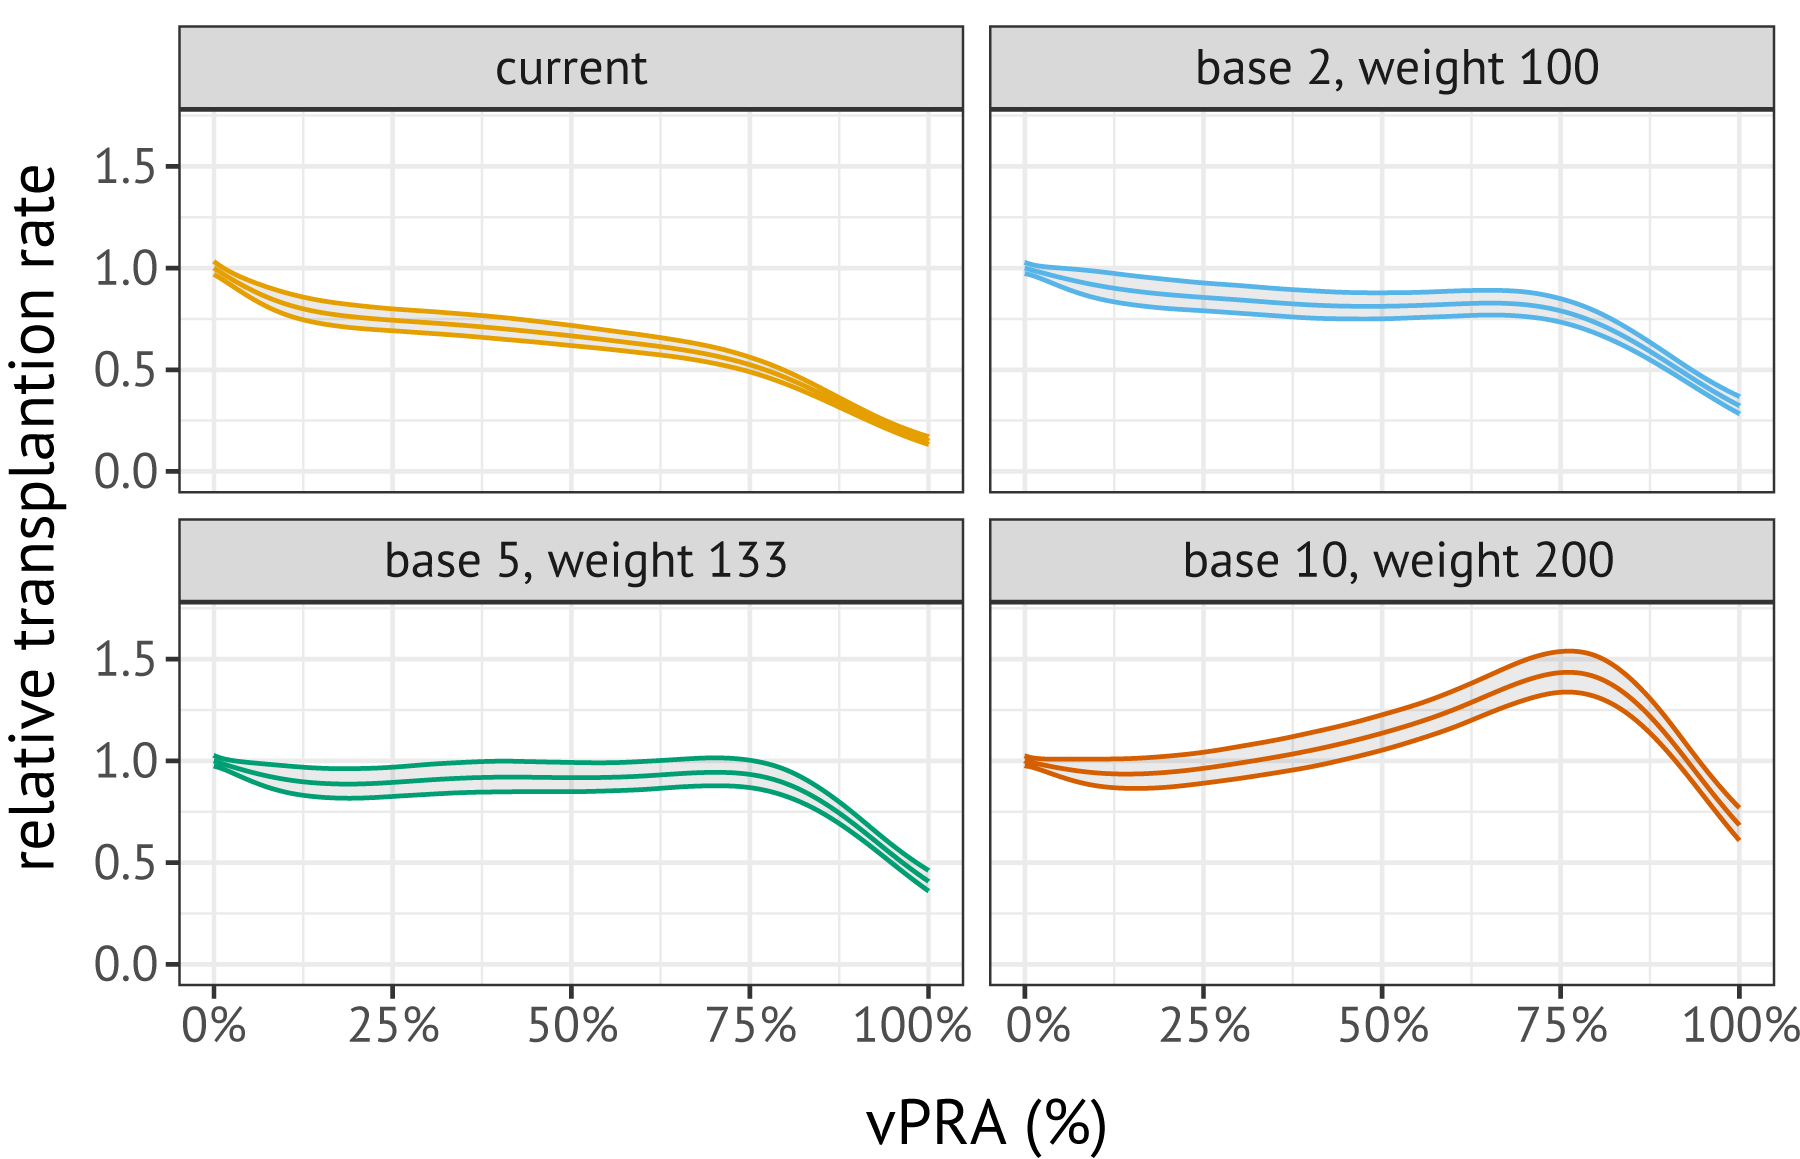
\includegraphics[width=0.85\linewidth]{figures/ch8//fig4-vpra_effect} 

}

\caption{Relations between the relative transplant rate and the vPRA in ETKAS, estimated on ETKidney simulator outcomes. These relations were estimated with a Cox proportional hazards model, using a spline transformation for the vPRA.}\label{fig:ch8fig4}
\end{figure}

\FloatBarrier

\subsection{Case study 3: candidate-donor age matching}\label{sec:etkidneycasestudyagematching}

Consensus in the transplantation literature is that kidneys procured
from young donors should preferentially be transplanted in young
candidates
\citep{waiserAgeMatchingRenal2000, pippiasYoungDeceasedDonor2020, vanittersumIncreasedRiskGraft2017, coemansCompetingRisksModel2024, keithEffectDonorRecipient2004b}.
While allocation systems in France and the United Kingdom have implemented mechanisms that explicitly award points for
continuous candidate-donor age matching
\citep{Audry2022, watson2020overview}, the
ETKAS point system does not award points based on candidate or donor age
(except for bonus points that are given to pediatric patients). In this case study, we (i) use retrospective data
from Eurotransplant to quantify the associations of candidate and donor age with patient and graft survival
with cause-specific
hazard models, and (ii) simulate and evaluate two age matching policies
for ETKAS.

To quantify the relation between donor or candidate age and
post-transplant survival, we consider all patients transplanted with a
kidney through ETKAS or ESP between 2004 and 2019. We exclude candidates
with the HU status and candidates without any follow-up information
(n = 7,458), leaving n = 36,576 transplantations. We fit
cause-specific Cox proportional hazards models on these transplantations
for (i) graft loss and (ii) death with a functioning graft. We censored
both time-to-event variables ten years after transplantation, because
completeness of follow-up data beyond this time
horizon is poor (available for less than 30\% of patients). Besides donor and candidate age, we adjust for
donor characteristics (DCD/DCD donation, hypertension,
last creatinine, death cause, diabetes, malignancy), candidate
characteristics (dialysis time), and match characteristics (a zero-mismatch
indicator, the number of mismatches per locus for the HLA-A, -B, and -DR loci, and
match geography). To allow for non-linear relations between continuous
variables and the hazard rate, we adjust for spline transformations of
the continuous variables. The estimated relations between donor or
candidate age and patient and graft survival are shown in Figure \ref{fig:ch8fig5}. These results are qualitatively
similar to results obtained by Coemans et al. \citep{coemansCompetingRisksModel2024},
who report that the hazard rate of graft loss decays linearly with
recipient age while it increases quadratically with donor age, and that
the mortality hazard rate increases quadratically with candidate age (note that the y-axis for the second panel is shown on the logarithmic scale).

\begin{figure}[ht]

{\centering 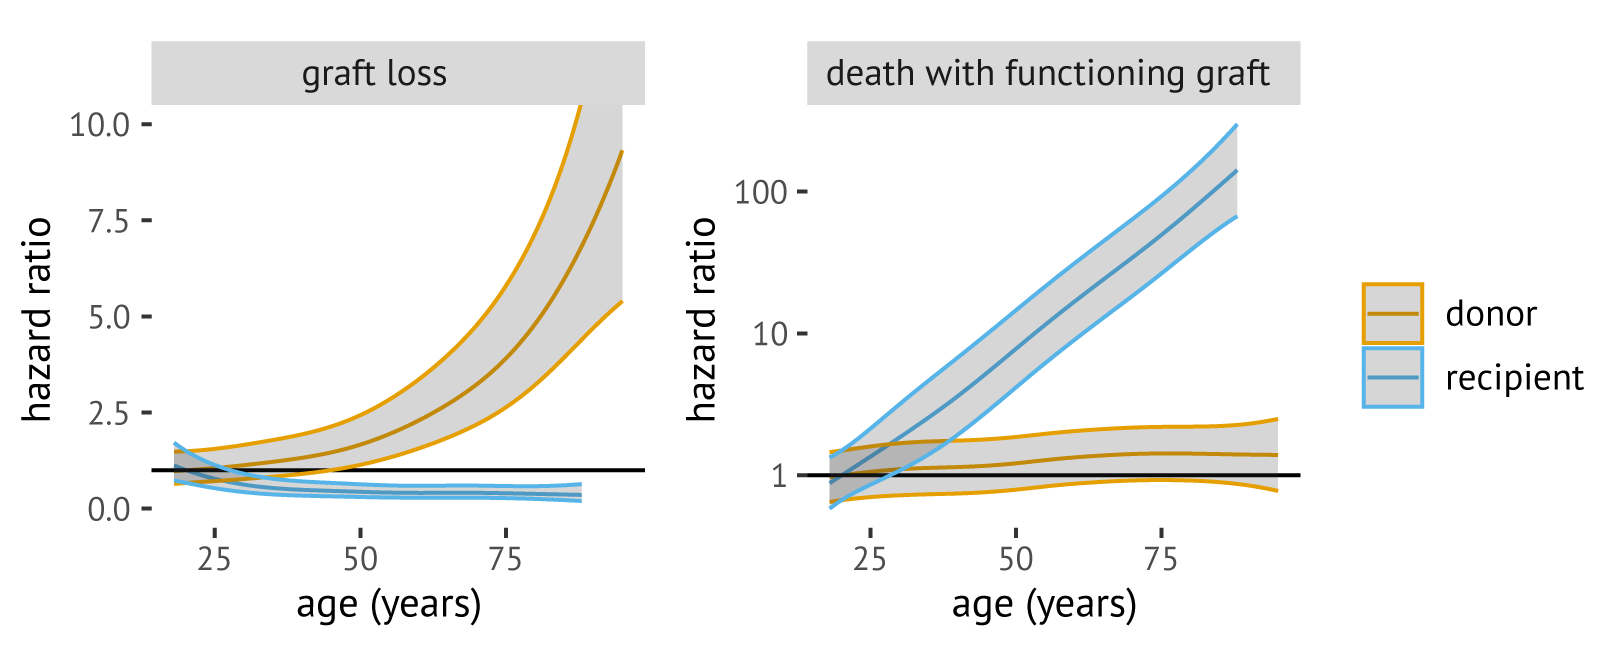
\includegraphics[width=1\linewidth]{figures/ch8//fig5-competing_risk_model} 

}

\caption{Estimated relations between graft loss and death with a functioning graft. Note that the hazard ratio for death with a functioning graft is shown on the logarithmic scale.}\label{fig:ch8fig5}
\end{figure}

We simulate two candidate-donor age matching policies, both
inspired by the French kidney allocation policy that was introduced in 2015
\citep{Audry2022}. Like ETKAS, the French policy awards
points for candidate waiting time, HLA matching between the donor and candidate,
the candidate's likelihood of being favorably matched with a kidney, and the geographic distance
between the donor and candidate. However, in France an ``age filter'' is
applied to the total number of points awarded, with candidates ranked based on
the filtered number of points. For example, the French age filter is 0\%
for a candidate who is over 20 years older than the donor, which
means that such candidates receive 0\% of their total points for ranking.
The French age filter is asymmetrical with allocation of kidneys from
a young donor to an older patient discouraged more strongly than
the allocation of a kidney from an older donor to a young candidate.

Inspired by this French age filter, we evaluate two asymmetrical age filters for ETKAS
(see Figure \ref{fig:ch8fig6}). Both filters give a candidate 100\%
of their ETKAS points in case the age difference between the candidate and donor is 5 years or less. The ``strict'' filter (blue) is similar to the
French age filter in that it gives almost no points in case the
candidate is much older than the donor. The ``muted'' filter (orange)
gives a larger fraction of the total number of ETKAS points, which we
anticipated to be more acceptable for Eurotransplant because it
maintains a better balance in the international exchange of kidneys.

\begin{figure}[ht]

{\centering 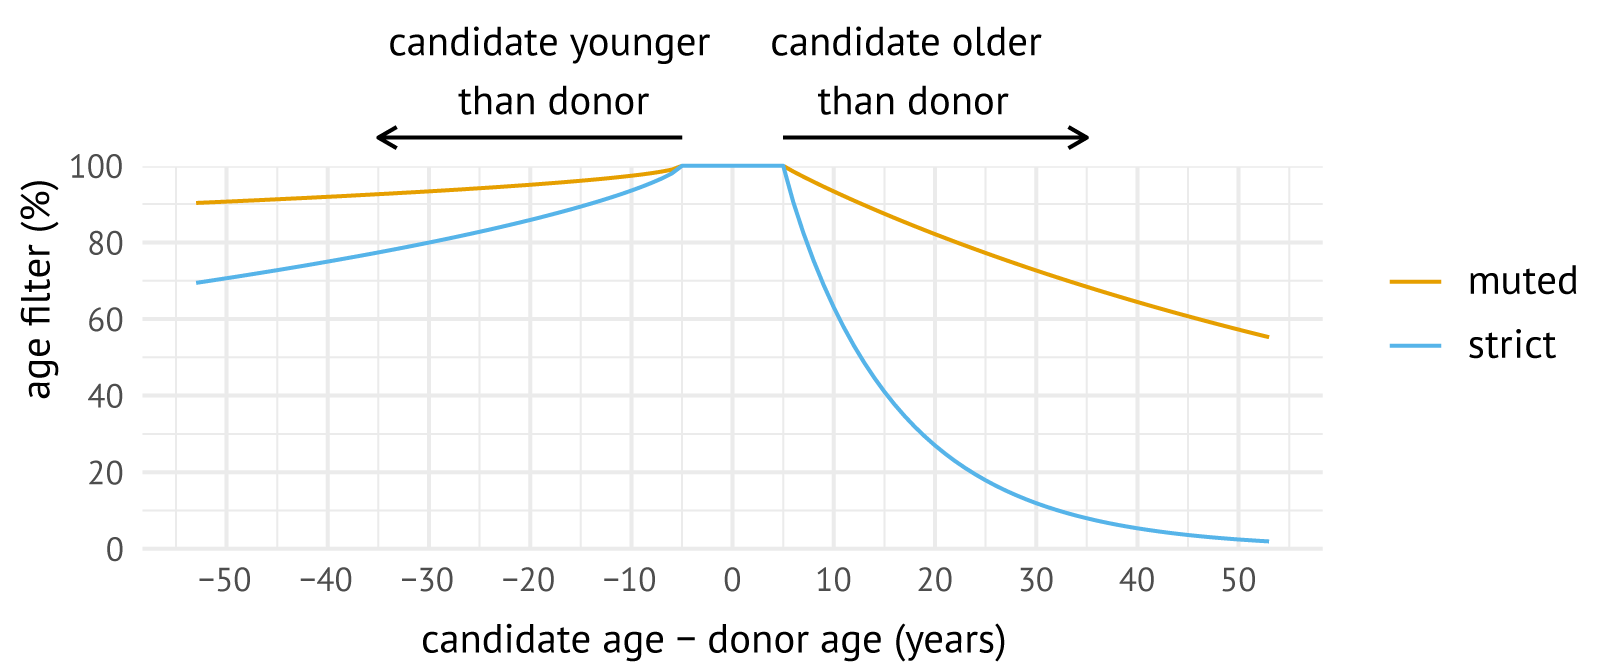
\includegraphics[width=1\linewidth]{figures/ch8//fig6-age_matching_policies} 

}

\caption{Evaluated age filters for ETKAS.}\label{fig:ch8fig6}
\end{figure}

Simulated outcomes for the muted and strict age matching policies are
compared to the current policy in Table
\ref{tab:ch8tab5}. The table shows that the muted
and strict policies increase the number of age-matched transplantations (defined as
transplantations with a candidate-donor age difference of at most five years) by 60\% and 138\%, respectively.
An unintended consequence is that the muted and strict age filters lead to reduced
HLA match quality at transplantation, with a 12\% and 33\% increase
in the number of level 4 mismatched kidney transplantations (2 DR, or 3 or 4 B+DR
mismatches), respectively. Table also
\ref{tab:ch8tab5} shows that the muted policy
only modestly increases international sharing (+5\%) and inter-regional
sharing (+7\%), while the strict policy leads to a 37\% increase in
international transplantations. The
strict age filter increases the number of extended or rescue
transplantations (+7\%), potentially because international offers are
relatively more likely to be declined.

To evaluate whether the benefits of candidate-donor age matching outweigh
its unintended consequences, we use the earlier mentioned cause-specific
hazard models to predict the probability of death with a functioning
graft ten years after transplantation for all simulated
transplantations. For this, we predict the cumulative incidence of death
with functioning graft using a cause-specific hazards approach \citep{wreedeMstatePackageAnalysis2011}. By summing up these 10-year event probabilities
for all candidates, we obtain the expected number of events ten years after
transplantation, which is visualized in Figure \ref{fig:ch8fig7} for the current policy
(green), the muted age filter (orange), and the strict age filter
(blue). These results suggest that the muted and strict age filter could
reduce the numbers of deaths with a functioning graft 10 years after
transplantation by 11\% and 18\%, respectively.

\begin{table}[h]
\caption{The simulated change in the number of transplantations in ETKAS under continuous candidate-donor age matching policies. The numbers displayed are the average differences over 20 simulations. mm: mismatches.}
\label{tab:ch8tab5}
\centering
\resizebox{1\ifdim\width>\linewidth\linewidth\else\width\fi}{!}{%
\begin{tabular}{lcrlrl}
    \toprule
    \multicolumn{2}{c}{ } & \multicolumn{4}{c}{\multirow[b]{1.5}{*}{\makecell{change in number of transplantations\\compared to current policy}}} \\
    & & & & & \vspace{-0em} \\
    \cmidrule(l{3pt}r{3pt}){3-6}
      & \makecell{average number of \\transplantations observed \\under the current policy}
    & \multicolumn{2}{c}{muted age filter}
    & \multicolumn{2}{c}{strict age filter} \\
\midrule
\addlinespace[0.3em]
\multicolumn{6}{l}{\textbf{age difference}}\\
\hspace{1em}candidate 35+ years older        & 708   & -497$^{***}$ & (-70\%)  & -557$^{***}$ & (-79\%) \\
\hspace{1em}candidate 15-34 years older      & 3166  & -1742$^{***}$ & (-55\%)  & -2549$^{***}$ & (-81\%) \\
\hspace{1em}candidate 6-14 years older       & 3256  & +434$^{***}$  & (+13\%)  & -1756$^{***}$ & (-54\%) \\
\hspace{1em}max 5 year difference            & 4810  & +2919$^{***}$ & (+61\%)  & +6640$^{***}$ & (+138\%) \\
\hspace{1em}candidate 6-14 years younger     & 2624  & -151$^{***}$  & (-6\%)   & -230$^{***}$  & (-9\%)  \\
\hspace{1em}candidate 15-34 years younger    & 2064  & -873$^{***}$  & (-42\%)  & -1386$^{***}$ & (-67\%) \\
\hspace{1em}candidate 35+ years younger      & 184   & -86$^{***}$   & (-47\%)  & -155$^{***}$  & (-84\%) \\
\addlinespace[0.3em]
\multicolumn{6}{l}{\textbf{HLA match quality}}\\
\hspace{1em}level 1 (0 ABDR mm)              & 1922  & -8           & (-0\%)   & -40$^{***}$   & (-2\%)  \\
\hspace{1em}level 2 (at most 1 BDR mm)       & 3250  & -380$^{***}$ & (-12\%)  & -902$^{***}$  & (-28\%) \\
\hspace{1em}level 3 (2B or 1DR+1B mm)        & 7224  & -156$^{***}$ & (-2\%)   & -496$^{***}$  & (-7\%)  \\
\hspace{1em}level 4 (2DR or 3\Plus\ BDR mm)   & 4417  & +547$^{***}$ & (+12\%)  & +1446$^{***}$ & (+33\%) \\
\addlinespace[0.3em]
\multicolumn{6}{l}{\textbf{match geography}}\\
\hspace{1em}local or regional                & 11744 & -297$^{***}$ & (-3\%)   & -1514$^{***}$ & (-13\%) \\
\hspace{1em}national                         & 1796  & +121$^{***}$ & (+7\%)   & +306$^{***}$  & (+17\%) \\
\hspace{1em}international                    & 3272  & +179$^{***}$ & (+5\%)   & +1215$^{***}$ & (+37\%) \\
\addlinespace[0.3em]
\multicolumn{6}{l}{\textbf{type of allocation}}\\
\hspace{1em}standard allocation              & 14487 & +50          & (+0\%)   & -160*         & (-1\%)  \\
\hspace{1em}non-standard                     & 2325  & -47          & (-2\%)   & +167$^{*}$    & (+7\%)  \\
\bottomrule
\end{tabular}
}
\parbox{\textwidth}{\footnotesize \smallskip $^{*}$ p < 0.05, $^{**}$ p < 0.01, $^{***}$ p < 0.001}
\end{table}

\FloatBarrier

\begin{figure}[h]

{\centering 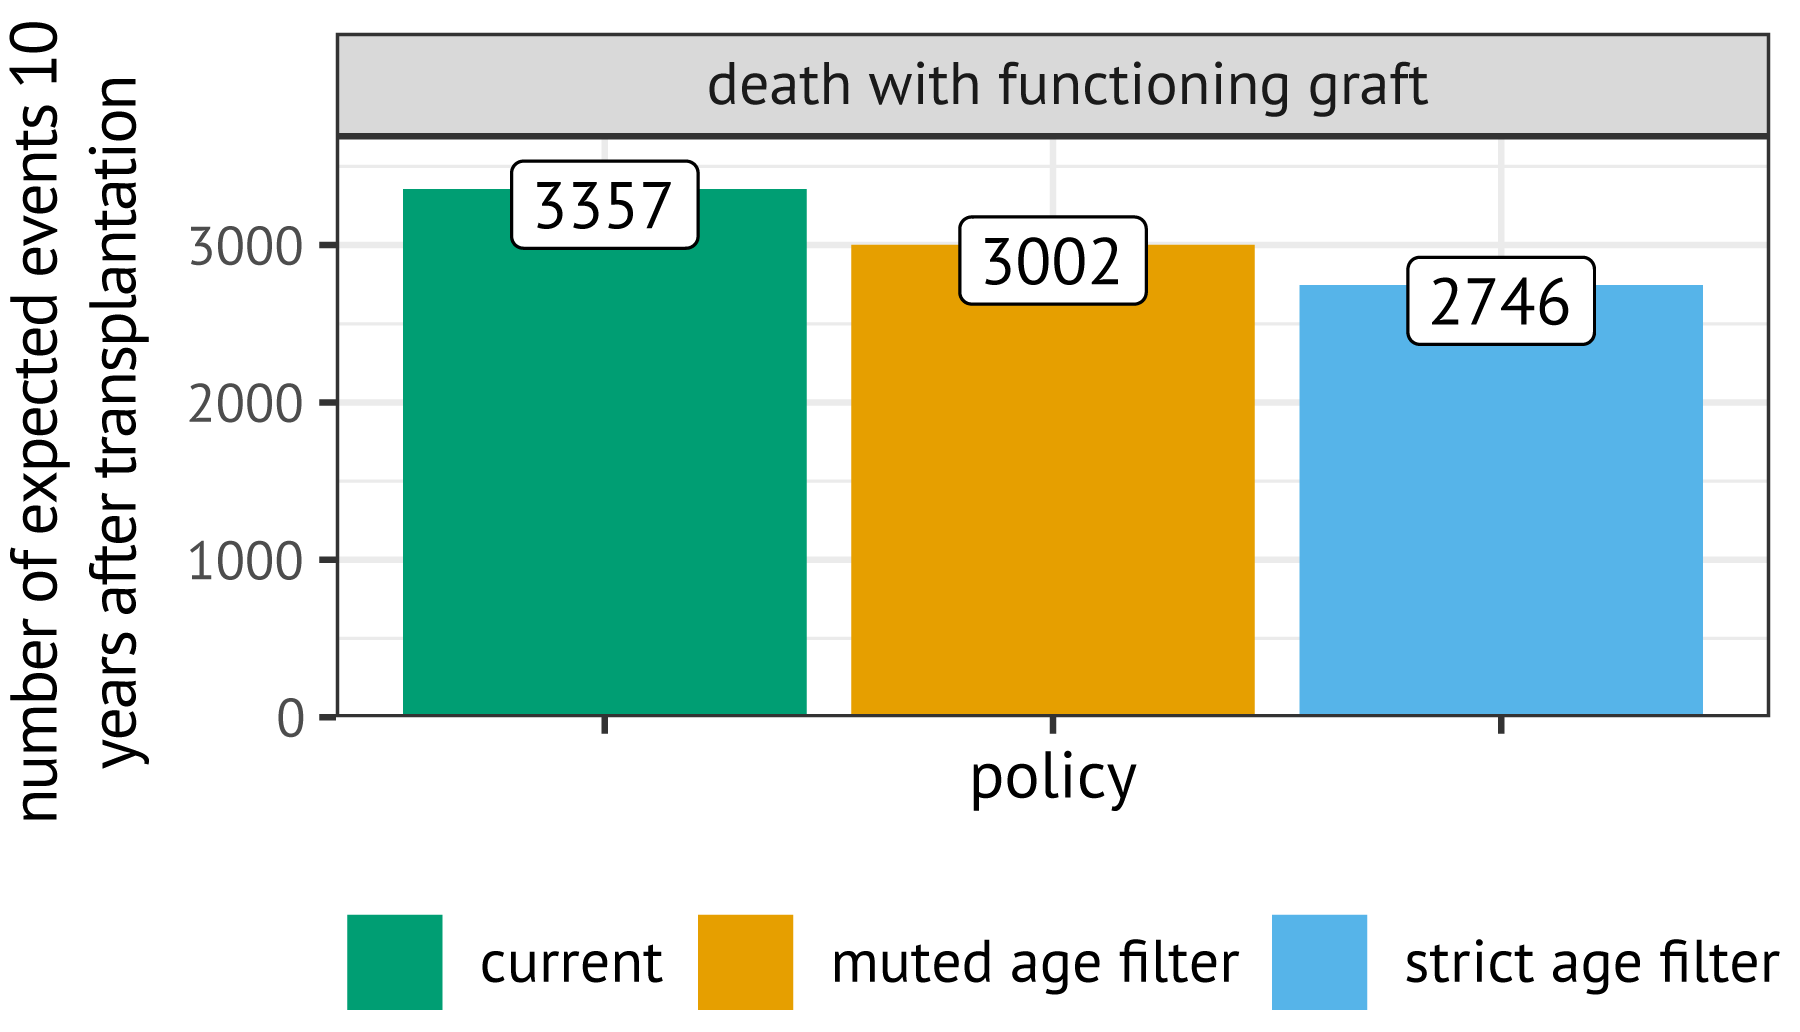
\includegraphics[width=0.65\linewidth]{figures/ch8//fig7-posttransplantevents} 

}

\caption{Expected number of post-transplant events ten years after transplantation, predicted based on candidate, donor, and transplantation characteristics with competing risk models.}\label{fig:ch8fig7}
\end{figure}

\FloatBarrier

\section{Discussion and conclusion}\label{sec:etkidneydiscussion}

Eurotransplant has long recognized the important role computer simulations could have for
allocation development. For example, in the one-year evaluation of ETKAS that was
published in 1998, the organization stressed that \emph{``introduction of a change must be
preceded by a computer simulation study''}
\citep{demeesterNewEurotransplantKidney1998}. However, Eurotransplant has
only recently started the development of tools required for such
simulation studies, with initiatives including the development of the ELAS simulator
(see Chapter \ref{CHelassimulator}) and the passing a recommendation by the Thoracic
Committee to develop a simulation tool for heart and lung allocation in 2024.
Within this line of research, we present the ETKidney
simulator.

Discrete-event simulators are already routinely used to update allocation rules in other
geographic regions
\citep{Pritsker1995, Mumford2018, jacquelinetChangingKidneyAllocation2006}.
The most prominent simulator for kidney allocation is the Kidney-Pancreas Simulated Allocation
Model (KPSAM), which was developed to simulate kidney allocation in the United States and which is made publicly available for research by the SRTR. KPSAM differs
from the ETKidney simulator in several aspects. Firstly, KPSAM users have to
manually specify in simulation inputs when a candidate would list for a
repeat transplantation, as well as how their statuses would
evolve after their return to the waiting list; in the ETKidney simulator, simulation of re-listings is instead
based on historical data. Secondly, in KPSAM the graft offer acceptance behavior is
simulated according to a single, patient-level logistic regression, while the ETKidney simulator additionally includes logistic
regressions at the center level to capture that centers regularly
decline kidneys for all their candidates. Thirdly, in KPSAM the kidneys that
become available for allocation are discarded after a fixed number of offers, while
the ETKidney simulator has functionality to simulate based on donor characteristics
after how many offers Eurotransplant would stop offering the kidney in standard allocation.
Thereafter, the ETKidney simulator switches to non-standard
allocation. Such out-of-sequence offering is not simulated in
KPSAM.

More important than these technical differences is that the ETKidney
simulator is a bespoke model for Eurotransplant, which implements
Eurotransplant-specific allocation mechanisms such as the points for the mismatch
probability and the balance system that Eurotransplant uses to balance the
international transfer of kidneys. Eurotransplant needs such a
bespoke model in its communication with national competent authorities, who
are interested not only in the overall effects of policies but also in
the specific impacts that the policy changes have on their national waiting list populations.
\newpage
To build trust in the simulator, we have used input-output validation to
show that the simulator can closely approximate contemporary
transplantation patterns of ETKAS and ESP. Results of this validation
exercise were discussed with medical doctors from Eurotransplant, and
presented at the Eurotransplant Annual Meeting to additional major
stakeholders, including representatives from national competent authorities
as well as medical professionals from the kidney transplant centers. In
the view of many of these stakeholders, the simulator has become a useful
tool for kidney allocation policy development as we have also demonstrated in this
chapter through three clinically motivated case studies.

From discussions with ETKAC, ETRL and other stakeholders, it became
clear that the policies proposed in these case studies have to be refined further. The
first case study focused on HLA matching at the A, B, and DR
loci. This focus was motivated by the fact that HLA-B
and HLA-DR are most strongly associated with graft loss in Eurotransplant. However,
HLA matching in kidney transplantation also aims to prevent \emph{de novo}
sensitization. Recent literature has shown that HLA-DQ mismatches are most
strongly associated with antibody formation \citep{Tambur2021, Isaacson2022}.
Further simulations should explore how HLA-DQ matching can be included in ETKAS.

The aim of the second case study was to develop a sliding scale
that provides
candidates with vPRAs below 85\% with equality of opportunity in ETKAS. This aim was based on the fact that candidates with a
vPRA \textgreater85\% may have access to the AM program. However, it has
been observed that certain patient groups in the AM program are
transplanted within months of entering the program \citep{Heidt2015}, which
suggests that these candidates may not require priority that is given by the
AM program.
Based on these findings, ETRL and Eurotransplant's advisory committees have
recommended changing the AM entry criterion to a donor frequency of 2\%, which
corresponds to a vPRA of approximately 95\%. The sliding scale proposed in this case study should be revised to ensure that candidates with vPRAs between 85\% and
95\% are not disadvantaged in ETKAS.

The final case study suggested that continuous candidate-donor age matching is
a promising avenue to improve kidney allocation in Eurotransplant, because it
substantially reduces the number of post-transplant deaths with a functioning
graft. However, these reductions are partly due to a decrease in transplantations
among candidates aged 55 and older. A question that
should be explored further is whether these candidates should be given access
to donors aged 65 and over, as was already unanimously recommended in a 2018 European
Consensus Meeting \citep{Ssal2020}. Such access could be achieved by allowing
candidates between 55 and 65 to participate in ESP, or by allocating
donors aged over 65 via ETKAS. The preferred route should be discussed together
with the advisory committees and national competent authorities.
\newpage
We acknowledge that the ETKidney simulator also has limitations.
Firstly, the graft offer acceptance models and post-transplant survival models
are calibrated to historical data. These models may lack external
validity for future post-transplant survival and future offer acceptance
behavior. An example of this, encountered during input-output
validation, is that the simulator appears to underestimate the number of
transplantations in immunized candidates after the introduction of the virtual
crossmatch in Eurotransplant in January 2023. This limitation could be addressed
by refitting the organ acceptance models in the future on more
contemporary data. A second limitation is that validation was only based on
historical input-output validation. Ideally, we would have been able to
observe ETKAS and ESP outcomes under alternative allocation
rules, and study whether the simulator would be able to capture
simulated outcomes under these alternative rules \citep{sargent2020}.
Unfortunately, this was not feasible, since ETKAS and ESP allocation rules
have undergone only minimal changes since their introductions in 1996 and 1999,
respectively. A final limitation is that Eurotransplant is not allowed
to publicly release information that could potentially identify its
donors and candidates, which prevents exact reproduction of our simulations by external parties. We have tried to address this
limitation by making synthetic data available on which kidney
allocation can be simulated.

In conclusion, we are confident that the ETKidney simulator is a valuable tool
for quantifying the impact of kidney allocation policy changes in
Eurotransplant, as we demonstrated with three clinical case studies. We
anticipate that the simulator can play a pivotal role in modernizing
ETKAS and ESP allocation rules, in collaboration with subject-matter
experts from ETKAC, the ETRL, and national competent authorities.

\chapter{The way forward}\label{CHdiscussion}

In Chapters \ref{CHintroduction}, \ref{CHprefaceliver}, and \ref{CHprefacekidney},
we have placed the liver and kidney allocation systems in their historical context.
A common thread throughout these chapters is that fairness mechanisms
have become a central component of Eurotransplant's allocation
systems. In fact, Eurotransplant's member countries have identified
equality of opportunity as \emph{``the most important factor for allocation''} \citep{ETMan2025}.

This motivated the first goal of this thesis: the investigation of research
questions relating to equality of opportunity. In Chapter \ref{CHsexdisparity},
we assess
whether, and why, female candidates for liver transplantation are
more likely than male candidates to
have an adverse waiting list outcome in Eurotransplant. In Chapter \ref{CHvpra},
we examine whether immunized candidates are adequately prioritized in ETKAS.
The findings of these chapters highlight
that both the liver and kidney allocation systems have room for improvement.

An important barrier to implementing such improvements has been that Eurotransplant
did not have tools available to quantify the impact of allocation policy changes.
To overcome this barrier, a second goal of this thesis was to develop tools that
provide insight into the adequacy and the unintended consequences of allocation policy
changes. In Chapters \ref{CHelassimulator} and \ref{CHetkidneysimulator},
we have provided detailed
descriptions of the ELAS and ETKidney simulators. These simulators mimic the
liver and kidney allocation processes in Eurotransplant, based on Eurotransplant
allocation rules and Eurotransplant registry data. To build trust in these tools, we have developed these simulators
in close collaboration with subject-matter experts. They have been validated
through input-output validation and are publicly available online. The simulators
have already become valuable tools for allocation policy development,
as we illustrated through clinically motivated case studies in
Chapters \ref{CHelassimulator} and \ref{CHetkidneysimulator}.

In this chapter, we reflect on the findings of this thesis, and what is needed
to advance Eurotransplant's liver and kidney allocation systems.

\section{This thesis is a sharp look at familiar problems}\label{this-thesis-is-a-sharp-look-at-familiar-problems}

The problems studied in this thesis were brought to our attention by clinicians
affiliated with Eurotransplant's advisory committees and the ETRL, who experience these issues in
their daily work. The studied problems are therefore not new. In fact,
sex disparity in liver transplantation has been a prominent topic for over a decade
\citep{moylanDisparitiesLiverTransplantation2008, mathurSexBasedDisparitiesLiver2011, laiHeightContributesGender2010}, and disadvantages for immunized candidates
have previously been reported in both Germany \citep{ziemannUnacceptableHumanLeucocyte2017, zecherImpactSensitizationWaiting2022a} and the United States \citep{stewartSmoothingItOut2012}.

This lack of novelty does not mean that these problems are not worth revisiting.
One reason to re-examine these problems in this thesis is that consensus between
Eurotransplant's member countries is often required to change allocation policies.
Investigating disparities using Eurotransplant-wide cohorts can help build such consensus.
In some cases, Eurotransplant-wide cohorts are also needed to achieve sufficient
statistical power. For example, the disadvantages faced by female candidates
on the liver waiting list (Chapter \ref{CHsexdisparity}) are likely too
subtle to be detectable in single-center studies or even those conducted at the
national level.

Eurotransplant's expertise on the allocation systems can also be essential to
contextualize any observed disparities. For instance, disparities
may vary between countries due to heterogeneity in national
allocation policies, or they may evolve over time as the allocation rules
change. An important realization is also that disparities in waiting list outcomes
need not be the result of allocation. For example, they can also arise through
the offer acceptance behavior of transplant centers. Eurotransplant's expertise
on the allocation systems was critical in designing informative sensitivity
checks relating to its allocation mechanisms
(standard vs.~non-standard allocation; center-driven vs.~patient-driven offers),
time periods, and countries (see Chapters \ref{CHsexdisparity} and \ref{CHvpra}).

A final motivation to revisit these existing problems is that the existing literature
relies too heavily on the standard assumptions of the Cox proportional hazards model,
which are implausible in the context of the transplantation waiting list. For example, in
liver transplantation, dependent censoring due to transplantation is typically
ignored, which introduces bias when modeling waiting list mortality
(see Chapters \ref{CHdynremeld} and \ref{CHsexdisparity}). In kidney
allocation, the modeling of access to transplantation is complicated by the relevance
of two timescales: time since waiting list registration and time on dialysis.
In our analyses, we have preferred to use dialysis as the timescale, as candidates
are prioritized by dialysis time and not waiting time. However, care must then
be taken to ensure that the adjustment variables are predetermined to the outcome (see Chapter \ref{CHvpra}).

\vfill

\section{We need to look beyond survival models for allocation}\label{we-need-to-look-beyond-survival-models-for-allocation}

In transplantation research, efforts to improve allocation models often narrowly
focus on the improvement of the statistical models that predict medical urgency,
medical utility, or transplant benefit. In the literature on liver transplantation,
for example, a plethora of refinements to MELD have been proposed, which
include delta-MELD \citep{merionLongitudinalAssessmentMortality2003}, integrated
MELD \citep{Luca2007}, Updated MELD \citep{sharmaReweightingModelEndStage2008},
ReFit MELD \citep{leiseRevisedModelEndstage2011}, MELD excluding INR \citep{Heuman2006},
UKELD \citep{Neuberger2007}, MELD-Na \citep{kimHyponatremiaMortalityPatients2008a},
MELD-Plus \citep{Kartoun2017}, MELD lactate \citep{Sarmast2020}, ReMELD and ReMELD-Na
\citep{goudsmitValidationModelEndstage2020a}, MELD 3.0 \citep{kimMELD3point0},
and GEMA-Na \citep{rodriguezPeralvarezDevelopmentValidationGenderEquity2023}.

Few of these models have been implemented for organ allocation, and
those that were implemented have had a limited impact on the number of waiting list deaths.
For example, in the United States, only MELD-Na and MELD 3.0 have been adopted for
liver allocation. MELD-Na was introduced because LSAM simulations suggested
that the score could prevent 40 to 60 waiting list deaths annually. MELD 3.0 was
primarily introduced to rectify sex disparity, but was also projected to reduce
waiting list mortality by up to 20 deaths per year \citep{kimMELD3point0}. These
projections meant that MELD-Na could avert 2 to 3\% of liver waiting list deaths in the
United States, whereas
MELD 3.0 was projected to reduce mortality by less than 1\%. Although this is an
improvement, it also shows that revising MELD is not a magic bullet in preventing
liver waiting list deaths.

In Chapter \ref{CHelassimulator}, we quantified the impacts of introducing
ReMELD-Na on liver waiting list outcomes in Eurotransplant. We find that ReMELD-Na
could avert between 5 and 20 waiting list deaths per year, which corresponds to 1 to 4
percent of the waiting list deaths in Eurotransplant. Partially based on these
findings, liver allocation in Eurotransplant has become based on ReMELD-Na since March 25, 2025.
Eurotransplant is currently examining whether allocation can be improved further with
MELD 3.0 or GEMA-Na. Although these efforts are worthwhile, it should be
realized that further refinements to MELD may have diminishing returns, and
could also reduce the number of waiting list deaths by less than one percent.

Other approaches are thus necessary to meaningfully reduce mortality on the
liver waiting list. These approaches should look beyond the refinement of survival
models for waiting list mortality. One approach -- which is under-explored for
liver allocation in Eurotransplant
-- is to reconsider the priority for candidates with exception points. In a second case
study in Chapter \ref{CHelassimulator}, we show that modifying the
exception point system in Belgium could reduce the number of Belgian waiting
list deaths by up to 10\%. Based on this information, BeLIAC asked
Eurotransplant in February 2025 to cap all exception points in Belgium by 28
points. Similar revisions of the exception point systems should be explored with
other national competent authorities. A different approach to reducing the number of
waiting list deaths -- which was not explored in this thesis --
is to increase geographical sharing for candidates with extreme MELD scores,
as is done in the United States for MELD scores exceeding 35 \citep{massieEarlyChangesLiver2015}
and in Italy for MELD scores exceeding 30 \citep{Ravaioli2022}. A
simulation study could be conducted that examines the effects of broader
geographic sharing in Eurotransplant.

Liver allocation can also be improved by making it fairer. In Chapter \ref{CHsexdisparity}
we describe that the smaller stature of females limits their access to
transplantation, which indirectly increases the number of waiting list deaths
in females. This finding suggests that waiting list outcomes between males and females cannot
be equalized by only revising MELD using a Cox proportional hazards model with
waiting list death as the outcome; such models cannot compensate for the
disparities in waiting list outcomes that are indirectly due to access to
transplantation. Instead, we suggest in Chapter \ref{CHsexdisparity}
that a simulation study should be conducted to assess how many
extra points small-statured candidates would need to rectify sex disparity.

While the inclusion of factors that are not directly related to survival may appear
arbitrary, it is important to note that the current allocation system already
includes such factors. For example, pediatric patients are already prioritized based on
exception points, and blood group O candidates are protected by the
restricted ABO blood group rules. Ultimately, we believe that there is no
compelling reason for basing liver allocation \emph{solely} on MELD. We note that this
idea already appears to have been accepted by policymakers in the United States,
where a policy-making process is underway to award points for factors other than
pre-transplant mortality (quantified by MELD) \citep{kimMELD3point0}. Explicitly included among these factors
is candidate height.

\section{We should look beyond aggregate outcomes}\label{we-should-look-beyond-aggregate-outcomes}

ELIAC and national competent authorities have been hesitant to introduce
MELD-Na for liver allocation because the literature indicates that this score has exacerbated sex disparity in liver allocation (e.g., \citep{allenReducedAccessLiver2018}).
Our results in Chapter \ref{CHsexdisparity} are compatible with this finding
and suggest that females indeed have a slightly higher waiting list mortality rate
than males when at the same MELD-Na score. This disadvantage corresponds to a 0.5
to 1 point difference on the MELD scale. The ReMELD-Na case study in Chapter \ref{CHelassimulator} also
shows that introducing ReMELD-Na would primarily prevent waiting list deaths
among male candidates. Although this confirms concerns that ReMELD-Na would increase sex
disparity, it should not be interpreted as an argument against ReMELD-Na per se;
our analysis shows that ReMELD-Na would reduce the number of
waiting list deaths for both sexes (albeit insignificantly for females).
\newpage
This illustrates that new allocation policies should not be introduced or rejected
based on a single summary statistic. Instead, simulation studies should be
conducted that quantify the impact of allocation policy changes on several
subgroups, as we do in Chapter \ref{CHelassimulator} for several vulnerable
patient groups. Policymakers can then make
rational decisions about whether the improvements for some patient groups can justify
the unintended consequences these policy changes inevitably have on others. Not doing such a simulation
can also harm certain patient groups. A cautionary example appears to have been
the 2018 introduction of the Transplant Benefit Score (TBS) in the United Kingdom. While this scheme improved overall survival benefit \citep{Allen2024}, the policy has been controversial because it inadvertently reduced access to
transplantation for young liver transplant candidates, as well as for those
with hepatocellular carcinoma (HCC) \citep{Attia2023, Attia2024}.

Policymakers should also be aware that using statistical models in allocation
results in statistical discrimination. In a retrospective cohort of liver transplantation
recipients from Eurotransplant (\emph{unpublished}), we find that the sickest 3\% of
candidates for liver transplantation still have a graft survival probability two years
after transplantation that exceeds 60\%. These patients were on average 50 years old, had MELD scores
exceeding 30 at listing, were admitted to the ICU before transplantation, and
presented with grade 3
acute-on-chronic liver failure (ACLF), which alone is associated with a 28-day
mortality exceeding 80\% \citep{Arroyo2020}. A benefits-based allocation could deny
these patients access to liver transplantation. This would mean that the six out of ten
patients who would survive more than two years with a functioning graft could be
denied a liver transplantation, because four others would not survive.
Whether such an allocation is
ethically acceptable is a normative question that cannot be answered based on
aggregate statistics.

\section{Scientific evidence is rarely the bottleneck}\label{scientific-evidence-is-rarely-the-bottleneck}

The recommendations that are prepared by Eurotransplant's advisory committees require approval
from the Eurotransplant Board and the national competent authorities before
they are implemented. A frequently mentioned barrier to obtaining approval from
the national competent authorities is that any change to allocation has to be
based on scientific evidence.

In our view, the availability of scientific evidence is rarely the bottleneck --
at least not for the case studies included in this thesis. For example, there is
broad consensus that kidneys from young donors should be preferentially allocated to young
candidates \citep{waiserAgeMatchingRenal2000, pippiasYoungDeceasedDonor2020, vanittersumIncreasedRiskGraft2017, coemansCompetingRisksModel2024, keithEffectDonorRecipient2004b}, there is consensus that HLA-DR matching
is more important than HLA-A or HLA-B matching in kidney allocation \citep{vereerstraetenExperienceWujciakOpelzAllocation1998, Roberts2004}, and ample evidence exists that hyponatremia is associated
with an increased mortality on the liver waiting list \citep{kimHyponatremiaMortalityPatients2008a, goudsmitValidationModelEndstage2020a}.

\newpage
We think that the primary bottleneck lies in translating these findings into
allocation policies that are acceptable to all stakeholders. Significant
progress could be made if national competent authorities are willing to accept
the results of the ELAS and ETKidney simulators as scientific evidence. In the
United States, discrete-event simulation already plays such a role; tools
such as LSAM and KPSAM have been instrumental in shaping the liver and kidney
allocation policies in OPTN, the organ-sharing network of the United States.

Another issue has been that proposals to improve the allocation systems are
sometimes too radical. The fact that ETKAS still gives equal priority to
HLA matching at the A, B, and DR loci is not because emphasizing matching
at the HLA-DR locus has not been explored. In fact, several policies have
been proposed that emphasize matching on the HLA-DR locus. However, these proposals
introduced new tiers for DR-matching (e.g., \citep{doxiadisSimplerEquitableAllocation2007}),
which represents a radical overhaul of the current points-based system.
National competent authorities could not agree to this overhaul, for example
because it strongly increased the number of international transplantations \citep{heemskerkRegionalKidneyAllocation2009}. A more fruitful approach to
improving the allocation system is to consider incremental changes that are
supported by solid evidence and backed by a broad set of stakeholders.
We see giving relatively more points to matching on the HLA-DR locus than
the HLA-A locus -- a policy explored in Chapter \ref{CHetkidneysimulator} --
as an example of such an incremental approach.

\section{The ``chicken-and-egg'' problem in allocation development}\label{the-chicken-and-egg-problem-in-allocation-development}

A persistent ``chicken-and-egg'' problem in Eurotransplant is that the transplant
centers are reluctant to report information to Eurotransplant that is not required
for allocation, while policymakers are reluctant to introduce new allocation
policies that have not been validated in Eurotransplant. We encountered such
a problem in the ReMELD-Na case study in Chapter \ref{CHelassimulator}; serum sodium
is absent in the Eurotransplant database for most candidates, which complicates
studying the impact of ReMELD-Na for liver allocation.

It is important to note
that serum sodium is virtually always measured alongside the other MELD biomarkers,
which makes missingness of serum sodium a reporting issue, not a data
availability issue.
The same issue exists for serum albumin, which is required for MELD 3.0,
and serum urea, which is required for GEMA-Na. This severely
limits the utility of the Eurotransplant database for developing and validating
liver allocation scores, especially when the SRTR makes data from the United
States available for research, where the reporting of these biomarkers has been
mandatory for years. For example, centers in the United States have been required
to report serum sodium with every MELD update since 2004, twelve years before
MELD-Na was introduced for allocation \citep{unos2014liver}. To develop liver allocation scores
specifically for Eurotransplant, more prospective data collection is needed
in Eurotransplant.

In kidney allocation, a similar ``chicken-and-egg'' problem complicates the study
the impact of epitope matching. Such epitope matching has been described as a promising
alternative to HLA matching at the serological level because (i) epitopes
provide a more precise assessment of immunological compatibility that could
improve post-transplant outcomes \citep{Niemann2021}, and (ii) epitope
matching can be more equitable than HLA matching \citep{Mankowski2024}. However, studying
whether epitope matching would improve outcomes after kidney transplantation
requires high-resolution HLA typings, and such typings are not yet routinely reported
to Eurotransplant \citep{Karahan2025}.

Transplant centers express valid concerns over the increase in workload associated
with prospective data collection. A task for Eurotransplant
is to minimize this workload by limiting any prospective data collection to
information that is deemed necessary for allocation development. For liver transplantation,
the burden can be reduced by mandating the collection of specific biomarkers only
at listing, which would enable external validation of new liver allocation scores
using a ``from registration'' approach (see Chapter \ref{CHdynremeld}).
An ELIAC recommendation in this direction is currently awaiting approval from
the national competent authorities.

The workload for the transplant centers can also be reduced through automated
data reporting. A success story in this regard is the introduction of
the virtual crossmatch in January 2023, after which donor procurement
organizations no longer need to manually enter the HLA typings of their donors.
As a result, HLA typings of donors are now routinely available at Eurotransplant
at an intermediate resolution. Implementing a similar automated reporting system
for candidate HLA data has been requested by HLA typing laboratories, and
should be a priority for Eurotransplant.

Special attention should also be given to the collection of follow-up
information. The simulation of listing for repeat transplantation in the
ETKidney and ELAS simulators depends on this information. Such information
is also required to quantify the impact of allocation policy changes on post-transplant
outcomes, a matter that is regularly inquired about by the advisory committees.
A growing concern is that several centers within Eurotransplant have stopped
reporting follow-up information to the Eurotransplant registry. Long-term
follow-up information is therefore not available for many transplant
recipients.

\section{We need more constructive dialogue}\label{we-need-more-constructive-dialogue}

The core principles of Eurotransplant's current liver and kidney allocation
systems have changed little since their respective introductions in 2007 and the 1990s.
This stagnation stands in contrast to other regions and is
surprising given the demographic shifts of our patient and donor populations,
and clinical advancements in the field. The work presented in this thesis has
described several areas for improvement in kidney and liver allocation.
The primary challenge lies in translating these findings into
allocation policies acceptable to Eurotransplant, national competent authorities,
transplant centers, and ultimately, the patients who wait for a transplant.

Over the past two decades, allocation development has become a slow and tedious
process. This has, at times, strained the relationships of Eurotransplant with its
stakeholders. Some member countries even question whether there is a role for
Eurotransplant in allocation development. These stakeholders should recognize -- as is
highlighted by this thesis -- that Eurotransplant allocation systems are highly
complex and must balance multiple, competing objectives.
Improving these systems is not as straightforward
as proposing a new statistical or machine learning model to score medical
urgency, medical utility, or transplant benefit, and solely focusing on such
solutions can harm vulnerable patient groups. In my view,
Eurotransplant's expert knowledge on these allocation systems makes it deserving
of a seat at the table when new allocation policies are discussed.

At the same time, it is important that Eurotransplant listens to the clinical
experts who on a daily basis experience the limitations of the current allocation
systems. The topics studied in this thesis were motivated by conversations
with these experts; for example, the size mismatch hypothesis in
Chapter \ref{CHsexdisparity} was raised (off-topic) by a BeLIAC
representative, and several nephrologists have expressed frustrations about the fact
that the immunized candidates who are ineligible for the AM program are falling through the cracks
in ETKAS (which we confirm in Chapter \ref{CHvpra}). It is true that Eurotransplant's
allocation systems feature mechanisms to help address these disparities.
For example, livers from donors weighing less than 46 kg
are offered with priority to candidates weighing less than 55 kg, and immunized candidates receive some extra
priority through mismatch probability points. It can simultaneously be true that these
mechanisms fall short of realizing equality of opportunity, and Eurotransplant
should be more open to recognizing this.

Historically, the main forums to develop new allocation policies in Eurotransplant
have been the organ advisory committees. With the introduction of legal frameworks
in the 1990s, national competent authorities now also have a strong say. A source
of frustration appears to be that Eurotransplant submits finalized recommendations
to national competent authorities, sometimes without prior consultation. To avoid
this, Eurotransplant should engage these and other stakeholders earlier in policy discussions.
An obstacle to playing such a role is that Eurotransplant has limited capacity
for allocation development, employing only two full-time biostatisticians and
seven medical doctors who have to spend most of their time on operational duties.
\newpage
This stands in stark contrast to other regions where dedicated research
departments or organizations have been established that focus exclusively
on allocation development. Notable is the SRTR in the
United States, which was established in 1984 to support statistical analyses
relating to solid organ donation and which has developed the SAM family of
simulators. SRTR operates on an annual budget of 7 million USD. Because of
this investment gap, it not surprising that the heart, lung, and liver allocation systems
used in Eurotransplant were developed in the United States. If we want to
develop allocation systems tailored to our European patients, Eurotransplant's
member countries should be open to providing long-term funding for allocation
research and development.

In the end, meaningful progress on the organ allocation policies can only be
achieved through more constructive dialogue among Eurotransplant, the national
competent authorities, and subject-matter experts affiliated with the transplantation
centers. Together, these stakeholders should carefully consider how to weigh
the ethical trade-offs involved in the allocation of deceased-donor organs. The
simulators presented in this thesis can contribute to these discussions
by making the associated trade-offs explicit.

\appendix

\chapter{Inverse Probability Censoring Weights}\label{APPipcw}

\chaptermark{\text{IPCW}}

In the transplantation literature, survival on the liver waiting list is regularly
modeled with Cox proportional hazards models adjusting for biomarkers reported at
listing. Such a model can consistently estimate the parameters of the Cox
proportional hazards model under the assumption of conditionally independent censoring.
However, this independent censoring assumption is implausible for liver waiting list
survival, because expected waiting list survival is continuously monitored using
MELD scores. Throughout part I of the thesis, we use
inverse probability censoring weighting (IPCW) to correct for such dependent censoring,
based on an approach originally proposed by Gong and Schaubel (2013)
\citep{gongPartlyConditionalEstimation2013}. In this technical supplement, we explain
how these IPCW weights are defined in the context of the calendar-time
cross-sections, defined in Chapter \ref{CHdynremeld}. They may be readily
adapted to a ``\emph{from registration}'' approach.

\section*{Definition of IPCW weights}\label{definition-of-ipcw-weights}
\addcontentsline{toc}{section}{Definition of IPCW weights}

A graphical summary of how the inverse probability censoring weights are
defined is shown in Figure \ref{fig:appfig1}.

\begin{figure}[h]

{\centering 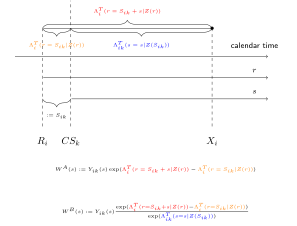
\includegraphics[width=0.95\linewidth]{figures/appendix//gong_schaubel_ipcw} 

}

\caption{Figure demonstrating how inverse probability censoring
weights (IPCW) are calculated for a subject $i$. Subject $i$ is
registered at $R_{i}$, is active at cross-section date $CS_{k}$, and
experiences an event at time $X_{i}$. Since subject $i$ has an active
registration at $CS_{k}$, this subject contributes an observation to the
data set. To correct for dependent censoring, the spell is weighted by
the inverse probability that patient $i$ is transplanted between
$CS_{k}$ and $X_{i}$, controlling for time-varying $Z( r )$
(type A weight). To this end, cumulative hazards treatment hazards are
estimated from registration $R_{i}$ to $CS_{k}$, and $R_{i}$ to $X_{i}$.
The type A weight is the inverse probability of being transplanted
before $X_{i}$, conditional on not being transplanted up to $CS_{k}$. It
is thus strictly greater than 1, thereby unstabilized. Gong and Schaubel
propose to normalize the type A weight by the conditional probability of
comparable subjects in cross-section $k$ experiencing an event between
$CS_{k}$ and $X_{i}$, conditional on the time-frozen covariate
information $Z( S_{ik} )$.}\label{fig:appfig1}
\end{figure}

Let \(R_{i}\) denote the registration date in calendar time for patient \(i\),
and \(r\) denote the time elapsed since patient \(i\)'s registration time \(R_{i}\).
Each patient has a waiting list death time (\(D_{i}\)), removal or censoring time
\(( C_{i} )\), and transplantation time \(T_{i},\) all defined
relative to the time origin \(R_{i}\). In general, only one of these events is
observable to us per patient, i.e., we observe \(X_{i} = \min( D_{i},C_{i},T_{i} )\).

Note that candidates for transplantation may become (temporarily) non-transplantable.
To account for this, let \(A_{i}( r )\) denote whether patient \(i\) has an active registration \(r\) time units after registration, i.e.,
\(A_{i}( r )\) = 1 only if patient \(i\) is eligible
for transplantation at calendar time \(R_{i} + r.\) In addition, updated
covariate information (for instance, MELD scores) may be reported for patient
\(i\). Denote with \(Z_{i}( r )\) all covariate history reported
up to \(r\) time units after registration for patient \({i}\). Note
that this covariate history can consist of observed covariates and other
summaries of treatment eligibility history (\(A_{i}( r )\)).

The key idea in Gong and Schaubel (2013) is to introduce a series
of cross-section dates (\(CS_{1},\ldots CS_{K})\), and model the mortality
hazard from each cross-section onwards for patients who have an active
registration at cross-section date \(CS_k\). These mortality hazard models are partly
conditional, which means they adjust only for covariate history observed prior to
\(CS_{k}\). The timescale the models use is the time elapsed since the cross-section
date \(CS_{k}\), which we denote by \(\text{s}\). For notational
convenience, it is helpful to define the time registered for patient \(i\)
until cross-section \(k\) by \(S_{ik}\), i.e.
\(S_{ik} = CS_{k} - R_{i}.\) Gong and Schaubel's approach can then be
represented with the following hazard model

\[
\lambda_{ik}^{D}( s ) = A_{i}( S_{ik} )\lambda_{0k}^{D}( s )\exp\left\{ \mathbf{\beta}_{\mathbf{0}}^{'}\mathbf{Z}_{\mathbf{i}}( S_{ik} ) \right\},\quad s > 0
\]

where \(A_{i}( S_{ik} )\) indicates patients are active
at the cross-section, \(\lambda_{0k}^{D}( s )\) is a baseline
hazard stratified by cross-section, and
\(Z_{i}( S_{ik} )\) is patient \(i\)'s covariate history
observed before cross-section date \(CS_{k}\).

Direct estimation of Equation A1 through Cox regression results in biased
\(\widehat{\beta_{0}}\), since covariate information (e.g., MELD) reported
after cross-section date \(CS_{K}\) may still affect the probability of
transplantation and waiting list mortality after \(CS_{k}\). To correct for
this, Gong and Schaubel propose weighing spells observed from cross
section \(CS_{k}\) to time \(r\) by the inverse conditional probability of
remaining on the waiting list up to time \(r\), i.e.

\[W_{\text{ik}}\left( r \right) = \left\lbrack P\left( T_{i} > r \middle| T_{i} > S_{\text{ik}},Z_{i}\left( t \right),t \leq r \right) \right\rbrack^{- 1} = \left\lbrack \frac{P\left( T_{i} > r \middle| Z_{i}\left( t \right),t \leq r \right)}{P\left( T_{i} > S_{\text{ik}} \middle| Z_{i}\left( t \right),t \leq S_{\text{ik}} \right)} \right\rbrack^{- 1}.\]

Gong and Schaubel refer to this weight as the ``type A'' weight. Note that
this weight is only defined as if the conditional probability of being
transplanted between the cross-section and \(r\) is strictly larger than
0. This assumption is known as positivity.

If we additionally assume that there is no unmeasured confounding of the
relation between transplantation and survival, IPCW can be used to
construct a ``pseudo-population'', which would have been observed if transplantation
had not existed. This means that under these assumptions, we can consistently
estimate \(\beta_0\) through Cox regression on the weighted population.

To construct this pseudo-population, we have to estimate these IPCW weights.
For this, Gong and Schaubel propose the following treatment hazard model:

\[\lambda_{i}^{T}\left( r \middle| Z_{i}\left( r \right) \right) = A_{i}\left( r \right)\lambda_{0}^{T}\left( r \right)\exp\left\{ \mathbf{\theta}_{\mathbf{0}}^{'}\mathbf{Z}_{\mathbf{i}}\left( r \right) \right\}.\]

This treatment hazard model use time since registration (\(r)\ \)as the
timescale, and adjusts for time-varying covariate information
(\(Z_{i}( r )\)). Using the definition of the hazard rate, one
can show that the type A weight reduces to

\[
\begin{aligned}
W_{ik}(r) 
  &= \left[ \frac{P\!\bigl(T_i > r \mid Z_i(t), t \le r\bigr)}
                 {P\!\bigl(T_i > S_{ik} \mid Z_i(t), t \le S_{ik}\bigr)} 
       \right]^{-1}\\
     &= \exp\!\Bigl[
            \int_{S_{ik}}^{r} A_i(u)\,\lambda_0^T(u)\,
                            \exp\{\theta_0' Z_i(u)\}\,du
       \Bigr],\\
  &= \exp\!\bigl[\Lambda_i^T(r) 
                \;-\;\Lambda_i^T\bigl(S_{ik}\bigr)\bigr].
\end{aligned}
\]

where
\(\Lambda_{i}^{T}\left( r \right) = \int_{0}^{r}{\lambda_{i}^{T}\left( u \middle| Z\left( u \right) \right)\text{du}}\)
is the cumulative hazard of transplantation.

The type A weight allows for unbiased estimation of \(\beta_{0}\) under no
unmeasured confounding and positivity. However, since
\(W_{ik}( r )\) is an inverse probability weight, it is
greater than or equal to 1 for all individuals and cross-sections. This
can result in instabilities when conditional probabilities become small.
To avoid this, Gong and Schaubel also propose to stabilize the type A
weight by a partial conditional estimate of the conditional probability
of being transplanted, i.e., stabilize \(W_{ik}( r )\)
with

\[P\left( T_{i} > r \middle| Z_{i}\left( S_{\text{ik}} \right),t \leq r \right).\]

Gong and Schaubel attain an estimate of this probability using the
following partly conditional treatment hazard model,

\[\lambda_{ik}^{T}( s ) = A_{ik}( s )\lambda_{0k}^{T}( s )\exp\left\{ \theta_{0}^{'}Z_{i}( S_{ik} ) \right\}.\]

Note that this model is partly conditional and uses time since
cross-section (\(s)\) as the timescale. Gong and Schaubel confirm with
simulations that empirically the type B weight results in smaller
standard errors than the type A weight. Also note that IPCW weights can be calculated both for the chance of obtaining a transplantation, as well as for the chance of being removed from the waiting
list. Under the assumption that waiting list removal and transplantation
are conditionally independent, a joint weight can be obtained which is the
product of IPCW weights for transplantation and IPCW weights for delisting.
Throughout part I of the thesis, we use these joint type B weights to correct
for dependent censoring by transplantation and delisting.

For the treatment and delisting hazard models, we adjust for a broad set of
confounders since IPCW relies on a no-unmeasured confounding assumption.
Patient factors adjusted for are sex, blood group, weight, listing country,
and age at listing. Clinical variables adjusted for are whether the patient
has a downgraded MELD, is simultaneously listed for a kidney, and the percentage
of time a patient has been non-transplantable (too good/too bad/other).
We directly adjust for MELD rather than MELD components, since Eurotransplant
allocates based on MELD. Since allocation is a national affair, we also
interact MELD with the patient country.

\chapter{Completing the status updates streams for transplant recipients}\label{APPimputation}

\chaptermark{Status update completion procedure}

The ELAS and ETKidney simulators require complete streams of status updates
to be available for all patient registrations, which means that every registration
must end with a waiting list removal (R) or death (D). However, most kidney or
liver candidates are transplanted, making these endpoints -- and any status
that would have occurred between transplantation and candidate death or removal --
unobserved. This is a general problem faced for the development of
discrete-event simulators for organ allocation. The SAM simulators address
it by matching transplant recipients to not-yet-transplanted patients based
on their predicted remaining lifetime, with remaining life time predicted using
a standard Cox model \citep{SRTR2019}. However, this
approach does address for repeated measures, does not match on other relevant
characteristics that might affect a candidate's health status trajectory (such as
disease group), and also does not correct for informative censoring from
transplantation, which can bias mortality estimates.

To address these limitations, we modify an existing statistical procedure from \citet{tayobstatistical2017} to complete the status update streams for patient
registrations in the ELAS and ETKidney simulators. This procedure constructs for every transplant recipient \(i\) a risk set of
\(R_i\) of not-yet-transplanted patients, who (a) have similar covariate profiles as patient \(i\) and (b)
have similar predicted remaining survival, where remaining survival is predicted
using methodology that accounts for repeated measures and corrects for informative
censoring. Algorithm B.1 summarizes this procedure. Steps 1 to 2 construct pseudo-observations for the expected log remaining survival time,
and Step 3 fits a model for log survival as a function of covariates.
These steps are performed once on the full cohort to estimate model
coefficients (\(\beta^{\text{PO}}\)). Step 4 is iteratively applied for each
transplant recipient, until their registration ends with a waiting list death (D)
or waiting list removal (R).

\begin{center}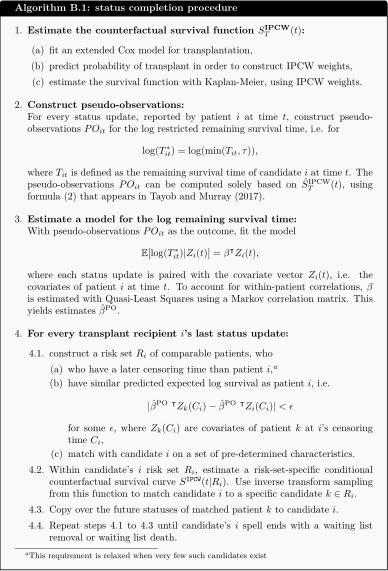
\includegraphics[width=1\linewidth]{figures/appendix/flowchart} \end{center}

\subsubsection*{Summary of Tayob and Murray (2017)}\label{summary-of-tayob-and-murray-2017}
\addcontentsline{toc}{subsubsection}{Summary of Tayob and Murray (2017)}

Algorithm B.1 uses statistical methodology developed by \citet{tayobstatistical2017}.
Tayob and Murray aim to model the 12-month restricted survival time \(T^* = \min(T, \tau)\)
of lung transplant candidates from pre-determined, regularly spaced landmark
times \(j = 1, ..., J\). To this end, they define
\(T^*_{ij}\) as the \(\tau\)-restricted remaining survival time of subject
\(i\) from landmark time \(j\), and use \(\tau = 12\) months in their application.
The central goal of their paper is to estimate
the expected log-survival time conditional on covariates, i.e.~to model
\[\mathbb{E}[\log(T^*) | Z] = \beta^\intercal Z.\]

They face three statistical challenges in the estimation of this model:

\begin{enumerate}
\def\labelenumi{\arabic{enumi}.}
\tightlist
\item
  \(T^*_{ij}\) is unobserved for most candidates due to censoring,
\item
  transplantation represents an informative censoring mechanism,
\item
  the \(T^*_{ij}\)s exhibit within-patient correlations across the landmark times \(j\).
\end{enumerate}

To address these challenges, Tayob and Murray proceed as follows:

\begin{enumerate}
\def\labelenumi{\arabic{enumi}.}
\item
  Tayob and Murray construct for each censored \(T^*_{ij}\) a risk set \(R_i\) of
  individuals who are (a) uncensored, (b) have similar expected survival
  as candidate \(i\), and (c) have similar covariates as patient \(i\). They construct
  these risk sets by following steps 1 through 4.1 of Algorithm B.1. In
  constructing these risk sets, Tayob and Murray require candidates to
  have similar covariate profiles to ensure that patients in the risk set are
  comparable despite the substantial heterogeneity of patients on the waiting
  list for lung transplantation. After step 4.1 of Algorithm B.1, Tayob and Murray derive
  \(M=10\) imputes of \(T^*_{ij}\) by inverse transform sampling from the risk-set
  specific survival function \(S^{\text{IPCW}}(t|R_i)\). They then use these
  imputes to fit the model
  \(\mathbb{E}[\log(T^*) | Z] = \beta^\intercal Z\), with
  coefficients pooled using Rubin's rules.
\item
  they use inverse probability censoring weighting (IPCW) to correct for informative
  censoring by transplantation in estimating the survival function in step 1 and step 4.2.
\item
  In estimating \(\mathbb{E}[\log(T^*)|Z] = \beta^\intercal Z\) in
  step 3 (and in their final step), Tayob and Murray address the
  within-patient correlations by fitting the model with
  Generalized Estimating Equations (GEE) with an unstructured
  working correlation matrix. This approach yields consistent
  estimates of \(\beta\) if the model is correctly specified (the
  correlation structure is allowed to be misspecified).
\end{enumerate}

Tayob and Murray conduct extensive statistical simulations to show that their
procedure can indeed estimate \(\mathbb{E}[\log(T^*) | Z] = \beta^\intercal Z\) with
minimal bias, and with similar efficiency to estimates obtained if censoring had never
occurred.

\newpage

\subsubsection*{Modifications to Tayob and Murray's procedure for Algorithm B.1.}\label{overview-of-the-counterfactual-future-status-imputation-procedure}
\addcontentsline{toc}{subsubsection}{Modifications to Tayob and Murray's procedure for Algorithm B.1.}

Tayob and Murray thus construct for every transplant recipient \(i\) a risk set
\(R_i\) of comparable patients, and use this risk set to sample imputes
for \(T^*_{ij}\). Our goal is to construct such a risk set \(R_i\), and use this
risk set to match candidate \(i\) to a
specific candidate \(k \in R_i\), who has similar remaining life time and covariates.
To achieve this, Algorithm B.1 has the following deviations from Tayob and Murray:

\begin{itemize}
\item
  Tayob and Murray only match censored candidates to non-censored candidates
  at specific landmark times \(j = 1, ..., J\). To enable discrete-event
  simulations, we must match transplant recipients to not-yet-transplanted
  candidates at the actual time of each transplant recipient's last known
  status update, which we denote by \(t\). The set of \(t\) is fully
  determined by the observed data, as the timings at which a
  candidate reports status update are not set by Eurotransplant.
  We define \(T^*_{it}\) as the restricted
  remaining survival time measured from \(t\) onwards, and construct
  pseudo-observations \(PO_{it}\) for the log restricted remaining survival time
  at time \(t\). This is done by steps 1 and 2 of Algorithm B.1.
\item
  The time points \(t\) correspond to any moment at which a candidate has
  reported a status update, and are therefore irregularly spaced and
  patient-specific. Because this makes the number of time points large, estimation of
  \(\beta^{\text{PO}}\) in step 3 using GEE with an unstructured working
  correlation matrix is infeasible. Instead, we estimate
  \(\beta^\text{PO}\) with Quasi-Least Squares (QLS) with a Markov correlation structure
  \citep{xieqls2010}. This structure assumes that the within-patient correlations
  between the pseudo-observations \(PO_{it}\) decay with their spacing in \(t\).
\item
  After step 4.2, Tayob and Murray use inverse-transform sampling from the
  risk-set-specific survival function \(S^{\text{IPCW}}(t|R_i)\) to sample imputes for
  \(T^*_{ij}\). We instead use inverse-transform sampling from \(S^{\text{IPCW}}(t|R_i)\)
  to match candidate \(i\) to a specific candidate \(k \in R_i\). We then copy over
  the status updates from patient \(k\) to patient \(i\), and
  repeat this step until all candidates have status updates that end with a
  waiting list removal (R) or (D) (see Step 4.4 of Algorithm B.1).
\end{itemize}

In the remainder of this appendix, we describe the steps of Algorithm B.1 in more detail.

For the ELAS simulator, Algorithm B.1 was run separately
for HU and elective candidates, with the time origin of \(t\) defined for both
candidate groups as the date a
candidate was listed for transplantation. For the HU model, we used \(\tau\)=14 days as the time horizon. For the elective candidates, we used \(\tau\)=90 days.

For the ETKidney simulator, Algorithm B.1 was run on all kidney
transplant candidates, with the time origin defined as the dialysis initiation date. A time horizon of 365 days was used (\(\tau=365\) days).

\newpage

\section{Step 1 and 2: Construction of the pseudo-observations}\label{step-1-and-2-construction-of-the-pseudo-observations}

\subsubsection*{Step 1: Consistent estimation of the survival function}\label{step-1-consistent-estimation-of-the-survival-function}
\addcontentsline{toc}{subsubsection}{Step 1: Consistent estimation of the survival function}

Algorithm B.1 requires us to consistently estimate the survival function in Step
1 and Step 4.2. A statistical challenge for this is that we have to deal with
informative censoring by transplantation. To correct for such informative
censoring, we use a Cox
model to predict the probability that a patient is transplanted over time,
and estimate the survival function weighing observations by their inverse probability of being transplanted.

For the ELAS simulator, this censoring model adjusted for recipient sex,
recipient blood group, spline terms of recipient weight and age, recipient
disease group, percentage of time NT (total/too bad/too good), the national
match MELD, whether the patient is on dialysis, whether the patient has a downmarked
MELD score, and whether the patient has an exception (Y/N).

For the ETKidney simulator, this censoring model adjusted for are candidate sex,
candidate blood group, spline terms of candidate age, the disease group (congenital,
polycystic, neoplasms, diabetes, glomerular disease, renovascular / vascular disease,
tubular and interstitial disease, or other), the HLA-ABDR mismatch frequency
(defined in Section \ref{sec:etkidneymmp})

Figure \ref{fig:chappsfig2} shows estimated survival functions
without (orange) and with (blue) correction for dependent censoring for
elective liver transplantation patients, stratified by their laboratory MELD score at listing. The estimates of the 90-day survival probabilities decrease
due to
inverse probability weighting, with 90-day waiting list survival
estimated with IPCW up to 7.4\% lower for MELD 25--29 than 90-day waiting
list survival estimated without IPCW. This is expected, as candidates who
are deteriorate on the waiting list have a higher probability of being
transplanted on the waiting list.

With these censoring models, we can construct IPCW weights for each patient, based on the predicted probability
of being transplanted at each time point. Using these IPCW weights, we then
estimate the counterfactual survival function with the Kaplan--Meier estimator.
This approach allows us to consistently estimate the survival function under
dependent censoring, as required for step 1 of Algorithm B.1.

\begin{figure}[ht]

{\centering 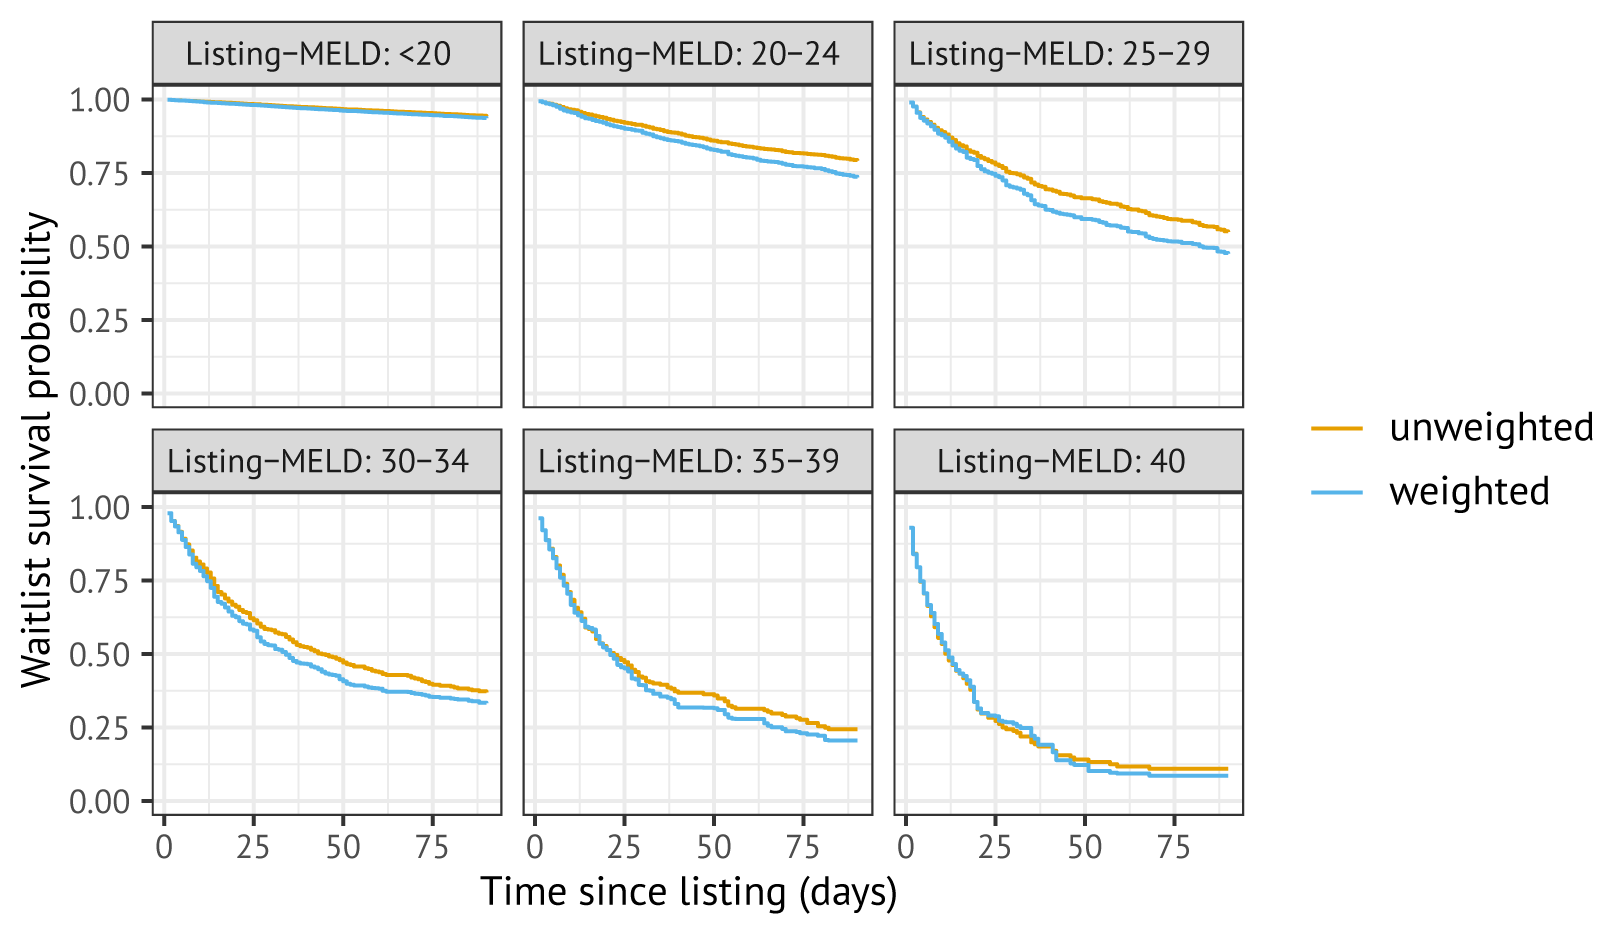
\includegraphics[width=0.9\linewidth]{figures/appendix//sfig2-estimated_event_probs} 

}

\caption{Estimated survival probabilities estimated in the cohort, with (blue) and without (orange) Inverse Probability Censoring Weighting to correct for informative censoring by transplantation.}\label{fig:chappsfig2}
\end{figure}

\newpage

\subsubsection*{Step 2: Construction of pseudo-observations}\label{step-2-construction-of-pseudo-observations}
\addcontentsline{toc}{subsubsection}{Step 2: Construction of pseudo-observations}

To predict the expected remaining lifetime for candidates on the waiting list,
we directly model candidate's expected residual remaining survival time \(T^{*}\) using:
\[\mathbb{E}[\log(T^*)|Z] = \beta^\intercal Z.\] For this, we
would ideally know the remaining time-to-event \(T^*_{it}\) for
all patients \(i\) and status update times \(t\). However, censoring and
transplantation within \(\tau\) time units of \(t\) prevent us from
observing \(T^*_{it}\). Formula (2) of \citet{tayobstatistical2017} describes
how pseudo-observations for \(\log(T_{ij}*)\) can be constructed using
only the survival function \(\hat{S}^{\text{IPCW}}(t)\)
that was estimated in Step 1 of Algorithm B.1.
We used this formula to calculate pseudo-observations \(PO_{it}\) for
\(\log(T^*_{it})\). Armed with pairs \((PO_{it}, Z_i)\), we can
estimate \(\beta^{PO}\) in step 3 of Algorithm B.1.
\newpage

\section{Step 3: Fitting a model for the mean restricted survival time}\label{step-3-fitting-a-model-for-the-mean-restricted-survival-time}

With pairs \((PO_{it}, Z_i)\) we can model the expected log remaining
survival time as

\[
\mathbb{E}[\log(T^*) \mid Z] = \beta^\intercal Z
\tag{B.1}
\]

A statistical challenge to estimating \(\beta\) is that we have
to deal with the within-patient correlations in \(PO_{it}\) across
status update times \(t\). Tayob and Murray
faced a similar issue, with correlations between \(T^*_{ij}\)
over the landmark times \(j\). They addressed this issue by estimating
\(\beta\) with Generalized Estimating Equations (GEE) with an unstructured
correlation matrix correlation over the landmark times \(j\) (which
requires \(j(j+1)/2\) parameters). This allows for consistent estimation of
\(\beta\), even if the correlation structure is misspecified.

Unfortunately, this specific estimation strategy is not feasible in our setting: in our case, the pseudo-observations \(PO_{it}\)
are indexed by \(t\), i.e., all the timings at which candidates reported status
updates to Eurotransplant, which would blow up the dimensions
for an unstructured working correlation matrix. To
estimate the model, we instead estimate
the model with Quasi-Least Squares with a Markov correlation structure \citep{Shults2014-di}. This Markov correlation
structure assumes that the correlation between measurements
\(PO_{is}\) and \(PO_{it}\) decays with their separation in time:
\[\texttt{Corr}(PO_{is}, PO_{it}) = \alpha^{|s-t|}.\] Parameters
\(\alpha\) and \(\beta\) of this model can be estimated with the \texttt{qlspack} R
package \citep{xieqls2010}. With this approach, \(\beta\) can also
be consistently estimated even if the correlation structure is
misspecified.

For the ELAS simulator, we use different model specifications for HU
and elective patients for equation B1. For HU patients, the covariates
include recipient age at registration, the laboratory MELD score, whether the
patient is on biweekly dialysis, recipient sex, and disease group. For
elective patients, we adjust for age at registration, recipient weight,
MELD components (serum creatinine, bilirubin, INR, biweekly dialysis),
recipient sex, disease group, cirrhosis etiology, type of exception
score, whether it is a repeat transplant candidate, and whether the patient
has failed to re-certify their MELD score. Continuous variables are
transformed with spline terms.

For the ETKidney simulator, we use covariates for candidate age, candidate sex,
whether the candidate has previously received a kidney transplantation,
as well as the time the candidate has waited on the kidney waiting list.

\newpage

\section{Step 4: Constructing future statuses}\label{step-4-constructing-future-statuses}

To complete the set of status updates for transplant recipient \(i\),
we first construct a risk set \(R_i\) of not-yet-transplanted candidates who
are comparable to the transplant recipient (step 4.1).
As in Tayob and Murray, a minimum requirement to match transplanted
candidates to not-yet-transplanted candidates is:
\[|\hat{\beta}^{\text{PO}}\ ^\intercal Z_k(C_{i}) - \hat{\beta}^{\text{PO}}\ ^\intercal Z_i(C_{i})| < 0.50,\]
i.e., candidates have similar expected log restricted survival.

We additionally require candidates to match on other covariates,
as is done by Tayob and Murray. A motivation for requiring candidates to
also match on covariate profiles is that organ waiting lists are highly
heterogeneous, and we want to ascertain that the candidate's risk set
only consists of patients that are actually comparable to the patient. For example, by matching on disease groups for
liver transplantation candidates, we can prevent that a candidate
with chronic liver cirrhosis is matched to a candidate with hepatocellular
carcinoma, even if these patients have similar predicted remaining
survival time.

For the ELAS simulator, we require candidates to always match on pediatric status. For other discrete and continuous variables, we use an adaptive matching procedure,
in which we strive towards \(|R_i|\) = 35 candidates in the risk set for HU patients, and \(|R_i|\) = 50
candidates for non-HU patients. Specifically, the discrete variables used for matching are

\begin{enumerate}
\def\labelenumi{\arabic{enumi}.}
\tightlist
\item
  whether the patient is a repeat transplant candidate
\item
  current urgency code (non-transplantable)
\item
  (N)SE group
\item
  disease group
\item
  urgency reason (NT too good / NT other / NT too bad)
\item
  biweekly dialysis (twice in week preceding MELD measurement)
\item
  recipient country.
\end{enumerate}

Continuous match variables used are the laboratory MELD score, age at
registration, (N)SE MELD score (for elective patients only), where we
restrict absolute differences in continuous variables to pre-determined
caliper widths (lab-MELD: 5, age: 15 years, (N)SE-MELD: 5). In case
matching according to all criteria fails to result in a risk set of
sufficient size, we drop a discrete match criterion (from 7 to 1 in the
list above). In case dropping all discrete match criteria does not
result in adequately sized risk set, we increase caliper widths for
continuous variables. In total, about 50\% of transplant recipients can
be matched to a risk set on all characteristics, and 80\% of
transplant recipients can be matched on
the first 4 discrete variables (with the most restrictive caliper
widths).

For the ETKidney simulator, we always match candidates on whether they have
had a previous kidney transplantation, as well as whether they have an active
waiting list status. The procedure also tried to match candidates based on disease group, reason why they were non-transplantable, and candidate country of listing. These constraints were relaxed in case fewer than 50 candidates could be
included in the risk set. Finally, the procedure also imposed constraints on the
differences in accrued dialysis time and age at listing using pre-determined
caliper widths.

\subsubsection*{Example of a constructed risk set for the ELAS simulator}\label{example-of-a-constructed-risk-set-for-the-elas-simulator}
\addcontentsline{toc}{subsubsection}{Example of a constructed risk set for the ELAS simulator}

In Table \ref{tab:appBtab1} we show an example of a constructed
risk set for a patient who was transplanted, and for whom we had to
complete their status update trajectory. The first row of Table
\ref{tab:appBtab1} shows that this transplant recipient was listed in 2014
in Germany at an age of 64 for cirrhosis. The
patient reported a lab-MELD score equal to 33 points 36 days after
registration, and was
transplanted 6 days later. Based on our model (equation B1), the
expected log residual survival time for this patient is approximately 3.51,
which corresponds roughly to 34 days of remaining lifetime.

The other rows of Table \ref{tab:appBtab1} show 10 of the candidates
who were present in patient \(i\)'s risk set \(R_i\). These patients remain at
risk 36 days after waiting list registration (\(\min(C_{k}, T_k) > C_i\))
and are similar in terms of predicted expected log survival. Turning to
other characteristics, we see that the matching procedure did not match
on listing country and receival of biweekly dialysis. The risk set is
comparable in terms of continuous variables (lab-MELDs ranging from 28
to 38, ages from 53 to 69).

\begin{table}[!h]
\centering
\caption{\label{tab:appBtab1}Example of the risk set $R_i$ for a selected liver transplant recipient.}
\centering
\resizebox{\ifdim\width>\linewidth\linewidth\else\width\fi}{!}{
\fontsize{10}{12}\selectfont
\begin{tabular}[t]{llllllllllllll}
\toprule
year & status time $t$ & $C_k$ & $T_k$ & $\exp(\hat{\log(T^*)})$ & lab-MELD & age & ped. & reTX & urg & (N)SE & diag. & dial. & country\\
\midrule
\addlinespace[0.3em]
\multicolumn{14}{l}{\textbf{transplant recipient}}\\
\hspace{1em}2014 & 36.0 & 41.9 & - & 33.7 & 33 & 64 & 0 & 0 & T & none & Cirrh. & 1 & DE\\
\addlinespace[0.3em]
\multicolumn{14}{l}{\textbf{risk set}}\\
\hspace{1em}2012 & 40.1 & 46 & - & 32.8 & 34 & 65 & 0 & 0 & T & none & Cirrh. & 0 & DE\\
\hspace{1em}2015 & 41.1 & 55.8 & - & 34.9 & 30 & 63 & 0 & 0 & T & none & Cirrh. & 1 & DE\\
\hspace{1em}2013 & 40.1 & 47.9 & - & 32.4 & 38 & 56 & 0 & 0 & T & none & Cirrh. & 1 & DE\\
\hspace{1em}2012 & 36.4 & 42.1 & - & 35.3 & 35 & 68 & 0 & 0 & T & none & Cirrh. & 1 & BE\\
\hspace{1em}2010 & 40.2 & 58.9 & - & 35.5 & 28 & 68 & 0 & 0 & T & none & Cirrh. & 0 & DE\\
\hspace{1em}2016 & 37.7 & 86.3 & - & 35.6 & 34 & 53 & 0 & 0 & T & none & Cirrh. & 1 & DE\\
\hspace{1em}2009 & 41.8 & - & 84.8 & 36.3 & 33 & 53 & 0 & 0 & T & none & Cirrh. & 0 & DE\\
\hspace{1em}2008 & 35.1 & 42.1 & - & 29.9 & 30 & 69 & 0 & 0 & T & none & Cirrh. & 0 & DE\\
\hspace{1em}2012 & 37.3 & 44.9 & - & 38.4 & 37 & 64 & 0 & 0 & T & none & Cirrh. & 0 & BE\\
\hspace{1em}2010 & 7.4 & - & 946.9 & 29.4 & 29 & 63 & 0 & 0 & T & none & Cirrh. & 0 & AU\\
\bottomrule
\end{tabular}}
\end{table}

\FloatBarrier

Within risk set \(R_i\), we can obtain a
personalized estimate of the conditional probability of the candidate \(i\)'s
survival \(t\) time units after their censoring time (i.e.
\(\hat{S}^{\text{IPCW}}_T(t|R_i, T > C_i)\)). For the 64-year-old, German
transplant candidate discussed in Table \ref{tab:appBtab1}, the survival function estimated using Kaplan-Meier with IPCW in their risk set \(R_i\) is shown by Figure \ref{fig:chappsfig3}. This suggests that the 64-year old candidate with a MELD score of 33 would
have a waiting list death probability of approximately 60\% in the 90 days following their censoring time.

\begin{figure}[ht]

{\centering 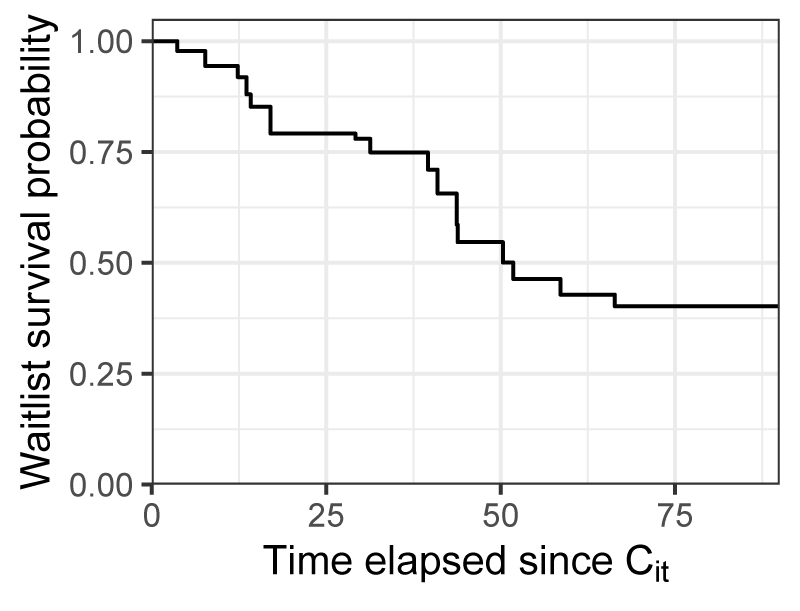
\includegraphics[width=0.5\linewidth]{figures/appendix//sfig3-survival_selected_riskset} 

}

\caption{Conditional survival function, estimated with inverse probability censoring weighting for the risk set $R_i$, where $i$ is the 64-year-old German candidate appearing in Table B.1.}\label{fig:chappsfig3}
\end{figure}

\subsubsection*{Example of a constructed risk set for the ETKidney simulator}\label{example-of-a-constructed-risk-set-for-the-etkidney-simulator}
\addcontentsline{toc}{subsubsection}{Example of a constructed risk set for the ETKidney simulator}

Table \ref{tab:appBtab2} shows an example of a constructed
risk set for a female candidate who was transplanted after waiting for
4.5 years for a kidney transplantation with 6 years of accrued dialysis
time in total. The first row of Table \ref{tab:appBtab2} shows that this
transplant recipient was listed in 2014 in Germany for polycystic kidney disease. The remaining
rows of Table \ref{tab:appBtab2} show 10 (out of 50) waiting list
candidates in patient \(i\)'s risk set \(R_i\). These patients remain at
risk having waited 2162 days on dialysis for transplantation. They are
also similar to the patient in terms of other covariates: all matched
candidates are patients with polycystic kidney disease waiting in
Germany, and around age 60.

\begin{table}
\centering
\caption{\label{tab:appBtab2}Example of the risk set $R_i$ for a selected kidney transplant recipient. Note that matching in the ETKidney simulator
  is based on dialysis vintage, not waiting time.}
\centering
\resizebox{\ifdim\width>\linewidth\linewidth\else\width\fi}{!}{
\fontsize{10}{12}\selectfont
\begin{tabular}[t]{llllllllll}
\toprule
year & waiting time & $C_i$ & $T_i$ & dialysis vintage & age & repeat transplant & urg. & diag & country\\
\midrule
\addlinespace[0.3em]
\multicolumn{10}{l}{\textbf{Transplant recipient}}\\
\hspace{1em}2014 & 1602 & 1618 & - & 2162 & 64 & 0 & T & Polycystic & DE\\
\addlinespace[0.3em]
\multicolumn{10}{l}{\textbf{Risk set}}\\
\hspace{1em}2017 & 1506 & 2229 & - & 1965 & 62 & 0 & T & Polycystic & DE\\
\hspace{1em}2010 & 1595 & - & 2346 & 2410 & 62 & 0 & T & Polycystic & DE\\
\hspace{1em}2012 & 1635 & - & 2837 & 2495 & 61 & 0 & T & Polycystic & DE\\
\hspace{1em}2014 & 1961 & - & 2619 & 1905 & 62 & 0 & T & Polycystic & DE\\
\hspace{1em}2016 & 1467 & - & 1747 & 2009 & 59 & 0 & T & Polycystic & DE\\
\hspace{1em}2015 & 1775 & 2255 & - & 2245 & 59 & 0 & T & Polycystic & DE\\
\hspace{1em}2016 & 1464 & - & - & 1869 & 58 & 0 & T & Polycystic & DE\\
\hspace{1em}2019 & 1567 & - & - & 2499 & 58 & 0 & T & Polycystic & DE\\
\hspace{1em}2010 & 1459 & 2333 & - & 1991 & 58 & 0 & T & Polycystic & DE\\
\hspace{1em}2011 & 1686 & 3531 & - & 1898 & 61 & 0 & T & Polycystic & DE\\
\bottomrule
\end{tabular}}
\end{table}

\FloatBarrier

\section{Step 4.2: Matching the patient to a particular patient in the risk set}\label{step-4.2-matching-the-patient-to-a-particular-patient-in-the-risk-set}

The aim of step 4.2 in Algorithm B.1 is to match censored patient \(i\) to a single candidate \(k\) from their risk set (\(k\in
R_i\)). We do this by inverse transform sampling from the
risk-set-specific survival function
\(\hat{S}^{\text{IPCW}}_T(t\,|\,R_i,\, T > C_i)\). Specifically, we
(i) draw a random number \(u\) from the uniform distribution, and
(ii) find the smallest time \(t\) such that \(\hat{S}^{\text{IPCW}}_T(t\,|\,R_i,\, T > C_i) \leq u\).

If such a \(t\) exists, it corresponds to the observed event
(removal or death) time of some patient \(k \in R_i\). We therefore
complete the status update trajectory for patient \(i\) by copying
over the future status updates of this patient \(k\).

If no such \(t\) exists within the truncation time horizon \(\tau\),
this means patient \(i\) would be alive and remain waitlisted
\(\tau\) days after their censoring time. In this case, we select a
candidate from those with censored restricted survival times,
i.e., from the set \(\{k \in R_i : T_k > C_i + \tau\}\). Among
these, a single patient is randomly chosen with sampling
probabilities proportional to their IPCW weights at time \(\tau\).

We note that this procedure can also match a transplant recipient to
another patient who receives a transplant. In that case, we still
copy over all subsequent status updates from the matched candidate,
excluding the transplant event itself. In those cases, Step 4
of Algorithm B.1 is iteratively applied, until the candidate's
registration ends with a removal (R) or death (D) status.

\chapter*{Summary}\label{summary}
\addcontentsline{toc}{chapter}{Summary}

\addcontentsline{toc}{chapter}{Summary}
\markboth{SUMMARY}{SUMMARY}

Every year, more than 6,000 organ transplantations are performed in the eight
European countries that participate in Eurotransplant. Despite this, the persistent
shortage of donor organs means that about 1,000 patients die annually while waiting for
an organ transplantation.

Eurotransplant is responsible for offering the deceased-donor organs to
the candidates who await a transplantation. To which patient Eurotransplant makes
an offer is determined by allocation rules, which have been shaped by almost six decades of
scientific, legal, and ethical discussions between Eurotransplant and
the national competent authorities of the eight member countries. Eurotransplant
has implemented these rules in allocation algorithms, which determine which candidates
are eligible to receive an organ offer, and in what order they ought to be contacted.

A central goal of Eurotransplant's allocation systems is that patients should have an equal opportunity
of receiving a transplant. A first goal of this thesis is to study research questions
relating to such equality of opportunity. Our results show there is room
for improvement. For example, female patients on the liver waiting list are more
likely to experience an adverse outcome than male patients. We link
this disparity to the smaller body size of female transplantation candidates --
and not sex itself, as is suggested by the existing literature. Similarly,
kidney transplant candidates who are immunized face reduced access to transplantation
under the current rules. This latter disadvantage persist even though Eurotransplant
has implemented special mechanisms to support these groups.

One reason why such disadvantages persist is that Eurotransplant lacks the tools
to quantify the impact of policy changes. This complicates discussions within
Eurotransplant's advisory committees on how the allocation can be improved. To
overcome this barrier, the second goal of this thesis is to develop discrete-event
simulators for liver and kidney allocation. These tools allow Eurotransplant
to assess the impact of alternative allocation policies on waiting list outcomes,
and can facilitate collaborations with clinicians, policymakers, and other stakeholders on how
allocation can be improved. We validated these simulation
tools on historic data, and the simulators already support discussions within
Eurotransplant on how policies can be improved. For example, the liver simulator
has been used to support discussions on switching to a new score for liver allocation.

Although these tools do not eliminate the difficult ethical trade-offs involved
in organ allocation, they help Eurotransplant by making these trade-offs explicit.
Thereby, the simulators can pave the way for a more informed and constructive dialogue
among clinicians, policymakers, and other stakeholders on how the allocation of
deceased-donor organs can be improved.

\chapter*{Course of Life}\label{course-of-life}
\addcontentsline{toc}{chapter}{Course of Life}

\addcontentsline{toc}{chapter}{Course of Life}
\markboth{COURSE OF LIFE}{COURSE OF LIFE}

Hans de Ferrante was born on March 20, 1995 in 's-Gravenhage, the Netherlands. He completed his secondary education at St.~Odulphus-Lyceum in Tilburg.

In 2013, Hans began his academic journey at Eindhoven University of Technology, where he pursued a Bachelor of Science in Biomedical Engineering. For this degree, he focused on molecular biology, organic chemistry, and computational biology. In 2014, Hans started a second Bachelor of Science in Econometrics and Operations Research at Tilburg University. He graduated cum laude for these degrees in 2017 and 2018, respectively. During his undergraduate studies, Hans took part in the iGEM competition in Boston, spent a semester abroad at the University of Hong Kong, and participated in the Netherlands-Asia Honours Summer School (NAHSS) in Chengdu, China.

Hans continued his studies with a Master of Science in Systems Biology and Bioinformatics at the Vrije Universiteit and Universiteit van Amsterdam. For this degree, he wrote a master's thesis on protein-protein interface prediction from amino acid sequence, and he served as a teaching assistant for several bioinformatics courses. Parallel to this, Hans pursued a Master of Science in Econometrics and Mathematical Economics at Tilburg University. Hans wrote his master's thesis for Econometrics and Mathematical Economics while working as a data science intern at Pacmed in Amsterdam. The topic of this thesis was causal inference for the treatment of breast cancer, using national registry data maintained by Integraal Kankercentrum Nederland (IKNL). He graduated cum laude for both degrees in 2020. From 2018 to 2020, Hans also worked as a part-time research assistant in data science at CentERdata in Tilburg.

Hans started his PhD project at Eindhoven University of Technology under the
supervision of dr. Bart Smeulders and prof.dr. Frits Spieksma in September 2020.
His research focuses on liver and kidney allocation in Eurotransplant. This
thesis presents results of this research.

Hans will defend his thesis at Eindhoven University of Technology on July 3rd, 2025.

\chapter*{List of publications}\label{list-of-publications}
\addcontentsline{toc}{chapter}{List of publications}

\addcontentsline{toc}{chapter}{Publications}
\markboth{PUBLICATIONS}{PUBLICATIONS}

\subsubsection*{Journal articles}\label{journal-articles}
\addcontentsline{toc}{subsubsection}{Journal articles}

\begin{itemize}
\item
  Hans de Ferrante, Marieke de Rosner-van Rosmalen, Bart M.L. Smeulders, Frits C.R. Spieksma, and Serge Vogelaar (2025). \emph{A discrete event simulator for policy evaluation in deceased-donor liver allocation in Eurotransplant}. In: \emph{Operations Research, Data Analytics and Logistics}.
\item
  Hans de Ferrante, Marieke de Rosner-van Rosmalen, Bart M.L. Smeulders, Serge Vogelaar, and Frits C.R. Spieksma (2025).\\
  Sex disparity in liver allocation within Eurotransplant. In: \emph{American Journal of Transplantation}.
\item
  Hans de Ferrante, Bart Smeulders, Ineke Tieken, Sebastiaan Heidt, Geert W. Haasnoot, Frans H.J. Claas, Serge Vogelaar, and Frits Spieksma (2023). \emph{Immunized Patients Face Reduced Access to Transplantation in the Eurotransplant Kidney Allocation System}. In:
  \emph{Transplantation}.
\item
  Hans de Ferrante, Marieke de Rosner-van Rosmalen, Bart M.L. Smeulders, Serge Vogelaar, Frits C.R. Spieksma (2024). \emph{Revising model for end-stage liver disease from calendar-time cross-sections with correction for selection bias}. In: \emph{BMC Medical Research Methodology}.
\end{itemize}

\subsubsection*{Pre-prints}\label{pre-prints}
\addcontentsline{toc}{subsubsection}{Pre-prints}

\begin{itemize}
\tightlist
\item
  Hans de Ferrante, Rocio Laguna Goya, Bart M.L. Smeulders, Frits C.R. Spieksma, and Ineke Tieken (2025). \emph{The ETKidney simulator: a discrete event simulator to assess the impact of alternative kidney allocation rules in Eurotransplant}. \emph{arXiv:2502.15001}.
\end{itemize}

\backmatter
{
\small
\bibliography{thesis.bib}
}

\end{document}
